\PassOptionsToPackage{unicode}{hyperref}
\documentclass[a4paper,twoside]{memoir}
\usepackage{silence}
\setcounter{tocdepth}{8}
\setcounter{secnumdepth}{-1}
\WarningFilter{hyperref}{Token not allowed in a PDF}
\WarningFilter{hyperref}{Difference (2)}
\directlua{}
\usepackage{xcolor}
\definecolor{myred}{rgb}{0.7, 0.11, 0.11}

\definecolor{bleu}{rgb}{0.19, 0.55, 0.91}
\definecolor{mygold}{rgb}{0.85, 0.65, 0.13}
\definecolor{darkgrey}{rgb}{0.52, 0.52, 0.51}
\setcounter{secnumdepth}{0}
\newcommand{\guidancesection}[1]{\section*{\color{darkgrey}#1}    \addcontentsline{toc}{section}{\color{darkgrey}#1}}
\newcommand{\ocsection}[1]{\section*{\color{bleu}#1}    \addcontentsline{toc}{section}{\color{bleu}#1}}
\newcommand{\ocsubsection}[1]{\subsection*{\color{bleu}#1}    \addcontentsline{toc}{subsection}{\color{bleu}#1}}

\newcommand{\cdsubsection}[1]{\subsection*{\color{mygold}#1}    \addcontentsline{toc}{subsection}{\color{mygold}#1}}
\newcommand{\rulesection}[1]{\section*{\color{myred}#1}    \addcontentsline{toc}{section}{\color{myred}#1}}
\newcommand{\mysec}[1]{\section*{#1}    \addcontentsline{toc}{section}{#1}}
\newcommand{\guidancesubsection}[1]{\subsection*{\color{darkgrey}#1}    \addcontentsline{toc}{subsection}{\color{darkgrey}#1}}
\newcommand{\rulesubsubsection}[1]{\subsubsection*{\color{myred}#1}    \addcontentsline{toc}{subsubsection}{\color{myred}#1}}

\newcommand{\rulesubsection}[1]{\subsection*{\color{myred}#1}    \addcontentsline{toc}{subsection}{\color{myred}#1}}
\newcommand{\guidancesubsubsection}[1]{\subsubsection*{\color{darkgrey}#1}    \addcontentsline{toc}{subsubsection}{\color{darkgrey}#1}}
\colorlet{MYGOLD}{mygold}
\colorlet{DARKGREY}{darkgrey}
\colorlet{MYRED}{myred}
\colorlet{BLEU}{bleu}
\usepackage{fontspec}
\setmainfont[Ligatures=TeX,
Scale=.96, 
RawFeature={+pnum,+lnum},
SmallCapsFeatures={LetterSpace=15,RawFeature={+smcp},},
BoldFeatures = {
RawFeature={+pnum,+lnum,+liga},
SmallCapsFont= {PalatineParliamentary-Bold},SmallCapsFeatures={%
RawFeature={+smcp,+pnum,+lnum,+liga}%
},},
Numbers={OldStyle},
	Ligatures={TeX,Common},
BoldFont={PalatineParliamentary-Bold}, 
 ItalicFont={PalatineParliamentary-Italic},
  ItalicFeatures={
  RawFeature={+liga,+pnum,+lnum},
},
 BoldItalicFont={PalatineParliamentary-BoldItalic}
]{PalatineParliamentary-Regular}



\directlua{}
\title{Code of Conduct}
\author{Bar Standards Board}
\newcommand\chap[1]{
    \chapter*{#1}
    \addcontentsline{toc}{chapter}{#1}
    \markboth{#1}{#1}}
\usepackage[margin=2in,headheight=24pt]{geometry}
\newcommand{\hide}[1]{}
\usepackage[hidelinks]{hyperref}
\usepackage{enumitem}
\newlist{numlist}{enumerate}{3}
\setlist[numlist]{label=(\arabic*)}
\newlist{romlist}{enumerate}{3}
\setlist[romlist]{label=(\roman*)}
\newlist{alphlist}{enumerate}{3}
\setlist[alphlist]{label=(\emph{\alph*})}
\newlist{Alphlist}{enumerate}{3}
\setlist[Alphlist]{label=(\emph{\Alph*})}
\newlist{dotlist}{enumerate}{3}
\setlist[dotlist]{label=•}
\newlist{dashlist}{enumerate}{3}
\setlist[dashlist]{label=--}
\newcommand{\nl}{\begin{numlist}}
\renewcommand{\ln}{\end{numlist}}	
\newcommand{\al}{\begin{alphlist}}
\newcommand{\all}{\begin{alphlist}}
\newcommand{\la}{\end{alphlist}}	
\newcommand{\rl}{\begin{romlist}}
\newcommand{\lr}{\end{romlist}}	

\setlength{\parindent}{1.25em}
\usepackage{graphicx}
\usepackage{pdfpages}
\begin{document}
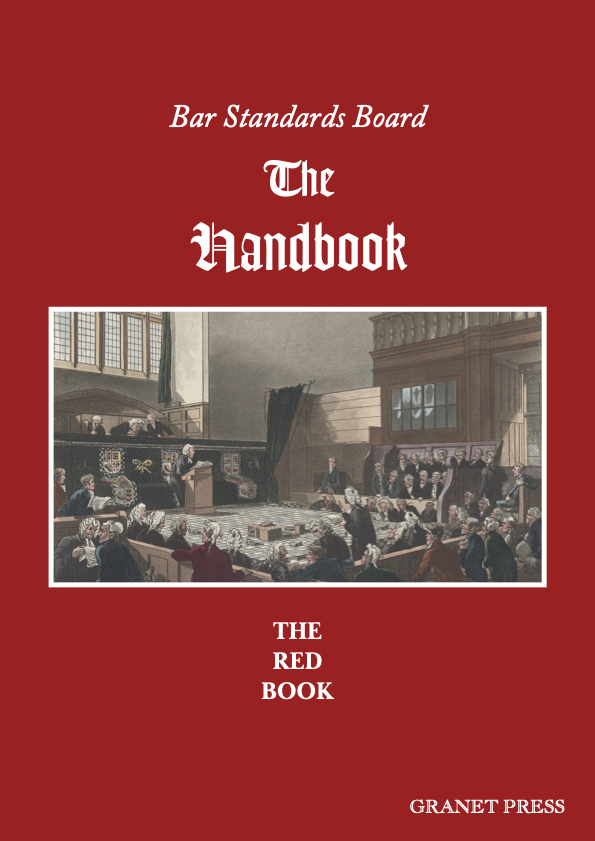
\includepdf{cover-page.pdf}
\cleartoverso
\frontmatter
\begin{KeepFromToc}
  \tableofcontents
\end{KeepFromToc}
\chapter{BSB Chair’s introduction to Handbook}

The BSB Handbook has set the standards of conduct for barristers since 2014. It serves as the key regulatory tool through which we can ensure the effective administration of justice is served. Barristers are central to the justice system, and clients depend upon their independence and ability to present their case fearlessly and effectively whilst providing a high standard of service.

We want the Handbook to be accessible for barristers, users of barristers’ services, and the general public. Our aim is that the Handbook should allow consumers to understand what to expect from barristers as well as providing clarity about the regulatory regime with which barristers must comply. But we recognise that, as it has developed over the years, the Handbook has become less easy to use and we have therefore announced a review of the Handbook to ensure that it remains fit for purpose, relevant, and accessible.

The Handbook also ensures that clients of barristers’ services receive the same level of protection and service regardless of the vehicle through which that service is provided. We now regulate a range of entities, including some alternative business structures. The Handbook ensures the public can be confident that the same standards apply to these different business structures as well as individual barristers.

\medskip
\hfill\scshape Baroness Tessa Blackstone

\normalfont\hfill\itshape Chair of the BSB
\normalfont
\chapter{Handbook Release Notes}
\section*{Version 4.6 (31 December 2020) - changes}
Version 4.6 of the BSB Handbook came into force at the end of the transition period following the UK’s exit from the EU. The changes affect Registered European Lawyers (RELs) practising at the Bar of England and Wales, and European lawyers seeking to be admitted to the Bar. They also implement provisions relating to the Swiss Citizens’ Rights Agreement, which was agreed by the UK and Switzerland in 2018. You can read more about the BSB’s regulation and the UK’s exit from the EU on our website here.

\section*{Version 4.5 (September 2020) - changes}
The new Internal Governance Rules, set by the Legal Services Board (LSB), aim to further enhance the BSB’s regulatory independence and Version 4.5 of the Handbook therefore reflects the requirements of the new rules.

Version 4.5 also includes amendments to the Disciplinary Tribunal Rules which enable Disciplinary Tribunals to rely on wasted cost orders as proof of conduct occurring, and clarify that Directions Judges have the discretion to make cost orders.

In addition, version 4.5 includes updated guidance on Core Duty 9, making clear that barristers’ duty to co-operate with their regulators includes all relevant regulators and ombudsman schemes.

\section*{Version 4.4 (February 2020) - Changes}
A new rule (Rule C85A) has been introduced in Version 4.4 to prevent barristers from supervising immigration advisers who have been subject to serious sanctions by the Office of the Immigration Services Commissioner (OISC) or a legal regulator. Barristers must also have regard to the updated guidance on supervising immigration advisers.

\section*{Version 4.3 (October 2019) - Changes}
Version 4.3 of the Handbook includes the new Enforcement Decision Regulations, contained in Part 5:A, which replace the old Complaints Regulations. The new Regulations were designed to improve the way that the BSB assesses and handles reports about persons we regulate.

The Regulations remove the distinction between “complaints” and other types of information received, to allow for a more holistic approach to addressing concerns about those whom we regulate. Information that requires assessment is referred to as a “report”, regardless of its source. A report can be treated as an allegation and formally investigated if it reveals a potential breach of the BSB Handbook.

Two new roles have been created to take regulatory decisions – the Commissioner and the Independent Decision-Making Body – following the disestablishment of the Professional Conduct Committee. The powers and functions of each role are set out in the Regulations, including the decisions available to each role at the end of the investigation of an allegation. The Commissioner’s powers include the power to authorise other persons to exercise any powers, and these authorisations are recorded in the Scheme of Delegations, contained in the Bar Standards Board Governance Manual.

\section*{Version 4.2 (September 2019) - Changes}
\subsection*{Scope of Practice - Employed Barristers in Non-Authorised Bodies}

rS39 sets out who employed barristers in non-authorised bodies are permitted to supply legal services to. They are normally only permitted to supply services to their employer i.e. the body itself, and not clients of their employer.

New guidance (gS8A - gS8C) clarifies that the following arrangements are permissible, and barristers seeking to work in these ways do not need to obtain waivers from rS39:
\begin{dotlist}
\item Barristers providing services through a non-authorised body (e.g. an agency or corporate vehicle) whose purpose is to facilitate the supply of in-house legal services to another non-authorised body (e.g. a local authority or corporate body); and
\item Barristers providing services through a non-authorised body (e.g. an agency or corporate vehicle) whose purpose is to facilitate the supply of legal services to an authorised body, or clients of an authorised body. Where services are being provided to clients of an authorised body, those services must be provided by the authorised body and regulated by an approved regulator under the Legal Services Act 2007 (LSA) e.g. the Solicitors Regulation Authority.\end{dotlist}


Barristers working in these ways are reminded that reserved legal activities (e.g. exercising rights of audience and conducting litigation) may only be provided in a way that is permitted by s15 of the LSA. s15 details when an employer needs to be authorised to carry on reserved legal activities and prevents those activities from being provided to the public, or a section of the public, by a non-authorised body.

\subsection*{Publication of Sexual Orientation and Religion or Belief Data by Chambers and BSB Entities}

rC110.3.s.i has been removed. This removes the restriction on the reporting of diversity data relating to sexual orientation and religion or belief unless all members of the workforce provide consent.

\subsection*{Guidance Changes}
\begin{dotlist}
\item The separate 'Media Comment Guidance' has been removed. The substantive provisions are now at gC22;

\item The separate 'Guidance on Self-Employed Practice' has been removed and replaced by 'Guidance on Investigating and Collecting Evidence and Taking Witness Statements'. See Code Guidance. The substantive provisions on attendance at police stations are now at gC39;

\item The separate 'Cab Rank Rule Guidance' has been removed. The substantive provisions are now at gC91B; and

\item The separate 'Guidance on Insurance and Limitation of Liability' has been removed. The substantive provisions are now at gC114.\end{dotlist}
\section*{Version 4.1 – July 2019}
\subsection*{New Price, Service and Redress Transparency Rules}

Version 4.1 of the Handbook includes the new price, service and redress transparency rules for self-employed barristers, chambers, and BSB entities. The new rules are designed to improve the information available to the public before they engage the services of a barrister, and follow recommendations from the Competition and Markets Authority that legal regulators should introduce new requirements in this area. 

The rules require all self-employed barristers, chambers, and BSB-regulated entities to publish specified information about their services, including which types of legal service they provide, their most commonly used pricing models (such as fixed fee or hourly rate), and details of their clients' rights of redress. As set out in the BSB's price transparency policy statement, Public Access barristers providing certain types of services are also required to publish additional price and service information. The BSB has also published guidance to help the profession comply with the new rules.


\section*{Version 4.0 – April 2019}
\subsection*{New Bar Qualification Rules}

The fourth edition of the Handbook includes the new Bar Qualification Rules. Our recent reforms to education and training for the Bar aim to ensure that training to become a barrister is more accessible, affordable, and flexible, and that it maintains the high standards of entry expected at the Bar. At their core, the Bar Qualification Rules set out the minimum training requirements to qualify and practise as a barrister. The rules also bring into force a new system for Authorised Education and Training Organisations (AETOs) to deliver one or more of the three components of training (academic, vocational, and pupillage or work-based learning) in accordance with our Authorisation Framework. To coincide with the publication of the Bar Qualification Rules, the BSB has also published a new Bar Qualification Manual. This provides further guidance on the new rules for AETOs, students, pupils, and transferring lawyers.

\subsection*{Standard of Proof Change}

The fourth edition of the Handbook also includes the change to the standard of proof used when determining allegations of professional misconduct.  As of 1 April 2019, the standard of proof for such allegations has changed from the criminal standard to the civil standard.  Any conduct occurring on or after 1 April 2019 will be considered applying the civil standard of proof. However, the criminal standard of proof will continue to apply to any conduct that occurred before that date. This change has been made following a public consultation in 2017 and brings the Bar's disciplinary arrangements in line with those of other professional regulators.


\mainmatter
\part{Introduction}
\mysec{A General}
\mysec{A1. The
Bar Standards Board}

\subsection{I1}

The \emph{Bar Standards Board} is a specialist regulator focussing
primarily on the regulation of advocacy, litigation and legal advisory
services. These legal services have a close relationship to access to
justice and the rule of law. Our society is based on a rule of law.
Everyone needs to be able to seek expert advice on their legal rights
and obligations and to have access to skilled representation in the
event of a dispute or litigation. Our system of justice depends on those
who provide such services acting fearlessly, independently and
competently, so as to further their clients' best interests, subject
always to their duty to the Court.

\subsection{I2}

The regulatory objectives of the \emph{Bar Standards Board} derive from
the Legal Services Act 2007 and can be summarised as follows:
\begin{numlist}\item protecting and promoting the public interest;
\item supporting the constitutional principles of the rule of law;
\item improving access to justice;
\item protecting and promoting the interests of consumers;
\item promoting competition in the provision of the services;
\item encouraging an independent, strong, diverse and effective legal
profession;
\item increasing public understanding of the citizen's legal rights and
duties; and
\item promoting and maintaining adherence to the following professional
principles:
\begin{alphlist}
\item that \emph{authorised persons} act with independence and integrity;

\item that \emph{authorised persons} maintain proper standards of work;

\item that \emph{authorised persons} act in the best interests of their
clients;

\item that \emph{authorised persons} comply with their duty to the court to
act with independence in the interests of justice; and

\item that the affairs of clients are kept confidential.
\end{alphlist}
\end{numlist}
\subsection{I3}

The BSB Handbook (``\emph{this Handbook}'' or ``\emph{the Handbook}'')
sets out the standards that the \emph{Bar \emph{Standards Board}}
requires the \emph{persons} it regulates to comply with in order for it
to be able to meet its \emph{regulatory objectives}.

\subsection{I4}

Although the \emph{Handbook} is drafted with specific reference to those
regulated by the BSB and for use by them, the \emph{Handbook} should
also act as a useful reference tool for all consumers of legal services
regulated by the \emph{Bar Standards Board}. In particular, the Core
Duties and the outcomes set out in Part 2 of this Handbook should give
consumers a useful indication of what they should expect from the
\emph{Bar \emph{Standard Board's}} regulatory framework and those
subject to it.

\mysec{A2.
Structure of the Handbook}


\subsection{I5}

The \emph{Handbook} consists of the following parts:
\begin{numlist}\item Part 1 \subsection{---Introduction};
\item Part 2 \subsection{---The Code of Conduct} ---this part includes the ten
Core Duties which underpin the \emph{Bar Standards Board's} entire
regulatory framework, as well as the rules which supplement those Core
Duties. Compliance with both the Core Duties and the rules is mandatory.
The Code of Conduct also contains details of the outcomes which
compliance with the Core Duties and the rules is designed to achieve.
The \emph{Bar Standards Board's} approach to regulation is risk-focused
and so these outcomes have been defined by considering the risks which
the profession needs to manage if the~\emph{regulatory objectives} are
to be achieved;
\item Part 3 \subsection{---Scope of Practice and Authorisation and Licensing
Rules} ---this part includes the requirements that must be met to become
entitled to practise as a \emph{barrister~}or a \emph{registered
\emph{European lawyer}} and the process that must be followed in order
to obtain~authorisation to practise as a \emph{BSB entity}. It also
provides a summary of the scope of activities that each type of
\emph{BSB authorised person} is permitted to undertake;
\item Part 4 \subsection{---Bar Qualification Rules} ---this part sets out the
training which a person must complete, and other requirements which a
person must satisfy, in order to be called to the Bar by an \emph{Inn}
and become qualified to practise as a \emph{barrister}. It also includes
details of the training requirements that \emph{BSB authorised persons}
are required to meet, and provides for the regulation of
Authorised~Education and Training Organisations (AETOs);
\item Part 5 \subsection{---Enforcement Regulations} ---this part sets out the
enforcement procedures that apply if \emph{applicable persons} fail to
act in accordance with the requirements of this~\emph{Handbook};
\item Part 6 \subsection{---Definitions} ---this part defines all the
italicised terms used in this \emph{Handbook}.
\end{numlist}
\subsection{I6}

The \emph{Handbook} includes Core Duties, Outcomes, Guidance, Rules and
Regulations. ``CD'' refers to Core Duties, ``o'' to Outcomes, ``g'' to
Guidance, ``r'' to Rules and Regulations. The Regulations form the basis
upon which enforcement action may be taken and are set out in Part E of
this Handbook. The effect of something being classified as a Core Duty,
Outcome, Guidance, Rule or Regulations is as follows:
\begin{numlist}\item \cdsubsection{Core Duties --} these underpin the entire regulatory
framework and set the mandatory standards that all \emph{BSB regulated
persons} or \emph{unregistered barristers} are required to meet. They
also define the core elements of professional conduct. Disciplinary
proceedings may be taken against a \emph{BSB regulated person} or
\emph{unregistered barrister} if the \emph{Bar Standards Board} believes
there has been a breach by that person of the Core Duties set out in
this \emph{Handbook} and that such action would be in accordance with
the \emph{Enforcement Strategy}.
\item \ocsubsection{The Outcomes --} these explain the reasons for the regulatory
scheme and what it is designed to achieve. They are derived from the
\emph{regulatory objectives} as defined in the LSA and the risks which
must be managed if those objectives are to be achieved. They are not
themselves mandatory rules, but they are factors which \emph{BSB
regulated persons~}or \emph{unregistered barristers} should have in mind
when considering how the Core Duties, Conduct Rules or Bar Qualification
Rules (as appropriate) should be applied in particular circumstances.
The \emph{Bar Standards Board} will take into account whether or not an
Outcome has, or might have been, adversely affected when considering how
to respond to alleged breaches of the Core Duties, Conduct Rules or Bar
Qualification Rules.
 \item \rulesubsection{The Rules --} The Rules serve three purposes:
\begin{alphlist}
\item the Conduct Rules supplement the Core Duties and are mandatory.
Disciplinary proceedings may be taken against a \emph{BSB regulated
person} or \emph{unregistered barrister} if the \emph{Bar Standards
\emph{Board}} believes there has been a breach by that person of the
Conduct Rules set out as applying to them in Part 2 of this
\emph{Handbook} and that it would be in accordance with the
\emph{Enforcement strategy}~to take such action. However, the Conduct
Rules are not intended to be exhaustive. In any situation where no
specific Rule applies, reference should be made to the Core Duties. In
situations where specific Rules do apply, it is still necessary to
consider the Core Duties, since compliance with the Rules alone will not
necessarily be sufficient to comply with the Core Duties;

\item the Rules contained within ``Scope of Practice Rules'' set out the
requirements for authorisation and the scope of practice for different
kinds of \emph{BSB authorised person} and include some rules relevant to
\emph{unregistered barristers}. These rules are mandatory;

\item the rest of Part 3 and Part 4 set out the requirements which must be
met by a~\emph{person~}before they may undertake a specific role within
those regulated by the \emph{Bar Standards Board.} If a person fails to
meet those requirements, they will not be permitted to undertake that
role by the \emph{Bar Standards Board}. Where requirements are
continuing and a \emph{BSB regulated \emph{person}} or
\emph{unregistered barrister} fails to meet such requirements which are
relevant to that \emph{BSB regulated person} or \emph{unregistered
barrister}, the \emph{Bar Standards Board} may take steps in accordance
with Part 3 or Part 5 to have that \emph{BSB regulated person} or
\emph{unregistered barrister} prevented from continuing within that
role.
\end{alphlist}
\guidancesubsection{Guidance --}
\begin{alphlist}
\item Guidance serves a number of purposes:
\begin{romlist}
\item to assist in the interpretation and application of the Core Duties or
Rules to which such Guidance relates.

\item to provide examples of the types of conduct or behaviour that the
Rules are intended to encourage or which would likely indicate
compliance with the relevant Rule or, conversely, which may constitute
non-compliance with the Rule to which such Guidance relates.

\item to explain how the Rule applies to a particular type of
\emph{person} or \emph{unregistered barrister} and how that particular
\emph{person} could comply with that Rule.

\item to act as a signpost to other rules or to guidance on the \emph{Bar
Standards Board} website or elsewhere which may be relevant when
considering the scope of the Rule.

\item in Part 3, to give further information about the process of applying
for authorisation and about how the \emph{Bar Standards Board} intends
to exercise its discretionary powers in relation to the authorisation of
entities.
\end{romlist}
\item The Guidance set out in this Handbook is not the only guidance which
is relevant to \emph{BSB \emph{regulated persons and unregistered
barristers}.} In addition to the Guidance, the \emph{Bar Standards
Board} has published and will publish from time to time various guidance
on its website which supplements this \emph{Handbook}, including (but
not limited to):
\begin{romlist}
\item the Bar Qualification Manual; and

\item the BSB's Supporting Information on the BSB Handbook Equality Rules.
\end{romlist}
\item In carrying out their obligations or meeting the requirements of this
\emph{Handbook}, \emph{BSB regulated persons} and \emph{unregistered
barristers} must have regard to any relevant guidance issued by the
\emph{Bar Standards Board} which will be taken into account by the
\emph{Bar Standards Board} if there is an alleged breach of or otherwise
non-compliance with of the obligations imposed on a \emph{BSB regulated
person} or \emph{unregistered barrister} under this \emph{Handbook}.
Failure to comply with the guidance will not of itself be proof of such
breach or non-compliance but the \emph{BSB regulated person} or
\emph{unregistered barrister} will need to be able to show how the
obligation has been met notwithstanding the departure from the relevant
guidance.\end{alphlist}
\item \rulesubsection{Regulations} ---Part 5 of this \emph{Handbook} sets out the
regulations which bind the \emph{Bar Standards \emph{Board}} when it
considers alleged breaches of the \emph{Handbook} and subsequent
enforcement action. These Regulations also bind the various Tribunals
and panels referred to in that Part and all persons who are subject to
the enforcement process. When considering enforcement action under Part
5, the \emph{Bar Standards Board's} response to any alleged breach of or
non-compliance with the Core Duties or the Rules will be informed by the
impact of the alleged breach or non-compliance on the achievement of the
relevant Outcomes, as well by as its own \emph{Supervision and
Enforcement Strategies}~and any other policies published from time to
time which the \emph{Bar Standards Board} regards as relevant (taking
into account the nature of the alleged breach or non-compliance).
\end{numlist}
\rulesection{A3.
Amendments to the Handbook}


\rulesubsection{rI1}

Subject to Rules r1 and r2, the \emph{Bar Standards Board} may make
amendments and/or additions to this \emph{Handbook} by resolution and
any such amendments and/or additions will take effect on such date as
the \emph{Bar Standards Board} appoints or, if no such date is
appointed, on the date when notice of the amendment is first published
on the \emph{Bar Standard Board's} website following approval under
Schedule 4 of the Legal Services Act 2007.

\rulesubsection{rI2}

The \emph{Bar Standards Board} shall not without the unanimous consent
of the Inns amend or waive any rule so as to permit a person who has not
been called to the Bar by an Inn to practise as a barrister.

\rulesubsection{rI3}

Removed from 1 November 2017.

\rulesubsection{rI4}

Amendments and additions will be published on the \emph{Bar Standards
Board's} website.

\rulesection{A4.
Waivers}


\rulesubsection{rI5}

Subject to rI2, the \emph{Bar Standards Board} shall have the power to
waive or modify:
\begin{numlist}
\item the duty imposed on a \emph{BSB regulated person or unregistered
barrister} to comply with the provisions of this \emph{Handbook}; or
\item any other requirement of this \emph{Handbook}
\item in such circumstances and to such extent as the \emph{Bar Standards
Board} may think fit and either conditionally or unconditionally.
\end{numlist}
\rulesubsection{rI6}

Any application to the \emph{Bar Standards Board} for a waiver of any of
the mandatory requirements or to extend the time within which to
complete any of the mandatory requirements must be made in writing,
setting out all relevant circumstances relied on and supported by all
relevant documentary evidence.

\rulesection{B.
Application}


\rulesubsection{rI7}

Subject to paragraphs rI8 to rI11 below, this \emph{Handbook} applies to
the following categories of person:
\begin{numlist}\item all \emph{barristers}, that is to say:
\begin{alphlist}
\item barristers who hold a practising certificate in accordance with
Section 3.C (``\emph{practising~\emph{barristers}'');}

\item barristers who are undertaking \emph{pupillage}, or a part thereof
and who are registered with the \emph{Bar Standards Board} as a
\emph{pupil} (``\emph{pupils}''); and

\item all \emph{unregistered barristers}.
\item European lawyers registered as such by the \emph{Bar Standards
Board~}and by an \emph{Inn} in accordance with Section 3.D but only in
connection with professional work undertaken by them in England and
Wales (``\emph{registered European lawyers}'');\end{alphlist}
\item bodies which have been authorised or licensed by the \emph{Bar
Standards Board} in accordance with Section 3.E of this Handbook
(``\emph{BSB entities}'');
\item individuals who are authorised to provide \emph{reserved legal
activities} by another~\emph{Approved Regulator where such individuals
are employed by a \emph{BSB authorised person} (``\emph{authorised
(non-BSB)} \emph{individuals}'');}
\item all managers of \emph{BSB entities};
\item to the extent that this \emph{Handbook} is expressed to apply to them
in their capacity as such, owners of a \emph{BSB entity};
\item solely as regards provisions in this \emph{Handbook} relating to
disqualification from performing a \emph{relevant activity} or
\emph{relevant activities} and not otherwise, any \emph{non-authorised
individuals} who are employed by a \emph{BSB authorised person}; and
\item solely as regards Section 4.B of the \emph{Handbook}, individuals who
wish to be called to the Bar and to become qualified to practise as a
barrister and authorised education and training organisations.~Until 1
January 2020, for the purposes of any proceedings of the Inns Conduct
Committee, Part 4 applies as if version 3.5 of the BSB Handbook were in
force;
\item and persons within paragraphs rI7.1 to 7 (with the exception of
pupils without a provisional practising certificate, unregistered
barristers and owners) are referred to as \emph{``BSB regulated
persons''} throughout this \emph{Handbook}. For the purposes of Part 5
of the \emph{Handbook} these persons (and those who are no longer
\emph{BSB regulated persons} or \emph{unregistered barristers} but who
were at the time when any conduct was complained of or reported) are
referred to as \emph{``applicable persons''}. For the avoidance of
doubt, the \emph{Handbook} continues to apply to those who are subject
to suspension.
\end{numlist}
\rulesubsection{rI8}

If you are a \emph{BSB authorised individual} who is employed by or a
\emph{manager} of an~\emph{authorised (non-BSB) body} and is subject to
the regulatory arrangements of the~\emph{Approved Regulator} of that
body, and the requirements of that other \emph{Approved Regulator}
conflict with a provision within this \emph{Handbook} then the
conflicting provision within this \emph{Handbook} shall not apply to
you. You will instead be expected to comply with the requirements of
that other \emph{Approved Regulator} and, if you do so, you will not be
considered to be in breach of the relevant provision of this
\emph{Handbook}.

\rulesubsection{rI9}

If you are a \emph{pupil} and are:
\begin{numlist}\item the \emph{pupil} of an \emph{employed barrister (non-authorised
body)}; or
\item the \emph{pupil} of a manager or employee \emph{of a BSB entity}; or
\item the \emph{pupil} of a \emph{manager} or employee of an
\emph{authorised (non-BSB) body}; or
\item spending a period of external training with a \emph{BSB entity} or an
\emph{authorised (non-BSB) body}
\item this \emph{Handbook} will apply to you as though you were an employee
of the \emph{barrister's~}employer or the body concerned.
\end{numlist}
\rulesubsubsection{rI10}

If you are a \emph{registered European lawyer}, then, except where
otherwise provided, the provisions of this \emph{Handbook} which apply
to \emph{barristers} shall apply to you, in connection with all
professional work undertaken by you in England and Wales, as if you were
a \emph{self-employed barrister} or an \emph{employed \emph{barrister
(non-authorised body)}} or a \emph{manager} or employee of an
\emph{authorised (non BSB) body} or a manager or employee of a \emph{BSB
entity} (as the case may be) depending on the way in which you practise.

\rulesubsubsection{rI11}

In addition to the above, each Part to this Handbook has its own
application section which sets out the more detailed application of that
particular Part. In the event of any inconsistency, the application
section specific to the particular Part shall prevail over these general
provisions.

\mysec{C.
Commencement and Transitional Provisions}


\rulesubsubsection{rI12}

This fourth edition of the \emph{Handbook} came into force on 1 April
2019 and replaced the third edition of the \emph{Handbook} (which came
into effect from 3 April 2017).

\rulesubsubsection{rI13}

Subject to rI14 below, in respect of anything done or omitted to be done
or otherwise arising before 6 January 2014:
\begin{numlist}
\item Parts 2 and 3 of this Handbook shall not apply;
\item the edition of the Code of Conduct or relevant Annexe in force at the
relevant time shall apply; and
\item any reference to Part 2, Part 3 or Part 5 of this \emph{Handbook}
shall include reference to the corresponding Part of the edition of the
Code of Conduct or relevant Annexe which was in force at the relevant
time.
\end{numlist}

\rulesubsubsection{rI14}

Where:
\begin{numlist}
\item a matter is being dealt with under the Complaints Regulations prior
to 15 October 2019; or the Disciplinary Tribunal Regulations 2014 prior
to 1 November 2017; or Annexe J (The Complaints Rules 2011), Annexe K
(The Disciplinary Tribunals Regulations (2009) (Reissued 1 February
2012)), Annexe M (Hearings before the Visitors Rules), Annexe N (Interim
Suspension Rules) or Annexe O (Fitness to Practise Rules) prior to~6
January 2014; and that matter has not concluded or been disposed of;~or
\item anything done or omitted to be done or otherwise arising before 6
January 2014 required referral for consideration in accordance with any
of the above Annexes, then Part 5 of this \emph{Handbook} shall apply to
all such cases and any step taken pursuant to the Annexes then applying
(if any) shall be regarded, unless otherwise decided, as having been
taken pursuant to the equivalent provisions of Part 5 of this
\emph{Handbook}, save that no fine in excess of £15,000 may be imposed
by a \emph{Disciplinary Tribunal} in respect of conduct before 6 January
2014 and no financial \emph{administrative sanction} in excess of £300
may be imposed by the \emph{Commissioner} or an \emph{Independent
Decision-Making Panel} in respect of conduct before 6 January 2014.
\end{numlist}
\rulesection{D.
Interpretation}


\rulesubsubsection{rI15}

In this \emph{Handbook}:
\begin{numlist}\item words and phrases in italics shall have the meaning given to them in
Part 6;
\item any reference to the singular shall include the plural and vice
versa;
\item any reference to another provision in this \emph{Handbook} shall be a
reference to that provision as amended from time to time; and
\item where references are made to an enactment, it is a reference to that
enactment as amended, and includes a reference to that provision as
extended or applied by or under any other enactment.
\end{numlist}


\part{Code of Conduct}	
\chap{Part 2A—Application }
%\section{Application}
\rulesection{rc1}
\rulesubsection{Who?}
\begin{numlist}\item Section 2(b) (Core Duties): applies to all \emph{BSB regulated
persons} and \emph{unregistered barristers} except where stated
otherwise, and references to ``you'' and ``your'' in Section 2(b) shall
be construed accordingly.

\item Section 2(c) (Conduct Rules):
\begin{alphlist}\item Applies to all \emph{BSB regulated persons}.
\item Rules rC3(5), rC4, rC8, rC16, rC19 and rC64 to rC70 (and associated
guidance to those rules) and the guidance on Core Duties also apply to
\emph{unregistered barristers}. If an \emph{unregistered barrister}
practises as a \emph{barrister} as set out in rS9 then those rules which
apply to practising barristers shall also apply.\\
References to ``you'' and ``your'' in Section 2(c) shall be construed
accordingly\end{alphlist}
\item Section 2(d) (Specific Rules): applies to specific groups as defined
in each sub-section and references to ``you'' and ``your'' shall be
construed accordingly.
\end{numlist}
\rulesection{rc2}
\rulesubsection{When?}

\begin{numlist}\item Section 2(b) applies when practising or otherwise providing
\emph{legal services}. In addition,  \textbf{\textcolor{mygold}{CD5}} and  \textbf{\textcolor{mygold}{CD9}} apply at all times.
\item Section 2(c) applies when practising or otherwise providing
\emph{legal services}. In addition, rules rC8, rC16 and rC64 to rC70 and
the associated guidance apply at all times.
\item Section 2(d) applies when practising or otherwise providing
\emph{legal services}.
\item Sections 2(b), 2(c) and 2(d) only apply to \emph{registered European
lawyers} in connection with professional work undertaken by them in that
capacity in England and Wales.
\end{numlist}


\color{mygold}
\chap{Part 2-B. The Core Duties}\color{black}

\cdsubsection{CD1}

 You \textcolor{myred}{\textbf{must}} observe your duty to the court in the
administration of justice

\cdsubsection{CD2}

 You \textcolor{myred}{\textbf{must}} act in the best interests of each client


\cdsubsection{ \textbf{\textcolor{mygold}{CD3}}}

 You \textcolor{myred}{\textbf{must}} act with honesty, and with integrity 

\cdsubsection{ \textbf{\textcolor{mygold}{CD4}}}

 You \textcolor{myred}{\textbf{must}} maintain your independence 
 
\cdsubsection{ \textbf{\textcolor{mygold}{CD5}}}
 You \textcolor{myred}{\textbf{must not}} behave in a way which is likely to diminish the
trust and confidence which the public places in you or in the profession

\cdsubsection{ \textbf{\textcolor{mygold}{CD6}}}
 You \textcolor{myred}{\textbf{must}} keep the affairs of each client confidential


\cdsubsection{ \textbf{\textcolor{mygold}{CD7}}}

You \textcolor{myred}{\textbf{must}} provide a competent standard of work and service to
each client
\cdsubsection{ \textbf{\textcolor{mygold}{CD8}}}


 You \textcolor{myred}{\textbf{must not}} discriminate unlawfully against any person

\cdsubsection{ \textbf{\textcolor{mygold}{CD9}}}

 You \textcolor{myred}{\textbf{must}} be open and co-operative with your regulators

\cdsubsection{CD10}

 You \textcolor{myred}{\textbf{must}} take reasonable steps to manage your practice, or
carry out your role within your practice, competently and in such a way
as to achieve compliance with your legal and regulatory obligations


\guidancesection{Guidance
to the Core Duties}


\subsubsection{\color{darkgrey}gC1}

The Core Duties are not presented in order of precedence, subject to the
following:
\begin{numlist}\item \textbf{\textcolor{mygold}{CD1}} overrides any other core duty, if and to the extent the two are
inconsistent. Rules rC3(5) and rC4 deal specifically with the
relationship between \textbf{\textcolor{mygold}{CD1}}, \textbf{\textcolor{mygold}{CD2}} and  \textbf{\textcolor{mygold}{CD4}}~and you should refer to those
rules and to the related Guidance;
\item in certain other circumstances set out in this Code of Conduct one
Core Duty overrides another. Specifically, Rule rC16 provides that \textbf{\textcolor{mygold}{CD2}}
(as well as being subject to \textbf{\textcolor{mygold}{CD1}}) is subject to your obligations under
 \textbf{\textcolor{mygold}{CD3}},  \textbf{\textcolor{mygold}{CD4}} and  \textbf{\textcolor{mygold}{CD8}}.
\end{numlist}

\subsubsection{\color{darkgrey}gC2}

Your obligation to take reasonable steps to manage your \emph{practice},
or carry out your role within your \emph{practice}, competently and in
such a way as to achieve compliance with your legal and regulatory
obligations (CD10) includes an obligation to take all reasonable steps
to mitigate the effects of any breach of those legal and regulatory
obligations once you become aware of the same.

\subsubsection{\color{darkgrey}gC2A}

Your obligation to be open and co-operative with your regulators ( \textbf{\textcolor{mygold}{CD9}})
includes being open and co-operative with all relevant regulators and
ombudsman schemes, including but not limited to approved regulators
under the Legal Services Act 2007 and the Legal Ombudsman.

\chap{Part 2-C. The Conduct Rules }
\chap{Part 2-C1. You and the court }

\ocsection{Outcomes C1-C5 }


\subsection{\color{bleu}oC1}

The \emph{court} is able to rely on information provided to it by those
conducting litigation and by advocates who appear before it.

\subsection{\color{bleu}oC2}

The proper administration of justice is served.

\subsection{\color{bleu}oC3}

The interests of \emph{clients} are protected to the extent compatible
with outcomes oC1 and oC2 and the Core Duties.

\subsection{\color{bleu}oC4}

Both those who appear before the \emph{court} and \emph{clients}
understand clearly the extent of the duties owed to the \emph{court} by
advocates and those conducting litigation and the circumstances in which
duties owed to \emph{clients} will be overridden by the duty owed to the
\emph{court}.

\subsection{\color{bleu}oC5}

The public has confidence in the administration of justice and in those
who serve it.

\rulesection{Rules
C3-C6 }


\rulesubsection{rc3}

You owe a duty to the \emph{court} to act with independence in the
interests of justice. This duty overrides any inconsistent obligations
which you may have (other than obligations under the criminal law). It
includes the following specific obligations which apply whether you are
acting as an advocate or are otherwise involved in the conduct of
litigation in whatever role (with the exception of Rule C3(1) below,
which applies when acting as an advocate):

\begin{numlist}\item You \textcolor{myred}{\textbf{must not}} knowingly or recklessly mislead or attempt to mislead
the \emph{court};
\item You \textcolor{myred}{\textbf{must not}} abuse your role as an advocate;
\item You \textcolor{myred}{\textbf{must}} take reasonable steps to avoid wasting the \emph{court's}
time;
\item You \textcolor{myred}{\textbf{must}} take reasonable steps to ensure that the \emph{court} has
before it all relevant decisions and legislative provisions;
\item You \textcolor{myred}{\textbf{must}} ensure that your ability to act independently is not
compromised.
\end{numlist}

\rulesubsection{rc4}

Your duty to act in the best interests of each \emph{client} is subject
to your duty to the \emph{court}.

\rulesubsection{rc5}

Your duty to the \emph{court} \textcolor{myred}{\textbf{does not}} require you to act in breach of
your duty to keep the affairs of each \emph{client} confidential.

\subsection{Not misleading the court}

\rulesubsection{rc6}

Your duty not to mislead the \emph{court} will include the following
obligations:
\begin{numlist}\item You \textcolor{myred}{\textbf{must not}}:
\begin{alphlist}\item make submissions, representations or any other statement; or
\item ask questions which suggest facts to witnesses
which you know, or are instructed, are untrue or misleading.\end{alphlist}
\item You \textcolor{myred}{\textbf{must not}} call witnesses to give evidence or put affidavits or
witness statements to the \emph{court} which you know, or are
\emph{instructed}, are untrue or misleading, unless you make clear to
the \emph{court} the true position as known by or instructed to you.
\end{numlist}

\guidancesection{Guidance
to Rules C3-C6 and relationship to \textbf{\textcolor{mygold}{CD1}}-CD2 }


\subsubsection{\color{darkgrey}gC3}

Rules rC3 -- rC6 set out some specific aspects of your duty to the
\emph{court} (\textcolor{mygold}{\textbf{CD1}}). See \textbf{\textcolor{mygold}{CD1}} and associated Guidance at gC1.

\subsubsection{\color{darkgrey}gC4}

As to your duty not to mislead the court:
\begin{numlist}\item knowingly misleading the \emph{court} includes being complicit in
another person misleading the court;
\item knowingly misleading the \emph{court} also includes inadvertently
misleading the court if you later realise that you have misled the
\emph{court}, and you fail to correct the position;
\item recklessly means being indifferent to the truth, or not caring
whether something is true or false; and
\item the duty continues to apply for the duration of the case.
\end{numlist}
\subsubsection{\color{darkgrey}gC5}

Your duty under Rule rC3(4)~includes drawing to the attention of the
\emph{court} any decision or provision which may be adverse to the
interests of your \emph{client}. It is particularly important where you
are appearing against a litigant who is not legally represented.

\subsubsection{\color{darkgrey}gC6}

You are obliged by \textbf{\textcolor{mygold}{CD2}} to promote and to protect your \emph{client's}
interests so far as that is consistent with the law and with your
overriding duty to the \emph{court} under \textbf{\textcolor{mygold}{CD1}}. Your duty to the
\emph{court} \textcolor{myred}{\textbf{does not}} prevent you from putting forward your
\emph{client's} case simply because you do not believe that the facts
are as your \emph{client} states them to be (or as you, on your
\emph{client's} behalf, state them to be), as long as any positive case
you put forward accords with your \emph{instructions} and you do not
mislead the \emph{court}. Your role when acting as an advocate or
conducting litigation is to present your \emph{client's} case, and it is
not for you to decide whether your \emph{client's} case is to be
believed.

\subsubsection{\color{darkgrey}gC7}

For example, you are entitled and it may often be appropriate to draw to
the witness's attention other evidence which appears to conflict with
what the witness is saying and you are entitled to indicate that a
\emph{court} may find a particular piece of evidence difficult to
accept. But if the witness maintains that the evidence is true, it
should be recorded in the witness statement and you will not be
misleading the \emph{court} if you call the witness to confirm their
witness statement. Equally, there may be circumstances where you call a
hostile witness whose evidence you are instructed is untrue. You will
not be in breach of Rule rC6 if you make the position clear to the
\emph{court}. See, further, the guidance at gC14.

\subsubsection{\color{darkgrey}gC8}

As set out in Rule rC5, your duty to the \emph{court} \textcolor{myred}{\textbf{does not}} permit or
require you to disclose confidential information which you have obtained
in the course of your \emph{instructions} and which your client has not
authorised you to disclose to the \emph{court}. However, Rule rC6
requires you not knowingly to mislead the \emph{court}. There may be
situations where you have obligations under both these rules.

\subsubsection{\color{darkgrey}gC9}

Rule rC4 makes it clear that your duty to act in the best interests of
your \emph{client} is subject to your duty to the \emph{court}. For
example, if your \emph{client} were to tell you that they have committed
the crime with which they were charged, in order to be able to ensure
compliance with Rule rC4 on the one hand and Rule rC3 and Rule rC6 on
the other:
\begin{numlist}\item you would not be entitled to disclose that information to the
\emph{court} without your \emph{client's} consent; and
\item you would not be misleading the \emph{court} if, after your
\emph{client} had entered a plea of `not guilty', you were to test in
cross-examination the reliability of the evidence of the prosecution
witnesses and then address the jury to the effect that the prosecution
had not succeeded in making them sure of your \emph{client's} guilt.
\end{numlist}

\subsubsection{\color{darkgrey}gC10}

However, you would be misleading the \emph{court} and would therefore be
in breach of Rules rC5 and rC6 if you were to set up a positive case
inconsistent with the confession, as for example by:
\begin{numlist}\item suggesting to prosecution witnesses, calling your \emph{client} or
your witnesses to show; or submitting to the jury, that your
\emph{client} did not commit the crime; or
\item suggesting that someone else had done so; or
\item putting forward an alibi.
\end{numlist}

\subsubsection{\color{darkgrey}gC11}

If there is a risk that the \emph{court} will be misled unless you
disclose confidential information which you have learned in the course
of your \emph{instructions}, you should ask the \emph{client} for
permission to disclose it to the \emph{court}. If your \emph{client}
refuses to allow you to make the disclosure You \textcolor{myred}{\textbf{must}} cease to act, and
return your \emph{instructions}: see Rules rC25 to rC27 below. In these
circumstances You \textcolor{myred}{\textbf{must not}} reveal the information to the \emph{court}.

\subsubsection{\color{darkgrey}gC12}

For example, if your \emph{client} tells you that they have previous
\emph{convictions} of which the prosecution is not aware, you \textcolor{myred}{\textbf{may not}}
disclose this without their consent. However, in a case where mandatory
sentences apply, the non-disclosure of the previous \emph{convictions}
will result in the \emph{court} failing to pass the sentence that is
required by law. In that situation, You \textcolor{myred}{\textbf{must}} advise your \emph{client}
that if consent is refused to your revealing the information you will
have to cease to act. In situations where mandatory sentences do not
apply, and your \emph{client} \textcolor{myred}{\textbf{does not}} agree to disclose the previous
\emph{convictions}, you can continue to represent your \emph{client} but
in doing so \textcolor{myred}{\textbf{must not}} say anything that misleads the court. This will
constrain what you can say in mitigation. For example, you could not
advance a positive case of previous good character knowing that there
are undisclosed prior \emph{convictions}. Moreover, if the \emph{court}
asks you a direct question You \textcolor{myred}{\textbf{must not}} give an untruthful answer and
therefore you would have to withdraw if, on your being asked such a
question, your \emph{client} still refuses to allow you to answer the
question truthfully. You should explain this to your \emph{client}.

\subsubsection{\color{darkgrey}gC13}

Similarly, if you become aware that your \emph{client} has a document
which should be disclosed but has not been disclosed, you cannot
continue to act unless your \emph{client} agrees to the disclosure of
the document. In these circumstances You \textcolor{myred}{\textbf{must not}} reveal the existence
or contents of the document to the \emph{court}.

\rulesection{Rule C7-Not abusing your role as an advocate }


\rulesubsection{rc7}

Where you are acting as an advocate, your duty not to abuse your role
includes the following obligations:
\begin{numlist}\item You \textcolor{myred}{\textbf{must not}} make statements or ask questions merely to insult,
humiliate or annoy a witness or any other person;
\item You \textcolor{myred}{\textbf{must not}} make a serious allegation against a witness whom you
have had an opportunity to cross-examine unless you have given that
witness a chance to answer the allegation in cross-examination;
\item You \textcolor{myred}{\textbf{must not}} make a serious allegation against any person, or suggest
that a person is guilty of a crime with which your \emph{client} is
charged unless:
\begin{alphlist}
\item you have reasonable grounds for the allegation; and

\item the allegation is relevant to your \emph{client's} case or the
credibility of a witness; and

\item where the allegation relates to a third party, you avoid naming them
in open \emph{court} unless this is reasonably necessary.
\end{alphlist}
\item You \textcolor{myred}{\textbf{must not}} put forward to the \emph{court} a personal opinion of
the facts or the law unless you are invited or required to do so by the
\emph{court} or by law.
\end{numlist}

\chap{Part 2-C2. Behaving ethically }



\ocsection{Outcomes
C6-C9 }


\subsection{\color{bleu}oC6}

Those regulated by the \emph{Bar Standards Board} maintain standards of
honesty, integrity and independence, and are seen as so doing.

\subsection{\color{bleu}oC7}

The proper administration of justice, access to justice and the best
interests of \emph{clients} are served.

\subsection{\color{bleu}oC8}

Those regulated by the \emph{Bar Standards Board} do not discriminate
unlawfully and take appropriate steps to prevent \emph{discrimination}
occurring in their practices.

\subsection{\color{bleu}oC9}

Those regulated by the \emph{Bar Standards Board} and \emph{clients}
understand the obligations of honesty, integrity and independence.

\rulesection{Rules
C8-C9\quad Honesty, integrity and independence }


\rulesubsection{rc8}

You \textcolor{myred}{\textbf{must not}} do anything which could reasonably be seen by the public to
undermine your honesty, integrity ( \textbf{\textcolor{mygold}{CD3}}) and independence ( \textbf{\textcolor{mygold}{CD4}}).

\rulesubsection{rc9}

Your duty to act with honesty and with integrity under  \textbf{\textcolor{mygold}{CD3}} includes the
following requirements:
\begin{numlist}\item You \textcolor{myred}{\textbf{must not}} knowingly or recklessly mislead or attempt to mislead
anyone;
\item You \textcolor{myred}{\textbf{must not}} draft any statement of case, witness statement,
affidavit or other document containing:
\begin{alphlist}\item any statement of fact or contention which is not supported by your
\emph{client} or by your \emph{instructions};
\item any contention which you do not consider to be properly arguable;
\item any allegation of fraud, unless you have clear instructions to allege
fraud and you have reasonably credible material which establishes an
arguable case of fraud;
\item (in the case of a witness statement or affidavit) any statement of
fact other than the evidence which you reasonably believe the witness
would give if the witness were giving evidence orally;\end{alphlist}
\item You \textcolor{myred}{\textbf{must not}} encourage a witness to give evidence which is misleading
or untruthful;
\item You \textcolor{myred}{\textbf{must not}} rehearse, practise with or coach a witness in respect of
their evidence;
\item unless you have the permission of the representative for the opposing
side or of the \emph{court}, You \textcolor{myred}{\textbf{must not}} communicate with any witness
(including your \emph{client}) about the case while the witness is
giving evidence;
\item You \textcolor{myred}{\textbf{must not}} make, or offer to make, payments to any witness which
are contingent on their evidence or on the outcome of the case;
\item You \textcolor{myred}{\textbf{must}} only propose, or accept, fee arrangements which are legal.

\end{numlist}

\guidancesection{Guidance
to Rules C8-C9 and relationship to \textbf{\textcolor{mygold}{CD1}}- \textbf{\textcolor{mygold}{CD5}} }


\subsubsection{\color{darkgrey}gC14}

Your honesty, integrity and independence are fundamental. The interests
of justice (\textcolor{mygold}{\textbf{CD1}}) and the \emph{client's} best interests (\textcolor{mygold}{\textbf{CD2}}) can only
be properly served, and any conflicts between the two properly resolved,
if you conduct yourself honestly and maintain your independence from
external pressures, as required by  \textbf{\textcolor{mygold}{CD3}} and  \textbf{\textcolor{mygold}{CD4}}. You should also refer to
Rule rC16 which subjects your duty to act in the best interests of your
\emph{client} (\textcolor{mygold}{\textbf{CD2}}) to your observance of  \textbf{\textcolor{mygold}{CD3}} and  \textbf{\textcolor{mygold}{CD4}}, as well as to
your duty to the \emph{court} (\textcolor{mygold}{\textbf{CD1}}).

\subsubsection{\color{darkgrey}gC15}

Other rules deal with specific aspects of your obligation to act in your
\emph{client's} best interests (\textcolor{mygold}{\textbf{CD2}}) while maintaining honesty,
integrity ( \textbf{\textcolor{mygold}{CD3}}) and independence ( \textbf{\textcolor{mygold}{CD4}}), such as rule rC21(1)0 (not acting
where your independence is compromised), rule rC10 (not paying or
accepting \emph{referral fees}) and rC21 (not acting in circumstances of
a conflict of interest or where you risk breaching one \emph{client's}
confidentiality in favour of another's).

\subsubsection{\color{darkgrey}gC16}

Rule C8 addresses how your conduct is perceived by the public. Conduct
on your part which the public may reasonably perceive as undermining
your honesty, integrity or independence is likely to diminish the trust
and confidence which the public places in you or in the profession, in
breach of  \textbf{\textcolor{mygold}{CD5}}. Rule C9 is not exhaustive of the ways in which  \textbf{\textcolor{mygold}{CD5}} may be
breached.

\subsubsection{\color{darkgrey}gC17}

In addition to your obligation to only propose, or accept, fee
arrangements which are legal in Rule C9(7), You \textcolor{myred}{\textbf{must}} also have regard to
your obligations in relation to referral fees in Rule rC10 and the
associated guidance.

\subsection{Examples of how you may be seen as compromising your
independence}

\subsubsection{\color{darkgrey}gC18}

The following may reasonably be seen as compromising your independence
in breach of Rule 8 (whether or not the circumstances are such that Rule
rC10 is also breached):
\begin{numlist}\item offering, promising or giving:
\begin{alphlist}\item any commission or referral fee (of whatever size) — note that these
are in any case prohibited by Rule rC10 and associated guidance; or
\item a gift (apart from items of modest value),\end{alphlist}

to any \emph{client}, \emph{professional client} or other
\emph{intermediary}; or
\item lending money to any such \emph{client}, \emph{professional client}
or other \emph{intermediary}; or
\item accepting any money (whether as a loan or otherwise) from any
\emph{client}, \emph{professional client} or other \emph{intermediary},
unless it is a payment for your professional services or reimbursement
of expenses or of disbursements made on behalf of the \emph{client};
\end{numlist}

\subsubsection{\color{darkgrey}gC19}

If you are offered a gift by a current, prospective or former
\emph{client}, \emph{professional client} or other \emph{intermediary},
you should consider carefully whether the circumstances and size of the
gift would reasonably lead others to think that your independence had
been compromised. If this would be the case, you should refuse to accept
the gift.

\subsubsection{\color{darkgrey}gC20}

The giving or receiving of entertainment at a disproportionate level may
also give rise to a similar issue and so should not be offered or
accepted if it would lead others reasonably to think that your
independence had been compromised.

\subsubsection{\color{darkgrey}gC21}

Guidance gC18 to gC20 above is likely to be more relevant where you are
a \emph{self-employed barrister}, a \emph{BSB entity}, an
\emph{authorised (non-BSB) individual}, an \emph{employed barrister (BSB
entity)} or a \emph{manager} of a \emph{BSB entity}. If you are a
\emph{BSB authorised individual} who is a an employee or \emph{manager}
of an \emph{authorised (non-BSB) body} or you are an \emph{employed
barrister (non-authorised body)} and your \emph{approved regulator} or
\emph{employer} (as appropriate) permits payments to which Rule rC10
applies, you may make or receive such payments only in your capacity as
such and as permitted by the rules of your \emph{approved regulator} or
\emph{employer} (as appropriate). For further information on referral
fees, see the guidance at gC32).

\subsection{Media comment}

\subsubsection{\color{darkgrey}gC22}

The ethical obligations that apply in relation to your professional
practice generally continue to apply in relation to media comment. In
particular, \emph{barristers} should be aware of the following:
\begin{enumerate}[label=•]
\item Client's best interests: Core Duty 2 and Rules C15(1)-(2) require a
barrister to promote fearlessly and by all proper and lawful means the
lay \emph{client's} best interests and to do so without regard to their
own interests.

\item Independence: Core Duties 3 and 4 provide that You \textcolor{myred}{\textbf{must not}} permit
your absolute independence, integrity and freedom from external
pressures to be compromised.

\item Trust and confidence: Core Duty 5 provides that You \textcolor{myred}{\textbf{must not}} behave in
a way which is likely to diminish the trust and confidence which the
public places in you or the profession.

\item Confidentiality: Core Duty 6 and Rule C15(5) require you to preserve
the confidentiality of your lay client's affairs and You \textcolor{myred}{\textbf{must not}}
undermine this unless permitted to do so by law or with the express
consent of the lay client.

\end{enumerate}
\subsection{Examples of what your duty to act with honesty and integrity may
require}

\subsubsection{\color{darkgrey}gC23}

Rule rC9 sets out some specific aspects of your duty under  \textbf{\textcolor{mygold}{CD3}} to act
with honesty and also with integrity.

\subsubsection{\color{darkgrey}gC24}

In addition to the above, where the other side is legally represented
and you are conducting correspondence in respect of the particular
matter, you are expected to correspond at all times with that other
party's legal representative — otherwise you may be regarded as
breaching  \textbf{\textcolor{mygold}{CD3}} or Rule C9.

\subsection{Other possible breaches of  \textbf{\textcolor{mygold}{CD3}} and/or  \textbf{\textcolor{mygold}{CD5}}}

\subsubsection{\color{darkgrey}gC25}

A breach of Rule rC9 may also constitute a breach of  \textbf{\textcolor{mygold}{CD3}} and/or  \textbf{\textcolor{mygold}{CD5}}.
Other conduct which is likely to be treated as a breach of  \textbf{\textcolor{mygold}{CD3}} and/or
 \textbf{\textcolor{mygold}{CD5}} includes (but is not limited to):
\begin{numlist}\item subject to Guidance C27~below, breaches of Rule rC8;
\item breaches of Rule rC10;
\item criminal conduct, other than \emph{minor criminal offences} (see
Guidance C27);
\item seriously offensive or discreditable conduct towards third parties;
\item dishonesty;
\item unlawful \emph{victimisation} or \emph{harassment}; or
\item abuse of your professional position.
\end{numlist}
\subsubsection{\color{darkgrey}gC26}

For the purposes of Guidance gC25(7) above, referring to your status as a
\emph{barrister}, for example on professional notepaper, in a context
where it is irrelevant, such as in a private dispute, may well
constitute abuse of your professional position and thus involve a breach
of  \textbf{\textcolor{mygold}{CD3}} and/or  \textbf{\textcolor{mygold}{CD5}}.

\subsubsection{\color{darkgrey}gC27}

Conduct which is not likely to be treated as a breach of Rules rC8 or
rC9, or  \textbf{\textcolor{mygold}{CD3}} or  \textbf{\textcolor{mygold}{CD5}}, includes (but is not limited to):
\begin{numlist}\item \emph{minor criminal offences};
\item your conduct in your private or personal life, unless this involves:
\begin{alphlist}\item abuse of your professional position; or
\item committing a \emph{criminal offence}, other than a \emph{minor
criminal offence}.\end{alphlist}
\end{numlist}

\subsubsection{\color{darkgrey}gC28}

For the purpose of Guidance C27 above, \emph{minor criminal offences}
include:
\begin{numlist}\item an offence committed in the United Kingdom which is a fixed-penalty
offence under the Road Traffic Offenders Act 1988; or
\item an offence committed in the United Kingdom or abroad which is dealt
with by a procedure substantially similar to that for such a
fixed-penalty offence; or
\item an offence whose main ingredient is the unlawful parking of a motor
vehicle.
\end{numlist}

\rulesection{Rule
C10\quad Referral fees }


\rulesubsubsection{rc10}

You \textcolor{myred}{\textbf{must not}} pay or receive \emph{referral fees}.


\guidancesection{Guidance
to Rule C10 and relationship to \textbf{\textcolor{mygold}{CD2}}- \textbf{\textcolor{mygold}{CD5}} }


\subsubsection{\color{darkgrey}gC29}

Making or receiving payments in order to procure or reward the referral
to you by an intermediary of professional \emph{instructions} is
inconsistent with your obligations under \textbf{\textcolor{mygold}{CD2}} and/or  \textbf{\textcolor{mygold}{CD3}} and/or  \textbf{\textcolor{mygold}{CD4}} and
may also breach  \textbf{\textcolor{mygold}{CD5}}.

\subsubsection{\color{darkgrey}gC30}

Moreover:
\begin{numlist}\item where public funding is in place, the \emph{Legal Aid Agency's}
Unified Contract Standard Terms explicitly prohibit contract-holders
from making or receiving any payment (or any other benefit) for the
referral or introduction of a \emph{client}, whether or not the lay
\emph{client} knows of, and consents to, the payment;
\item whether in a private or publicly funded case, a \emph{referral fee}
to which the \emph{client} has not consented may constitute a bribe and
therefore a \emph{criminal offence} under the Bribery Act 2010;
\end{numlist}

\subsubsection{\color{darkgrey}gC31}

\emph{Referral fees} and inducements (as defined in the Criminal Justice
and Courts Act 2015) are prohibited where they relate to a claim or
potential claim for damages for personal injury or death or arise out of
circumstances involving personal injury or death personal injury claims:
section 56 Legal Aid, Sentencing and Punishment of Offenders Act 2012
and section 58 Criminal Justice and Courts Act 2015. Rule rC10 \textcolor{myred}{\textbf{does not}}
prohibit proper expenses that are not a reward for referring work, such
as genuine and reasonable payments for:
\begin{numlist}\item clerking and administrative services (including where these are
outsourced);
\item membership subscriptions to ADR bodies that appoint or recommend a
person to provide mediation, arbitration or adjudication services; or
\item advertising and publicity, which are payable whether or not any work
is referred. However, the fact that a fee varies with the amount of work
received \textcolor{myred}{\textbf{does not}} necessarily mean that that it is a \emph{referral
fee}, if it is genuinely for a marketing service from someone who is not
directing work to one provider rather than another, depending on who
pays more.
\end{numlist}

\subsubsection{\color{darkgrey}gC32}

Further guidance is available on the BSB's website.

\rulesection{Rule
C11\quad Undertakings }


\rulesubsubsection{rc11}

You \textcolor{myred}{\textbf{must}} within an agreed timescale or within a reasonable period of
time comply with any undertaking you give in the course of conducting
litigation.


\guidancesection{Guidance
to Rule C11 }


\subsubsection{\color{darkgrey}gC33}

You should ensure your insurance covers you in respect of any liability
incurred in giving an undertaking.

\rulesection{Rule
C12\quad Discrimination }


\rulesubsubsection{rc12}

You \textcolor{myred}{\textbf{must not}} discriminate unlawfully against, victimise or harass any
other person on the grounds of race, colour, ethnic or national origin,
nationality, citizenship, sex, gender re-assignment, sexual orientation,
marital or civil partnership status, disability, age, religion or
belief, or pregnancy and maternity.


\guidancesection{Guidance
to Rule C12 }


\subsubsection{\color{darkgrey}gC34}

Rules rC110 and associated guidance are also relevant to equality and
diversity. The BSB's Supporting Information on the BSB Handbook Equality
Rules is available on the BSB website.

\rulesection{Rules
C13
--
C14\quad Foreign work }


\rulesubsubsection{rc13}

In connection with any \emph{foreign work} You \textcolor{myred}{\textbf{must}} comply with any
applicable rule of conduct prescribed by the law or by any national or
local Bar of:
\begin{numlist}\item the place where the work is or is to be performed; and
\item the place where any proceedings or matters to which the work relates
are taking place or contemplated; unless such rule is inconsistent with
any requirement of the Core Duties.
\end{numlist}
\rulesubsubsection{rc14}

If you solicit work in any jurisdiction outside England and Wales, you
must not do so in a manner which would be prohibited if you were a
member of the local Bar.


\guidancesection{Guidance
to Rules C13-14 }


\subsubsection{\color{darkgrey}gC35}

When you are engaged in \emph{cross border activities} within a
\emph{CCBE State} other than the UK, You \textcolor{myred}{\textbf{must}} comply with the rules at
2(d)5 which implement the part of the \emph{Code of Conduct for European
Lawyers} not otherwise covered by this Handbook as well as with any
other applicable rules of conduct relevant to that particular \emph{CCBE
State}. It is your responsibility to inform yourself as to any
applicable rules of conduct.

\chap{Part 2-C3. You and your client }



\ocsection{Outcomes
C10
--
C20 }


\subsection{\color{bleu}oC10}

\emph{Clients} receive a competent standard of work and service.

\subsection{\color{bleu}oC11}

\emph{Clients'} best interests are protected and promoted by those
acting for them.

\subsection{\color{bleu}oC12}

\emph{BSB authorised persons} do not accept instructions from
\emph{clients} where there is a conflict between their own interests and
the \emph{clients'} or where there is a conflict between one or more
\emph{clients} except when permitted in this \emph{Handbook}.

\subsection{\color{bleu}oC13}

\emph{Clients} know what to expect and understand the advice they are
given.

\subsection{\color{bleu}oC14}

Care is given to ensure that the interests of vulnerable \emph{clients}
are taken into account and their needs are met.

\subsection{\color{bleu}oC15}

\emph{Clients} have confidence in those who are instructed to act on
their behalf.

\subsection{\color{bleu}oC16}

\emph{Instructions} are not accepted, refused, or returned in
circumstances which adversely affect the administration of justice,
access to justice or (so far as compatible with these) the best
interests of the \emph{client}.

\subsection{\color{bleu}oC17}

\emph{Clients} and \emph{BSB authorised persons} and \emph{authorised
(non-BSB) individuals} and \emph{managers} of \emph{BSB entities} are
clear about the circumstances in which \emph{instructions} \textcolor{myred}{\textbf{may not}} be
accepted or may or \textcolor{myred}{\textbf{must}} be returned.

\subsection{\color{bleu}oC18}

\emph{Clients} are adequately informed as to the terms on which work is
to be done.

\subsection{\color{bleu}oC19}

\emph{Clients} understand how to bring a \emph{complaint} and
\emph{complaints} are dealt with promptly, fairly, openly and
effectively.

\subsection{\color{bleu}oC20}

\emph{Clients} understand who is responsible for work done for them.

\rulesection{Rules
C15
--
C16\quad Best interests of each client, provision of a competent
standard of work and confidentiality }


\rulesubsubsection{rc15}

Your duty to act in the best interests of each \emph{client} (\textcolor{mygold}{\textbf{CD2}}), to
provide a competent standard of work and service to each \emph{client}
( \textbf{\textcolor{mygold}{CD7}}) and to keep the affairs of each \emph{client} confidential ( \textbf{\textcolor{mygold}{CD6}})
includes the following obligations:
\begin{numlist}\item You \textcolor{myred}{\textbf{must}} promote fearlessly and by all proper and lawful means the
\emph{client's} best interests;
\item You \textcolor{myred}{\textbf{must}} do so without regard to your own interests or to any
consequences to you (which may include, for the avoidance of doubt, you
being required to take reasonable steps to mitigate the effects of any
breach of this \emph{Handbook});
\item You \textcolor{myred}{\textbf{must}} do so without regard to the consequences to any other person
(whether to your \emph{professional client}, \emph{employer} or any
other person);
\item You \textcolor{myred}{\textbf{must not}} permit your \emph{professional client}, \emph{employer}
or any other person to limit your discretion as to how the interests of
the \emph{client} can best be served; and
\item You \textcolor{myred}{\textbf{must}} protect the confidentiality of each \emph{client's} affairs,
except for such disclosures as are required or permitted by law or to
which your \emph{client} gives informed consent.
\end{numlist}

\rulesubsubsection{rc16}

Your duty to act in the best interests of each \emph{client} (\textcolor{mygold}{\textbf{CD2}}) is
subject to your duty to the \emph{court} (\textcolor{mygold}{\textbf{CD1}}) and to your obligations
to act with honesty, and with integrity ( \textbf{\textcolor{mygold}{CD3}}) and to maintain your
independence ( \textbf{\textcolor{mygold}{CD4}}).


\guidancesection{Guidance
to Rules C15
--
C16 and relationship to \textbf{\textcolor{mygold}{CD2}} and  \textbf{\textcolor{mygold}{CD6}}- \textbf{\textcolor{mygold}{CD7}} }


\subsubsection{\color{darkgrey}gC36}

Your duty is to your \emph{client}, not to your \emph{professional
client} or other \emph{intermediary} (if any).

\subsubsection{\color{darkgrey}gC37}

Rules rC15 and rC16 are expressed in terms of the interests of each
\emph{client}. This is because you may only accept \emph{instructions}
to act for more than one \emph{client} if you are able to act in the
best interests of each \emph{client} as if that \emph{client} were your
only \emph{client}, as \textbf{\textcolor{mygold}{CD2}} requires of you. See further Rule rC17 on the
circumstances when you are obliged to advise your \emph{client} to seek
other legal representation and Rules rC21(2) and rC21(3) on conflicts of
interest and the guidance to those rules at gC69.

\subsubsection{\color{darkgrey}gC38}

 \textbf{\textcolor{mygold}{CD7}} requires not only that you provide a competent standard of work but
also a competent standard of service to your \emph{client}. Rule rC15 is
not exhaustive of what You \textcolor{myred}{\textbf{must}} do to ensure your compliance with \textbf{\textcolor{mygold}{CD2}}
and  \textbf{\textcolor{mygold}{CD7}}. By way of example, a competent standard of work and of service
also includes:
\begin{numlist}\item treating each \emph{client} with courtesy and consideration; and
\item seeking to advise your \emph{client}, in terms they can understand;
and
\item taking all reasonable steps to avoid incurring unnecessary expense;
and
\item reading your instructions promptly. This may be important if there is
a time limit or limitation period. If you fail to read your instructions
promptly, it is possible that you will not be aware of the time limit
until it is too late.
\end{numlist}

\subsubsection{\color{darkgrey}gC39}

In order to be able to provide a competent standard of work, you should
keep your professional knowledge and skills up to date, regularly take
part in professional development and educational activities that
maintain and further develop your competence and performance and, where
you are a \emph{BSB entity} or a \emph{manager} of such body, you should
take reasonable steps to ensure that \emph{managers} and employees
within your organisation undertake such training. Merely complying with
the Continuing Professional Development requirements \textcolor{myred}{\textbf{may not}} be
sufficient to comply with Rule rC15. You should also ensure that you
comply with any specific training requirements of the \emph{Bar
Standards Board} before undertaking certain activities — for example,
you should not attend a police station to advise a suspect or
interviewee as to the handling and conduct of police interviews unless
you have complied with the following training requirements imposed by
the \emph{Bar Standards Board}: \emph{barristers} undertaking publicly
funded police station work under a criminal contract \textcolor{myred}{\textbf{must}} comply with
the training requirements specified by the Legal Aid Agency.
\emph{Barristers} undertaking privately funded police station work \textcolor{myred}{\textbf{must}}
complete the Police Station Qualification (``PSQ'') and (if they do not
hold higher rights of audience) the Magistrates Court Qualification.
Similarly, you should not undertake public access work without
successfully completing the required training specified by the \emph{Bar
Standards Board}.

\subsubsection{\color{darkgrey}gC40}

In addition to Guidance gC38 above, a \emph{BSB entity} or a
\emph{manager} of such body should ensure that work is allocated
appropriately, to \emph{managers} and/or employees with the appropriate
knowledge and expertise to undertake such work.

\subsubsection{\color{darkgrey}gC41}

You should remember that your \emph{client} \textcolor{myred}{\textbf{may not}} be familiar with
legal proceedings and may find them difficult and stressful. You should
do what you reasonably can to ensure that the \emph{client} understands
the process and what to expect from it and from you. You should also try
to avoid any unnecessary distress for your \emph{client}. This is
particularly important where you are dealing with a vulnerable
\emph{client}.

\subsubsection{\color{darkgrey}gC42}

The duty of confidentiality ( \textbf{\textcolor{mygold}{CD6}}) is central to the administration of
justice. \emph{Clients} who put their confidence in their legal advisers
must be able to do so in the knowledge that the information they give,
or which is given on their behalf, will stay confidential. In normal
circumstances, this information will be privileged and not disclosed to
a \emph{court}.  \textbf{\textcolor{mygold}{CD6}}, rC4 and Guidance gC8 and gC11 to gC13 provide
further information.

\subsubsection{\color{darkgrey}gC43}

Rule rC15(5) acknowledges that your duty of confidentiality is subject to
an exception if disclosure is required or permitted by law. For example,
you may be obliged to disclose certain matters by the Proceeds of Crime
Act 2002. Disclosure in those circumstances would not amount to a breach
of  \textbf{\textcolor{mygold}{CD6}} or Rule rC15(5) In other circumstances, you may only make
disclosure of confidential information where your \emph{client} gives
informed consent to the disclosure. See the Guidance to Rule rC21 at
gC69~for an example of circumstances where it may be appropriate for you
to seek such consent.

\subsubsection{\color{darkgrey}gC44}

There may be circumstances when your duty of confidentiality to your
\emph{client} conflicts with your duty to the \emph{court}. Rule rC4 and
Guidance gC8 and gC11 to gC13 provide further information.

\subsubsection{\color{darkgrey}gC45}

Similarly, there may be circumstances when your duty of confidentiality
to your \emph{client} conflicts with your duty to your regulator. Rule
rC64 and Guidance gC92 in respect of that rule provide further
information. In addition, Rule rC66 may also apply.

\subsubsection{\color{darkgrey}gC46}

If you are a \emph{pupil} of, or are \emph{devilling} work for, a
\emph{self-employed barrister}, Rule rC15(5) applies to you as if the
\emph{client} of the \emph{self-employed barrister} was your own
\emph{client}.

\subsubsection{\color{darkgrey}gC47}

The section You and Your Practice, at 2(c)5, provides for duties
regarding the systems and procedures You \textcolor{myred}{\textbf{must}} put in place and enforce
in order to ensure compliance with Rule rC15(5).

\subsubsection{\color{darkgrey}gC48}

If you are an \emph{authorised individual} or a \emph{manager} working
in a \emph{BSB entity} your personal duty to act in the best interests
of your \emph{client} requires you to assist in the redistribution of
\emph{client} files and otherwise assisting to ensure each
\emph{client's} interests are protected in the event that the \emph{BSB
entity} itself is unable to do so for whatever reason (for example,
insolvency).

\rulesection{Rule
C17}

\rulesubsubsection{rc17}

Your duty to act in the best interests of each \emph{client} (\textcolor{mygold}{\textbf{CD2}})
includes a duty to consider whether the \emph{client's} best interests
are served by different legal representation, and if so, to advise the
\emph{client} to that effect.


\guidancesection{Guidance
to Rule C17 }


\subsubsection{\color{darkgrey}gC49}

Your duty to comply with Rule rC17 may require you to advise your
\emph{client} that in their best interests they should be represented
by:
\begin{numlist}
\item a different advocate or legal representative, whether more senior or
more junior than you, or with different experience from yours;

\item more than one advocate or legal representative;

\item fewer advocates or legal representatives than have been instructed;
or

\item in the case where you are acting through a \emph{professional
client}, different \emph{solicitors}.
\end{numlist}
\subsubsection{\color{darkgrey}gC50}

Specific rules apply where you are acting on a public access basis,
which oblige you to consider whether \emph{solicitors} should also be
instructed. As to these see the public access rules at Section 2(d)2 and
further in respect of \emph{BSB entities} Rule S28 and the associated
guidance.

\subsubsection{\color{darkgrey}gC51}

CD2 and Rules rC15(5) and rC17 require you, subject to Rule rC16, to put
your \emph{client's} interests ahead of your own and those of any other
person. If you consider that your \emph{professional client}, another
\emph{solicitor} or \emph{intermediary}, another \emph{barrister}, or
any other person acting on behalf of your \emph{client} has been
negligent, you should ensure that your \emph{client} is advised of this.

\rulesection{Rule
C18 }


\rulesubsubsection{rc18}

Your duty to provide a competent standard of work and service to each
\emph{client} ( \textbf{\textcolor{mygold}{CD7}}) includes a duty to inform your \emph{professional
client}, or your \emph{client} if instructed by a \emph{client}, as far
as reasonably possible in sufficient time to enable appropriate steps to
be taken to protect the \emph{client's} interests, if:
\begin{numlist}\item it becomes apparent to you that you will not be able to carry out the
\emph{instructions} within the time requested, or within a reasonable
time after receipt of \emph{instructions}; or
\item there is an appreciable risk that you \textcolor{myred}{\textbf{may not}} be able to undertake
the \emph{instructions}.
\end{numlist}
\guidancesection{Guidance
to Rule C18 }


\subsubsection{\color{darkgrey}gC52}

For further information about what you should do in the event that you
have a clash of listings, please refer to our guidance which can be
accessed on the \emph{Bar Standards Board's} website.

\rulesection{Rule
C19\quad Not misleading clients and potential clients }


\rulesubsubsection{rc19}

If you supply, or offer to supply, \emph{legal services}, You \textcolor{myred}{\textbf{must not}}
mislead, or cause or permit to be misled, any person to whom you supply,
or offer to supply, \emph{legal services} about:
\begin{numlist}\item the nature and scope of the \emph{legal services} which you are
offering or agreeing to supply;
\item the terms on which the \emph{legal services} will be supplied, who
will carry out the work and the basis of charging;
\item who is legally responsible for the provision of the services;
\item whether you are entitled to supply those services and the extent to
which you are regulated when providing those services and by whom; or
\item the extent to which you are covered by insurance against claims for
professional negligence.
\end{numlist}
\guidancesection{Guidance
to Rule C19 }


\subsubsection{\color{darkgrey}gC53}

The best interests of \emph{clients} (\textcolor{mygold}{\textbf{CD2}}) and public confidence in the
profession ( \textbf{\textcolor{mygold}{CD5}}) are undermined if there is a lack of clarity as to
whether services are regulated, who is supplying them, on what terms,
and what redress \emph{clients} have and against whom if things go
wrong. Rule rC19 may potentially be infringed in a broad variety of
situations. You \textcolor{myred}{\textbf{must}} consider how matters will appear to the
\emph{client}.

\subsubsection{\color{darkgrey}gC54}

\emph{Clients} may, by way of example, be misled if \emph{self-employed
barristers} were to share premises with \emph{solicitors} or other
professionals without making sufficiently clear to \emph{clients} that
they remain separate and independent from one another and are not
responsible for one another's work.

\subsubsection{\color{darkgrey}gC55}

Likewise, it is likely to be necessary to make clear to \emph{clients}
that any entity established as a ``ProcureCo'' is not itself able to
supply \emph{reserved legal activities} and is not subject to regulation
by the \emph{Bar Standards Board}.

\subsubsection{\color{darkgrey}gC56}

A set of \emph{chambers} dealing directly with unsophisticated lay
\emph{clients} might breach Rule rC19 if its branding created the
appearance of an entity or \emph{partnership} and it failed to explain
that the members of \emph{chambers} are, in fact, self-employed
individuals who are not responsible for one another's work.

\subsubsection{\color{darkgrey}gC57}

Knowingly or recklessly publishing advertising material which is
inaccurate or likely to mislead could also result in you being in breach
of Rule rC19. You should be particularly careful about making
comparisons with other persons as these may often be regarded as
misleading.

\subsubsection{\color{darkgrey}gC58}

If you carry out public access work but are not authorised to
\emph{conduct litigation}, you would breach Rule rC19 if you caused or
permitted your \emph{client} to be misled into believing that you are
entitled to, or will, provide services that include the \emph{conduct of
litigation} on behalf of your \emph{client}.

\subsubsection{\color{darkgrey}gC59}

If you are a \emph{self-employed barrister}, you would, for example,
likely be regarded as having breached Rule rC19 if you charged at your
own hourly rate for work done by a \emph{devil} or \emph{pupil}.
Moreover, such conduct may well breach your duty to act with honesty and
also with integrity ( \textbf{\textcolor{mygold}{CD3}}).

\subsubsection{\color{darkgrey}gC60}

If you are an \emph{unregistered barrister}, you would breach Rule rC19
if you misled your \emph{client} into thinking that you were providing
\emph{legal services} to them as a \emph{barrister} or that you were
subject to the same regulation as a \emph{practising barrister}. You
would also breach the rule if you implied that you were covered by
insurance if you were not, or if you suggested that your \emph{clients}
could seek a remedy from the \emph{Bar Standards Board} or the
\emph{Legal Ombudsman} if they were dissatisfied with the services you
provided. You should also be aware of the rules set out in Section D4~of
this Code of Conduct and the additional guidance for \emph{unregistered
barristers} available on the \emph{Bar Standards Board} website.

\subsubsection{\color{darkgrey}gC61}

Rule C19(3) is particularly relevant where you act in more than one
capacity, for example as a \emph{BSB authorised individual} as well as a
manager or employee of an \emph{authorised (non BSB) body}. This is
because you should make it clear to each \emph{client} in what capacity
you are acting and, therefore, who has legal responsibility for the
provision of the services.

\subsubsection{\color{darkgrey}gC62}

If you are a \emph{pupil}, you should not hold yourself out as a member
of \emph{chambers} or permit your name to appear as such. You should
ensure the \emph{client} understands your status.

\subsubsection{\color{darkgrey}gC63}

A number of other rules impose positive obligations on you, in
particular circumstances, to make clear your regulatory status and the
basis and terms on which you are acting. See, for example, Rule rC23 and
guidance gC74.

\rulesection{Rule
C20\quad Personal responsibility }


\rulesubsubsection{rc20}

Where you are a \emph{BSB authorised individual}, you are personally
responsible for your own conduct and for your professional work. You
must use your own professional judgment in relation to those matters on
which you are instructed and be able to justify your decisions and
actions. You \textcolor{myred}{\textbf{must}} do this notwithstanding the views of your
\emph{client}, \emph{professional client}, \emph{employer} or any other
person.


\guidancesection{Guidance
to Rule C20 }


\subsubsection{\color{darkgrey}gC64}

It is fundamental that \emph{BSB authorised individuals} and
\emph{authorised (non-BSB) individuals} are personally responsible for
their own conduct and for their own professional work, whether they are
acting in a self-employed or employed capacity (in the case of \emph{BSB
authorised individuals}) or as an employee or \emph{manager} of a
\emph{BSB entity} (in the case of \emph{authorised (non-BSB)
individuals}).

\subsubsection{\color{darkgrey}gC65}

Nothing in Rule rC20 is intended to prevent you from delegating or
outsourcing to any other person discrete tasks (for example, research)
which such other person is well-equipped to provide. However, where such
tasks are delegated or outsourced, you remain personally responsible for
such work. Further, in circumstances where such tasks are being
outsourced, Rule rC86 which deals with outsourcing, \textcolor{myred}{\textbf{must}} be complied
with.

\subsubsection{\color{darkgrey}gC66}

You are responsible for the service provided by all those who represent
you in your dealings with your \emph{client}, including your clerks or
any other employees or agents.

\subsubsection{\color{darkgrey}gC67}

Nothing in this rule or guidance prevents a \emph{BSB entity} from
contracting on the basis that any civil liability for the services
provided by a \emph{BSB regulated individual} lies with the \emph{BSB
entity} and the \emph{BSB regulated individual} is not to be liable.
However, any such stipulation as to civil liability \textcolor{myred}{\textbf{does not}} affect the
regulatory obligations of the \emph{BSB regulated individual} including
(but not limited to) that of being personally responsible under Rule
rC20 for the professional judgments made.

\subsubsection{\color{darkgrey}gC68}

See, further, guidance to Rule rC19, as regards work by \emph{pupils}
and \emph{devils} Rule rC15, gC124 and Rule rC86 (on outsourcing).

\rulesection{Rule
C21\quad Accepting instructions }


\rulesubsubsection{rc21}

You \textcolor{myred}{\textbf{must not}} accept \emph{instructions} to act in a particular matter
if:
\begin{enumerate}[label=(\arabic*)]
\item due to any existing or previous \emph{instructions} you are not able
to fulfil your obligation to act in the best interests of the
prospective \emph{client}; or

\item there is a conflict of interest, or real risk of conflict of
interest, between your own personal interests and the interests of the
prospective \emph{client} in respect of the particular matter; or

\item there is a conflict of interest, or real risk of conflict of
interest, between the prospective \emph{client} and one or more of your
former or existing \emph{clients} in respect of the particular matter
unless all of the \emph{clients} who have an interest in the particular
matter give their informed consent to your acting in such circumstances;
or

\item there is a real risk that information confidential to another former
or existing \emph{client}, or any other person to whom you owe duties of
confidence, may be relevant to the matter, such that if, obliged to
maintain confidentiality, you could not act in the best interests of the
prospective \emph{client}, and the former or existing \emph{client} or
person to whom you owe that duty \textcolor{myred}{\textbf{does not}} give informed consent to
disclosure of that confidential information; or

\item your instructions seek to limit your ordinary authority or discretion
in the conduct of proceedings in \emph{court}; or

\item your instructions require you to act other than in accordance with
law or with the provisions of this \emph{Handbook}; or

\item you are not authorised and/or otherwise accredited to perform the
work required by the relevant \emph{instruction}; or

\item you are not competent to handle the particular matter or otherwise do
not have enough experience to handle the matter; or

\item you do not have enough time to deal with the particular matter,
unless the circumstances are such that it would nevertheless be in the
\emph{client's} best interests for you to accept; or

\item there is a real prospect that you are not going to be able to
maintain your independence.
\end{enumerate}


\guidancesection{Guidance
to Rule C21 }


\subsubsection{\color{darkgrey}gC69}

Rules rC21(2), rC21(3) and rC21(4) are intended to reflect the law on
conflict of interests and confidentiality and what is required of you by
your duty to act in the \emph{client's} best interests (\textcolor{mygold}{\textbf{CD2}}),
independently ( \textbf{\textcolor{mygold}{CD4}}), and maintaining \emph{client} confidentiality
( \textbf{\textcolor{mygold}{CD6}}). You are prohibited from acting where there is a conflict of
interest between your own personal interests and the interests of a
prospective \emph{client}. However, where there is a conflict of
interest between an existing \emph{client} or \emph{clients} and a
prospective \emph{client} or \emph{clients} or two or more prospective
\emph{clients}, you may be entitled to accept instructions or to
continue to act on a particular matter where you have fully disclosed to
the relevant \emph{clients} and prospective \emph{clients} (as
appropriate) the extent and nature of the conflict; they have each
provided their informed consent to you acting; and you are able to act
in the best interests of each \emph{client} and independently as
required by \textbf{\textcolor{mygold}{CD2}} and  \textbf{\textcolor{mygold}{CD4}}.

\subsubsection{\color{darkgrey}gC70}

Examples of where you may be required to refuse to accept
\emph{instructions} in accordance with Rule rC21(7) include:
\begin{numlist}\item where the \emph{instructions} relate to the provision of litigation
services and you have not been authorised to \emph{conduct litigation}
in accordance with the requirements of this \emph{Handbook};
\item removed
\item where the matter would require you to conduct correspondence with
parties other than your \emph{client} (in the form of letters, faxes,
emails or the like), you do not have adequate systems, experience or
resources for managing appropriately such correspondence and/or you do
not have adequate insurance in place in accordance with Rule rC75 which
covers, amongst other things, any loss suffered by the \emph{client} as
a result of the conduct of such correspondence.
\end{numlist}

\subsubsection{\color{darkgrey}gC71}

Competency and experience under Rule rC21(8) includes your ability to
work with vulnerable \emph{clients}.

\subsubsection{\color{darkgrey}gC72}

Rule rC21(9) recognises that there may be exceptional circumstances when
\emph{instructions} are delivered so late that no suitable, competent
advocate would have adequate time to prepare. In those cases you~are not
required to refuse \emph{instructions} as it will be in the
\emph{client's} best interests that you accept. Indeed, if you are
obliged under the cab rank rule to accept the \emph{instructions}, you
must do so.

\subsubsection{\color{darkgrey}gC73}

Rule rC21(1)0 is an aspect of your broader obligation to maintain your
independence ( \textbf{\textcolor{mygold}{CD4}}). Your ability to perform your duty to the
\emph{court} (\textcolor{mygold}{\textbf{CD1}}) and act in the best interests of your \emph{client}
(\textcolor{mygold}{\textbf{CD2}}) may be put at risk if you act in circumstances where your
independence is compromised. Examples of when you \textcolor{myred}{\textbf{may not}} be able to
maintain your independence include appearing as an advocate in a matter
in which you are likely to be called as a witness (unless the matter on
which you are likely to be called as a witness is peripheral or minor in
the context of the litigation as a whole and is unlikely to lead to your
involvement in the matter being challenged at a later date). If it
appears that you are likely to be a witness on a material question of
fact, and therefore \textcolor{myred}{\textbf{must}} withdraw from a case as there is a real
prospect that you are not going to be able to maintain your independence
(Rules C21(1)0 and C25), You \textcolor{myred}{\textbf{must}} also comply with Rule C27.

\subsubsection{\color{darkgrey}gC74}

Where the \emph{instructions} relate to public access or licensed access
work and you are a \emph{self-employed barrister} you will also need to
have regard to the relevant rules at 2(d)2. If you are a \emph{BSB
entity}, you should have regard to the guidance to Rule S28.

\rulesection{Rules
C22
--
C24\quad Defining terms or basis on which instructions are accepted
}


\rulesubsubsection{rc22}

Where you first accept \emph{instructions} to act in a matter:
\begin{numlist}\item you \textcolor{myred}{\textbf{must}}, subject to Rule rC23, confirm in writing acceptance of the
\emph{instructions} and the terms and/or basis on which you will be
acting, including the basis of charging;
\item where your instructions are from a \emph{professional client}, the
confirmation required by rC22(1) \textcolor{myred}{\textbf{must}} be sent to the \emph{professional
client};
\item where your instructions are from a \emph{client}, the confirmation
required by rC22(1) \textcolor{myred}{\textbf{must}} be sent to the \emph{client}.
\item if you are a \emph{BSB entity}, You \textcolor{myred}{\textbf{must}} ensure that the terms under
which you accept instructions from \emph{clients} include consent from
clients to disclose and give control of files to the \emph{Bar Standards
Board} or its agent in circumstances where the conditions in rS113(5) are
met.\end{numlist}


\rulesubsubsection{rc23}

In the event that, following your acceptance of the \emph{instructions}
in accordance with Rule rC22, the scope of the \emph{instructions} is
varied by the relevant \emph{client} (including where the \emph{client}
instructs you on additional aspects relating to the same matter), you
are not required to confirm again in writing acceptance of the
instructions or the terms and/or basis upon which you will be acting. In
these circumstances, you will be deemed to have accepted the
instructions when you begin the work, on the same terms or basis as
before, unless otherwise specified.

\rulesubsubsection{rc24}

You \textcolor{myred}{\textbf{must}} comply with the requirements set out in Rules rC22 and rC23
before doing the work unless that is not reasonably practicable, in
which case you should do so as soon as reasonably practicable.


\guidancesection{Guidance
to Rules C22
--
C24 }


\subsubsection{\color{darkgrey}gC75}

Compliance with the requirement in Rule rC22 to set out the terms and/or
basis upon which you will be acting may be achieved by including a
reference or link to the relevant terms in your written communication of
acceptance. You may, for example, refer the \emph{client} or
\emph{professional client} (as the case may be) to the terms of service
set out on your website or to standard terms of service set out on
the~\emph{Bar Council's} website (in which regard, please also refer to
the guidance on the use of the standard terms of service). Where you
agree to do your work on terms and conditions that have been proposed to
you by the \emph{client} or by the \emph{professional client}, you
should confirm in writing that that is the basis on which your work is
done. Where there are competing sets of terms and conditions, which
terms have been agreed and are the basis of your retainer will be a
matter to be determined in accordance with the law of contract.

\subsubsection{\color{darkgrey}gC76}

Your obligation under Rule rC23 is to ensure that the basis on which you
act has been defined, which \textcolor{myred}{\textbf{does not}} necessarily mean governed by your
own contractual terms. In circumstances where Rule rC23 applies, you
should take particular care to ensure that the \emph{client} is clear
about the basis for charging for any variation to the work where it may
be unclear. You \textcolor{myred}{\textbf{must}} also ensure that you comply with the requirements
of the Provision of Services Regulations 2009. See, further Rule rC19
(not misleading \emph{clients} or prospective \emph{clients}) and the
guidance to that rule at gC52 to gC62.

\subsubsection{\color{darkgrey}gC77}

If you are a \emph{self-employed barrister} a clerk may confirm on your
behalf your acceptance of \emph{instructions} in accordance with Rules
rC22 and rC23 above.

\subsubsection{\color{darkgrey}gC78}

When accepting instructions, You \textcolor{myred}{\textbf{must}} also ensure that you comply with
the complaints handling rules set out in Section 2(d).

\subsubsection{\color{darkgrey}gC79}

When accepting instructions in accordance with Rule rC22, confirmation
by email will satisfy any requirement for written acceptance.

\subsubsection{\color{darkgrey}gC80}

You may have been instructed in relation to a discrete and finite task,
such as to provide an opinion on a particular issue, or to provide
ongoing services, for example, to conduct particular litigation. Your
confirmation of acceptance of instructions under Rule rC22 should make
clear the scope of the \emph{instructions} you are accepting, whether by
cross-referring to the \emph{instructions}, where these are in writing
or by summarising your understanding of the scope of work you are
instructed to undertake.

\subsubsection{\color{darkgrey}gC81}

Disputes about costs are one of the most frequent \emph{complaints}. The
provision of clear information before work starts is the best way of
avoiding such \emph{complaints}. The \emph{Legal Ombudsman} has produced
a useful guide ``An Ombudsman's view of good costs service'' which can
be found on its website.

\subsubsection{\color{darkgrey}gC82}

Where the \emph{instructions} relate to public access or licensed access
work and you are a \emph{self-employed barrister}, you will also need to
have regard to the relevant rules at 2(d)2. If you are a \emph{BSB
entity}, you should have regard to the guidance to Rule S28.

\rulesection{Rules
C25
--
C26\quad Returning instructions }


\rulesubsubsection{rc25}

Where you have accepted \emph{instructions} to act but one or more of
the circumstances set out in Rules rC21(1) to rC21(1)0 above then arises,
You \textcolor{myred}{\textbf{must}} cease to act and return your \emph{instructions} promptly. In
addition, You \textcolor{myred}{\textbf{must}} cease to act and return your \emph{instructions} if:
\begin{numlist}\item in a case funded by the \emph{Legal Aid Agency} as part of Criminal
Legal Aid or Civil Legal Aid it has become apparent to you that this
funding has been wrongly obtained by false or inaccurate information and
action to remedy the situation is not immediately taken by your
\emph{client}; or
\item the \emph{client} refuses to authorise you to make some disclosure to
the \emph{court} which your duty to the \emph{court} requires you to
make; or
\item you become aware during the course of a case of the existence of a
document which should have been but has not been disclosed, and the
\emph{client} fails to disclose it or fails to permit you to disclose
it, contrary to your advice.
\end{numlist}

\rulesubsubsection{rc26}

You may cease to act on a matter on which you are instructed and return
your \emph{instructions} if:
\begin{numlist}\item your professional conduct is being called into question; or
\item the \emph{client} consents; or
\item you are a \emph{self-employed barrister} and:
\begin{alphlist}\item despite all reasonable efforts to prevent it, a hearing becomes fixed
for a date on which you have already entered in your professional diary
that you will not be available; or
\item illness, injury, pregnancy, childbirth, a bereavement or a similar
matter makes you unable reasonably to perform the services required in
the \emph{instructions}; or
\item you are unavoidably required to attend on jury service;\end{alphlist}
\item you are a \emph{BSB entity} and the only appropriate \emph{authorised
individual(s)} are unable to continue acting on the particular matter
due to one or more of the grounds referred to at Rules rC26(3)(a) to
rC26(3)(c) above occurring;
\item you do not receive payment when due in accordance with terms agreed,
subject to Rule rC26(7) (if you are conducting litigation) and in any
other case subject to your giving reasonable notice requiring the
non-payment to be remedied and making it clear to the \emph{client} in
that notice that failure to remedy the non-payment may result in you
ceasing to act and returning your \emph{instructions} in respect of the
particular matter; or
\item you become aware of confidential or privileged information or
documents of another person which relate to the matter on which you are
instructed; or
\item if you are conducting litigation, and your \emph{client} \textcolor{myred}{\textbf{does not}}
consent to your ceasing to act, your application to come off the record
has been granted; or
\item there is some other substantial reason for doing so (subject to Rules
rC27 to rC29 below).
\end{numlist}


\guidancesection{Guidance
to Rule C26 }


\subsubsection{\color{darkgrey}gC83}

In deciding whether to cease to act and to return existing instructions
in accordance with Rule rC26, you should, where possible and subject to
your overriding duty to the \emph{court}, ensure that the \emph{client}
is not adversely affected because there is not enough time to engage
other adequate legal assistance.

\subsubsection{\color{darkgrey}gC84}

If you are working on a referral basis and your \emph{professional
client} withdraws, you are no longer instructed and cannot continue to
act unless appointed by the \emph{court}, or you otherwise receive new
instructions. You will not be bound by the cab rank rule if appointed by
the court. For these purposes working on a ``referral basis'' means
where a \emph{professional client} instructs a \emph{BSB authorised
individual} to provide \emph{legal services} on behalf of one of that
\emph{professional client's} own clients

\subsubsection{\color{darkgrey}gC85}

You should not rely on Rule rC26(3) to break an engagement to supply
legal services so that you can attend or fulfil a non-professional
engagement of any kind other than those indicated in Rule rC26(3).

\subsubsection{\color{darkgrey}gC86}

When considering whether or not you are required to return instructions
in accordance with Rule rC26(6) you should have regard to relevant case
law including: English \& American Insurance Co Ltd \& Others -v-
Herbert Smith; ChD 1987; (1987) NLJ 148 and Ablitt -v- Mills \& Reeve (A
Firm) and Another; ChD (Times, 24-Oct-1995).

\subsubsection{\color{darkgrey}gC87}

If a fundamental change is made to the basis of your remuneration, you
should treat such a change as though your original instructions have
been withdrawn by the \emph{client} and replaced by an offer of new
\emph{instructions} on different terms. Accordingly:
\begin{numlist}\item You \textcolor{myred}{\textbf{must}} decide whether you are obliged by Rule rC29 to accept the
new \emph{instructions};
\item if you are obliged under Rule rC29 to accept the new
\emph{instructions}, You \textcolor{myred}{\textbf{must}} do so;
\item if you are not obliged to accept the new \emph{instructions}, you may
decline them;
\item if you decline to accept the new \emph{instructions} in such
circumstances, you are not to be regarded as returning your
\emph{instructions}, nor as withdrawing from the matter, nor as ceasing
to act, for the purposes of Rules rC25 to rC26, because the previous
\emph{instructions} have been withdrawn by the \emph{client}.
\end{numlist}

\rulesection{Rule
C27 }


\rulesubsubsection{rc27}

Notwithstanding the provisions of Rules rC25 and rC26, You \textcolor{myred}{\textbf{must not}}:
\begin{numlist}\item cease to act or return \emph{instructions} without either:
\begin{alphlist}\item obtaining your \emph{client's} consent; or
\item clearly explaining to your \emph{client} or your \emph{professional
client} the reasons for doing so; or\end{alphlist}
\item return instructions to another person without the consent of your
\emph{client} or your \emph{professional client}.
\end{numlist}

\rulesection{Rule
C28\quad Requirement not to discriminate }


\rulesubsubsection{rc28}

You \textcolor{myred}{\textbf{must not}} withhold your services or permit your services to be
withheld:
\begin{numlist}\item on the ground that the nature of the case is objectionable to you or
to any section of the public;
\item on the ground that the conduct, opinions or beliefs of the
prospective client are unacceptable to you or to any section of the
public;
\item on any ground relating to the source of any financial support which
may properly be given to the prospective \emph{client} for the
proceedings in question.
\end{numlist}


\guidancesection{Guidance
to Rule C28 }


\subsubsection{\color{darkgrey}gC88}

As a matter of general law you have an obligation not to discriminate
unlawfully as to those to whom you make your services available on any
of the statutorily prohibited grounds such as gender or race. See the
Equality Rules in the BSB Handbook and the BSB's website for guidance as
to your obligations in respect of equality and diversity. This rule of
conduct is concerned with a broader obligation not to withhold your
services on grounds that are inherently inconsistent with your role in
upholding access to justice and the rule of law and therefore in this
rule ``discriminate'' is used in this broader sense. This obligation
applies whether or not the \emph{client} is a member of any protected
group for the purposes of the Equality Act 2010. For example, you \textcolor{myred}{\textbf{must}}
not withhold services on the ground that any financial support which may
properly be given to the prospective \emph{client} for the proceedings
in question will be available as part of Criminal Legal Aid and Civil
Legal Aid.

\rulesection{Rules
C29
--
C30\quad The cab rank rule }


\rulesubsubsection{rc29}

If you receive \emph{instructions} from a \emph{professional client},
and you are:
\begin{numlist}
\item a \emph{self-employed barrister} instructed by a \emph{professional
client}; or

\item an \emph{authorised individual} working within a \emph{BSB entity};
or

\item a \emph{BSB entity} and the \emph{instructions} seek the services of
a named \emph{authorised individual} working for you,

and the \emph{instructions} are appropriate taking into account the
experience, seniority and/or field of practice of yourself or (as
appropriate) of the named \emph{authorised individual} you \textcolor{myred}{\textbf{must}}, subject
to Rule rC30 below, accept the \emph{instructions} addressed
specifically to you, irrespective of:
\begin{alphlist}
\item the identity of the \emph{client};

\item the nature of the case to which the \emph{instructions} relate;

\item whether the \emph{client} is paying privately or is publicly funded;
and

\item any belief or opinion which you may have formed as to the character,
reputation, cause, conduct, guilt or innocence of the \emph{client}.
\end{alphlist}
\end{numlist}
\rulesubsubsection{rc30}

The cab rank Rule rC29 \textcolor{myred}{\textbf{does not}} apply if:
\begin{numlist}
\item you are required to refuse to accept the \emph{instructions} pursuant
to Rule rC21; or

\item accepting the \emph{instructions} would require you or the named
\emph{authorised individual} to do something other than in the course of
their ordinary working time or to cancel a commitment already in their
diary; or

\item the potential liability for professional negligence in respect of the
particular matter could exceed the level of professional indemnity
insurance which is reasonably available and likely to be available in
the market for you to accept; or

\item you are a Queen's Counsel, and the acceptance of the
\emph{instructions} would require you to act without a junior in
circumstances where you reasonably consider that the interests of the
\emph{client} require that a junior should also be instructed; or

\item accepting the \emph{instructions} would require you to do any
\emph{foreign work}; or

\item accepting the \emph{instructions} would require you to act for a
\emph{foreign lawyer} (other than a \emph{European lawyer}, a lawyer
from a country that is a member of EFTA, a \emph{solicitor} or
\emph{barrister} of Northern Ireland or a \emph{solicitor} or advocate
under the law of Scotland); or

\item the \emph{professional client}:
\begin{alphlist}
\item is not accepting liability for your fees; or

\item represents, in your reasonable opinion, an unacceptable credit risk;
or

\item is instructing you as a lay \emph{client} and not in their capacity as a \emph{professional client}; or
\end{alphlist}
\item you have not been offered a proper fee for your services (except that
you shall not be entitled to refuse to accept \emph{instructions} on
this ground if you have not made or responded to any fee proposal within
a reasonable time after receiving the \emph{instructions}); or

\item except where you are to be paid directly by 
\begin{romlist}
\item the \emph{Legal Aid
Agency} as part of the Community Legal Service or the Criminal Defence
Service or 
\item the Crown Prosecution Service:\end{romlist}
\begin{alphlist}
\item your fees have not been agreed (except that you shall not be entitled
to refuse to accept \emph{instructions} on this ground if you have not
taken reasonable steps to agree fees within a reasonable time after
receiving the \emph{instructions});

\item having required your fees to be paid before you accept the
\emph{instructions}, those fees have not been paid;

\item accepting the \emph{instructions} would require you to act other than
on 
\begin{Alphlist}
\item the Standard Contractual Terms for the Supply of Legal Services
by Barristers to Authorised Persons 2020~as published on the \emph{Bar
Council's} website; or \item if you publish standard terms of work, on
those standard terms of work.
\end{Alphlist}\end{alphlist}
\end{numlist}
\guidancesection{Guidance
to Rules C29
--
C30 }


\subsubsection{\color{darkgrey}gC89}

Rule rC30 means that you would not be required to accept
\emph{instructions} to, for example, \emph{conduct litigation} or attend
a police station in circumstances where you do not normally undertake
such work or, in the case of litigation, are not authorised to undertake
such work.

\subsubsection{\color{darkgrey}gC90}

In determining whether or not a fee is proper for the purposes of Rule
C30(8), regard shall be had to the following:
\begin{numlist}\item the complexity length and difficulty of the case;
\item your ability, experience and seniority; and
\item the expenses which you will incur.
\end{numlist}
\subsubsection{\color{darkgrey}gC91}

Further, you may refuse to accept instructions on the basis that the fee
is not proper if the instructions are on the basis that you will do the
work under a \emph{conditional fee agreement} or damages based
agreement.

\subsubsection{\color{darkgrey}gC91A}

Examples of when you might reasonably conclude (subject to the following
paragraph) that a \emph{professional client} represents an unacceptable
credit risk for the purposes of Rule C30(7)(b) include:
\begin{numlist}\item Where they are included on the \emph{Bar Council's} List of
Defaulting Solicitors;
\item Where to your knowledge a \emph{barrister} has obtained a judgment
against a \emph{professional client}, which remains unpaid;
\item Where a firm or sole practitioner is subject to insolvency
proceedings, an individual voluntary arrangement or partnership
voluntary arrangement; or
\item Where there is evidence of other unsatisfied judgments that
reasonably call into question the \emph{professional client's} ability
to pay your fees.\end{numlist}


Even where you consider that there is a serious credit risk, you should
not conclude that the \emph{professional client} represents an
unacceptable credit risk without first considering alternatives. This
will include considering whether the credit risk could be mitigated in
other ways, for example by seeking payment of the fee in advance or
payment into a third party payment service as permitted by rC74, rC75
and associated guidance.

\subsubsection{\color{darkgrey}gC91B}

The standard terms referred to in Rule C30(9)(c) may be drafted as if the
\emph{professional client} were an \emph{authorised person} regulated by
the Solicitors Regulation Authority (SRA). However, the cab rank rule
applies (subject to the various exceptions in Rule C30) to instructions
from any \emph{professional client}, therefore you may be instructed
under the cab rank rule by \emph{authorised persons} who are regulated
by another \emph{approved regulator}.

The BSB expects all \emph{authorised persons} to be able to access the
cab rank rule on behalf of their \emph{clients} in the same way.
Therefore, if you are instructed by an \emph{authorised person} who is
not regulated by the SRA, you are obliged to act on the same terms. You
should therefore apply the standard terms referred to in Rule C30(9)(c) as
if \begin{romlist}
\item the definition of \emph{professional client} includes that
\emph{authorised person}, and \item any references to the SRA or its
regulatory arrangements~are references to that person's \emph{approved
regulator} and its regulatory arrangements.\end{romlist}

\rulesection{Rules
 }


Removed.

\chap{Part 2-C4. You and your regulator }

\ocsection{Outcomes
C21
--
C23 }


\subsection{\color{bleu}oC21}

\emph{BSB regulated persons} are effectively regulated.

\subsection{\color{bleu}oC22}

The public have confidence in the proper regulation of \emph{persons}
regulated by the \emph{Bar Standards Board}.

\subsection{\color{bleu}oC23}

The \emph{Bar Standards Board} has the information that it needs in
order to be able to assess risks and regulate effectively and in
accordance with the \emph{regulatory objectives}.

\rulesection{Rule
C64\quad Provision of information to the Bar Standards Board }


\rulesubsubsection{rc64}

You \textcolor{myred}{\textbf{must}}:
\begin{numlist}\item promptly provide all such information to the \emph{Bar Standards
Board} as it may, for the purpose of its regulatory functions, from time
to time require of you, and notify it of any material changes to that
information;
\item comply in due time with any decision or sentence imposed by the
\emph{Bar Standards Board}, a \emph{Disciplinary Tribunal}, the High
Court, the \emph{First Tier Tribunal}, an \emph{interim panel}, a
\emph{review panel}, an \emph{appeal panel}, an \emph{Independent
Decision-Making Panel}~or a \emph{Fitness to Practise Panel};
\item if you are a \emph{BSB entity} or an \emph{owner} or \emph{manager}
of a \emph{BSB entity} and the conditions outlined in rS113(5) apply,
give the \emph{Bar Standards Board} whatever co-operation is necessary:
\item comply with any notice sent by the \emph{Bar Standards Board} or its
agent; and
\item register within 28 days if you undertake work in the Youth Court if
you did not register when applying for a practising certificate.
\end{numlist}


\guidancesection{Guidance
to Rule C64 }


\subsubsection{\color{darkgrey}gC92}

Your obligations under Rule rC64 include, for example, responding
promptly to any request from the \emph{Bar Standards Board} for comments
or information relating to any matter whether or not the matter relates
to you, or to another \emph{BSB regulated person} or \emph{unregistered
barrister}.

\subsubsection{\color{darkgrey}gC92A}

A notice under rC64(4) refers to a notice under any part of the Legal
Services Act 2007, or the Legal Services Act 2007 (General Council of
the Bar) (Modification of Functions) Order 2018.

\subsubsection{\color{darkgrey}gC93}

The documents that you are required to disclose pursuant to Rule C64 may
include client information that is subject to legal professional
privilege. Pursuant to R (Morgan Grenfell \& Co Ltd) v Special
Commissioner {[}2003{]} 1 A(c). 563, referred to in R (Lumsdon) v Legal
Services Board {[}2014{]} EWHC 28 (Admin) at {[}73{]}, the BSB is
entitled to serve you with a notice for production of those documents.

Where you are being required to report serious misconduct by others and
legal professional privilege applies, this will override the requirement
to report serious misconduct by another. However, the BSB may
subsequently serve you with a notice for production of documents in
which case the same principles set out above apply.

For the avoidance of doubt, none of this casts any doubt on your
entitlement to withhold from the BSB any material that is subject to
your own legal privilege (such as legal advice given to you about your
own position during a BSB investigation).

\rulesection{Rule
C65\quad Duty to report certain matters to the Bar Standards Board }


\rulesubsubsection{rc65}

You \textcolor{myred}{\textbf{must}} report promptly to the \emph{Bar Standards Board} if:
\begin{numlist}\item you are charged with an \emph{indictable offence}; in the
jurisdiction of England and Wales or with a \emph{criminal offence} of
comparable seriousness in any other jurisdiction;
\item subject to the Rehabilitation of Offenders Act 1974 (as amended) you
are convicted of, or accept a caution, for any \emph{criminal offence},
in any jurisdiction, other than a \emph{minor criminal offence};
\item you (or an entity of which you are a \emph{manager}) to your
knowledge are the subject of any disciplinary or other regulatory or
enforcement action by another \emph{Approved Regulator} or other
regulator, including being the subject of disciplinary proceedings;
\item you are a \emph{manager} of a \emph{regulated entity} (other than a
\emph{BSB entity}) which is the subject of an intervention by the
\emph{approved regulator} of that body;
\item you are a \emph{registered European lawyer} and:
\begin{alphlist}\item to your knowledge any investigation into your conduct is commenced by
your home regulator; or
\item any finding of professional misconduct is made by your home
regulator; or
\item your authorisation in your \emph{home state} to pursue professional
activities under your \emph{home professional title} is withdrawn or
\emph{suspended}; or
\item you are charged with a disciplinary offence.\end{alphlist}
\item any of the following occur:
\begin{alphlist}\item bankruptcy proceedings are initiated in respect of or against you;
\item \emph{director's disqualification} proceedings are initiated against
you;
\item a \emph{bankruptcy order} or \emph{director's disqualification order}
is made against you;
\item you have made a composition or arrangement with, or granted a trust
deed for, your creditors;
\item winding up proceedings are initiated in respect of or against you;

\item you have had an administrator, administrative receiver, receiver or
liquidator appointed in respect of you;

\item administration proceedings are initiated in respect of or against
you;\end{alphlist}
\item you have committed serious misconduct;
\item you become authorised to \emph{practise} by another \emph{approved
regulator}.
\end{numlist}


\guidancesection{Guidance
to Rule C65 }


\subsubsection{\color{darkgrey}gC94}

In circumstances where you have committed serious misconduct you should
take all reasonable steps to mitigate the effects of such serious
misconduct.

\subsubsection{\color{darkgrey}gC94(1)}

For the avoidance of doubt rC65(2) \textcolor{myred}{\textbf{does not}} oblige you to disclose
cautions or criminal convictions that are ``spent'' under the
Rehabilitation of Offenders Act 1974 unless the Rehabilitation of
Offenders Act 1974 (Exceptions) Order 1975 (SI 1975/1023) applies.
However, unless the caution or conviction is immediately spent, you \textcolor{myred}{\textbf{must}}
notify the BSB before it becomes spent.

\rulesection{Rules
C66
--
C69\quad Reporting serious misconduct by others }


\rulesubsubsection{rc66}

Subject to your duty to keep the affairs of each \emph{client}
confidential and subject also to Rules rC67 and rC68, You \textcolor{myred}{\textbf{must}} report to
the \emph{Bar Standards Board} if you have reasonable grounds to believe
that there has been serious misconduct by a \emph{barrister} or a
\emph{registered European lawyer}, a \emph{BSB entity}, \emph{manager}
of a \emph{BSB entity} or an \emph{authorised (non-BSB) individual} who
is working as a \emph{manager} or an employee of a \emph{BSB entity}.

\rulesubsubsection{rc67}

You \textcolor{myred}{\textbf{must}} never make, or threaten to make, a report under Rule rC66
without a genuine and reasonably held belief that Rule rC66 applies.

\rulesubsubsection{rc68}

You are not under a duty to report serious misconduct by others if:
\begin{numlist}\item you become aware of the facts giving rise to the belief that there
has serious misconduct from matters that are in the public domain and
the circumstances are such that you reasonably consider it likely that
the facts will have come to the attention of the \emph{Bar Standards
Board}; or
\item you are aware that the person that committed the serious misconduct
has already reported the serious misconduct to the Bar Standards Board;
or
\item the information or documents which led to you becoming aware of that
other person's serious misconduct are subject to legal professional
privilege; or
\item you become aware of such serious misconduct as a result of your work
on a \emph{Bar Council} advice line.
\end{numlist}

\rulesubsubsection{rc69}

You \textcolor{myred}{\textbf{must not}} victimise anyone for making in good faith a report under
Rule C66.

\guidancesection{Guidance
to Rules C65(7)-C68 }


\subsubsection{\color{darkgrey}gC95}

It is in the public interest that the \emph{Bar Standards Board}, as an
\emph{Approved Regulator}, is made aware of, and is able to investigate,
potential instances of serious misconduct. The purpose of Rules rC65(7)
to rC69, therefore, is to assist the \emph{Bar Standards Board} in
undertaking this regulatory function.

\subsubsection{\color{darkgrey}gC96}

Serious misconduct includes, without being limited to:
\begin{numlist}\item dishonesty ( \textbf{\textcolor{mygold}{CD3}});
\item assault or harassment ( \textbf{\textcolor{mygold}{CD3}} and/or  \textbf{\textcolor{mygold}{CD5}} and/or  \textbf{\textcolor{mygold}{CD8}});
\item seeking to gain access without consent to \emph{instructions} or
other confidential information relating to the opposing party's case
( \textbf{\textcolor{mygold}{CD3}} and/or  \textbf{\textcolor{mygold}{CD5}}); or
\item seeking to gain access without consent to confidential information
relating to another member of \emph{chambers}, member of staff or
\emph{pupil} ( \textbf{\textcolor{mygold}{CD3}} and/or  \textbf{\textcolor{mygold}{CD5}});
\item encouraging a witness to give evidence which is untruthful or
misleading (CD1 and/or  \textbf{\textcolor{mygold}{CD3}});
\item knowingly or recklessly misleading, or attempting to mislead, the
\emph{court} or an opponent (CD1 and/ or  \textbf{\textcolor{mygold}{CD3}}); or
\item being drunk or under the influence of drugs in \emph{court} (CD2
and/or  \textbf{\textcolor{mygold}{CD7}}); or
\item failure to report promptly to the \emph{Bar Standards Board} pursuant
to rC65(1)-rC65(5) and/or rC66 above or if;
\begin{enumerate}[label=•]
\item \emph{director's disqualification} proceedings are initiated against
you;

\item a \emph{director's disqualification} order is made against you;

\item winding up proceedings are initiated in respect of or against you;

\item you have had an administrator, administrative receiver, receiver or
liquidator appointed in respect of you;

\item administration proceedings are initiated in respect of or against you;

\end{enumerate}
\item a breach of rC67 above; for example, reporting, or threatening to
report, another \emph{person} as a litigation tactic or otherwise
abusively; or merely to please a \emph{client} or any other
\emph{person} or otherwise for an improper motive;~
\item conduct that poses a serious risk to the public.
\end{numlist}
\subsubsection{\color{darkgrey}gC97}

If you believe (or suspect) that there has been serious misconduct, then
the first step is to carefully consider all of the circumstances. The
circumstances include:
\begin{numlist}\item whether that person's \emph{instructions} or other confidential
matters might have a bearing on the assessment of their conduct;
\item whether that person has been offered an opportunity to explain their
conduct, and if not, why not;
\item any explanation which has been or could be offered for that person's
conduct;
\item whether the matter has been raised, or will be raised, in the
litigation in which it occurred, and if not, why not.
\end{numlist}
\subsubsection{\color{darkgrey}gC98}

Having considered all of the circumstances, the duty to report arises if
you have reasonable grounds to believe there has been serious
misconduct. This will be so where, having given due consideration to the
circumstances, including the matters identified at Guidance gC97, you
have material before you which as it stands establishes a reasonably
credible case of serious misconduct. Your duty under Rule rC66 is then
to report the potential instance of serious misconduct so that the
\emph{Bar Standards Board} can investigate whether or not there has in
fact been misconduct.

\subsubsection{\color{darkgrey}gC99}

Circumstances which may give rise to the exception from the general
requirement to report serious misconduct set out in Rule rC68(1) include
for example where misconduct has been widely reported~in the national
media. In these circumstances it would not be in the public interest for
every \emph{BSB regulated person} and \emph{unregistered barrister} to
have an obligation to report such serious misconduct.

\subsubsection{\color{darkgrey}gC100}

In Rule rC68(4) ``work on the \emph{Bar Council} advice line'' means:
\begin{numlist}
\item dealing with queries from \emph{BSB regulated persons} and
\emph{unregistered barristers} who contact an advice line operated by
the \emph{Bar Council} for the purposes of providing advice to those
persons; and

\item either providing advice to \emph{BSB regulated persons} and
\emph{unregistered barristers} in the course of working for an advice
line or to any individual working for an advice line where \begin{romlist}\item you are
identified on the list of \emph{BSB regulated persons} maintained by the
\emph{Bar Council} as being permitted to provide such advice (the
``approved list''); and \item the advice which you are being asked to
provide to the individual working for an advice line arises from a query
which originated from their work for that service; and\end{romlist}

\item providing advice to \emph{BSB regulated persons} and
\emph{unregistered barristers} where any individual working for an
advice line arranges for you to give such advice and you are on the
approved list.

\item for the purposes of Rule C68, the relevant advice lines are:
\begin{enumerate}[label=--]
    \item  the Ethical Queries Helpline;

\item the Equality and Diversity Helpline;

\item the Remuneration Helpline; and

\item the Pupillage Helpline.
\end{enumerate}
\end{numlist}
\subsubsection{\color{darkgrey}gC101}

Rule rC68(4) has been carved out of the general requirement to report
serious misconduct of others because it is not in the public interest
that the duty to report misconduct should constrain \emph{BSB regulated
persons} or \emph{unregistered barristers} appointed by or on behalf of
the \emph{Bar Council} to offer ethical advice to others from doing so
or inhibit \emph{BSB regulated persons} or \emph{unregistered
barristers} needing advice from seeking it. Consequently, \emph{BSB
regulated persons} or \emph{unregistered barristers} appointed by or on
behalf of the \emph{Bar Council} to offer ethical advice to \emph{BSB
regulated persons} or \emph{unregistered barristers} through a specified
advice service will not be under a duty to report information received
by them in confidence from persons seeking such advice, subject only to
the requirements of the general law. However, in circumstances where
Rule C68(4) applies, the relevant \emph{BSB regulated person} or
\emph{unregistered barrister} will still be expected to encourage the
relevant \emph{BSB regulated person} or \emph{unregistered barrister}
who has committed serious misconduct to disclose such serious misconduct
to the \emph{Bar Standards Board} in accordance with Rule C65(7).

\subsubsection{\color{darkgrey}gC102}

Misconduct which falls short of serious misconduct should, where
applicable, be reported to your HOLP so that they can keep a record of
non-compliance in accordance with Rule rC96(4).

\rulesection{Rule
C70\quad Access to premises }


\rulesubsubsection{rc70}

You \textcolor{myred}{\textbf{must}} permit the \emph{Bar Standards Board}, or any person appointed
by them, reasonable access, on request, to inspect:
\begin{numlist}
\item any premises from which you provide, or are believed to provide,
\emph{legal services}; and

\item any documents or records relating to those premises and your
\emph{practice}, or \emph{BSB entity},~and the \emph{Bar Standards
Board}, or any person appointed by them, shall be entitled to take
copies of such documents or records as may be required by them for the
purposes of their functions.
\end{numlist}
\rulesection{Rule
C71\quad Co-operation with the Legal Ombudsman }


\rulesubsubsection{rc71}

You \textcolor{myred}{\textbf{must}} give the \emph{Legal Ombudsman} all reasonable assistance
requested of you, in connection with the investigation, consideration,
and determination, of \emph{complaints} made under the Ombudsman scheme.

\rulesection{Rule
C72\quad Ceasing to practise }


\rulesubsubsection{rc72}

Once you are aware that you (if you are a \emph{self-employed barrister}
or a \emph{BSB entity}) or the \emph{BSB entity} within which you work
(if you are an authorised individual or \emph{manager} of such \emph{BSB
entity}) will cease to practise, you shall effect the orderly wind-down
of activities, including:
\begin{numlist}
\item informing the \emph{Bar Standards Board} and providing them with a
contact address;

\item notifying those \emph{clients} for whom you have current matters and
liaising with them in respect of the arrangements that they would like
to be put in place in respect of those matters;

\item providing such information to the \emph{Bar Standards Board} in
respect of your practice and your proposed arrangements in respect of
the winding down of your activities as the \emph{Bar Standards Board}
may require.
\end{numlist}
\chap{Part 2-C5. You and your practice }



\ocsection{Outcomes
C24
--
C25 }


\subsection{\color{bleu}oC24}

Your \emph{practice} is run competently in a way that achieves
compliance with the Core Duties and your other obligations under this
\emph{Handbook}. Your employees, \emph{pupils} and trainees understand,
and do, what is required of them in order that you meet your obligations
under this \emph{Handbook}.

\subsection{\color{bleu}oC25}

\emph{Clients} are clear about the extent to which your services are
regulated and by whom, and who is responsible for providing those
services.

\rulesection{Rules
C73
--
C75\quad Client money }


\rulesubsubsection{rc73}

Except where you are acting in your capacity as a \emph{manager} or
employee of an \emph{authorised (non-BSB) body}, You \textcolor{myred}{\textbf{must not}} receive,
control or handle \emph{client money} apart from what the client pays
you for your services.

\rulesubsubsection{rc74}

If you make use of a third party payment service for making payments to
or from or on behalf of your \emph{client} you \textcolor{myred}{\textbf{must}}:
\begin{numlist}
\item Ensure that the service you use will not result in your receiving,
controlling or handling \emph{client money}; and

\item Only use the service for payments to or from or on behalf of your
\emph{client} that are made in respect of legal services, such as fees,
disbursements or settlement monies; and

\item Take reasonable steps to check that making use of the service is
consistent with your duty to act competently and in your \emph{client's}
best interests.
\end{numlist}
\rulesubsubsection{rc75}

The \emph{Bar Standards Board} may give notice under this rule that
(effective from the date of that notice) you may only use third party
payment services approved by the \emph{Bar Standards Board} or which
satisfy criteria set by the \emph{Bar Standards Board}


\guidancesection{Guidance
to Rules C73
--
C74 }


\subsubsection{\color{darkgrey}gC103}

The prohibition in Rule rC73 applies to you and to anyone acting on your
behalf, including any ``ProcureCo'' being a company established as a
vehicle to enable the provision of \emph{legal services} but \textcolor{myred}{\textbf{does not}} in
itself supply or provide those \emph{legal services}. Rule rC73
prohibits you from holding \emph{client money} or other \emph{client}
assets yourself, or through any agent, third party or nominee.

\subsubsection{\color{darkgrey}gC104}

Receiving, controlling or handling \emph{client money} includes entering
into any arrangement which gives you de facto control over the use
and/or destination of funds provided by or for the benefit of your
\emph{client} or intended by another party to be transmitted to your
\emph{client}, whether or not those funds are beneficially owned by your
client and whether or not held in an account of yours.

\subsubsection{\color{darkgrey}gC105}

The circumstances in which you will have de facto control within the
meaning of Rule rC73 include when you can cause money to be transferred
from a balance standing to the credit of your \emph{client} without that
\emph{client's} consent to such a withdrawal. For large withdrawals,
explicit consent should usually be required. However, the
\emph{client's} consent may be deemed to be given if:
\begin{numlist}\item the \emph{client} has given informed consent to an arrangement which
enables withdrawals to be made after the \emph{client} has received an
invoice; and
\item the \emph{client} has not objected to the withdrawal within a
pre-agreed reasonable period (which should not normally be less than one
week from receipt of the invoice).
\end{numlist}

\subsubsection{\color{darkgrey}gC106}

A fixed fee paid in advance is not \emph{client money} for the purposes
of Rule rC73.

\subsubsection{\color{darkgrey}gC107}

If you have decided in principle to take a particular case you may
request an `upfront' fixed fee from your prospective \emph{client}
before finally agreeing to work on their behalf. This should only be
done having regard to the following principles:

\begin{dotlist}
 \item You should take care to estimate accurately the likely time commitment
and only take payment when you are satisfied that:
\begin{dashlist}
\item it is a reasonable payment for the work being done; and

\item in the case of public access work, that it is suitable for you to
undertake.
\end{dashlist}
\item If the amount of work required is unclear, you should consider staged
payments rather than a fixed fee in advance.

\item You should never accept an upfront fee in advance of considering
whether it is appropriate for you to take the case and considering
whether you will be able to undertake the work within a reasonable
timescale.

\item If the \emph{client} can reasonably be expected to understand such an
arrangement, you may agree that when the work has been done, you will
pay the \emph{client} any difference between that fixed fee and (if
lower) the fee which has actually been earned based on the time spent,
provided that it is clear that you will not hold the difference between
the fixed fee and the fee which has been earned on trust for the
\emph{client}. That difference will not be \emph{client money} if you
can demonstrate that this was expressly agreed in writing, on clear
terms understood by the \emph{client}, and before payment of the fixed
fee. You should also consider carefully whether such an arrangement is
in the \emph{client's} interest, taking into account the nature of the
instructions, the \emph{client} and whether the \emph{client} fully
understands the implications. Any abuse of an agreement to pay a fixed
fee subject to reimbursement, the effect of which is that you receive
more money than is reasonable for the case at the outset, will be
considered to be holding \emph{client money} and a breach of rC73. For
this reason, you should take extreme care if contracting with a
\emph{client} in this way.

\item In any case, rC22 requires you to confirm in writing the acceptance of
any instructions and the terms or basis on which you are acting,
including the basis of charging.
    
\end{dotlist}

\subsubsection{\color{darkgrey}gC108}

Acting in the following ways may demonstrate compliance with Rules rC73,
rC74 and rC75:

\subsubsection{\color{darkgrey}gC109}

Checking that any third party payment service you may use is not
structured in such a way that the service provider is holding, as your
agent, money to which the \emph{client} is beneficially entitled. If
this is so you will be in breach of Rule rC73.

\subsubsection{\color{darkgrey}gC110}

Considering whether your \emph{client} will be safe in using the third
party payment service as a means of transmitting or receiving funds. The
steps you should take in order to satisfy yourself will depend on what
would be expected in all the circumstances of a reasonably competent
legal adviser acting in their \emph{client's} best interests. However,
you are unlikely to demonstrate that you have acted competently and in
your \emph{client's} best interests if you have not:
\begin{numlist}\item ensured that the payment service is authorised or regulated as a
payment service by the Financial Conduct Authority (FCA) and taken
reasonable steps to satisfy yourself that it is in good standing with
the FCA;
\item if the payment service is classified as a small payment institution,
ensured that it has arrangements to safeguard \emph{clients'} funds or
adequate insurance arrangements;
\item ensured that the payment service segregates \emph{client money} from
its own funds;
\item satisfied yourself that the terms of the service are such as to
ensure that any money paid in by or on behalf of the \emph{client} can
only be paid out with the \emph{client's} consent;
\item informed your \emph{client} that moneys held by the payment service
provider are not covered by the Financial Services Compensation Scheme.
\end{numlist}
\subsubsection{\color{darkgrey}gC111}

Unless you are reasonably satisfied that it is safe for your client to
use the third party payment service (see rC74(3), gC109 and gC110 above),
advising your \emph{client} against using the third party payment
service and not making use of it yourself.

\subsubsection{\color{darkgrey}gC112}

The \emph{Bar Standards Board} has not yet given notice under rule rC75.

\rulesection{Rules
C76
--
C78\quad Insurance }


\rulesubsubsection{rc76}

You \textcolor{myred}{\textbf{must}}:
\begin{numlist}
\item ensure that you have adequate insurance (taking into account the
nature of your practice) which covers all the \emph{legal services} you
supply to the public; and

\item if you are a \emph{BSB authorised person} or a \emph{manager} of a
\emph{BSB entity} then in the event that the \emph{Bar Standards Board},
by any notice it may from time to time issue under this Rule C76,
stipulates a minimum level of insurance and/or minimum terms for the
insurance which \textcolor{myred}{\textbf{must}} be taken out by \emph{BSB authorised persons}, you
must ensure that you have or put in place within the time specified in
such notice, insurance meeting such requirements as apply to you.
\end{numlist}
\rulesubsubsection{rc77}

Where you are acting as a \emph{self-employed barrister}, You \textcolor{myred}{\textbf{must}} be a
member of \emph{BMIF}, unless:

\begin{numlist}\item you are a \emph{pupil} who is covered by your \emph{pupil
supervisor's} insurance; or

\item you were called to the \emph{Bar} under Rule Q25, in which case you
must either be insured with \emph{BMIF} or be covered by insurance
against claims for professional negligence arising out of the supply of
your services in England and Wales in such amount and on such terms as
are currently required by the \emph{Bar Standards Board}, and have
delivered to the \emph{Bar Standards Board} a copy of the current
insurance policy, or the current certificate of insurance, issued by the
insurer.
\end{numlist}
\rulesubsubsection{rc78}

If you are a member of \emph{BMIF}, you \textcolor{myred}{\textbf{must}}:

\begin{numlist}\item pay promptly the insurance premium required by \emph{BMIF}; and

\item supply promptly such information as \emph{BMIF} may from time to time
require pursuant to its rules.\end{numlist}


\guidancesection{Guidance
to Rules C76
--
C78 }


\subsubsection{\color{darkgrey}gC113}

Where you are working in a \emph{BSB entity}, you will satisfy the
requirements of Rule rC76(1) so long as the \emph{BSB entity} has taken
out insurance, which covers your activities. A \emph{BSB entity} will
have to confirm each year that it has reviewed the adequacy of its
insurance cover on the basis of a risk analysis and that they have
complied with this rule.

\subsubsection{\color{darkgrey}gC114}

Any notice issued under Rule rC76 will be posted on the \emph{Bar
Standards Board's} website and may also be publicised by such other
means as the \emph{Bar Standards Board} may judge appropriate. Notices
issued under Rule C76, which stipulate minimum terms of cover for
\emph{self-employed barristers} and \emph{BSB entities}, are currently
in force and available on the \emph{Bar Standards Board's} website.

The \emph{Bar Standards Board's} requirements in respect of professional
indemnity insurance, including the minimum terms, are concerned with
ensuring consumer protection, specifically that there is adequate cover
for liabilities which \emph{BSB regulated persons} may incur to their
\emph{clients} or other parties to whom they may owe duties when
performing their \emph{legal services}. This includes claims for
contribution which third parties, such as instructing \emph{solicitors},
may make on the basis that the \emph{BSB regulated person} has such a
liability to a mutual \emph{client}. However, Rule C76(1) of the
\emph{Handbook} \textcolor{myred}{\textbf{does not}} require \emph{BSB regulated persons} to carry
insurance for other types of liability, which do not relate to their
liabilities towards consumers, such as a contractual liability to
instructing \emph{solicitors} in respect of losses incurred by the
\emph{solicitor} that are not based on any liability the
\emph{solicitor} has in turn incurred to the \emph{client}. Nor are the
minimum terms concerned with the latter type of liability and whether
and on what terms to seek to insure against such exposure is a
commercial judgment for \emph{BSB regulated persons} to make. You should
however ensure that you are aware of and comply with any general legal
requirements for you to carry other types of insurance than professional
indemnity cover.

\emph{BSB regulated persons} considering excluding or limiting liability
should consider carefully the ramifications of the Unfair Contract Terms
Act 1977 and other legislation and case law. If a \emph{BSB regulated
person} is found by the court to have limited liability in a way which
is in breach of the Unfair Contract Terms Act, that might amount to
professional misconduct.

\emph{BSB regulated persons} should regularly review the amount of their
professional indemnity insurance cover, taking into account the type of
work which they undertake and the likely liability for negligence. They
should be aware that claims can arise many years after the work was
undertaken and that they would be prudent to maintain adequate insurance
cover for that time since cover operates on a ``claims made'' basis and
as such it is the policy and the limits in force at the time a claim is
made that are relevant, not the policy and limits in force when the work
was undertaken. They should also bear in mind the need to arrange
run-off cover if they cease practice.

\subsubsection{\color{darkgrey}gC115}

Where you are working in an \emph{authorised (non-BSB) body}, the rules
of the \emph{approved regulator} of that body will determine what
insurance the \emph{authorised (non-BSB) body} \textcolor{myred}{\textbf{must}} have.

\subsubsection{\color{darkgrey}gC116}

Where you are working as an \emph{employed barrister (non-authorised
body)}, the rule \textcolor{myred}{\textbf{does not}} require you to have your own insurance if you
provide \emph{legal services} only to your \emph{employer}. If you
supply \emph{legal services} to other people (to the extent permitted by
the Scope of Practice and Authorisation, and Licensing Rules set out at
Section S(b) you should consider whether you need insurance yourself
having regard to the arrangements made by your \emph{employer} for
insuring against claims made in respect of your services. If your
\emph{employer} already has adequate insurance for this purpose, you
need not take out any insurance of your own. You should ensure that your
\emph{employer's} policy covers you, for example, for any pro-bono work
you may do.

\subsubsection{\color{darkgrey}gC117}

Where you are a \emph{registered European lawyer}, the rule \textcolor{myred}{\textbf{does not}}
require you to have your own insurance if:
\begin{numlist}\item you provide to the \emph{Bar Standards Board} evidence to show that
you are covered by insurance taken out or a guarantee provided in
accordance with the rules of your \emph{home State}; and
\item the \emph{Bar Standards Board} is satisfied that such insurance or
guarantee is fully equivalent in terms of conditions and extent of cover
to the cover required pursuant to Rule rC76. However, where the
\emph{Bar Standards Board} is satisfied that the equivalence is only
partial, the \emph{Bar Standards Board} may require you to arrange
additional insurance or an additional guarantee to cover the elements
which are not already covered by the insurance or guarantee contracted
by you in accordance with the rules of your \emph{home state}
\end{numlist}
\rulesection{Rules
C79
--
C85\quad Associations with others }


\rulesubsubsection{rc79}

You \textcolor{myred}{\textbf{may not}} do anything, practising in \emph{an association}, which you
are otherwise prohibited from doing.

\rulesubsubsection{rc80}

Where you are in \emph{an association} on more than a one-off basis, you
must notify the \emph{Bar Standards Board} that you are in \emph{an
association}, and provide such details of that association as are
required by the \emph{Bar Standards Board}.

\rulesubsubsection{rc81}

If you have a material commercial interest in an organisation to which
you plan to refer a \emph{client}, you \textcolor{myred}{\textbf{must}}:
\begin{numlist}\item tell the \emph{client} in writing about your interest in that
organisation before you refer the \emph{client}; and
\item keep a record of your referrals to any such organisation for review
by the \emph{Bar Standards Board} on request.
\end{numlist}
\rulesubsubsection{rc82}

If you have a material commercial interest in an organisation which is
proposing to refer a matter to you, you \textcolor{myred}{\textbf{must}}:

\begin{numlist}\item tell the \emph{client} in writing about your interest in that
organisation before you accept such \emph{instructions};

\item make a clear agreement with that organisation or other public
statement about how relevant issues, such as conflicts of interest, will
be dealt with; and

\item keep a record of referrals received from any such organisation for
review by the \emph{Bar Standards Board} on reasonable request.\end{numlist}

\rulesubsubsection{rc83}

If you refer a \emph{client} to a third party which is not a \emph{BSB
authorised person} or an \emph{authorised (non-BSB) person}, you \textcolor{myred}{\textbf{must}}
take reasonable steps to ensure that the \emph{client} is not wrongly
led to believe that the third party is subject to regulation by the
\emph{Bar Standards Board} or by another \emph{approved regulator}.

\rulesubsubsection{rc84}

You \textcolor{myred}{\textbf{must not}} have a material commercial interest in any organisation
which gives the impression of being, or may be reasonably perceived as
being, subject to the regulation of the \emph{Bar Standards Board} or of
another \emph{approved regulator}, in circumstances where it is not so
regulated.

\rulesubsubsection{rc85}

A material commercial interest for the purposes of Rules rC78 to rC84 is
an interest which an objective observer with knowledge of the salient
facts would reasonably consider might potentially influence your
judgment.

\rulesubsubsection{rc85A}

You \textcolor{myred}{\textbf{must not}} act as a supervisor of an immigration adviser for the
purposes of section 84(2) of the Immigration and Asylum Act 1999 (as
amended) (IAA 1999) where the Office of the Immigration Services
Commissioner has refused or cancelled the adviser's registration, or
where the adviser is:

1. disqualified in accordance with paragraph 4 of Schedule 6 to the IAA
1999; or

2. prohibited or suspended by the First-tier Tribunal (Immigration
Services); or

3. permanently prohibited from practising by an \emph{approved
regulator}, or a designated professional body under the IAA 1999,
pursuant to its powers as such, and removed from the relevant register;
or

4. currently suspended from practising by an \emph{approved regulator},
or a designated professional body under the IAA 1999, pursuant to its
powers as such.


\guidancesection{Guidance
to Rules C79
--
C85 (and  \textbf{\textcolor{mygold}{CD5}}) }


\subsubsection{\color{darkgrey}gC118}

You \textcolor{myred}{\textbf{may not}} use an association with the purpose of, or in order to evade
rules which would otherwise apply to you. You \textcolor{myred}{\textbf{may not}} do anything,
practising in \emph{an association}, which you are individually
prohibited from doing.

\subsubsection{\color{darkgrey}gC119}

You will bring yourself and your profession into disrepute ( \textbf{\textcolor{mygold}{CD5}}) if you
are personally involved in arrangements which breach the restrictions
imposed by the Legal Services Act 2007 on those who can provide reserved
legal activities. For example, You \textcolor{myred}{\textbf{must not}} remain a member of any
``ProcureCo'' arrangement where you know or are reckless as to whether
the ProcureCo is itself carrying on reserved legal activities without a
licence or where you have failed to take reasonable steps to ensure this
is not so before joining or continuing your involvement with the
Procureco.

\subsubsection{\color{darkgrey}gC120}

The purpose of Rules rC79 to rC85 is to ensure that \emph{clients} and
members of the public are not confused by any such association. In
particular, the public should be clear who is responsible for doing
work, and about the extent to which that person is regulated in doing
it: see Rules rC79-85.

\subsubsection{\color{darkgrey}gC121}

This \emph{Handbook} applies in full whether or not you are practising
in an association. You are particularly reminded of the need to ensure
that, notwithstanding any such association, you continue to comply with
Rules C8, C9, C10, C12, C15, C19, C20, C28, C73, C75, C79, C82 and C86
(and, where relevant C80, C81, C83, C74 and C110).

\subsubsection{\color{darkgrey}gC122}

References to ``organisation'' in Rules rC81 and C82 include \emph{BSB
entities} and \emph{authorised (non-BSB) bodies}, as well as
non-authorised bodies. So, if you have an interest, as owner, or
manager, in any such body, your relationship with any such organisation
is caught by these rules.

\subsubsection{\color{darkgrey}gC123}

These rules do not permit you to accept \emph{instructions} from a third
party in any case where that would give rise to a potential conflict of
interest contrary to \textbf{\textcolor{mygold}{CD2}} or any relevant part of Rule rC21.

\subsubsection{\color{darkgrey}gC124}

You should only refer a \emph{client} to an organisation in which you
have a material commercial interest if it is in the \emph{client's} best
interest to be referred to that organisation. This is one aspect of what
is required of you by \textbf{\textcolor{mygold}{CD2}}. Your obligations of honesty and integrity, in
 \textbf{\textcolor{mygold}{CD3}}, require you to be open with \emph{clients} about any interest you
have in, or arrangement you have with, any organisation to which you
properly refer the \emph{client}, or from which the \emph{client} is
referred to you. It is inherently unlikely that a general referral
arrangement obliging you (whether or not you have an interest in such
organisation) to refer to that organisation, without the option to refer
elsewhere if the \emph{client's} circumstances make that more
appropriate, could be justified as being in the best interests of each
individual \emph{client} (\textcolor{mygold}{\textbf{CD2}}) and it may well also be contrary to your
obligations of honesty and integrity ( \textbf{\textcolor{mygold}{CD3}}) and compromise your
independence ( \textbf{\textcolor{mygold}{CD4}}).

\subsubsection{\color{darkgrey}gC125}

The \emph{Bar Standards Board} may require you to provide copies of any
protocols that you may have in order to ensure compliance with these
rules.

\subsubsection{\color{darkgrey}gC126}

Your obligations under  \textbf{\textcolor{mygold}{CD5}} require you not to act in \emph{an
association} with a person where, merely by being associated with such
person, you may reasonably be considered as bringing the profession into
disrepute or otherwise diminishing the trust that the public places in
you and your profession.

\rulesection{Rule
C86\quad Outsourcing }


\rulesubsubsection{rc86}

Where you outsource to a third party any support services that are
critical to the delivery of any \emph{legal services} in respect of
which you are instructed:
\begin{numlist}\item any outsourcing \textcolor{myred}{\textbf{does not}} alter your obligations to your
\emph{client};
\item you remain responsible for compliance with your obligations under
this \emph{Handbook} in respect of the \emph{legal services};
\item You \textcolor{myred}{\textbf{must}} ensure that such outsourcing is subject to contractual
arrangements which ensure that such third party:
\begin{alphlist}\item is subject to confidentiality obligations similar to the
confidentiality obligations placed on you in accordance with this
\emph{Handbook};
\item complies with any other obligations set out in this Code of Conduct
which may be relevant to or affected by such outsourcing;
\item processes any personal data in accordance with your
\emph{instructions};
\item is required to allow the \emph{Bar Standards Board} or its agent to
obtain information from, inspect the records (including electronic
records) of, or enter the premises of such third party in relation to
the outsourced activities or functions, and;
\item processes any personal data in accordance with those arrangements,
and for the avoidance of doubt, those arrangements are compliant with
any relevant data protection laws.\end{alphlist}
\end{numlist}

\guidancesection{Guidance
to Rule C86 }


\subsubsection{\color{darkgrey}gC127}

Rule C86 applies to the outsourcing of clerking services.

\subsubsection{\color{darkgrey}gC128}

Rule C86 \textcolor{myred}{\textbf{does not}} apply where the \emph{client} enters into a separate
agreement with the third party for the services in question.

\subsubsection{\color{darkgrey}gC129}

Rule C86 \textcolor{myred}{\textbf{does not}} apply where you are instructing a \emph{pupil} or a
\emph{devil} to undertake work on your behalf. Instead rC15 will apply
in those circumstances.

\subsubsection{\color{darkgrey}gC130}

Removed from 11 June 2018.

\rulesection{Rules
C87
--
C88\quad Administration and conduct of self-employed practice }


\rulesubsubsection{rc87}

You \textcolor{myred}{\textbf{must}} take reasonable steps to ensure that:
\begin{numlist}\item your practice is efficiently and properly administered having regard
to the nature of your practice; and
\item proper records of your practice are kept.

When deciding how long records need to be kept, you will need to take
into consideration various requirements, such as those of this
\emph{Handbook} (see, for example, Rules C108, C129 and C141), any
relevant data protection law and HM Revenue and Customs. You may want to
consider drawing up a Records Keeping policy to ensure that you have
identified the specific compliance and other needs of your
\emph{practice}.
\end{numlist}

\rulesubsubsection{rc88}

You \textcolor{myred}{\textbf{must}}:

\begin{numlist}\item ensure that adequate records supporting the fees charged or claimed
in a case are kept at least until the later of the following:
\begin{alphlist}
\item your fees have been paid; and

\item any determination or assessment of costs in the case has been
completed and the time for lodging an appeal against that assessment or
determination has expired without any such appeal being lodged, or any
such appeal has been finally determined;

\item provide your \emph{client} with such records or details of the work
you have done as may reasonably be required for the purposes of
verifying your charges.\end{alphlist}\end{numlist}

\rulesection{Rules
C89
--
C90\quad Administration of chambers}


\rulesubsubsection{rc89}

Taking into account the provisions of Rule rC90, You \textcolor{myred}{\textbf{must}} take
reasonable steps to ensure that:
\begin{numlist}
\item your \emph{chambers} is administered competently and efficiently;

\item your \emph{chambers} has appointed an individual or individuals to
liaise with the \emph{Bar Standards Board} in respect of any regulatory
requirements and has notified the \emph{Bar Standards Board};

\item \emph{barristers} in your \emph{chambers} do not employ any person
who has been disqualified from being employed by an authorised person
\begin{romlist}
\item by the \emph{Bar Standards Board} and included on the \emph{Bar
Standards Board's} list of disqualified persons, or 
\item by another
approved regulator or \emph{licensing authority} pursuant to its powers
as such, and such disqualification is continuing in force. This shall
not apply where the \emph{barrister} obtains the express written consent
of the \emph{Bar Standards Board} to the appointment of a person who has
been disqualified before they are appointed;\end{romlist}
\item proper arrangements are made in your \emph{chambers} for dealing with
\emph{pupils} and pupillage;

\item proper arrangements are made in \emph{chambers} for the management of
conflicts of interest and for ensuring the confidentiality of
\emph{clients'} affairs;

\item all non-authorised persons working in your \emph{chambers}
(irrespective of the identity of their \emph{employer}):
\begin{alphlist}
\item are competent to carry out their duties;

\item carry out their duties in a correct and efficient manner;

\item are made clearly aware of such provisions of this \emph{Handbook} as
may affect or be relevant to the performance of their duties;

\item do nothing which causes or substantially contributes to a breach of
this \emph{Handbook} by any \emph{BSB authorised individual} or
\emph{authorised (non-BSB) individual} within \emph{chambers},

and all \emph{complaints} against them are dealt with in accordance with
the complaints rules;\end{alphlist}

\item all \emph{registered European lawyers} and all \emph{foreign lawyers}
in your \emph{chambers} comply with this \emph{Handbook} insofar as
applicable to them;

\item appropriate risk management procedures are in place and are being
complied with; and

\item there are systems in place to check that:
\begin{alphlist}
\item all persons practising from your \emph{chambers} whether they are
members of the \emph{chambers} or not have insurance in place in
accordance with Rules rC75 to rC77 above (other than any \emph{pupil}
who is covered under their \emph{pupil supervisor's} insurance); and

\item every \emph{BSB authorised individual} practising from your
\emph{chambers} has a current \emph{practising certificate} and every
other \emph{authorised (non-BSB) individual} providing \emph{reserved
legal activities} is currently authorised by their \emph{Approved
Regulator}.
\end{alphlist}
\end{numlist}
\rulesubsubsection{rc90}

For the purposes of Rule rC89 the steps which it is reasonable for you
to take will depend on all the circumstances, which include, but are not
limited to:
\begin{numlist}
\item the arrangements in place in your \emph{chambers} for the management
of \emph{chambers};

\item any role which you play in those arrangements; and

\item the independence of individual members of \emph{chambers} from one
another.
\end{numlist}


\guidancesection{Guidance
to Rules C89
--
C90 }


\subsubsection{\color{darkgrey}gC131}

Members of \emph{chambers} are not in partnership but are independent of
one another and are not responsible for the conduct of other members.
However, each individual member of \emph{chambers} is responsible for
their own conduct and the constitution of \emph{chambers} enables, or
should enable, each individual member of \emph{chambers} to take steps
to terminate another person's membership in specified circumstances.
Rule C89 \textcolor{myred}{\textbf{does not}} require you to sever connection with a member of
\emph{chambers} solely because to your knowledge they are found to
breach this \emph{Handbook}, provided that they are not disbarred and
comply with such sanctions as may be imposed for such breach; however,
your chambers \emph{constitution} should be drafted so as to allow you
to exclude from chambers a member whose conduct is reasonably considered
such as to diminish the trust the public places in you and your
profession and you should take such steps as are reasonably available to
you under your constitution to exclude any such member.

\subsubsection{\color{darkgrey}gC132}

The \emph{Supervision Team} of the \emph{Bar Standards Board} reviews
the key controls that are in place in \emph{chambers} and \emph{BSB
entities} to manage the risks in relation to key processes. These key
processes are shown in guidance that is published on the Supervision
section of the \emph{Bar Standards Board's} website. You should retain
relevant policies, procedures, monitoring reports and other records of
your practice so that they are available to view if a Supervision visit
is arranged.

\subsubsection{\color{darkgrey}gC133}

Your duty under Rule rC89(4) to have proper arrangements in place for
dealing with pupils includes ensuring:
\begin{numlist}\item that all \emph{pupillage} vacancies are advertised in the manner set
out in the Bar Qualification Manual;
\item that arrangements are made for the funding of \emph{pupils} by
\emph{chambers} which comply with the Pupillage Funding Rules (rC113 to
rC118); and
\item the chambers meets the mandatory requirements set out in the
\emph{Authorisation Framework} and complies with conditions imposed upon
its authorisation as an \emph{Authorised Education and Training
Organisation (AETO)}.
\end{numlist}
\subsubsection{\color{darkgrey}gC134}

Your duty under Rule rC89(5) to have proper arrangements in place for
ensuring the confidentiality of each \emph{client's} affairs includes:
\begin{numlist}
\item putting in place and enforcing adequate procedures for the purpose of
protecting confidential information;

\item complying with data protection obligations imposed by law;

\item taking reasonable steps to ensure that anyone who has access to such
information or data in the course of their work for you complies with
these obligations; and \item taking into account any further guidance on
confidentiality which is available on the Bar Standards Board's website.\end{numlist}

\subsubsection{\color{darkgrey}gC135}

In order to ensure compliance with Rule rC89(6)(d), you may want to
consider incorporating an obligation along these lines in all new
employment contracts entered into after the date of this
\emph{Handbook}.

\subsubsection{\color{darkgrey}gC136}

For further guidance on what may constitute appropriate risk management
procedures in accordance with Rule rC89(8) please refer to the further
guidance published by the \emph{Bar Standards Board} which can be
accessed on the Supervision section of its website.

\subsubsection{\color{darkgrey}gC137}

Rule rC90(3) means that you should consider, in particular, the
obligation of each individual members of \emph{chambers} to act in the
best interests of their own \emph{client} (\textcolor{mygold}{\textbf{CD2}}) and to preserve the
confidentiality of their own \emph{client's} affairs ( \textbf{\textcolor{mygold}{CD6}}), in
circumstances where other members of \emph{chambers} are free (and,
indeed, may be obliged by the cab rank rule (rC29) to act for
\emph{clients} with conflicting interests.

\rulesection{Rules
C91
--
C95\quad Administration of BSB entities }


\subsection{Duties of the BSB entity, authorised (non-BSB) individuals and
managers of BSB entities}

\rulesubsubsection{rc91}

If you are a \emph{BSB entity}, You \textcolor{myred}{\textbf{must}} ensure that (or, if you are a
\emph{BSB regulated individual} working within such \emph{BSB entity}
You \textcolor{myred}{\textbf{must}} use reasonable endeavours (taking into account the provisions
of Rule rC95) to procure that the \emph{BSB entity} ensures that):
\begin{numlist}\item the \emph{BSB entity} has at all times a person appointed by it to
act as its \emph{HOLP}, who shall be a \emph{manager};
\item the \emph{BSB entity} has at all times a person appointed by it to
act as its \emph{HOFA}; and
\item subject to rC92, the \emph{BSB entity} \textcolor{myred}{\textbf{does not}} appoint any
individual to act as a \emph{HOLP} or a \emph{HOFA}, or to be a
\emph{manager} or employee of that \emph{BSB entity}, in circumstances
where that individual has been disqualified from being appointed to act
as a \emph{HOLP} or a \emph{HOFA} or from being a \emph{manager} or
employed by an \emph{authorised person} (as appropriate) 

\begin{romlist}\item by the
\emph{Bar Standards Board} and included on the \emph{Bar Standards
Board's} list of disqualified persons, or \item by another \emph{Approved
Regulator} or \emph{licensing authority} \end{romlist}pursuant to its powers as such
and such disqualification is continuing in force.

\end{numlist}

\rulesubsubsection{rc92}

Rule rC91(3) shall not apply where the \emph{BSB entity} obtains the
express written consent of the \emph{Bar Standards Board} to the
appointment of a person who has been disqualified before they are
appointed.

\rulesubsubsection{rc93}

If you are a \emph{manager} or employee, You \textcolor{myred}{\textbf{must not}} do anything to
cause (or substantially to contribute to) a breach by the \emph{BSB
entity} or by any \emph{BSB authorised individual} in it of their duties
under this \emph{Handbook}.

\rulesubsubsection{rc94}

If you are a \emph{BSB entity}, You \textcolor{myred}{\textbf{must}} at all times have (or, if you
are a \emph{BSB regulated individual} working in such \emph{BSB entity}
You \textcolor{myred}{\textbf{must}} use reasonable endeavours (taking into account the provisions
of Rule rC95 to procure that the \emph{BSB entity} shall have) suitable
arrangements to ensure that:
\begin{numlist}
\item the \emph{managers} and other \emph{BSB regulated individuals}
working as employees of the \emph{BSB entity} comply with the \emph{Bar
Standards Board's} regulatory arrangements as they apply to them, as
required under section 176 of the LSA;

\item all employees:
\begin{alphlist}
\item are competent to carry out their duties;

\item carry out their duties in a correct and efficient manner;

\item are made clearly aware of such provisions of this \emph{Handbook} as
may affect or be relevant to the performance of their duties;

\item do nothing which causes or substantially contributes to, a breach of
this \emph{Handbook} by the \emph{BSB entity} or any of the \emph{BSB
regulated individuals} employed by it; and

\item co-operate with the \emph{Bar Standards Board} in the exercise of its
regulatory functions, in particular in relation to any notice under rC64
or any request under rC70;
\end{alphlist}
\item the \emph{BSB entity} is administered in a correct and efficient
manner, is properly staffed and keeps proper records of its practice;

\item \emph{pupils} and \emph{pupillages} are dealt with properly;

\item conflicts of interest are managed appropriately and that the
confidentiality of \emph{clients'} affairs is maintained at all times;

\item all \emph{registered European lawyers} and all \emph{foreign lawyers}
employed by or working for you comply with this \emph{Handbook} insofar
as it applies to them;

\item every \emph{BSB authorised individual} employed by, or working for,
the \emph{BSB entity} has a current \emph{practising certificate} (and
where a \emph{barrister} is working as an \emph{unregistered barrister},
there \textcolor{myred}{\textbf{must}} be appropriate systems to ensure that they are complying with
the provisions of this \emph{Handbook} which apply to \emph{unregistered
barristers}) and every other \emph{authorised (non-BSB) individual}
providing \emph{reserved legal activities} is currently authorised by
their \emph{Approved Regulator}; and

\item adequate records supporting the fees charged or claimed in a case are
kept at least until the later of the following:
\begin{alphlist}
\item your fees have been paid; and

\item any determination or assessment of costs in the case has been
completed and the time for lodging an appeal against that assessment or
determination has expired without any such appeal being lodged, or any
such appeal has been finally determined;
\end{alphlist}
\item your \emph{client} is provided with such records or details of the
work you have done as may reasonably be required for the purpose of
verifying your charges;

\item appropriate procedures are in place requiring all \emph{managers}
and employees to work with the \emph{HOLP} with a view to ensuring that
the \emph{HOLP} is able to comply with their obligations under Rule
rC96;

\item appropriate risk management procedures are in place and are being
complied with; and

\item appropriate financial management procedures are in place and are
being complied with.
\end{numlist}
\rulesubsubsection{rc95}

For the purposes of Rule rC91 and rC94 the steps which it is reasonable
for you to take will depend on all the circumstances, which include, but
are not limited to:
\begin{numlist}\item the arrangements in place in your \emph{BSB entity} for the
management of it; and
\item any role which you play in those arrangements.

\end{numlist}
\guidancesection{Guidance
to Rule C94 }


\subsubsection{\color{darkgrey}gC138}

Section 90 of the \emph{LSA} places obligations on \emph{non-authorised
individuals} who are employees and \emph{managers} of \emph{licensed
bodies}, as well as on \emph{non-authorised individuals} who hold an
ownership interest in such a \emph{licensed body} (whether by means of a
shareholding or voting powers in respect of the same) to do nothing
which causes, or substantially contributes to a breach by the
\emph{licensed body} or by its employees or \emph{managers}, of this
\emph{Handbook}. Rule C94 extends this obligation to \emph{BSB entities}
other than \emph{licensed bodies}.

\subsubsection{\color{darkgrey}gC139}

Your duty under Rule rC94(4) to have proper arrangements for dealing with
pupils includes ensuring:
\begin{numlist}
\item that all \emph{pupillage} vacancies are advertised in the manner
manner set out in the Bar Qualification Manual;

\item that arrangements are made for the funding of \emph{pupils} by the
\emph{BSB entity} which comply with the Pupillage Funding Rules (rC113
to rC118); and

\item the \emph{BSB entity} meets the mandatory requirements set out in the
\emph{Authorisation Framework} and complies with conditions imposed upon
its authorisation as an \emph{Authorised Education and Training
Organisation (AETO)}.\end{numlist}

\rulesection{Rules
C96
--
C97\quad Duties of the HOLP and HOFA }


\rulesubsubsection{rc96}

If you are a \emph{HOLP}, in addition to complying with the more general
duties placed on the \emph{BSB entity} and on the \emph{BSB regulated
individuals} employed by it, you \textcolor{myred}{\textbf{must}}:
\begin{numlist}
\item take all reasonable steps to ensure compliance with the terms of your
\emph{BSB entity's} authorisation;

\item take all reasonable steps to ensure that the \emph{BSB entity} and
its employees and \emph{managers} comply with the duties imposed by
section 176 of the LSA;

\item take all reasonable steps to ensure that \emph{non-authorised
individuals} subject to the duty imposed by section 90 of the LSA comply
with that duty;

\item keep a record of all incidents of non-compliance with the Core Duties
and this \emph{Handbook} of which you become aware and to report such
incidents to the \emph{Bar Standards Board} as soon as reasonably
practicable (where such failures are material in nature) or otherwise on
request by the \emph{Bar Standards Board} or during the next monitoring
visit or review by the \emph{Bar Standards Board}.
\end{numlist}
\rulesubsubsection{rc97}

If you are a \emph{HOFA}, in addition to complying with the more general
duties placed on the \emph{BSB entity} and its \emph{BSB regulated
individuals}, You \textcolor{myred}{\textbf{must}} ensure compliance with Rules rC73 and rC74.

\rulesection{Rule
C98\quad New managers, HOLPs and HOFAs }


\rulesubsubsection{rc98}

A \emph{BSB entity} \textcolor{myred}{\textbf{must not}} take on a new \emph{manager}, \emph{HOLP}
or \emph{HOFA} without first submitting an application to the \emph{Bar
Standards Board} for approval in accordance with the requirements of
Section S(d).

\chap{Part 2-D. Rules Applying to Particular Groups of Regulated Persons}

\chap{Part 2-D1. Self-employed barristers, chambers and BSB entities }

\ocsection{Outcomes
C26
--
C29 }


\subsection{\color{bleu}oC26}

\emph{Clients} are provided with appropriate information about redress,
know that they can make a \emph{complaint} if dissatisfied, and know how
to do so.~

\subsection{\color{bleu}oC27}

\emph{Complaints} are dealt with promptly and the \emph{client} is kept
informed about the process.

\subsection{\color{bleu}oC28}

\emph{Self-employed barristers}, \emph{chambers} and \emph{BSB entities}
run their practices without \emph{discrimination}.

\subsection{\color{bleu}oC29}

\emph{Pupils} are treated fairly and paid in accordance with the
Pupillage Funding Rules.

\rulesection{Rules
C99
--
C109\quad Complaints rules }


\subsection{Provision of information}

\rulesubsubsection{rc99}

You \textcolor{myred}{\textbf{must not}}ify \emph{clients} in writing when you are
\emph{instructed}, or, if that is if not practicable, at the next
appropriate opportunity:
\begin{numlist}\item of their right to make a \emph{complaint}, including their right to
complain to the \emph{Legal Ombudsman} (if they have such a right), how,
and to whom, they can complain, and of any time limits for making a
\emph{complaint};
\item if you are doing referral work, that the lay \emph{client} may
complain directly to \emph{chambers} or the \emph{BSB entity} without
going through \emph{solicitors}.
\end{numlist}
\rulesubsubsection{rc100}

If you are doing public access, or licensed access work using an
\emph{intermediary}, the \emph{intermediary} \textcolor{myred}{\textbf{must}} similarly be informed.

\rulesubsubsection{rc101}

If you are doing referral work, you do not need to give a
\emph{professional client} the information set out in Rules rC99(1) and
rC99(2), in a separate, specific letter. It is enough to provide it in
the ordinary terms of reference letter (or equivalent letter) which you
send when you accept \emph{instructions} in accordance with Rule rC21.

\rulesubsubsection{rc102}

If you do not send a letter of engagement to a lay \emph{client} in
which this information can be included, a specific letter \textcolor{myred}{\textbf{must}} be sent
to them giving them the information set out at Rules rC99(1) and rC99(2).

\rulesubsubsection{rc103}

Each website of \emph{self-employed barristers}, \emph{chambers} and
\emph{BSB entities} \textcolor{myred}{\textbf{must}} display:
\begin{numlist}\item on the homepage, the text ``regulated by the Bar Standards Board''
(for sole practitioners) or ``barristers regulated by the Bar Standards
Board'' (for \emph{chambers}) or ''authorised and regulated by the Bar
Standards Board'' (for \emph{BSB entities}); and
\item in a sufficiently accessible and prominent place:
\begin{alphlist}\item information about their complaints procedure, any right to complain
to the Legal Ombudsman, how to complain to the Legal Ombudsman and any
time limits for making a complaint;
\item a link to the decision data on the Legal Ombudsman's website; and
\item a link to the Barristers' Register on the BSB's website.\end{alphlist}
\item All e-mail and letterheads from \emph{self-employed barristers} and
\emph{BSB entities}, their \emph{managers} and employees \textcolor{myred}{\textbf{must}} state
``regulated by the Bar Standards Board'' (for \emph{self-employed
barristers}) or ``authorised and regulated by the Bar Standards Board''
(for \emph{BSB entities}).
\item \emph{Self-employed barristers}, \emph{chambers} and \emph{BSB
entities} \textcolor{myred}{\textbf{must}} have regard to guidance published from time to time by
the \emph{Bar Standards Board} in relation to redress transparency.
\end{numlist}
\subsection{Response to complaints}

\rulesubsubsection{rc104}

All \emph{complaints} \textcolor{myred}{\textbf{must}} be acknowledged promptly. When you
acknowledge a \emph{complaint}, You \textcolor{myred}{\textbf{must}} give the complainant:
\begin{numlist}\item the name of the person who will deal with the \emph{complaint} and a
description of that person's role in \emph{chambers} or in the \emph{BSB
entity} (as appropriate);
\item a copy of the \emph{chambers'} complaints procedure or the \emph{BSB
entity's} Complaints Procedure (as appropriate);
\item the date by which the complainant will next hear from \emph{chambers}
or the \emph{BSB entity} (as appropriate).
\end{numlist}
\rulesubsubsection{rc105}

When \emph{chambers} or a \emph{BSB entity} (as appropriate) has dealt
with the \emph{complaint}, complainants \textcolor{myred}{\textbf{must}} be told in writing of their
right to complain to the \emph{Legal Ombudsman} (where applicable), of
the time limit for doing so, and how to contact them.

\subsection{Documents and record keeping}

\rulesubsubsection{rc106}

All communications and documents relating to complaints \textcolor{myred}{\textbf{must}} be kept
confidential. They \textcolor{myred}{\textbf{must}} be disclosed only so far as is necessary for:
\begin{numlist}\item the investigation and resolution of the \emph{complaint};
\item internal review in order to improve \emph{chambers'} or the \emph{BSB
entity's} (as appropriate) handling of complaints;
\item complying with requests from the \emph{Bar Standards Board} in the
exercise of its monitoring and/or auditing functions.\end{numlist}

\rulesubsubsection{rc107}

The disclosure to the \emph{Bar Standards Board} of internal documents
relating to the handling of the \emph{complaint} (such as the minutes of
any meeting held to discuss a particular \emph{complaint}) for the
further resolution or investigation of the \emph{complaint} is not
required.

\rulesubsubsection{rc108}

A record \textcolor{myred}{\textbf{must}} be kept of each \emph{complaint}, of all steps taken in
response to it, and of the outcome of the \emph{complaint}. Copies of
all correspondence, including electronic mail, and all other documents
generated in response to the \emph{complaint} \textcolor{myred}{\textbf{must}} also be kept. The
records and copies should be kept for 6 years from resolution of the
\emph{complaint}.

\rulesubsubsection{rc109}

The person responsible for the administration of the procedure \textcolor{myred}{\textbf{must}}
report at least annually to either:
\begin{numlist}\item the \emph{HOLP}; or
\item the appropriate member/committee of \emph{chambers},\end{numlist}
on the number of \emph{complaints} received, on the subject areas of the
\emph{complaints} and on the outcomes. The \emph{complaints} should be
reviewed for trends and possible training issues.

\rulesection{Rules
C110-C112\quad Equality and diversity }


\rulesubsubsection{rc110}

You \textcolor{myred}{\textbf{must}} take reasonable steps to ensure that in relation to your
\emph{chambers} or \emph{BSB entity}:
\begin{numlist}
\item there is in force a written statement of policy on equality and
diversity; and

\item there is in force a written plan implementing that policy;

\item the following requirements are complied with:
\subsection{Equality and Diversity Officer}
\begin{alphlist}

\item \emph{chambers} or \emph{BSB entity} has at least one \emph{Equality
and Diversity Officer};

\subsection{Training}

\item removed.

\item save in exceptional circumstances, every member of all selection
panels \textcolor{myred}{\textbf{must}} be trained in fair recruitment and selection processes;

\subsection{Fair and objective criteria}

\item recruitment and selection processes use objective and fair criteria;

\subsection{Equality monitoring}

\item your \emph{chambers} or \emph{BSB entity}:
\begin{romlist}
\item conducts a regular review of its policy on equality and diversity and
of its implementation in order to ensure that it complies with the
requirements of this Rule rC110; and

\item takes any appropriate remedial action identified in the light of
that review;
\end{romlist}
\item subject to Rule rC110(3)(h) \emph{chambers} or \emph{BSB entity}
regularly reviews:
\begin{romlist}
\item the number and percentages of its \emph{workforce} from different
groups; and

\item applications to become a member of its \emph{workforce}; and

\item in the case of \emph{chambers}, the \emph{allocation of unassigned
work},
\end{romlist}
\item the reviews referred to in Rule rC110(3)(f) above include:
\begin{romlist}
\item collecting and analysing data broken down by race, disability and
gender;

\item investigating the reasons for any disparities in that data; and

\item taking appropriate remedial action;
\end{romlist}
\item the requirement to collect the information referred to in Rule
C110(3)(g) \textcolor{myred}{\textbf{does not}} apply to the extent that the people referred to in
Rule rC110(3)(f)(i) and Rule rC110(3)(f)(ii) refuse to disclose it.

\subsection{Fair access to work}

\item if you are a \emph{self-employed barrister}, the affairs of your
\emph{chambers} are conducted in a manner which is fair and equitable
for all members of \emph{chambers}, \emph{pupils} and/or employees (as
appropriate). This includes, but is not limited to, the fair
distribution of work opportunities among \emph{pupils} and members of
\emph{chambers};

\subsection{Harassment}

\item \emph{chambers} or \emph{BSB entity} has a written
anti-\emph{harassment} policy which, as a minimum:
\begin{romlist}
\item states that \emph{harassment} will not be tolerated or condoned and
that \emph{managers}, employees, members of \emph{chambers},
\emph{pupils} and others temporarily in your \emph{chambers} or
\emph{BSB entity} such as mini-pupils have a right to complain if it
occurs;

\item sets out how the policy will be communicated;

\item sets out the procedure for dealing with \emph{complaints} of
\emph{harassment};\end{romlist}

\subsection{Parental leave}

\item \emph{chambers} has a \emph{parental leave} policy which \textcolor{myred}{\textbf{must}} cover
as a minimum:
\begin{romlist}
\item the right of a member of \emph{chambers} to take \emph{parental
leave};

\item the right of a member of \emph{chambers} to return to
\emph{chambers} after a specified period, or number of separate periods,
of \emph{parental leave}, provided the total leave taken \textcolor{myred}{\textbf{does not}} exceed
a specified maximum duration (which \textcolor{myred}{\textbf{must}} be at least one year);

\item a provision that enables \emph{parental leave} to be taken flexibly
and allows the member of \emph{chambers} to maintain their
\emph{practice} while on \emph{parental leave}, including the ability to
carry out fee earning work while on \emph{parental leave} without giving
up other \emph{parental leave} rights;

\item the extent to which a member of chambers is or is not required to
contribute to chambers' rent and expenses during parental leave;

\item the method of calculation of any waiver, reduction or reimbursement
of \emph{chambers'} rent and expenses during \emph{parental leave};

\item where any element of rent is paid on a flat rate basis, the
\emph{chambers'} policy \textcolor{myred}{\textbf{must}} as a minimum provide that \emph{chambers}
will offer members taking a period of \emph{parental leave} a minimum of
6 months free of \emph{chambers'} rent;

\item the procedure for dealing with grievances under the policy;

\item \emph{chambers'} commitment to regularly review the effectiveness
of the policy;
\end{romlist}
\subsection{Flexible working}

\item \emph{chambers} or \emph{BSB entity} has a flexible working policy
which covers the right of a member of \emph{chambers}, \emph{manager} or
employee (as the case may be) to take a career break, to work part-time,
to work flexible hours, or to work from home, so as to enable them to
manage their family responsibilities or disability without giving up
work;

\subsection{Reasonable adjustments policy}

\item \emph{chambers} or \emph{BSB entity} has a reasonable adjustments
policy aimed at supporting disabled \emph{clients}, its \emph{workforce}
and others including temporary visitors;

\section{Appointment of Diversity Data Officer}

\item \emph{chambers} or \emph{BSB entity} has a Diversity Data Officer;

\item \emph{chambers} or \emph{BSB entity} \textcolor{myred}{\textbf{must}} provide the name and
contact details of the Diversity Data Officer to the \emph{Bar Standards
Board} and \textcolor{myred}{\textbf{must not}}ify the \emph{Bar Standards Board} of any change to
the identity of the Diversity Data Officer, as soon as reasonably
practicable;

\subsection{Responsibilities of Diversity Data Officer}

\item The Diversity Data Officer shall comply with the requirements in
relation to the collection, processing and publication of
\emph{diversity data} set out in the paragraphs rC110(3).q to .t below;

\subsection{Collection and publication of diversity data}

\item The Diversity Data Officer shall invite members of the
\emph{workforce} to provide \emph{diversity data} in respect of
themselves to the Diversity Data Officer using the model questionnaire
in Section 7 of the BSB's Supporting Information on the BSB Handbook
Equality Rules, which is available on the BSB's website;

\item The Diversity Data Officer shall ensure that such data is anonymised
and that an accurate and updated summary of it is published on
\emph{chambers'} or \emph{BSB entity's} website every three years. If
\emph{chambers} or the \emph{BSB entity} \textcolor{myred}{\textbf{does not}} have a website, the
Diversity Data Officer shall make such data available to the public on
request;

\item The published summary of anonymised data shall:
\begin{romlist}
\item removed;

\item exclude diversity data in relation to any characteristic where there
is a real risk that individuals could be identified, unless all affected
individuals consent; and

\item subject to the foregoing, include anonymised data in relation to
each characteristic, categorised by reference to the job title and
seniority of the \emph{workforce}.\end{romlist}

\item The Diversity Data Officer shall:

\begin{romlist}\item ensure that \emph{chambers} or \emph{BSB entity} has in place a
written policy statement on the collection, publication, retention and
destruction of \emph{diversity data} which shall include an explanation
that the provision of \emph{diversity data} is voluntary;

\item notify the \emph{workforce} of the contents of the written policy
statement; and

\item ask for explicit consent from the \emph{workforce} to the provision
and processing of their \emph{diversity data} in accordance with the
written policy statement and these rules, in advance of collecting their
\emph{diversity data}.\end{romlist}
\end{alphlist}
\end{numlist}
\rulesubsubsection{rc111}

For the purposes of Rule rC110 above, the steps which it is reasonable
for you to take will depend on all the circumstances, which include, but
are not limited to:
\begin{numlist}
\item the arrangements in place in your \emph{chambers} or \emph{BSB
entity} for the management of \emph{chambers} or the \emph{BSB entity};
and

\item any role which you play in those arrangements.
\end{numlist}
\rulesubsubsection{rc112}

For the purposes Rule rC110 above ``allocation of unassigned work''
includes, but is not limited to work allocated to:
\begin{numlist}\item \emph{pupils};
\item \emph{barristers} of fewer than four \emph{years' standing}; and
\item \emph{barristers} returning from \emph{parental leave};
\end{numlist}

\guidancesection{Guidance
to Rules C110-C112 }


\subsubsection{\color{darkgrey}gC140}

Rule rC110 places a personal obligation on all \emph{self-employed
barristers}, however they practise, and on the \emph{managers} of
\emph{BSB entities}, as well as on the entity itself, to take reasonable
steps to ensure that they have appropriate policies which are enforced.

\subsubsection{\color{darkgrey}gC141}

In relation to Rule rC110, if you are a Head of \emph{chambers} or a
\emph{HOLP} it is likely to be reasonable for you to ensure that you
have the policies required by Rule rC110, that an \emph{Equality and
Diversity Officer} is appointed to monitor compliance, and that any
breaches are appropriately punished. If you are a member of a
\emph{chambers} you are expected to use the means available to you under
your constitution to take reasonable steps to ensure there are policies
and that they are enforced. If you are a \emph{manager} of a \emph{BSB
entity}, you are expected to take reasonable steps to ensure that there
are policies and that they are enforced.

\subsubsection{\color{darkgrey}gC142}

For the purpose of Rule rC110 training means any course of study
covering all the following areas:
\begin{alphlist}
\item Fair and effective selection \& avoiding unconscious bias

\item Attraction and advertising

\item Application processes

\item Shortlisting skills

\item Interviewing skills

\item Assessment and making a selection decision

\item Monitoring and evaluation
\end{alphlist}
\subsubsection{\color{darkgrey}gC143}

Training should ideally be undertaken via classroom sessions. However,
it is also permissible for training to be undertaken in the following
ways: online sessions, private study of relevant materials such as the
Bar Council's Fair Recruitment Guide and completion of CPD covering fair
recruitment and selection processes.

\subsubsection{\color{darkgrey}gC144}

The purpose of Rule rC110(3)(d) is to ensure that applicants with relevant
characteristics are not refused employment because of such
characteristics. In order to ensure compliance with this rule,
therefore, it is anticipated that the \emph{Equality and Diversity
Officer} will compile and retain data about the relevant characteristics
of all applicants for the purposes of reviewing the data in order to see
whether there are any apparent disparities in recruitment.

\subsubsection{\color{darkgrey}gC145}

For the purpose of Rule rC110 ``regular review'', means as often as is
necessary in order to ensure effective monitoring and review takes
place. In respect of data on pupils it is likely to be considered
reasonable that ``regularly'' should mean annually. In respect of
managers of a \emph{BSB entity} or tenants, it is likely to be
considered reasonable that ``regularly'' should mean every three years
unless the numbers change to such a degree as to make more frequent
monitoring appropriate.

\subsubsection{\color{darkgrey}gC146}

For the purposes of Rule rC110, ``remedial action'' means any action
aimed at removing or reducing the disadvantage experienced by particular
relevant groups. Remedial action cannot, however, include positive
discrimination in favour of members of relevant groups.

\subsubsection{\color{darkgrey}gC147}

Rule rC110(3)(f)(iii) places an obligation on \emph{practices} to take
reasonable steps to ensure the work opportunities are shared fairly
among its \emph{workforce}. In the case of \emph{chambers}, this
obligation includes work which has not been allocated by the solicitor
to a named \emph{barrister}. It includes fairness in presenting to
solicitors names for consideration and fairness in opportunities to
attract future named work (for example, fairness in arrangements for
marketing). These obligations apply even if individual members of
\emph{chambers} incorporate their practices, or use a ``ProcureCo'' to
obtain or distribute work, as long as their relationship between each
other remains one of independent service providers competing for the
same work while sharing clerking arrangements and costs.

\subsubsection{\color{darkgrey}gC148}

a) Rule rC110(3)(k) applies to all members of \emph{chambers},
irrespective of whether their partner or spouse takes \emph{parental
leave}.

b) A flexible policy might include for example: keeping in touch (KIT)
days; returns to practice in between periods of \emph{parental leave};
or allowing a carer to practise part time.

c) Any periods of leave/return should be arranged between
\emph{chambers} and members taking \emph{parental leave} in a way that
is mutually convenient.

\subsubsection{\color{darkgrey}gC149}

Rule rC110(3)(k)(vi) sets out the minimum requirements which \textcolor{myred}{\textbf{must}} be
included in a \emph{parental leave} policy if any element of rent is
paid on a flat rate. If rent is paid on any other basis, then the policy
should be drafted so as not to put any \emph{self-employed barrister} in
a worse position than they would have been in if any element of the rent
were paid on a flat rate.

\subsubsection{\color{darkgrey}gC150}

For the purposes of Rule rC110 above investigation means, considering
the reasons for disparities in data such as:
\begin{numlist}\item Under or overrepresentation of particular groups e(g). men, women,
different ethnic groups or disabled people
\item Absence of particular groups e(g). men, women, different ethnic groups
or disabled people

3 Success rates of particular groups
\item In the case of \emph{chambers}, over or under allocation of
unassigned work to particular groups
\end{numlist}
\subsubsection{\color{darkgrey}gC151}

These rules are supplemented by the BSB's Supporting Information on the
BSB Handbook Equality Rules (''the Supporting Information'') which is
available on the BSB's website. These describe the legal and regulatory
requirements relating to equality and diversity and provide guidance on
how they should be applied in \emph{chambers} and in \emph{BSB
entities}. If you are a \emph{self-employed barrister}, a \emph{BSB
entity}, or a \emph{manager} of a \emph{BSB entity}, you should seek to
comply with the Supporting Information as well as with the rules as set
out above.

\subsubsection{\color{darkgrey}gC152}

The Supporting Information is also relevant to all \emph{pupil
supervisors} and \emph{AETOs}. \emph{AETOs} will be expected to show how
they comply with the Supporting Information as a condition of
authorisation.

\subsubsection{\color{darkgrey}gC153}

Although the Supporting Information \textcolor{myred}{\textbf{does not}} apply directly to \emph{BSB
authorised persons} working as \emph{employed barristers (non-authorised
bodies)} or \emph{employed barristers (authorised non-BSB body)}, they
provide helpful guidance which you are encouraged to take into account
in your practice.

\rulesection{Rules
C113-C118\quad Pupillage funding }


\subsection{Funding}

\rulesubsubsection{rc113}

The members of a set of \emph{chambers} or the \emph{BSB entity} \textcolor{myred}{\textbf{must}}
pay to each non-practising \emph{pupil} (as appropriate), by the end of
each month of the non-practising period of their \emph{pupillage} no
less than:
\begin{numlist}\item the \emph{specified amount}; and
\item such further sum as may be necessary to reimburse expenses reasonably
incurred by the \emph{pupil} on:
\item travel for the purposes of their \emph{pupillage} during that month;
and
\item attendance during that month at courses which they are required to
attend as part of their \emph{pupillage}.
\end{numlist}
\rulesubsubsection{rc114}

The members of a set of \emph{chambers}, or the \emph{BSB entity}, \textcolor{myred}{\textbf{must}}
pay to each practising \emph{pupil} by the end of each month of the
practising period of their \emph{pupillage} no less than:
\begin{numlist}
\item the \emph{specified amount}; plus

\item such further sum as may be necessary to reimburse expenses reasonably
incurred by the \emph{pupil} on:
\begin{alphlist}
\item travel for the purposes of their \emph{pupillage} during that month;
and

\item attendance during that month at courses which they are required to
attend as part of their \emph{pupillage}; less such amount, if any, as the \emph{pupil} may receive during that month
from their \emph{practice} as a \emph{barrister}; and less
\item such amounts, if any, as the \emph{pupil} may have received during
the preceding months of their practising \emph{pupillage} from their
\emph{practice} as a \emph{barrister}, save to the extent that the
amount paid to the \emph{pupil} in respect of any such month was less
than the total of the sums provided for in sub-paragraphs rC114(2)(a) and\item above.
\end{alphlist}
\end{numlist}

\rulesubsubsection{rc115}

The members of a set of \emph{chambers}, or the \emph{BSB entity}, may
not seek or accept repayment from a \emph{chambers pupil} or an entity
\emph{pupil} of any of the sums required to be paid under Rules rC113
and rC114 above, whether before or after they cease to be a chambers
pupil or an entity \emph{pupil}, save in the case of misconduct on their
part.

\rulesubsubsection{rc116}

If you are a \emph{self-employed barrister}, You \textcolor{myred}{\textbf{must}} pay any
\emph{chambers pupil} for any work done for you which because of its
value to you warrants payment, unless the \emph{pupil} is receiving an
award or remuneration which is paid on terms that it is in lieu of
payment for any individual item of work.

\subsection{Application}

\rulesubsubsection{rc117}

Removed.

\rulesubsubsection{rc118}

For the purposes of these requirements:
\begin{numlist}\item ``\emph{chambers pupil}'' means, in respect of any set of
\emph{chambers}, a \emph{pupil} doing the non-practising or practising
period of \emph{pupillage} with a \emph{pupil supervisor}, or
\emph{pupil supervisors}, who is or are a member, or members, of that
set of \emph{chambers};
\item ``entity \emph{pupil}'' means, in respect of a \emph{BSB entity} a
\emph{pupil} doing the non-practising or practising period of
\emph{pupillage} with a \emph{pupil supervisor} or \emph{pupil
supervisors} who are \emph{managers} or employees of such \emph{BSB
entity};
\item ``non-practising \emph{pupil}'' means a \emph{chambers pupil} or an
entity \emph{pupil} doing the non-practising period of \emph{pupillage};
\item ``practising \emph{pupil}'' means a \emph{chambers pupil} or an
entity \emph{pupil} doing the practising period of \emph{pupillage};
\item ``month'' means calendar month starting on the same day of the month
as that on which the \emph{pupil} began the non-practising, or
practising, period \emph{pupillage}, as the case may be;
\item any payment made to a \emph{pupil} by a \emph{barrister} pursuant to
Rule rC115 above shall constitute an amount received by the \emph{pupil}
from their \emph{practice} as a \emph{barrister}; and
\item the following travel by a \emph{pupil} shall not constitute travel
for the purposes of their \emph{pupillage}:
\begin{alphlist}\item travel between their home and \emph{chambers} or, for an entity
\emph{pupil}, their place of work; and
\item travel for the purposes of their \emph{practice} as a
\emph{barrister}.\end{alphlist}\end{numlist}

\chap{Part 2-D2. Barristers undertaking public access and licensed access work
}



\ocsection{Outcomes
C30
--
C32 }


\subsection{\color{bleu}oC30}

\emph{Barristers} undertaking public access or licensed access work have
the necessary skills and experience required to do work on that basis.

\subsection{\color{bleu}oC31}

\emph{Barristers} undertaking public access or licensed access work
maintain appropriate records in respect of such work.

\subsection{\color{bleu}oC32}

\emph{Clients} only instruct via public access when it is in their
interests to do so and they fully understand what is expected of them.

\rulesection{Rules
C119-C131\quad Public access rules }


\rulesubsubsection{rc119}

These rules apply to \emph{barristers} instructed by or on behalf of a
lay \emph{client} (other than a \emph{licensed access client}) who has
not also instructed a \emph{solicitor} or other \emph{professional
client} (public access clients). Guidance on public access rules is
available on the \emph{Bar Standards Board} website.

\rulesubsubsection{rc120}

Before accepting any \emph{public access instructions} from or on behalf
of a \emph{public access client}, you \textcolor{myred}{\textbf{must}}:
\begin{numlist}\item be properly qualified by having been issued with a full
\emph{practising certificate}, by having satisfactorily completed the
appropriate public access training, and by registering with
the~\emph{Bar Standards Board}~as a public access practitioner;
\item Removed from 1 February 2018.
\item take such steps as are reasonably necessary to ensure that the
\emph{client} is able to make an informed decision about whether to
apply for legal aid or whether to proceed with public access.
\end{numlist}
\rulesubsubsection{rc121}

As a barrister with less than three \emph{years' standing} who has
completed the necessary training You \textcolor{myred}{\textbf{must}} have a \emph{barrister} who is
a qualified person within Rule S22 and has registered with the \emph{Bar
Standards Board} as a public access practitioner readily available to
provide guidance to you.

\rulesubsubsection{rc122}

You \textcolor{myred}{\textbf{may not}} accept \emph{instructions} from or on behalf of a public
access \emph{client} if in all the circumstances, it would be in the
best interests of the public access \emph{client} or in the interests of
justice for the public access \emph{client} to instruct a
\emph{solicitor} or other \emph{professional client}.

\rulesubsubsection{rc123}

In any case where you are not prohibited from accepting
\emph{instructions}, You \textcolor{myred}{\textbf{must}} at all times consider the developing
circumstances of the case, and whether at any stage it is in the best
interests of the public access \emph{client} or in the interests of
justice for the public access \emph{client} to instruct a
\emph{solicitor} or other \emph{professional client}. If, after
accepting \emph{instructions} from a public access \emph{client} you
form the view that circumstances are such that it would be in the best
interests of the public access \emph{client}, or in the interests of
justice for the public access \emph{client} to instruct a
\emph{solicitor} or other \emph{professional client} you \textcolor{myred}{\textbf{must}}:
\begin{numlist}\item inform the public access \emph{client} of your view; and
\item withdraw from the case in accordance with the provisions of Rules
rC25 and rC26 and associated guidance unless the \emph{client} instructs
a \emph{solicitor} or other \emph{professional client} to act in the
case.
\end{numlist}
\rulesubsubsection{rc124}

You \textcolor{myred}{\textbf{must}} have regard to guidance published from time to time by the
\emph{Bar Standards Board} in considering whether to accept and in
carrying out any public access \emph{instructions}.

\rulesubsubsection{rc125}

Having accepted \emph{public access instructions}, You \textcolor{myred}{\textbf{must}} forthwith
notify your public access \emph{client} in writing, and in clear and
readily understandable terms, of:
\begin{numlist}\item the work which you have agreed to perform;
\item the fact that in performing your work you will be subject to the
requirements of Parts 2 and 3 of this \emph{Handbook} and, in
particular, Rules rC25 and rC26;
\item unless authorised to \emph{conduct litigation} by the \emph{Bar
Standards Board}, the fact that you cannot be expected to perform the
functions of a \emph{solicitor} or other \emph{person} who is authorised
to \emph{conduct litigation} and in particular to fulfil obligations
arising out of or related to the \emph{conduct of litigation};
\item the fact that you are self-employed, are not employed by a
\emph{regulated entity} and (subject to Rule S26) do not undertake the
management, administration or general conduct of a client's affairs;
\item in any case where you have been instructed by an \emph{intermediary}:
\begin{alphlist}\item the fact that you are independent of and have no liability for the
\emph{intermediary}; and
\item the fact that the \emph{intermediary} is the agent of the lay\end{alphlist}
\emph{client} and not your agent;
\item the fact that you may be prevented from completing the work by reason
of your professional duties or conflicting professional obligations, and
what the \emph{client} can expect of you in such a situation;
\item the fees which you propose to charge for that work, or the basis on
which your fee will be calculated;
\item your contact arrangements; and
\item the information about your complaints procedure required by D1(1) of
this Part 2.
\end{numlist}
\rulesubsubsection{rc126}

Save in exceptional circumstances, you will have complied with Rule
rC125 above if you have written promptly to the public access
\emph{client} in the terms of the model letter provided on the \emph{Bar
Standards Board} website.

\rulesubsubsection{rc127}

In any case where you have been instructed by an \emph{intermediary},
You \textcolor{myred}{\textbf{must}} give the notice required by Rule C125 above both:
\begin{numlist}\item directly to the public access \emph{client}; and
\item to the \emph{intermediary}.
\end{numlist}
\rulesubsubsection{rc128}

Having accepted \emph{public access instructions}, You \textcolor{myred}{\textbf{must}} keep a case
record which sets out:
\begin{numlist}\item the date of receipt of the \emph{instructions}, the name of the lay
\emph{client}, the name of the case, and any requirements of the
\emph{client} as to time limits;
\item the date on which the \emph{instructions} were accepted;
\item the dates of subsequent \emph{instructions}, of the despatch of
advices and other written work, of conferences and of telephone
conversations; and
\item when agreed, the fee.
\end{numlist}
\rulesubsubsection{rc129}

Having accepted \emph{public access instructions}, You \textcolor{myred}{\textbf{must}} either
yourself retain or take reasonable steps to ensure that the lay
\emph{client} will retain for at least seven years after the date of the
last item of work done:
\begin{numlist}\item copies of all \emph{instructions} (including supplemental
\emph{instructions});
\item copies of all advices given and documents drafted or approved;
\item the originals, copies or a list of all documents enclosed with any
\emph{instructions}; and
\item notes of all conferences and of all advice given on the telephone.
\end{numlist}
\rulesubsubsection{rc130}

Removed from 1 February 2018.

\rulesubsubsection{rc131}

Save where otherwise agreed:
\begin{numlist}\item you shall be entitled to copy all documents received from your lay
\emph{client}, and to retain such copies;
\item you shall return all documents received from your lay \emph{client}
on demand, whether or not you have been paid for any work done for the
lay \emph{client}; and
\item you shall not be required to deliver to your lay \emph{client} any
documents drafted by you in advance of receiving payment from the lay
\emph{client} for all work done for that \emph{client}.
\item Removed from 1 February 2018.
\end{numlist}
\rulesection{Rules
C132-C141\quad Licensed access rules }


\rulesubsubsection{rc132}

Subject to these rules and to compliance with the Code of Conduct (and
to the \emph{Scope of Practice, Authorisation and Licensing Rules}) a
barrister in self-employed practice may accept \emph{instructions} from
a \emph{licensed access client} in circumstances authorised in relation
to that \emph{client} by the Licensed Access Recognition Regulations
(which are available on the BSB's website) whether that \emph{client} is
acting for themselves or another.

\rulesubsubsection{rc133}

These rules apply to every matter in which a \emph{barrister} in
self-employed \emph{practice} is instructed by a \emph{licensed access
client} save that Rules rC134(2) and rC139 do not apply to any matter in
which a \emph{licensed access client} is deemed to be a \emph{licensed
access client} by reason only of paragraph 7 or paragraph 8 of the
Licensed Access Recognition Regulations (which are available on the
BSB's website).

\rulesubsubsection{rc134}

You are only entitled to accept \emph{instructions} from a
\emph{licensed access client} if at the time of giving instructions the
\emph{licensed access client}:
\begin{numlist}\item is identified; and
\item you ensure that the \emph{licensed access client} holds a valid
Licence issued by the \emph{Bar Standards Board} (either by requiring
the \emph{licensed access client} to send you a copy of the Licence, or
referring to the list of \emph{licensed access clients} published on the
\emph{Bar Standards Board} website).
\end{numlist}
\rulesubsubsection{rc135}

You \textcolor{myred}{\textbf{must not}} accept any \emph{instructions} from a \emph{licensed access
client}:
\begin{numlist}\item unless you are able to provide the services required of you by that
\emph{licensed access client};
\item if you consider it in the interests of the lay \emph{client} or the
interests of justice that a \emph{solicitor} or other \emph{person} who
is authorised to \emph{conduct litigation} or some other appropriate
\emph{intermediary} (as the case may be) be instructed either together
with you or in your place.
\end{numlist}
\rulesubsubsection{rc136}

If you agree standard terms with a \emph{licensed access client}, you
must keep a copy of the agreement in writing with the \emph{licensed
access client} setting out the terms upon which you have agreed and the
basis upon which you are to be paid.

\rulesubsubsection{rc137}

Having accepted \emph{instructions} from a \emph{licensed access
client}, You \textcolor{myred}{\textbf{must}} promptly send the \emph{licensed access client}:
\begin{numlist}
\item a statement in writing that the \emph{instructions} have been
accepted (as the case may be) on the standard terms previously agreed in
writing with that \emph{licensed access client}; or

\item if you have accepted \emph{instructions} otherwise than on such
standard terms, a copy of the agreement in writing with the
\emph{licensed access client} setting out the terms upon which you have
agreed to do the work and the basis upon which you are to be paid; and

\item unless you have accepted \emph{instructions} on standard terms which
incorporate the following particulars \textcolor{myred}{\textbf{must}} at the same time advise the
\emph{licensed access client} in writing of:
\begin{alphlist}
\item the effect of rC21 as it relevantly applies in the circumstances;

\item unless authorised by the \emph{Bar Standards Board} to \emph{conduct
litigation}, the fact that you cannot be expected to perform the
functions of a \emph{solicitor} or other \emph{person} who is authorised
to \emph{conduct litigation} and in particular to fulfil obligations
arising out of or related to the conduct of litigation; and

\item the fact that circumstances may require the \emph{client} to retain a
\emph{solicitor} or other \emph{person} who is authorised to
\emph{conduct litigation} at short notice and possibly during the case.
\end{alphlist}\end{numlist}
\rulesubsubsection{rc138}

If at any stage you, being instructed by a \emph{licensed access
client}, consider it in the interests of the lay \emph{client} or the
interests of justice that a \emph{solicitor} or other \emph{person} who
is authorised to \emph{conduct litigation} or some other appropriate
\emph{intermediary} (as the case may be) be instructed either together
with you or in your place:
\begin{numlist}
\item You \textcolor{myred}{\textbf{must}} forthwith advise the \emph{licensed access client} in
writing to instruct a \emph{solicitor} or other \emph{person} who is
authorised to \emph{conduct litigation} or other appropriate
\emph{intermediary} (as the case may be); and

\item unless a \emph{solicitor} or other \emph{person} who is authorised to
\emph{conduct litigation} or other appropriate \emph{intermediary} (as
the case may be) is instructed as soon as reasonably practicable
thereafter You \textcolor{myred}{\textbf{must}} cease to act and \textcolor{myred}{\textbf{must}} return any
\emph{instructions}.
\end{numlist}
\rulesubsubsection{rc139}

If at any stage you, being instructed by a \emph{licensed access
client}, consider that there are substantial grounds for believing that
the \emph{licensed access client} has in some significant respect failed
to comply with the terms of the Licence granted by the \emph{Bar
Standards Board} You \textcolor{myred}{\textbf{must}} forthwith report the facts to the \emph{Bar
Standards Board}.

\rulesubsubsection{rc140}

Having accepted \emph{instructions} from a \emph{licensed access
client}, You \textcolor{myred}{\textbf{must}} keep a case record which sets out:
\begin{numlist}\item the date of receipt of the \emph{instructions}, the name of the
\emph{licensed access client}, the name of the case, and any
requirements of the \emph{licensed access client} as to time limits;
\item the date on which the \emph{instructions} were accepted;
\item the dates of subsequent \emph{instructions}, of the despatch of
advices and other written work, of conferences and of telephone
conversations; and
\item when agreed, the fee.
\end{numlist}
\rulesubsubsection{rc141}

Having accepted \emph{instructions} from a \emph{licensed access
client}, You \textcolor{myred}{\textbf{must}} either yourself retain or take reasonable steps to
ensure that the \emph{licensed access client} will retain for seven
years after the date of the last item of work done:
\begin{numlist}\item copies of \emph{instructions} (including supplemental
\emph{instructions});
\item copies of all advices given and documents drafted or approved;
\item a list of all documents enclosed with any \emph{instructions}; and
\item notes of all conferences and of all advice given on the telephone.
\end{numlist}
\chap{Part 2-D3. Registered European lawyers }




\ocsection{Outcome%
 C33}


\subsection{\color{bleu}oC33}

\emph{Clients} are not confused about the qualifications and status of
\emph{registered European lawyers}.

\rulesection{Rules
C142-C143 }


\rulesubsubsection{rc142}

If you are a \emph{registered European lawyer} and not a
\emph{barrister}, You \textcolor{myred}{\textbf{must not}} hold yourself out to be a
\emph{barrister}.

\rulesubsubsection{rc143}

You \textcolor{myred}{\textbf{must}} in connection with all professional work undertaken in England
and Wales as a \emph{registered European lawyer}:
\begin{numlist}\item use your \emph{home professional title};
\item indicate the name of your \emph{home professional body} or the
\emph{court} before which you are entitled to practise in that
\emph{Member State}; and
\item indicate that you are registered with the \emph{Bar Standards Board}
as a \emph{European lawyer}.
\end{numlist}
\chap{Part 2-D4. Unregistered barristers }



\ocsection{Outcome C34}


\subsection{\color{bleu}oC34}

\emph{Clients} who receive \emph{legal services} from \emph{unregistered
barristers} are aware that such \emph{unregistered barristers} are not
subject to the same regulatory safeguards that would apply if they
instructed a \emph{practising barrister}.

\rulesection{Rule
C144 }


\rulesubsubsection{rc144}

If you are an \emph{unregistered barrister} and you supply \emph{legal
services} (other than as provided for in Rule rC145) to any
inexperienced \emph{client} then, before supplying such services:
\begin{numlist}\item You \textcolor{myred}{\textbf{must}} explain to the \emph{client} that:
\begin{alphlist}\item (unless you are supplying \emph{legal services} pursuant to Rule S12)
you are not acting as a \emph{barrister};
\item you are not subject to those parts of the Code of Conduct and other
provisions of this \emph{Handbook} which apply only to \emph{BSB
authorised persons};
\item the \emph{Bar Standards Board} will only consider \emph{reports}
about you which concern the Core Duties or those parts of the Code of
Conduct and other provisions of this \emph{Handbook} which apply to you;
\item (unless you are covered by professional indemnity insurance) you are
not covered by professional indemnity insurance;
\item they have the right to make a \emph{complaint}, how they can
complain, to whom, of any time limits for making a \emph{complaint} but
that they have no right to complain to the \emph{Legal Ombudsman} about
the services you supply; and
\item in respect of any legal advice you provide, there is a substantial
risk that they will not be able to rely on legal professional privilege.\end{alphlist}

\item You \textcolor{myred}{\textbf{must}} get written confirmation from the \emph{client} that you
have given this explanation.

For the purposes of this Rule rC144, an inexperienced \emph{client}
includes any individual or other person who would, if you were a
\emph{BSB authorised person}, have a right to bring a complaint pursuant
to the \emph{Legal Ombudsman} Scheme Rules.

\end{numlist}
\guidancesection{Guidance
to Rule C144 }


\subsubsection{\color{darkgrey}gC154}

For the purposes of determining whether Rule rC144 applies, the people
who would be entitled to complain to the \emph{Legal Ombudsman} if you
were a \emph{BSB authorised person} are:
\begin{numlist}\item an individual; or
\item a business or enterprise that was a micro-enterprise within the
meaning of Article 1 and Article 2(1) and (3) of the Annex to Commission
Recommendation 2003/361/EC (broadly a business or enterprise with fewer
than 10 employees and turnover or assets not exceeding €2 million), when
it referred the \emph{complaint} to you; or

3 a charity with an annual income net of tax of less than £1 million at
the time at which the complainant refers the \emph{complaint} to you; or
\item a club, association or organisation, the affairs of which are managed
by its members or a committee of its members, with an annual income net
of tax of less than £1 million at the time at which the complainant
refers the \emph{complaint} to you; or
\item a trustee of a trust with an asset value of less than £1 million at
the time at which the complainant refers the \emph{complaint} to you; or
\item a personal representative or beneficiary of the estate of a person
who, before they died, had not referred the complaint to the \emph{Legal
Ombudsman}.\end{numlist}
\rulesection{Rule
C145 }


\rulesubsubsection{rc145}

rC144 \textcolor{myred}{\textbf{does not}} apply to you if you supply \emph{legal services}:
\begin{numlist}\item as an employee or \emph{manager} of a \emph{regulated entity};
\item as an employee or \emph{manager} of a body subject to regulation by a
professional body or regulator;
\item as provided for in Section S(b)9 (\emph{Legal Advice Centres});
\item pursuant to an authorisation that you have obtained from another
\emph{approved regulator}; or
\item in accordance with Rules S13 and S14.

\end{numlist}
\guidancesection{Guidance
to Rule C145 }


\subsubsection{\color{darkgrey}gC155}

Guidance on the disclosures which unregistered barristers should
consider making to \emph{clients} covered by Rule rC145, and other
\emph{clients} who are not inexperienced \emph{clients}, to ensure that
they comply with Rule rC19 and do not mislead those \emph{clients} is
available on BSB website.

\chap{Part 2-D5. Cross-border activities between CCBE States }



\ocsection{Outcome C35}


\subsection{\color{bleu}oC35}

\emph{BSB regulated persons} who undertake \emph{cross-border
activities} comply with the terms of the \emph{Code of Conduct for
European Lawyers}.

\rulesection{Rule
C146 }


\rulesubsubsection{rc146}

If you are a \emph{BSB regulated person} undertaking \emph{cross-border
activities} then, in addition to complying with the other provisions of
this \emph{Handbook} which apply to you, You \textcolor{myred}{\textbf{must}} also comply with Rules
rC147 to rC158 below.


\guidancesection{Guidance
to Rule C146 }


\subsubsection{\color{darkgrey}gC156}

Where the \emph{cross-border activities} constitute \emph{foreign work}
(in other words, limb (a) of the definition of \emph{cross-border
activities}), you should note, in particular, Rules rC13 and rC14 and
the associated guidance.

\subsubsection{\color{darkgrey}gC157}

The purpose of this section D5 is to implement those provisions of the
\emph{Code of Conduct for European Lawyers} which are not otherwise
covered by the \emph{Handbook}. If a provision of the \emph{Code of
Conduct for European Lawyers} has not been included here then the
equivalent provisions of \emph{Handbook} need to be complied with in
respect of all \emph{cross-border activities} (including where they
place a higher burden on the \emph{BSB regulated person} than the
\emph{Code of Conduct for European Lawyers} itself which is the case,
for example, in respect of the handling of \emph{client money} (Rule
rC73 and rC74)).

\rulesection{Rules
C147-C158 }


\subsection{Incompatible occupations}

\rulesubsubsection{rc147}

If you act in legal proceedings or proceedings before public authorities
in a \emph{CCBE State} other than the \emph{UK}, you \textcolor{myred}{\textbf{must}}, in that
\emph{CCBE State}, observe the Rules regarding incompatible occupations
as they are applied to lawyers of that \emph{CCBE State}.

\rulesubsubsection{rc148}

If you are established in a \emph{CCBE State} other than the \emph{UK}
and you wish to participate directly in commercial or other activities
not connected with the practice of the law in that \emph{CCBE State},
You \textcolor{myred}{\textbf{must}} respect the Rules regarding forbidden or incompatible
occupations as they are applied to lawyers of that \emph{CCBE State}.

\subsection{Fee sharing with non-lawyers}

\rulesubsubsection{rc149}

You \textcolor{myred}{\textbf{must not}} share your fees with a person situated in a \emph{CCBE
State} other than the \emph{UK} who is not a lawyer except where
otherwise permitted by the terms of this \emph{Handbook} or Rule rC150
below.

\rulesubsubsection{rc150}

Rule rC149 shall not preclude you from paying a fee, commission or other
compensation to a deceased lawyer's heirs or to a retired lawyer in
respect of taking over the deceased or retired lawyer's practice.

\subsection{Co-operation among lawyers of different member states}

\rulesubsubsection{rc151}

If you are approached by a lawyer of a \emph{CCBE State} other than the
UK to undertake work which you are not competent to undertake, you \textcolor{myred}{\textbf{must}}
assist that lawyer to obtain the information necessary to find and
instruct a lawyer capable of providing the service asked for.

\rulesubsubsection{rc152}

When co-operating with a lawyer of a \emph{CCBE State} other than the UK
You \textcolor{myred}{\textbf{must}} take into account the differences which may exist between your
respective legal systems and the professional organisations,
competencies and obligations of lawyers in your respective states.

\subsection{Correspondence between lawyers in different CCBE states}

\rulesubsubsection{rc153}

If you want to send to a lawyer in a \emph{CCBE State} other than the UK
a communication which you wish to remain ``confidential'' or ``without
prejudice'', you \textcolor{myred}{\textbf{must}}, before sending the communication, clearly express
your intention in order to avoid misunderstanding, and ask if the lawyer
is able to accept the communication on that basis.

\rulesubsubsection{rc154}

If you are the intended recipient of a communication from a lawyer in
another \emph{CCBE State} which is stated to be ``confidential'' or
``without prejudice'', but which you are unable to accept on the basis
intended by that lawyer, You \textcolor{myred}{\textbf{must}} inform that lawyer accordingly without
delay.

\subsection{Responsibility for fees}

\rulesubsubsection{rc155}

If in the course of practice you instruct a lawyer of a \emph{CCBE
State} other than the UK to provide \emph{legal services} on your
behalf, You \textcolor{myred}{\textbf{must}} pay the fees, costs and outlays which are properly
incurred by that lawyer (even where the \emph{client} is insolvent)
unless:
\begin{numlist}\item you were simply introducing the \emph{client} to them and the lawyer
of the \emph{CCBE State} other than the UK has since had a direct
contractual relationship with the \emph{client}; or
\item you have expressly disclaimed that responsibility at the outset, or
at a later date you have expressly disclaimed responsibility for any
fees incurred after that date; or the lawyer of the \emph{CCBE State}
other than the UK is, in the particular matter, practising as a lawyer
in England or Wales (whether authorised by the \emph{BSB} or any other
\emph{Approved Regulator}).\end{numlist}

\subsection{Disputes amongst lawyers in different member states}

\rulesubsubsection{rc156}

If you consider that a lawyer in a \emph{CCBE State} other than the UK
has acted in breach of a rule of professional conduct You \textcolor{myred}{\textbf{must}} draw the
breach to the other lawyer's attention.

\rulesubsubsection{rc157}

If any personal dispute of a professional nature arises between you and
a lawyer in a \emph{CCBE State} other than the UK You \textcolor{myred}{\textbf{must}} first try to
settle it in a friendly way.

\rulesubsubsection{rc158}

You \textcolor{myred}{\textbf{must not}} commence any form of proceedings against a lawyer in a
\emph{CCBE State} other than the UK on matters referred to in Rules
rC156 or rC157 without first informing the \emph{Bar Council} and the
other lawyer's bar or law society in order to allow them an opportunity
to assist in resolving the matter.

\chap{Part 2-D6. Price and service transparency rules for self-employed barristers,
chambers and BSB entities }



\ocsection{Outcome 
C36 }


\subsection{\color{bleu}oC36}

\emph{Clients} are provided with appropriate information to help them
make informed choices and understand the price and service they will
receive.

\rulesection{Rules
C159-C163\quad Self-employed barristers, chambers and BSB entities }


\subsection{Publication of information}

\rulesubsubsection{rc159}

Each website of \emph{self-employed barristers}, \emph{chambers} and
\emph{BSB entities} \textcolor{myred}{\textbf{must}}, in a sufficiently accessible and prominent
place:
\begin{numlist}\item state that professional, licensed access and/or lay clients (as
appropriate) may contact the \emph{barrister}, \emph{chambers} or
\emph{BSB entity} to obtain a quotation for \emph{legal services} and
provide contact details. Quotations \textcolor{myred}{\textbf{must}} be provided if sufficient
information has been provided by the \emph{client}, and the
\emph{barrister}, \emph{barristers} in \emph{chambers} or \emph{BSB
entity} would be willing to provide the legal services. Quotations \textcolor{myred}{\textbf{must}}
be provided within a reasonable time period, and in clear and readily
understandable terms;
\item state their most commonly used pricing models for \emph{legal
services}, such as fixed fee or hourly rate. Where different models are
typically used for different \emph{legal services}, this \textcolor{myred}{\textbf{must}} be
explained;
\item state the areas of law in which they most commonly provide
\emph{legal services}, and state and describe the \emph{legal services}
which they most commonly provide, in a way which enables clients to
sufficiently understand the expertise of the \emph{barrister},
\emph{chambers} or \emph{BSB entity}; and
\item provide information about the factors which might influence the
timescales of their most commonly provided \emph{legal services}.
\end{numlist}
\rulesubsubsection{rc160}

All \emph{self-employed barristers}, \emph{chambers} and \emph{BSB
entities} \textcolor{myred}{\textbf{must}} review their website content at least annually to ensure
that it is accurate and complies with the transparency requirements
referred to in Rules C103, C159 and where applicable, Rules C164 --
C168.

\rulesubsubsection{rc161}

\emph{Self-employed barristers}, \emph{chambers} and \emph{BSB entities}
must comply with the transparency requirements referred to in Rules
C103, C159 and where applicable, Rules C164 -- C168 by ensuring the
required information is readily available in alternative format. This
must be provided on request (for example, if they do not operate a
website, or a \emph{client} or prospective \emph{client} \textcolor{myred}{\textbf{does not}} have
Internet access).

\subsection{Provision of information to the Bar Standards Board}

\rulesubsubsection{rc162}

All \emph{self-employed barristers}, \emph{chambers} and \emph{BSB
entities} \textcolor{myred}{\textbf{must not}}ify the \emph{Bar Standards Board} of their website
address(es) offering \emph{legal services}, and any changes to their
website address(es), within 28 days of the creation or change of the
same.

\guidancesubsection{Bar Standards Board guidance}

\rulesubsubsection{rc163}

When offering their services to \emph{clients} and prospective
\emph{clients}, all \emph{self-employed barristers}, \emph{chambers} and
\emph{BSB entities} \textcolor{myred}{\textbf{must}} have regard to guidance published from time to
time by the \emph{Bar Standards Board} in relation to price and service
transparency.

\rulesection{Rules
C164-C169\quad Self-employed barristers undertaking public access work and
BSB entities supplying legal services directly to the public }


\subsection{Public Access Guidance for Lay Clients}

\rulesubsubsection{rc164}

Each website of \emph{self-employed barristers} undertaking public
access work and/or their chambers, and \emph{BSB entities} supplying
\emph{legal services} directly to the public, \textcolor{myred}{\textbf{must}} in a sufficiently
accessible and prominent place display a link to the Public Access
Guidance for Lay Clients on the BSB's website.

\subsection{Price transparency policy statement}

\rulesubsubsection{rc165}

\emph{Self-employed barristers} undertaking public access work and/or
their \emph{chambers}, and \emph{BSB entities} supplying \emph{legal
services} directly to the public, \textcolor{myred}{\textbf{must}} comply with the \emph{Bar
Standards Board's} price transparency policy statement insofar as it
applies to them.

\subsection{Publication of information}

\rulesubsubsection{rc166}

\emph{Self-employed barristers} undertaking public access work and/or
their \emph{chambers}, and \emph{BSB entities} supplying \emph{legal
services} directly to the public, are required by the \emph{Bar
Standards Board's} price transparency policy statement to provide price
information in relation to certain \emph{legal services} in certain
circumstances. In relation to those \emph{legal services} and in those
circumstances, each website of \emph{self-employed barristers}
undertaking public access work and/or their \emph{chambers}, and
\emph{BSB entities} supplying \emph{legal services} directly to the
public, \textcolor{myred}{\textbf{must}} in a sufficiently accessible and prominent place:
\begin{numlist}\item state their pricing model(s), such as fixed fee or hourly rate;
\item state their indicative fees and the circumstances in which they may
vary. For example, a fixed fee and the circumstances in which additional
fees may be charged, or an hourly rate by seniority of \emph{barrister};
\item state whether their fees include VAT (where applicable); and
\item state likely additional costs, what they cover and either the cost
or, if this can only be estimated, the typical range of costs.
\end{numlist}
\rulesubsubsection{rc167}

In compliance with the requirements of Rule C166 above:
\begin{numlist}\item a sole practitioner \textcolor{myred}{\textbf{must}} provide price information in relation to
them as an individual \emph{barrister};
\item a \emph{BSB entity} \textcolor{myred}{\textbf{must}} provide price information in relation to the
entity; and
\item a \emph{chambers} may provide price information either in relation to\begin{numlist}\item individual \emph{barristers}, or \item \emph{barristers} in
\emph{chambers} in the form of ranges or average fees.
\end{numlist}\end{numlist}


\rulesubsubsection{rc168}

\emph{Self-employed barristers} undertaking public access work and/or
their \emph{chambers}, and \emph{BSB entities} supplying \emph{legal
services} directly to the public, are required by the \emph{Bar
Standards Board's} price transparency policy statement to provide
service information in relation to certain \emph{legal services} in
certain circumstances. In relation to those legal services and in those
circumstances, each website of \emph{self-employed barristers}
undertaking public access work and/or their \emph{chambers}, and
\emph{BSB entities} supplying \emph{legal services} directly to the
public, \textcolor{myred}{\textbf{must}} in a sufficiently accessible and prominent place:
\begin{numlist}\item state and describe the \emph{legal services}, including a concise
statement of the key stages, in a way which enables \emph{clients} to
sufficiently understand the service of the sole practitioner,
\emph{barristers} in chambers or \emph{BSB entity}; and
\item provide an indicative timescale for the key stages of the \emph{legal
services}.
\end{numlist}

\rulesubsubsection{rc169}

\emph{Self-employed barristers} undertaking public access work, and BSB
entities supplying \emph{legal services} directly to the public, may be
asked to accept instructions to provide the \emph{legal services} listed
in the \emph{Bar Standards Board's} price transparency policy statement
at short notice. In these circumstances, you are not required to comply
with Rules C166 -- C168 above before accepting the \emph{instructions}.
However, You \textcolor{myred}{\textbf{must}} do so as soon as reasonably practicable after
accepting the \emph{instructions}.


\part{Scope of Practice, Authorisation and Licensing Rules}




\chap{Part 3-A. Application}


\rulesubsection{rS1}~

Section 3.B applies to all \emph{BSB regulated persons} and
\emph{unregistered barristers} and ``You'' and ``Your'' should be
construed accordingly. It provides that you \textcolor{myred}{\textbf{must not }}carry on any
\emph{reserved legal activity} or practise as a \emph{barrister} unless
you are authorised to do so, and explains the different capacities
within which you may work if you are so authorised and any limitations
on the scope of your \emph{practice}. It also explains the further
requirements which you \textcolor{myred}{\textbf{must }}follow if you intend to work in more than
one capacity.~

\rulesubsection{rS2}

Section 3.C applies to \emph{barristers} and \emph{registered European
lawyers} and sets out the basis on which they may apply for a
\emph{practising certificate} which will entitle them to practise within
England and Wales.

\rulesubsection{rS3}

Section 3.D applies to \emph{European lawyers} and provides details
about how to apply to become a \emph{registered European lawyer} in
England and Wales, thus entitling them to apply for a \emph{practising
certificate} in accordance with the provisions of 3.C.

\rulesubsection{rS4}

Section 3.E applies to all entities wishing to be regulated by the BSB
and sets out the basis upon which entities may be:
\nl\item authorised to practise as a \emph{BSB authorised body}; or
\item licensed to practise as a \emph{BSB licensed body}.
\ln
\rulesubsection{rS5}

Section 3.F applies to all \emph{BSB entities}. It contains the
continuing compliance requirements which apply to them.

\chap{Part 3-B. Scope of Practice}



\rulesection{Part 3-B1. No practice without authorisation (Rule S6)}


\rulesubsection{rS6}

You \textcolor{myred}{\textbf{must not }}carry on any \emph{reserved legal activity} unless you are
entitled to do so under the \emph{LSA}.


\guidancesection{Guidance
to Rule S6}


\guidancesubsubsection{gS1}

You are not entitled to carry on any \emph{reserved legal activity},
whether on your own behalf or acting as a \emph{manager} or employee,
unless you are either authorised or exempt in respect of that
\emph{reserved legal activity}. Where you are a \emph{manager} or
employee of a \emph{person} who, as part of their \emph{practice},
supplies services to \emph{the public} or to a section of \emph{the
public} (with or without a view to profit), which consist of, or
include, the carrying on of \emph{reserved legal activities}, that
\emph{person} must also be entitled to carry on that \emph{reserved
legal activity} under the LSA. Authorisation in accordance with this
Part 3 permits you to carry on the \emph{reserved legal activities}
specified in your authorisation.

\rulesection{Part 3-B1. No practice without authorisation (Rules S7
--s15)}


\rulesubsection{rS7}

You \textcolor{myred}{\textbf{must not }}permit any third party who is not authorised to provide
\emph{reserved legal activities} to provide such \emph{reserved legal
activities} on your behalf.

\rulesubsection{rS8}

If:
\nl\item you are an individual and do not have a \emph{practising
certificate}; or
\item you are an entity and you have not been authorised or licensed to
provide \emph{reserved legal activities} in accordance with Section 3.E,
then:
\al
\item you may not practise as a \emph{barrister} or a \emph{registered
European lawyer} or as a \emph{BSB entity} (as appropriate); and
\item you are not authorised by the \emph{Bar Standards Board} to carry on
any \emph{reserved legal activity}.\la
\ln
\rulesubsection{rS9}

For the purposes of this \emph{Handbook}, you practise as a
\emph{barrister} or a \emph{registered European lawyer}, or a \emph{BSB
entity} if you are supplying \emph{legal services} and:
\nl\item you are an individual and you hold a \emph{practising certificate};
or
\item you hold yourself out as a \emph{barrister} or a \emph{registered
European lawyer} (as appropriate) or
\item you are an entity and you have been authorised or licensed to provide
\emph{reserved legal activities} in accordance with Section 3.E; or
\item you act as a \emph{manager} of, or have an ownership interest in, an
\emph{authorised (non-BSB) body} and as such you are required by the
rules of that body's \emph{Approved Regulator} to hold a
\emph{practising certificate} issued by the \emph{Bar Standards
Board}~(as the case may be).
\ln
\rulesubsubsection{rS10}

For the purposes of this Section 3.B1 any reference to the supply of
\emph{legal services} includes an offer to supply such services.

\rulesubsubsection{rS11}

Rule rS9.1 above does not apply to you if you are a \emph{pupil} without
a provisional practising certificate if and insofar as you accept a
noting brief with the permission of your \emph{pupil supervisor} or head
of \emph{chambers} or \emph{HOLP}.

\rulesubsubsection{rS12}

If you are an \emph{unregistered barrister} or \emph{registered European
lawyer} but do not hold a \emph{practising certificate} and you supply
\emph{legal services} in the manner provided for in Rules rS13, rS14 and
rS15 below, then you shall not, by reason of supplying those services:
\nl\item be treated for the purposes of this Section B of Part 3 as
\emph{practising barrister} or a \emph{registered European lawyer}; or
\item be subject to the rules in Part 2 of this \emph{Handbook} or the
rules in this Section 3.B which apply to \emph{practising barristers}.
\ln
\rulesubsubsection{rS13}

Rule rS12 applies to you if and insofar as:
\nl\item you are practising as a \emph{foreign lawyer}; and
\item you do not:
\begin{alphlist}
\item give advice on \emph{English Law}; or

\item supply \emph{legal services} in connection with any proceedings or
contemplated proceedings in England and Wales (other than as an expert
witness on foreign law).\end{alphlist}
\ln
\rulesubsubsection{rS14}

Rule rS12 applies to you if:
\nl\item you are authorised and currently permitted to carry on reserved legal
activities by another \emph{Approved Regulator}; and
\item you hold yourself out as a \emph{barrister} or a \emph{registered
European lawyer} (as appropriate) other than as a \emph{manager} or
employee of a \emph{BSB entity}; and
\item when supplying \emph{legal services} to any \emph{person} or
\emph{employer} for the first time, you inform them clearly in writing
at the earliest opportunity that you are not practising as a
\emph{barrister} or a \emph{registered European lawyer}.
\ln
\rulesubsubsection{rS15}

Rule rS12 applies to you provided that:
\nl\item you supplied \emph{legal services} prior to 31 March 2012 pursuant to
paragraph 206.1 or 206.2 of the 8th Edition of the Code; and
\item if you supply any \emph{legal services} in England and Wales, you
were called to the \emph{Bar} before 31 July 2000; and
\item before 31 March in each year, and promptly after any change in the
details previously supplied to the \emph{Bar Standards Board}, you
provide in writing to the \emph{Bar Standards Board}, details of the
current address(es) with telephone number(s) of the office or premises
from which you do so, and:
\al
\item if you are employed, the name, address, telephone number and nature
of the \emph{practice} of your \emph{employer}; or

\item if you are an employee or \emph{manager} of, or you have an
ownership interest in, a \emph{regulated entity}, the name, address,
email address, telephone number and the name of the \emph{regulated
entity} and its \emph{Approved Regulator}; and\la
\item unless you only offer services to your \emph{employer} or to the
\emph{regulated entity} of which you are a \emph{manager} or an employee
or which you have an ownership interest in, you are (or, if you are
supplying \emph{legal services} to \emph{clients} of your
\emph{employer} or \emph{regulated entity} of which you are an
\emph{owner}, \emph{manager} or an employee, your \emph{employer} or
such body is) currently insured in accordance with the requirements of
Rule C76r and you comply with the requirements of Section 2.D4.
\ln
\rulesection{Part 3-B2. Provision of reserved legal activities and of legal services
{Rules}}


\rulesubsubsection{rS16}

You may only carry on \emph{reserved legal activities} or supply other
\emph{legal services} in the following capacities:
\nl\item as a \emph{self-employed barrister}, subject to the limitations
imposed by Section 3.B3;
\item as a \emph{BSB entity} subject to the limitations imposed by Section
3.B4;
\item as a \emph{manager} of a \emph{BSB entity} or as an \emph{employed
barrister (BSB entity)}, subject to the limitations imposed by Section
3.B5;
\item as a \emph{manager} of an \emph{authorised (non-BSB) body} or as an
\emph{employed barrister (authorised non-BSB body),} subject to the
limitations imposed by Section 3.B6;
\item as an \emph{employed barrister (non authorised body)}, subject to the
limitations imposed by Section 3.B7; or
\item as a \emph{registered European lawyer} in any of the above
capacities, in which case the equivalent limitations that would have
applied if you were practising as a \emph{barrister} shall apply to your
\emph{practice} as a \emph{registered European lawyer}.
\ln
\rulesubsubsection{rS17}

Where you carry on \emph{reserved legal activities} in one of the
capacities set out at Rule rS16, so as to be subject to regulation by
the \emph{Bar Standards Board} in respect of those \emph{reserved legal
activities}, any other \emph{legal services} you may supply in that same
capacity will also be subject to regulation by the \emph{Bar Standards
Board}, even if unreserved.

\rulesubsubsection{rS18}

You may only \emph{practise} or be involved with the supply of
\emph{legal services} (whether \emph{reserved legal activities} or
otherwise) in more than one of the capacities listed in Rule rS16 after:
\nl\item having obtained an amended \emph{practising certificate} from the
\emph{Bar Standards Board} which recognises the capacities in respect of
which you are intending to practise; and
\item having agreed with each \emph{employer} or \emph{regulated entity}
with which you are involved a protocol that enables you to avoid or
resolve any conflict of interests or duties arising from your
\emph{practice} and/or involvement in those capacities,
\ln
and provided always that you do not work in more than one capacity in
relation to the same case or issue for the same \emph{client}, at the
same time.

\rulesubsubsection{rS19}

If you are a \emph{pupil} with a provisional practising certificate, you
may only supply \emph{legal services} to \emph{the public} or exercise
any right which you have by reason of being a \emph{barrister}, if you
have the permission of your \emph{pupil supervisor}, or head of
\emph{chambers} or \emph{HOLP} (as appropriate).

\rulesubsubsection{rS20}

Subject to Rule rS21, if you are a \emph{barrister} of less than three
\emph{years' standing}, you may:
\nl\item only supply \emph{legal services} to the public or exercise any
\emph{right of audience} by virtue of authorisation by the \emph{Bar
Standards Board}; or
\item only \emph{conduct litigation} by virtue of authorisation by the
\emph{Bar Standards Board},

if your principal place of \emph{practice} (or if you are
\emph{practising} in a dual capacity, each of your principal places of
\emph{practice}) is either:

\al\item a \emph{chambers} or an annex of \emph{chambers} which is also the
principal place of \emph{practice} of a relevant qualified \emph{person}
who is readily available to provide guidance to you; or

\item an office of an organisation of which an employee, \emph{partner},
\emph{manager} or \emph{director} is a relevant qualified \emph{person}
who is readily available to provide guidance to you.
\la\ln
\rulesubsubsection{rS21}

If you are an \emph{employed barrister (non-authorised body)} and you
are only exercising a \emph{right of audience} or conducting litigation
for those \emph{persons} listed at Rule rS39.1 to rS39.6, then the place
of \emph{practice} from which you perform such duties is only required
to be an office of an organisation of which an employee, \emph{partner},
\emph{manager} or \emph{director} is a relevant qualified \emph{person}
who is readily available to provide guidance to you if you are of less
than one year's standing.

\rulesubsubsection{rS22}

In Rule rS20 and Rule rS21 above, the references to ``qualified
\emph{person}'' mean the following:

\subsection{Supply of legal services to the public---qualified person}
\nl\item Where you are a \emph{barrister} intending to supply \emph{legal
services} to \emph{the public}, a \emph{person} shall be a qualified
\emph{person} for the purpose of Rule rS20 if they:
\all have been entitled to \emph{practise} and have \emph{practised} as a
\emph{barrister} (other than as a \emph{pupil} who has not completed
\emph{pupillage} in accordance with the Bar Qualification Rules) or as a
\emph{person} authorised by another \emph{Approved Regulator} for a
period (which need not have been as a \emph{person} authorised by the
same \emph{Approved Regulator}) for at least six years in the previous
eight years; and

\item for the previous two years have made such \emph{practice} their
primary occupation; and

\item are not acting as a qualified \emph{person} in relation to more than
two other people; and

\item has not been designated by the \emph{Bar Standards Board} as
unsuitable to be a qualified \emph{person}.\la

\subsection{The exercise of a right of audience---qualified person}
\item Where:
\al
\item you are a \emph{barrister} exercising a \emph{right of audience} in
England and Wales, a \emph{person} is a qualified \emph{person} for the
purpose of Rule rS20 if they:
\begin{romlist}
\item have been entitled to \emph{practise} and have \emph{practised} as a
\emph{barrister} (other than as a \emph{pupil} who has not completed
\emph{pupillage} in accordance with the \emph{Bar Qualification Rules})
or as a \emph{person} authorised by another \emph{Approved Regulator}
for a period (which need not have been as a \emph{person} authorised by
the same \emph{Approved Regulator}) for at least six years in the
previous eight years; and

\item for the previous two years:
\begin{numlist}
\item have made such \emph{practice} their primary occupation; and

\item have been entitled to exercise a \emph{right of audience} before
every \emph{court} in relation to all proceedings; and

\item are not acting as a qualified \emph{person} in relation to more
than two other people; and \end{numlist}

\item have not been designated by the \emph{Bar Standards Board} as
unsuitable to be a qualified \emph{person.}
\end{romlist}\la
\subsection{The exercise of a right to conduct litigation---qualified
person}
\item Where:
\all you are a \emph{barrister} exercising a \emph{right to conduct
litigation} in England and Wales, a \emph{person} is a qualified
\emph{person} for the purpose of Rule rS20 if they:

\rl\item have been entitled to \emph{practise} and have \emph{practised} as a
\emph{barrister} (other than as a \emph{pupil} who has not completed
\emph{pupillage} in accordance with the Bar Qualification Rules) or as a
\emph{person} authorised by another \emph{Approved Regulator} for a
period (which need not have been as a \emph{person} authorised by the
same \emph{Approved Regulator}) for at least six years in the previous
eight years; and

\item for the previous two years have made such \emph{practice} their
primary occupation; and

\item are entitled to \emph{conduct litigation} before every \emph{court}
in relation to all proceedings; and

\item are not acting as a qualified \emph{person} in relation to more than
two other people; and

\item have not been designated by the \emph{Bar Standards Board} as
unsuitable to be a qualified \emph{person.}\lr\la\ln

\guidancesection{Guidance
to Rules S20-S22}


\guidancesubsubsection{gS2}

If you are a \emph{practising barrister} of less than three \emph{years'
standing} and you are authorised to \emph{conduct litigation}, you will
need to work with a qualified \emph{person} who is authorised to do
litigation as well as with someone who meets the criteria for being a
qualified \emph{person} for the purpose of providing services to
\emph{the public} and exercising \emph{rights of audience}. This may be,
but is not necessarily, the same \emph{person}.

\rulesection{Part 3-B3. Scope of practice as a self-employed barrister (Rules S23-S24)
{Rules}}


\rulesubsubsection{rS23}

Rules rS24 and rS25 below apply to you where you are acting in your
capacity as a \emph{self-employed barrister}, whether or not you are
acting for a fee.

\rulesubsubsection{rS24}

You may only supply \emph{legal services} if you are appointed or
instructed by the \emph{court} or instructed:\nl\item by a \emph{professional client} (who may be an employee of the
\emph{client}); or
\item by a \emph{licensed access client}, in which case you \textcolor{myred}{\textbf{must }}comply
with the \emph{licensed access rules}; or
\item by or on behalf of any other \emph{client}, provided that:
\al\item the matter is \emph{public access instructions} and:
\rl\item you are entitled to provide public access work and the
\emph{instructions} are relevant to such entitlement; and

\item you have notified the \emph{Bar Standards Board} that you are
willing to accept \emph{instructions} from lay \emph{clients}; and

\item you comply with the \emph{public access rules}; or
\lr
\item the matter relates to the \emph{conduct of litigation} and
\rl
\item you have a litigation extension to your \emph{practising
certificate}; and

\item you have notified the \emph{Bar Standards Board} that you are
willing to accept \emph{instructions} from lay \emph{clients}.\lr\la\ln

\guidancesection{Guidance
to Rule S24}


\guidancesubsubsection{gS3}

References to professional \emph{client} in Rule rS24.1 include
\emph{foreign lawyers} and references to \emph{client} in Rule rS24.3
include \emph{foreign clients}.

\guidancesubsubsection{gS4}

If you are instructed by a \emph{foreign lawyer} to provide advocacy
services in relation to \emph{court} proceedings in England and Wales,
you should advise the \emph{foreign lawyer} of any limitation on the
services you can provide. In particular, if \emph{conduct of litigation}
will be required, and you are not authorised to \emph{conduct
litigation} or have not been instructed to do so, you should advise the
\emph{foreign lawyer} to take appropriate steps to instruct a
\emph{person} authorised to \emph{conduct litigation} and, if requested,
assist the \emph{foreign lawyer} to do so. If it appears to you that the
\emph{foreign lawyer} is not taking reasonable steps to instruct someone
authorised to \emph{conduct litigation}, then you should consider
whether to return your \emph{instructions} under rules C25 and C26.

\rulesection{Part 3-B3. Scope of practice as a self-employed barrister (Rules S25-S26)
{Rules}}


\rulesubsubsection{rS25}

Subject to Rule rS26, you \textcolor{myred}{\textbf{must not }}in the course of your \emph{practice}
undertake the management, administration or general conduct of a
\emph{client's} affairs.

\rulesubsubsection{rS26}

Nothing in Rule rS25 prevents you from undertaking the management,
administration or general conduct of a client's affairs where such work
is \emph{foreign work} performed by you at or from an office outside
England and Wales which you have established or joined primarily for the
purposes of carrying out that particular \emph{foreign work} or
\emph{foreign work} in general.

\rulesection{Part 3-B4. Scope of practice as a BSB entity (Rules S27-S28)}


\rulesubsubsection{rS27}

Rules rS28 and rS29 apply to you where you are acting in your capacity
as a \emph{BSB entity}.

\rulesubsubsection{rS28}

You may only supply \emph{legal services} if you are appointed or
instructed by the \emph{court} or instructed:\nl\item by a professional \emph{client} (who may be an employee of the
\emph{client});
\item by a \emph{licensed access client}, in which case you \textcolor{myred}{\textbf{must }}comply
with the \emph{licensed access rules}; or
\item by or on behalf of any other \emph{client}, provided that:

\al\item at least one manager or employee is suitably qualified and
experienced to undertake public access work; and

\item you have notified the \emph{Bar Standards Board} that you are willing
to accept \emph{instructions} from \emph{lay clients}.\la
\ln

\guidancesection{Guidance
to Rule S28}


\guidancesubsubsection{gS5}

References to professional client in Rule rS28.1 include foreign lawyers
and references to client in Rule rS28.3 include foreign clients.

\guidancesubsubsection{gS6}

If you are instructed to provide advocacy services in relation to
\emph{court} proceedings in England and Wales by a \emph{foreign lawyer}
or other professional \emph{client} who does not have a \emph{right to
conduct litigation} pursuant to Rule rS28.1 and you are not authorised
to \emph{conduct litigation} yourself or you are otherwise not
instructed to conduct the litigation in the particular matter, then you
must:\nl\item advise the \emph{foreign lawyer} to take appropriate steps to
instruct a \emph{solicitor} or other authorised litigator to conduct the
litigation and, if requested, take reasonable steps to assist the
\emph{foreign lawyer} to do so;
\item cease to act and return your \emph{instructions} if it appears to you
that the \emph{foreign lawyer} is not taking reasonable steps to
instruct a \emph{solicitor} or other authorised litigator to conduct the
litigation; and
\item not appear in \emph{court} unless a \emph{solicitor} or other
authorised litigator has been instructed to conduct the litigation.
\ln
\guidancesubsubsection{gS7}

The public access and licensed access rules do not apply to \emph{BSB
entities} as their circumstances will vary considerably. Nevertheless
those rules provide guidance on best practice. In the case of a
barrister, ``suitably qualified and experienced to undertake public
access work'' will mean successful completion of the public access
training required by the BSB or an exemption for the requirement to do
the training. If you are a \emph{BSB entity}, you will also need to have
regard to relevant provisions in the Code of Conduct (Part 2 of this
Handbook), especially C17, C21.7, C21.8 and C22. You will therefore need
to consider whether:\nl\item You have the necessary skills and experience to do the work,
including, where relevant, the ability to work with a vulnerable client;
\item The employees who will be dealing with the \emph{client} are either
authorised to \emph{conduct litigation} or entitled to do public access
work or have had other relevant training and experience;
\item it would be in the best interests of the client or of the interests
of justice for the client to instruct a solicitor or other professional
client if you are not able to provide such services;
\item If the matter involves the \emph{conduct of litigation} and you are
not able or instructed to \emph{conduct litigation}, whether the client
will be able to undertake the tasks that you cannot perform for them;
\item The \emph{client} is clear about the services which you will and will
not provide and any limitations on what you can do, and what will be
expected of them;
\item If you are not able to act in legal aid cases, the \emph{client} is
in a position to take an informed decision as to whether to seek legal
aid or proceed with public access.
\ln
\guidancesubsubsection{gS8}

You will also need to ensure that you keep proper records.

\rulesection{Part 3-B4. Scope of practice as a BSB entity (Rules S29-S30)}


\rulesubsubsection{rS29}

Subject to Rule rS30, you \textcolor{myred}{\textbf{must not }}in the course of your \emph{practice}
undertake the management, administration or general conduct of a
\emph{client's} affairs.

\rulesubsubsection{rS30}

Nothing in Rule rS29 prevents you from undertaking the management,
administration or general conduct of a client's affairs where such work
is foreign work performed by you at or from an office outside England
and Wales which you have established or joined primarily for the
purposes of carrying out that particular foreign work or foreign work in
general.

\rulesection{Part 3-B5. Scope of practice as a manager of a BSB entity or as an employed
barrister (BSB entity)}


\rulesubsubsection{rS31}

Rules rS32 and rS33 below apply to you where you are acting in your
capacity as a \emph{manager} of a \emph{BSB entity} or as an
\emph{employed barrister (BSB entity)}.

\rulesubsubsection{rS32}

You may only supply \emph{legal services} to the following
\emph{persons}:\nl\item the \emph{BSB entity}; or
\item any employee, \emph{director}, or company secretary of the \emph{BSB
entity} in a matter arising out of or relating to that \emph{person's}
employment;
\item any \emph{client} of the \emph{BSB entity};
\item if you supply \emph{legal services} at a \emph{Legal Advice Centre},
\emph{clients} of the \emph{Legal Advice Centre}; or~
\item if you supply \emph{legal services} free of charge, members of the
public.\ln

\rulesubsubsection{rS33}

Subject to Rule rS34, you \textcolor{myred}{\textbf{must not }}in the course of your practice
undertake the management, administration or general conduct of a
\emph{client's} affairs.

\rulesubsubsection{rS34}

Nothing in Rule rS33 prevents you from undertaking the management,
administration or general conduct of a client's affairs where such work
is foreign work performed by you at or from an office outside England
and Wales which you have established or joined primarily for the
purposes of carrying out that particular foreign work or foreign work in
general.

\rulesection{Part 3-B6. Scope of practice as a manager of an authorised (non-BSB) body or
as an employed barrister (authorised non-BSB body)}


\rulesubsubsection{rS35}

Rules rS36 and rS37 apply to you where you are acting in your capacity
as a \emph{manager} of an \emph{authorised (non-BSB) body} or as an
\emph{employed barrister (authorised non-BSB body)}.

\rulesubsubsection{rS36}

You may only supply legal services to the following persons:\nl\item the \emph{authorised (non-BSB) body};
\item any employee, \emph{director} or company secretary of the
\emph{authorised (non-BSB) body} in a matter arising out of or relating
to that \emph{person's} employment;
\item any \emph{client} of the \emph{authorised (non-BSB) body};
\item if you provide \emph{legal services} at a \emph{Legal Advice Centre},
\emph{clients} of the \emph{Legal Advice Centre}; or
\item if you supply \emph{legal services} free of charge, members of the
public.\ln

\rulesubsubsection{rS37}

You \textcolor{myred}{\textbf{must }}comply with the rules of the \emph{Approved Regulator} or
\emph{licensing authority} of the \emph{authorised (non-BSB) body}.

\rulesection{Part 3-B7. Scope of practice as an employed barrister (non authorised body)
{Rules}}


\rulesubsubsection{rS38}

Rule rS39 applies to you where you are acting in your capacity as an
\emph{employed barrister (non authorised body)}.

\rulesubsubsection{rS39}

Subject to s. 15(4) of the Legal Services Act 2007, you may only supply
\emph{legal services} to the following \emph{persons}:\nl\item your \emph{employer};
\item any employee, \emph{director} or company secretary of your
\emph{employer} in a matter arising out of or relating to that
\emph{person's} employment;
\item if your \emph{employer} is a public authority (including the Crown or
a Government department or agency or a local authority), another public
authority on behalf of which your \emph{employer} has made arrangements
under statute or otherwise to supply any \emph{legal services} or to
perform any of that other public authority's functions as agent or
otherwise;
\item if you are employed by or in a Government department or agency, any
Minister or Officer of the Crown;
\item if you are employed by a \emph{trade association}, any individual
member of the association;
\item if you are, or are performing the functions of, a \emph{Justices'
clerk}, the Justices whom you serve;
\item if you are employed by the \emph{Legal Aid Agency}, members of the
public;
\item if you are employed by or at a \emph{Legal Advice Centre},
\emph{clients} of the \emph{Legal Advice Centre};
\item if you supply \emph{legal services} free of charge, members of the
public; or
\item if your \emph{employer} is a \emph{foreign lawyer} and the
\emph{legal services} consist of foreign work, any \emph{client} of your
\emph{employer}.
\ln

\guidancesection{Guidance
to Rule S39}


\guidancesubsubsection{gS8A}

If you provide services through a \emph{non-authorised body} (A) whose
purpose is to facilitate the provision by you of in-house \emph{legal
services} to another \emph{non-authorised body} (B) then for the
purposes of rS39 you will be treated as if you are employed by B and you
should comply with your duties under this \emph{Handbook} as if you are
employed by B.

\guidancesubsubsection{gS8B}

If you provide services through a \emph{non-authorised body} (C) whose
purpose is to facilitate the provision by you of \emph{legal services}
to an authorised body (D) or clients of D (where those services are
provided by D and regulated by D's \emph{Approved Regulator}) then you
will be treated as if you are employed by D and you should comply with
your duties under this \emph{Handbook} as if you are employed by D.

\guidancesubsubsection{gS8C}

\emph{Reserved legal activities} may only be provided in a way that is
permitted by s15 of the \emph{Legal Services Act 2007}. S15 details when
an employer needs to be authorised to carry on \emph{reserved legal
activities} and prevents those activities from being provided to the
public, or a section of the public, by a \emph{non-authorised body}.

\rulesection{Part 3-B8. Scope of practice of a barrister called to undertake a particular
case}


\rulesubsubsection{rS40}

If you are called to the \emph{Bar} under rQ25 (temporary call of QFLs),
you may not \emph{practise} as a \emph{barrister} other than to conduct
the case or cases specified in the certificate referred to in rQ26.

\rulesection{Part 3-B9. Legal Advice Centres}


\rulesubsubsection{rS41}

You may supply \emph{legal services} at a \emph{Legal Advice Centre} on
a voluntary or part time basis and, if you do so, you will be treated
for the purposes of this \emph{Handbook} as if you were employed by the
\emph{Legal Advice Centre}.

\rulesubsubsection{rS42}

If you supply legal services at a \emph{Legal Advice Centre} to clients
of a \emph{Legal Advice Centre} in accordance with Rule rS41:\nl\item you \textcolor{myred}{\textbf{must not }}in any circumstances receive either directly or
indirectly any fee or reward for the supply of any \emph{legal services}
to any \emph{client} of the \emph{Legal Advice Centre} other than a
salary paid by the \emph{Legal Advice Centre};
\item you \textcolor{myred}{\textbf{must }}ensure that any fees in respect of \emph{legal services}
supplied by you to any \emph{client} of the \emph{Legal Advice Centre}
accrue and are paid to the \emph{Legal Advice Centre}, or to the Access
to Justice Foundation or other such charity as prescribed by order made
by the Lord Chancellor under s.194(8) of the Legal Services Act 2007;
and
\item you \textcolor{myred}{\textbf{must not }}have any financial interest in the \emph{Legal Advice
Centre}.
\ln

\guidancesection{Guidance
to Rules S41-S42}


\guidancesubsubsection{gS9}

You may provide \emph{legal services} at a \emph{Legal Advice Centre} on
an unpaid basis irrespective of the capacity in which you normally work.

\guidancesubsubsection{gS10}

If you are a \emph{self-employed barrister}, you do not need to inform
the Bar Standards Board that you are also working for a \emph{Legal
Advice Centre}.

\guidancesubsubsection{gS11}

Transitional arrangements under the LSA allow \emph{Legal Advice
Centres} to provide \emph{reserved legal activities} without being
authorised. When this transitional period comes to an end, the Rules
relating to providing services at \emph{Legal Advice Centres} will be
reviewed.

\rulesection{Part 3-B10. Barristers authorised by other approved regulators}


\rulesubsubsection{rS43}

If you are authorised by another \emph{Approved Regulator} to carry on a
\emph{reserved legal activity} and currently permitted to
\emph{practise} by that \emph{Approved Regulator}, you \textcolor{myred}{\textbf{must }}not
\emph{practise} as a \emph{barrister} and you are not eligible for a
\emph{practising certificate}.

\chap{Part 3-C. Practising Certificate Rules}



\rulesection{Part 3-C1. Eligibility for practising certificates and litigation extensions
{Rules}}


\rulesubsubsection{rS44}

In this Section 3.C, references to ``you'' and ``your'' are references
to \emph{barristers} and \emph{registered European lawyers} who are
intending to apply for authorisation to \emph{practise} as a
\emph{barrister} or a \emph{registered European lawyer} (as the case may
be) or who are otherwise intending to apply for a \emph{litigation
extension} to their existing \emph{practising certificate}.

\rulesubsubsection{rS45}

You are eligible for a \emph{practising certificate} if:\nl\item you are a \emph{barrister} or \emph{registered European lawyer} and
you are not currently \emph{suspended} from \emph{practice} and have not
been disbarred; and
\item you meet the requirements of Rules rS46.1, rS46.2, rS46.3 or rS46.4;
and
\item either:
\al
\item  within the last 5 years either \rl 
\item  you have held a \emph{practising
certificate}; or 
\item you have satisfactorily completed (or have been
exempted from the requirement to complete) the pupillage component of
training; or\lr

\item if not, you have complied with such training requirements as may be
imposed by the \emph{Bar Standards Board}.\la
\ln
\rulesubsubsection{rS46}

You are eligible for:\nl\item a \emph{full practising certificate} if either:
\al
\item you have satisfactorily completed \emph{pupillage}; or

\item you have been exempted from the requirement to complete pupillage; or

\item on 30 July 2000, you were entitled to exercise full \emph{rights of
audience} by reason of being a \emph{barrister}; or

\item you were called to the \emph{Bar} before 1 January 2002 and:
\rl
\item you notified the \emph{Bar Council} that you wished to exercise a
\emph{right of audience} before every \emph{court} and in relation to
all proceedings; and

\item you have complied with such training requirements as the \emph{Bar
Council} or the \emph{Bar Standards Board} may require or you have been
informed by the \emph{Bar Council} or the \emph{Bar Standards Board}
that you do not need to comply with any such further requirements;\lr\la

in each case, before 31 March 2012;
\item a \emph{provisional practising certificate} if you have
satisfactorily completed (or have been exempted from the requirement to
complete) a period of pupillage satisfactory to the \emph{BSB} for the
purposes of Rule Q4 and at the time when you apply for a
\emph{practising certificate} you are registered as a \emph{Pupil};
\item a \emph{limited practising certificate} if you were called to the
\emph{Bar} before 1 January 2002 but you are not otherwise eligible for
a \emph{full practising certificate} in accordance with Rule rS46.1
above; or
\item a \emph{registered European lawyer's practising certificate} if you
are a \emph{registered European lawyer}.
\ln
\rulesubsubsection{rS47}

You are eligible for a litigation extension:\nl\item where you have or are due to be granted a \emph{practising
certificate} (other than a \emph{provisional practising certificate});
and
\item where you are:
\al
\item more than three \emph{years' standing}; or

\item less than three \emph{years' standing}, but your principal place of
\emph{practice} (or if you are \emph{practising} in a dual capacity,
each of your principal places of \emph{practice}) is either:
\rl
\item a \emph{chambers} or an annex of \emph{chambers} which is also the
principal place of \emph{practice} of a qualified \emph{person} (as that
term is defined in Rule rS22.3) who is readily available to provide
guidance to you; or

\item an office of an organisation of which an employee, \emph{partner},
\emph{manager} or \emph{director} is a qualified \emph{person} (as that
term is defined in Rule rS22.3) who is readily available to provide
guidance to you;
\lr\la
\item you have the relevant administrative systems in place to be able to
provide \emph{legal services} direct to \emph{clients} and to administer
the conduct of litigation; and
\item you have the procedural knowledge to enable you to \emph{conduct
litigation} competently.

\ln
\guidancesection{Guidance
to Rule S47.3}


\guidancesubsubsection{gS12}

You should refer to the more detailed guidance published by the
\emph{Bar Standards Board} from time to time which can be found on its
website. This provides more information about the evidence you may be
asked for to show that you have procedural knowledge to enable you to
\emph{conduct litigation} competently

\rulesection{Part 3-C2. Applications for practising certificates and litigation extensions
by barristers and registered European lawyers}


\rulesubsubsection{rS48}

You may apply for a \emph{practising certificate} by:\nl\item completing the relevant application form (in such form as may be
designated by the \emph{Bar Standards Board}) and submitting it to the
\emph{Bar Standards Board}; and
\item submitting such information in support of the application as may be
prescribed by the \emph{Bar Standards Board}; and
\item paying (or undertaking to pay in a manner determined by the \emph{Bar
Council}) the appropriate \emph{practising certificate fee}~to the
\emph{Bar Council} in the amount determined in accordance with Rule rS50
(subject to any reduction pursuant to Rule rS53).\ln

\rulesubsubsection{rS49}

You may apply for a litigation extension to a \emph{practising
certificate} (other than a \emph{provisional practising certificate})
by:\nl\item completing the relevant application form supplied by the \emph{Bar
Standards Board}~and submitting it to the \emph{Bar Standards Board};
and
\item confirming that you meet the relevant requirements of Rule rS47.1;
\item paying (or undertaking to pay in a manner determined by the \emph{Bar
Standards Board}) the \emph{application fee} (if any) and the
\emph{litigation extension fee} (if any) to the \emph{Bar Standards
Board};
\item confirming, in~such form as the \emph{Bar Standards Board} may
require from time to time, that you have the relevant administrative
systems in place to be able to provide \emph{legal services} direct to
\emph{clients} and to administer the \emph{conduct of litigation} in
accordance with Rule rS47.3; and
\item confirming, in such form as the \emph{Bar Standards Board} may
require from time to time, that you have the procedural knowledge to
enable you to \emph{conduct litigation} competently in accordance with
Rule rS47.4.
\ln
\rulesubsubsection{rS50}

An application will only have been made under either Rule rS48 or rS49
once the~\emph{Bar Standards Board}~has received, in respect of the
relevant application, the application form in full, together with the
\emph{application fee}, the \emph{litigation extension fee} (if any, or
an undertaking to pay such a fee~in a manner determined by the \emph{Bar
Standards Board}), all the information required in support of the
application, confirmation from you, in the form of a declaration, that
the information contained in, or submitted in support of, the
application is full and accurate, and (in the case of Rule S48) once the
\emph{Bar Council} has received the \emph{practising certificate fee}
(if any, or an undertaking to pay such a fee in a manner determined by
the \emph{Bar Council}).

\rulesubsubsection{rS51}

On receipt of the application, the \emph{Bar Standards Board}~may
require, from you or a third party (including, for the avoidance of
doubt, any \emph{BSB entity}), such additional information, documents or
references as it considers appropriate to the consideration of your
application.

\rulesubsubsection{rS52}

You are personally responsible for the contents of your application and
any information submitted to the \emph{Bar Standards Board}~by you or on
your behalf and you \textcolor{myred}{\textbf{must not }}submit (or cause or permit to be submitted
on your behalf) information to the \emph{Bar Standards Board}~which you
do not believe is full and accurate.

\rulesubsubsection{rS53}

When applying for a \emph{practising certificate} you may apply to the
\emph{Bar Standards Board}~for a reduction in the \emph{practising
certificate fee} payable by you if your gross fee income or salary is
less than such amount as the \emph{Bar Council} may decide from time to
time. Such an application must be submitted by completing the form
supplied for that purpose by the \emph{Bar Standards Board}.

\rulesection{Part 3-C3. Practising certificate fees and litigation extension fees}


\rulesubsubsection{rS54}

The \emph{practising certificate fee} shall be the amount or amounts
prescribed in the Schedule of \emph{Practising Certificate Fees} issued
by the \emph{Bar Council} from time to time, and any reference in these
Rules to the ``appropriate \emph{practising certificate fee}'' or the
``\emph{practising certificate fee} payable by you'' refers to the
\emph{practising certificate fee} payable by you pursuant to that
Schedule, having regard, amongst other things, to:\nl\item the different annual \emph{practising certificate fees} which may be
prescribed by the \emph{Bar Council} for different categories of
\emph{barristers}, e.g. for Queen's Counsel and junior counsel, for
\emph{barristers} of different levels of seniority, and/or for
\emph{barristers} \emph{practising} in different capacities and/or
according to different levels of income (i.e. \emph{self-employed
barristers}, \emph{employed barristers}, \emph{managers} or employees of
\emph{BSB entities} or \emph{barristers practising} with dual capacity);
\item any reductions in the annual \emph{practising certificate fees} which
may be permitted by the \emph{Bar Council} in the case of
\emph{practising certificates} which are valid for only part of a
\emph{practising certificate year};
\item any discounts from the annual \emph{practising certificate fee} which
may be permitted by the \emph{Bar Council} in the event of payment by
specified methods;
\item any reduction in, or rebate from, the annual \emph{practising
certificate fee} which may be permitted by the \emph{Bar Council} on the
grounds of low income, change of category or otherwise; and
\item any surcharge or surcharges to the annual \emph{practising
certificate fee} which may be prescribed by the Bar Council in the event
of an application for renewal of a \emph{practising certificate} being
made after the end of the \emph{practising certificate year}.
\ln
\rulesubsubsection{rS55}

The \emph{litigation extension fee} shall be the amount or amounts
prescribed by the \emph{Bar Standards Board}~from time to time, and in
these Rules the ``appropriate \emph{litigation extension fee}'' or the
``\emph{litigation extension fee} payable by you'' is the
\emph{litigation extension fee} payable by you having regard to, among
other things:\nl\item any reductions in the annual \emph{litigation extension fees} which
may be permitted by the \emph{Bar Standards Board}~in the case of
\emph{litigation extensions} which are valid for only part of a
\emph{practising certificate year};
\item any discounts from the annual \emph{litigation extension fee} which
may be permitted by the \emph{Bar Standards Board}~in the event of
payment by specified methods;
\item any reduction in, or rebate from, the annual \emph{litigation
extension fee} which may be permitted by the \emph{Bar Standards
Board}~on the grounds of low income, change of category, or otherwise;
and
\item any surcharge or surcharges to the annual \emph{litigation extension
fee} which may be prescribed by the \emph{Bar Standards Board}~in the
event of an application for a \emph{litigation extension} being made at
a time different from the time of your application for a
\emph{practising certificate}.
\ln
\rulesubsubsection{rS56}

If you have given an undertaking to pay the \emph{practising certificate
fee}~to the \emph{Bar Council} or the \emph{litigation extension fee~}to
the \emph{Bar Standards Board}, you \textcolor{myred}{\textbf{must }}comply with that undertaking in
accordance with its terms.

\rulesection{Part 3-C4. Issue of practising certificates and litigation extensions
{Rules}}


\rulesubsubsection{rS57}

The \emph{Bar Standards Board}~shall not issue a \emph{practising
certificate} to a \emph{barrister} or \emph{registered European lawyer}:\nl\item who is not eligible for a \emph{practising certificate}, or for a
\emph{practising certificate} of the relevant type; or
\item who has not applied for a \emph{practising certificate}; or
\item who has not paid or not otherwise undertaken to pay in a manner
determined by the \emph{Bar Council}, the appropriate \emph{practising
certificate fee}; or
\item who is not insured against claims for professional negligence as
provided for in Rule C76.
\ln
\rulesubsubsection{rS58}

The \emph{Bar Standards Board}~shall not grant a \emph{litigation
extension} to a \emph{barrister} or \emph{registered European lawyer}:\nl\item in circumstances where the \emph{Bar Standards Board}~is not
satisfied that the requirements of \emph{litigation extension} are met;
or
\item who has not applied for a \emph{litigation extension}; or
\item who has not paid or not otherwise undertaken to pay in a manner
determined by the \emph{Bar Standards Board}, the appropriate
\emph{application fee} (if any) and the \emph{litigation extension fee}
(if any).
\ln
\rulesubsubsection{rS59}

The \emph{Bar Standards Board}~may refuse to issue a \emph{practising
certificate} or to grant a \emph{litigation extension}, or may revoke a
\emph{practising certificate} or a \emph{litigation extension} in
accordance with Section 3.C5, if it is satisfied that the information
submitted in support of the application for the \emph{practising
certificate} or \emph{litigation extension} (as the case may be) is (or
was when submitted) incomplete, inaccurate or incapable of verification,
or that the relevant \emph{barrister} or \emph{registered European
lawyer}:\nl\item does not hold adequate insurance in accordance with Rule C76;
\item has failed and continues to fail to pay the appropriate
\emph{practising certificate fee}~to the \emph{Bar Council} or
\emph{litigation extension fee}~to the \emph{Bar Standards Board} when
due;
\item would be, or is, \emph{practising} in breach of the provisions of
Section 3.B;
\item has not complied with any of the requirements of the Continuing
Professional Development Regulations applicable to them;
\item has not declared information on type and area of practice in a form
determined by the BSB;
\item has not made the declarations required by the BSB in relation to
Youth Court work;
\item has not made the declarations required by the BSB in relation to the
Money Laundering, Terrorist Financing and Transfer of Funds (Information
on the Payer) Regulations 2017;
\item has not provided the BSB with a unique email address.
\ln
\rulesubsubsection{rS60}

When the~\emph{Bar Standards Board}~issues a \emph{practising
certificate} or a \emph{litigation extension}, it shall:\nl\item inform the relevant \emph{barrister} or \emph{registered European
lawyer} of that fact; and
\item in the case of a \emph{practising certificate}, publish that fact,
together with the name and \emph{practising address} of the
\emph{barrister} and \emph{registered European lawyer} and the other
details specified in Rule rS61 in the register on the \emph{Bar
Standards Board's} website; or
\item in the case of a litigation extension:
\al
\item issue a revised and updated \emph{practising certificate} to
incorporate an express reference to such litigation extension in
accordance with Rule rS66; and

\item amend the register maintained on the Bar Standards Board's website to
show that the relevant \emph{barrister} or \emph{registered European
lawyer} (as the case may be) is now authorised to \emph{conduct
litigation}.\la\ln
\rulesubsubsection{rS61}

A \emph{practising certificate} must state:\nl\item the name of the \emph{barrister} or \emph{registered European lawyer}
(as the case may be);
\item the period for which the \emph{practising certificate} is valid;
\item the \emph{reserved legal activities} which the \emph{barrister} or
\emph{registered European lawyer} (as the case may be) to whom it is
issued is thereby authorised to carry on;
\item the capacity (or capacities) in which the \emph{barrister} or
\emph{registered European lawyer} (as the case may be) practises; and
\item whether the \emph{barrister} or \emph{registered European lawyer} (as
the case may be) is registered with the \emph{Bar Standards Board}~as a
\emph{Public Access} practitioner.
\ln
\rulesubsubsection{rS62}

A \emph{practising certificate} may be valid for a \emph{practising
certificate year} or part thereof and for one month after the end of the
\emph{practising certificate year}.

\rulesubsubsection{rS63}

A \emph{full practising certificate} shall authorise a \emph{barrister}
to exercise a \emph{right of audience} before every \emph{court} in
relation to all proceedings.

\rulesubsubsection{rS64}

A \emph{provisional practising certificate} shall authorise a
\emph{pupil} to exercise a \emph{right of audience} before every
\emph{court} in relation to all proceedings.

\rulesubsubsection{rS65}

A \emph{limited practising certificate} shall not authorise a
\emph{barrister} to exercise a \emph{right of audience}, save that it
shall authorise a \emph{barrister} to exercise any \emph{right of
audience} which they had by reason of being a \emph{barrister} and was
entitled to exercise on 30 July 2000.

\rulesubsubsection{rS66}

A \emph{practising certificate} shall authorise a \emph{barrister} to
\emph{conduct litigation} in relation to every \emph{court} and all
proceedings if the \emph{practising certificate} specifies a
\emph{litigation extension}.

\rulesubsubsection{rS67}

Every \emph{practising certificate} issued to a \emph{barrister} shall
authorise the \emph{barrister}:\nl\item to undertake:
\al
\item \emph{reserved instrument activities};

\item \emph{probate activities};

\item \emph{the administration of oaths}; and

\item \emph{immigration work}.\la
\ln
\rulesubsubsection{rS68}

A \emph{registered European lawyer's practising certificate} shall
authorise a \emph{registered European lawyer} to carry on the same
\emph{reserved legal activities} as a \emph{full practising certificate}
issued to a \emph{barrister}, save that:\nl\item a \emph{registered European lawyer} is only authorised to exercise a
\emph{right of audience} or \emph{conduct litigation} in proceedings
which can lawfully only be provided by a \emph{solicitor},
\emph{barrister} or other qualified \emph{person}, if they act in
conjunction with a \emph{solicitor} or \emph{barrister} authorised to
\emph{practise} before the \emph{court}, tribunal or public authority
concerned and who could lawfully exercise that right; and
\item a \emph{registered European lawyer} is not authorised to prepare for
remuneration any instrument creating or transferring an interest in land
unless they have a \emph{home professional title} obtained in Denmark,
the Republic of Ireland, Finland, Sweden, Iceland, Liechtenstein,
Norway, the Czech Republic, Cyprus, Hungary or Slovakia.
\ln
\rulesection{Part 3-C5. Amendment and revocation of practising certificates and litigation
extensions}


\rulesubsubsection{rS69}

You \textcolor{myred}{\textbf{must }}inform the \emph{Bar Standards Board}~as soon as reasonably
practicable, and in any event within 28 days, if any of the information
submitted in support of your \emph{practising certificate} application
form or \emph{litigation extension} application form:\nl\item was incomplete or inaccurate when the application form was submitted;
or
\item changes before the expiry of your \emph{practising certificate}.
\ln
\rulesubsubsection{rS70}

If you wish to:\nl\item change the capacity in which you \emph{practise} (e.g. if you change
from being an \emph{employed barrister} or a \emph{manager} or employee
of a \emph{BSB entity} or an \emph{authorised (non-BSB) body} to a
\emph{self-employed barrister}, or vice versa, or if you commence or
cease \emph{practice} in a dual capacity); or
\item cease to be authorised to \emph{conduct litigation},

before the expiry of your \emph{practising certificate}, you \textcolor{red}{\textbf{must}}:
\al
\item notify the \emph{Bar Standards Board~}of such requested amendment to
your \emph{practising certificate}; and

\item submit to the \emph{Bar Standards Board}~such further information as
the \emph{Bar Standards Board}~may reasonably require in order for them
to be able to determine whether or not to grant such proposed amendment
to your \emph{practising certificate}; and

\item within 14 days of demand by the \emph{Bar Council} pay to the
\emph{Bar Council} the amount (if any) by which the annual
\emph{practising certificate fee} which would apply to you in respect of
your amended \emph{practising certificate} exceeds the annual
\emph{practising certificate fee} which you have already paid (or
undertaken to pay) to the \emph{Bar Council}. In the event that the
revised annual \emph{practising certificate fee} is less than the amount
originally paid to the \emph{Bar Council}~or in circumstances where you
wish to cease to be authorised to \emph{conduct litigation}, the
\emph{Bar Council}~is not under any obligation to refund any part of the
annual \emph{practising certificate fee} already paid although it may in
its absolute discretion elect to do so in the circumstances contemplated
by the Schedule of \emph{Practising Certificate} Fees issued by the
\emph{Bar Council} from time to time. In circumstances where you wish to
cease to be authorised to \emph{conduct litigation}, the \emph{Bar
Standards Board} is not under any obligation to refund any part of the
\emph{litigation extension fee} already paid although it may in its
absolute discretion elect to do so.\la\ln
\rulesubsubsection{rS71}

The \emph{Bar Standards Board}~may amend a \emph{practising certificate}
if it is satisfied that any of the information contained in the relevant
application form was inaccurate or incomplete or has changed, but may
not amend a \emph{practising certificate} (except in response to a
request from the \emph{barrister} or a \emph{registered European
lawyer}) without first:\nl\item giving written notice to the \emph{barrister} or \emph{registered
European lawyer} of the grounds on which the \emph{practising
certificate} may be amended; and
\item giving the \emph{barrister} or \emph{registered European lawyer} a
reasonable opportunity to make representations.
\ln
\rulesubsubsection{rS72}

The \emph{Bar Standards Board}~shall endorse a \emph{practising
certificate} to reflect any qualification restriction or condition
imposed on the \emph{barrister} or \emph{registered European lawyer} by
the \emph{Bar Standards Board}~or by a \emph{Disciplinary Tribunal},
\emph{Interim Suspension or Disqualification Panel}, \emph{Fitness to
Practise Panel}~or the High Court.

\rulesubsubsection{rS73}

The \emph{Bar Standards Board}:\nl\item shall revoke a \emph{practising certificate}:
\al
\item if the \emph{barrister} becomes authorised to practise by another
\emph{approved regulator};

\item if the \emph{barrister} or \emph{registered European lawyer} is
disbarred or \emph{suspended} from \emph{practice} as a \emph{barrister}
or \emph{registered European lawyer} whether on an interim basis under
section D of Part 5 or otherwise under section B of Part 5;

\item if the \emph{barrister} or \emph{registered European lawyer} has
notified the \emph{Bar Standards Board} that they no longer wish to have
a \emph{practising certificate};

\item in the case of a \emph{Registered European Lawyer}, where the
individual no longer meets the eligibility requirements;~and\la
\item may revoke a \emph{practising certificate}:
\al
\item in the circumstances set out in Rule rS59; or

\item if the \emph{barrister} or \emph{registered European lawyer} has
given an undertaking to pay the appropriate \emph{practising certificate
fee} and fails to comply with that undertaking in accordance with its
terms, but in either case only after:

\rl \item giving written notice to the relevant \emph{barrister} or
\emph{registered European lawyer} of the grounds on which the
\emph{practising certificate} may be revoked; and

\item giving the relevant \emph{barrister} or \emph{registered European
lawyer} a reasonable opportunity to make representations.\lr\la
\ln
\rulesubsubsection{rS74}

The \emph{Bar Standards Board}:\nl\item shall revoke a \emph{litigation extension} if the \emph{barrister} or
\emph{registered European lawyer} has notified the \emph{Bar Standards
Board} that they no longer wish to have the \emph{litigation extension};
and
\item may revoke a \emph{litigation extension}:

\al\item in the circumstances set out in Rule rS59; or

\item if the \emph{barrister} or \emph{registered European lawyer} has
given an undertaking to pay the appropriate \emph{litigation extension
fee} and fails to comply with that undertaking in accordance with its
terms, but in either case only after:

\rl\item giving written notice to the relevant \emph{barrister} or
\emph{registered European lawyer} of the grounds on which the
\emph{litigation extension} may be revoked; and

\item giving the relevant \emph{barrister} or \emph{registered European
lawyer} a reasonable opportunity to make representations.
\lr\la\ln
\rulesection{Part 3-C6. Applications for review}


\rulesubsubsection{rS75}

If you contend that the \emph{Bar Standards Board}~has:\nl\item wrongly failed or refused to issue or amend a \emph{practising
certificate}; or
\item wrongly amended or revoked a \emph{practising certificate}; or
\item wrongly failed or refused to issue a \emph{litigation extension}; or
\item wrongly revoked a \emph{litigation extension},

in each case in accordance with this Section 3.C, then you may lodge an
application for review using the form supplied for that purpose by the
\emph{Bar Standards Board} which can be found on its website. For the
avoidance of doubt, this Section 3.C6 does not apply to any amendment or
revocation of a \emph{practising certificate} or \emph{litigation
extension} made by order of a \emph{Disciplinary Tribunal},
\emph{Interim Suspension} or \emph{Disqualification Panel},
\emph{Fitness to Practise Panel}~or the High Court.

\rulesubsubsection{rS76}

The decision of the~\emph{Bar Standards Board}~shall take effect
notwithstanding any application for review being submitted in accordance
with Rule S75. However, the \emph{Bar Standards Board}~may, in its
absolute discretion, issue a temporary \emph{practising certificate} or
\emph{litigation extension} to a \emph{barrister} or \emph{registered
European lawyer} who has lodged an application for review.
\ln
\rulesubsubsection{rS77}

If the review finds that the \emph{Bar Standards Board}:\nl\item has wrongly failed or refused to issue a \emph{practising
certificate}, then the \emph{Bar Standards Board}~must issue such
\emph{practising certificate} as ought to have been issued; or
\item has wrongly failed or refused to amend a \emph{practising
certificate}, then the \emph{Bar Standards Board}~must make such
amendment to the \emph{practising certificate} as ought to have been
made; or
\item has wrongly amended a \emph{practising certificate}, then the
\emph{Bar Standards Board}~must cancel the amendment; or
\item has wrongly revoked a \emph{practising certificate}, then the
\emph{Bar Standards Board}~must re-issue the \emph{practising
certificate}; or
\item has wrongly failed or refused to grant a \emph{litigation extension},
then the \emph{Bar Standards Board}~must grant such \emph{litigation
extension} as ought to have been granted; or
\item has wrongly revoked a \emph{litigation extension}, then the \emph{Bar
Standards Board}~must re-grant the \emph{litigation extension}.
\ln
\chap{Part 3-D. The Registration of European Lawyers Rules}


\rulesubsubsection{rS78}

If you are a \emph{Qualified Swiss~lawyer} and wish to \emph{practise}
in England and Wales under a \emph{home professional title}, you may
apply to the \emph{Bar Standards Board} to be registered as a
\emph{registered European lawyer}.~Such an application will be valid if
it was made before 1 January 2025 and in accordance with the \emph{Swiss
Citizens' Rights Agreement.}

\rulesubsubsection{rS79}

An application for registration must be made before 1 January 2025 in
such form as may be prescribed by the \emph{Bar Standards Board} and be
accompanied by:\nl\item a certificate, not more than three months old at the date of receipt
of the application by the \emph{Bar Standards Board}, that you are
registered with the Competent Authority in Switzerland~as a lawyer
qualified to \emph{practise} in that \emph{Member State} under a
relevant Swiss~professional title;
\item a declaration that:

\al\item you have not on the grounds of misconduct or of the commission of a
\emph{criminal offence} been prohibited from practising in
Switzerland~and are not currently \emph{suspended} from so practising;

\item no \emph{bankruptcy order} or \emph{directors disqualification order}
has been made against you and you have not entered into an individual
voluntary arrangement with your creditors;

\item you are not aware of any other circumstances relevant to your fitness
to \emph{practise} under your \emph{home professional title} in England
and Wales; and

\item you are not registered with the Law Society of England and Wales, of
Scotland or of Northern Ireland; and\la
\item the prescribed fee.
\ln
\rulesubsubsection{rS80}

Provided that it is satisfied that the application complies with the
requirements of Rule rS79, the \emph{Bar Standards Board} will:\nl\item register you as a \emph{registered European lawyer}; and
\item so inform you and the competent authority in your \emph{Member State}
which has issued the certificate referred to in Rule rS79.1.
\ln
\rulesubsubsection{rS81}

The \emph{Bar Standards Board} will:\nl\item remove a \emph{registered European lawyer} from the register:
\al
\item pursuant to a sentence of a \emph{Disciplinary Tribunal}; or

\item if the \emph{registered European lawyer} ceases to be a
\emph{European lawyer};\la
\item suspend a \emph{registered European lawyer} from the register:
\al
\item pursuant to a sentence of either a \emph{Disciplinary Tribunal} or an
\emph{Interim Suspension Panel}; or

\item if the \emph{registered European lawyer's} authorisation in their
\emph{home State} to pursue professional activities under their
\emph{home professional title} is \emph{suspended};

and in each case, notify the \emph{European lawyer's home professional
body}:

\item of their removal or suspension from the register; and

\item of any criminal conviction or \emph{bankruptcy order} of which it
becomes aware against a \emph{registered European lawyer}.\la
\ln
\chap{Part 3-E. Entity Application and Authorisation}



\rulesection{Part 3-E1. Eligibility for authorisation to practise as a BSB entity}


\rulesubsubsection{rS82}

In this Section 3.E, ``you'' and ``your'' refer to the
\emph{partnership}, \emph{LLP} or \emph{company} which is applying for,
or has applied for (in accordance with this Section 3.E) authorisation
or (if a licensable body) a licence to practise as a \emph{BSB entity},
and references in these Rules to ``authorisation to practise'' mean the
grant by the \emph{Bar Standards Board}~of an authorisation or a licence
(as the case may be) under this Section 3.E (distinguishing between the
two only where the context so requires).

\rulesubsubsection{rS83}

To be eligible for authorisation to \emph{practise} as a \emph{BSB
entity}, you:\nl\item must have arrangements in place designed to ensure at all times that
any obligations imposed from time to time on the \emph{BSB entity}, its
\emph{managers}, \emph{owners} or employees by or under the \emph{Bar
Standards Board's} regulatory arrangements, including its rules and
disciplinary arrangements, are complied with and confirm that the
\emph{BSB entity} and all \emph{owners} and \emph{managers} expressly
consent to be bound by the \emph{Bar Standards Board's} regulatory
arrangements (including disciplinary arrangements);
\item must have arrangements in place designed to ensure at all times that
any other statutory obligations imposed on the \emph{BSB entity}, its
\emph{managers}, \emph{owners} or employees, in relation to the
activities it carries on, are complied with;
\item must confirm that, subject to the provisions of rS131, you will have
in place, at all times, individuals appointed to act as a \emph{HOLP}
(who must also be a \emph{manager}) and a \emph{HOFA} of the \emph{BSB
entity};
\item must confirm that you have or will have appropriate insurance
arrangements in place at all times in accordance with Rule C76 and you
must be able to provide evidence of those insurance arrangements if
required to do so by the \emph{Bar Standards Board};
\item must confirm that, in connection with your proposed \emph{practice},
you will not directly or indirectly hold \emph{client money} in
accordance with Rule C73 or have someone else hold \emph{client money}
on your behalf other than in those circumstances permitted by Rule C74;
\item must confirm that no individual that has been appointed or will be
appointed as a \emph{HOLP}, \emph{HOFA}, \emph{manager} or employee of
the \emph{BSB entity} is disqualified from acting as such by the
\emph{Bar Standards Board} or any \emph{Approved Regulator} pursuant to
section 99 of the \emph{LSA} or otherwise as a result of its regulatory
arrangements;
\item must confirm that you will at all times have a \emph{practising
address} in England or Wales;
\item must confirm that:
\al
\item if you are an \emph{LLP}, you are incorporated and registered in
England and Wales, Scotland or Northern Ireland under the Limited
Liability Partnerships Act 2000;

\item if you are a \emph{Company}, you are:
\rl
\item incorporated and registered in England and Wales, Scotland or
Northern Ireland under Parts 1 and 2 of the Companies Act 2006;\lr\la
\item must confirm that at least one \emph{manager} or employee is an
\emph{authorised individual} in respect of each \emph{reserved legal
activity} which you wish to provide;

\item must confirm that you will pay annual fees as and when they become
due.
\ln
\rulesubsubsection{rS84}

In addition to the requirements set out at Rule rS83:\nl\item to be eligible for authorisation to \emph{practise} as a \emph{BSB
entity}:

\al\item all of the \emph{managers} of the \emph{partnership}, \emph{LLP} or
\emph{company} (as the case may be) must be \emph{BSB authorised
individuals} or \emph{authorised (non-BSB) individuals}; and

\item all of the owners (whether or not the ownership interest is material)
of the \emph{partnership}, \emph{LLP} or \emph{company} (as the case may
be) must be \emph{BSB authorised individuals} or \emph{authorised
(non-BSB) individuals};\la
\item to be licensed to \emph{practise} as a \emph{BSB licensed body}:
\al
\item the body must be a \emph{licensable body}, as defined by section 72
of the \emph{LSA} but must also meet the eligibility requirements set
out at Rule rS83; and

\item all of the non-authorised owners in the \emph{partnership},
\emph{LLP} or \emph{company} (as the case may be) must be approved by
the \emph{Bar Standards Board} as being able to hold such interest
taking into account the relevant \emph{suitability criteria}.\la
\ln
\rulesubsubsection{rS85}

In the event that you meet the eligibility criteria set out in Rule
rS83, you may submit an application in accordance with Section 3.E2 and
the \emph{Bar Standards Board} will review that application in
accordance with Section 3.E3 and 3.E4 to determine whether or not to
authorise you or to grant you a licence (as appropriate) to
\emph{practise} as a \emph{BSB entity}. In the event that the \emph{Bar
Standards Board} determines that you should be authorised or licensed
(as appropriate) to practise as a \emph{BSB entity} then it may either:

\rulesubsubsection{rS86}

Authorise you to \emph{practise} as a \emph{BSB entity} in the event
that you also meet the eligibility criteria set out in Rule rS84.1 and
you have applied to be authorised as such in your relevant application
form; or\nl\item license you to \emph{practise} as a \emph{BSB licensed body}, in the
event that you also meet the eligibility criteria set out in Rule rS84.2
and you have applied to be authorised as such in your relevant
application form.\ln

\rulesubsubsection{rS87}

Such authorisation or licence (as appropriate) will entitle you to:\nl\item to exercise a \emph{right of audience} before every \emph{court} in
relation to all proceedings;
\item to carry on:
\al
\item \emph{reserved instrument activities};

\item \emph{probate activities};

\item the \emph{administration of oaths};\la
\item to do \emph{immigration work}; and
\item if you have been granted a \emph{litigation extension}, to
\emph{conduct litigation}.\ln

\guidancesection{Guidance
to Rules S82-S85}


\guidancesubsubsection{gS13}

Single person entities are permitted under these arrangements.
Therefore, a \emph{BSB entity} may (subject to any structural
requirements imposed by general law for the particular type of entity)
comprise just one barrister who is both the owner and manager of that
entity.

\guidancesubsubsection{gS14}

These are mandatory eligibility requirements. The \emph{Bar Standards
Board} has a discretion to take other factors into account in deciding
whether an \emph{applicant body} is one which it would be appropriate
for it to regulate (see Section 3.E3 and 3.E4 below).

\rulesection{Part 3-E2. Applications for authorisation (Rules S88-S89)}


\subsection{Application to be authorised or licensed as a BSB entity}

\rulesubsubsection{rS88}

To apply for authorisation to \emph{practise} as a \emph{BSB entity} you
must:\nl\item complete the application form supplied by the \emph{Bar Standards
Board} and submit it to the \emph{Bar Standards Board}; and
\item submit such other information, documents and references in support of
the application as may be required by the application form or by the
\emph{Bar Standards Board} from time to time; and
\item pay the \emph{application fee} in the amount determined in accordance
with Rule rS94 and the \emph{authorisation or licence fee} for the first
year.
\ln
\subsection{Application for a litigation extension}

\rulesubsubsection{rS89}

To apply for a \emph{litigation extension} you \textcolor{red}{\textbf{must}}:\nl\item make this clear on your application form submitted in accordance with
rS88 (where appropriate) or otherwise submit the relevant application
form made available by the \emph{Bar Standards Board} on its website for
this purpose; and
\item pay (or undertake to pay in a manner prescribed by the Bar Standards
Board) the \emph{application fee} (if any) and the relevant
\emph{litigation extension fee} (if any) in the amount determined in
accordance with Rule rS94; and
\item provide such other information to the \emph{Bar Standards Board} as
it may require in order to satisfy itself that:
\al
\item you have the relevant administrative systems in place to be able to
provide \emph{legal services} direct to \emph{clients} and to administer
the \emph{conduct of litigation}; and

\item you have a sufficient number of \emph{persons} who are authorised to
\emph{conduct litigation} and to provide guidance to any \emph{managers}
or employees that may be involved in assisting in the \emph{conduct of
litigation} who are not themselves authorised and that you have an
adequate number of qualified \emph{persons} to provide guidance to any
persons authorised to \emph{conduct litigation} who are of less than
three years' standing.
\la 
\ln
\guidancesection{Guidance
to Rules S88-S89}


\guidancesubsubsection{gS15}

In the event that your application is rejected, the \emph{authorisation
fee} and/or \emph{litigation fee} (as appropriate) will be reimbursed to
you but the \emph{application fee(s)} shall be retained by the Bar
Standards Board.

\guidancesubsubsection{gS16}

A qualified \emph{person} referred to in Rule rS89.3 shall be defined in
accordance with Rule S22.3.

\rulesection{Part 3-E2. Applications for authorisation (Rules S90-S94)}


\subsection{Approval applications for any new HOLPs, HOFAs, owners and/or
managers}

\rulesubsubsection{rS90}

If, following authorisation or the grant of a licence (as appropriate),
a \emph{BSB entity} wishes to appoint a new \emph{HOLP, HOFA, owner} or
\emph{manager}, the \emph{BSB entity} must:\nl\item notify the \emph{Bar Standards Board} of such a proposed appointment
before it is made; and
\item make an application to the \emph{Bar Standards Board} for approval of
the new \emph{HOLP, HOFA, owner} or \emph{manager} (as appropriate); and
\item ensure that the new \emph{HOLP, HOFA, owner} or \emph{manager} (as
appropriate) has expressly consented to be bound by the \emph{Bar
Standards Board's} regulatory arrangements (including disciplinary
arrangements); and
\item pay any fees set by the \emph{Bar Standards Board} in respect of such
approval applications.
\ln
\subsection{Application Process}

\rulesubsubsection{rS91}

An application for authorisation and/or a \emph{litigation extension} is
only made once the \emph{Bar Standards Board} has received the
application form in full, together with the appropriate fees, all the
information required in support of the application and confirmation from
you in the form of a declaration that the information contained in, or
submitted in support of, the application is full and accurate.

\rulesubsubsection{rS92}

On receipt of the application, the \emph{Bar Standards Board} may
require, from you or from a third party, such additional information,
documents or references as it considers appropriate to the consideration
of your application.

\rulesubsubsection{rS93}

You are responsible for the contents of your application and any
information submitted to the \emph{Bar Standards Board} by you, or on
your behalf, and you \textcolor{myred}{\textbf{must not }}submit (or cause or permit to be submitted
on your behalf) information to the \emph{Bar Standards Board} which you
do not believe is full and accurate.

\rulesubsubsection{rS94}

The \emph{application fee} and the \emph{litigation extension fee} shall
be the amount or amounts prescribed by the \emph{Bar Standards Board}
from time to time. The \emph{authorisation fee} and \emph{litigation
fee} shall also be payable and shall be the amount or amounts prescribed
by the \emph{Bar Standards Board} from time to time.


\guidancesection{Guidance
to Rules S91-S93}


\guidancesubsubsection{gS17}

Application forms and guidance notes for completion can be found on the
\emph{Bar Standard Board's} website.

\guidancesubsubsection{gS18}

Once you have submitted an application, if you fail to disclose to the
\emph{Bar Standards Board} any information of which you later become
aware and which you would have been required to supply if it had been
known by you at the time of the original application the Bar Standards
Board may refuse your application in accordance with rS101.5.

\guidancesubsubsection{gS19}

Details of the relevant \emph{application fee}, \emph{litigation
extension fee}, \emph{authorisation fee}, \emph{licence fee} and
\emph{litigation fee} can be found on the \emph{Bar Standards Board's}
website.

\rulesection{Part 3-E3. Decision process}


\rulesubsubsection{rS95}

Subject to Rules rS96 and rS97, the \emph{Bar Standards Board} must make
a decision in respect of each valid and complete application within the
\emph{decision period}.

\rulesubsubsection{rS96}

In the event that the \emph{Bar Standards Board} is not able to reach a
decision within the \emph{decision period}, it must notify you and must
confirm to you the latest date by which you will have received a
response to your application from the \emph{Bar Standards Board}.

\rulesubsubsection{rS97}

The \emph{Bar Standards Board} may issue more than one notice to extend
the \emph{decision period} except that:\nl\item any notice to extend must always be issued before the decision period
expires on the first occasion, and before any such extended
\emph{decision period} expires on any second and subsequent occasions;
and
\item no notice to extend can result in the total \emph{decision period}
exceeding more than 9 months.
\ln
\rulesubsubsection{rS98}

During its consideration of your application form, the \emph{Bar
Standards Board} may identify further information or documentation which
it needs in order to be able to reach its decision. If this is the case,
you \textcolor{myred}{\textbf{must }}provide such additional information or documentation as soon as
possible after you receive the relevant request from the \emph{Bar
Standards Board}. Any delay in providing this information shall further
entitle the \emph{Bar Standards Board} to issue an extension notice in
accordance with Rule rS96 and rS97 (as the case may be) or to treat the
application as having been withdrawn.

\rulesection{Part 3-E4. Issues to be considered by the Bar Standards Board (Rules
S99-S100)}


\subsection{Applications for authorisation or the grant of a licence}

\rulesubsubsection{rS99}

In circumstances where the mandatory conditions in Rules rS83 and rS84
have been met, the \emph{Bar Standards Board} must then consider whether
to exercise its discretion to grant the authorisation or licence (as
appropriate). In exercising this discretion, the \emph{Bar Standards
Board} will consider whether the entity is one which it would be
appropriate for the \emph{Bar Standards Board} to regulate, taking into
account its analysis of the risks posed by you, the \emph{regulatory
objectives} of the \emph{LSA} and the Entity Regulation Policy Statement
of the \emph{Bar Standards Board} as published from time to time.

\rulesubsubsection{rS100}

In circumstances where the mandatory conditions set out at Rules S83 and
S84 have not been met, the \emph{Bar Standards Board} must refuse to
grant the authorisation or licence (as appropriate).


\guidancesection{Guidance
to Rules S99-S100}


\guidancesubsubsection{gS20}

In exercising its discretion whether to grant the authorisation or
licence the \emph{Bar Standards Board} will have regard to its current
Entity Regulation Policy Statement.

\rulesection{Part 3-E4. Issues to be considered by the Bar Standards Board (Rule S101)
{Rules}}


\rulesubsubsection{rS101}

Where the \emph{Bar Standards Board} concludes that you are an entity
which it is appropriate for it to regulate the \emph{Bar Standards
Board} may nonetheless in its discretion refuse your application for
authorisation if:\nl\item it is not satisfied that your \emph{managers} and \emph{owners} are
suitable as a group to operate or control a \emph{practice} providing
services regulated by the \emph{Bar Standards Board};
\item if it is not satisfied that your proposed \emph{HOLP} and \emph{HOFA}
meet the relevant \emph{suitability criteria};
\item it is not satisfied that your management or governance arrangements
are adequate to safeguard the \emph{regulatory objectives} of the
\emph{LSA} or the policy objectives of the \emph{Bar Standards Board} as
set out in the Entity Regulation Policy Statement;
\item it is not satisfied that, if the authorisation is granted, you will
comply with the \emph{Bar Standards Board's} regulatory arrangements
including this \emph{Handbook} and any conditions imposed on the
authorisation;
\item you have provided inaccurate or misleading information in your
application or in response to any requests by the \emph{Bar Standards
Board} for information;
\item you have failed to notify the \emph{Bar Standards Board} of any
changes in the information provided in the application;
\item removed;
\item for any other reason, the \emph{Bar Standards Board} considers that
it would be inappropriate for the \emph{Bar Standards Board} to grant
authorisation to you, having regard to its analysis of the risk posed by
you, the regulatory objectives of the \emph{LSA} or the Entity
Regulation Policy Statement of the Bar Standards Board.
\ln

\guidancesection{Guidance
to Rule S101}


\guidancesubsubsection{gS21}

In circumstances where the \emph{Bar Standards Board} rejects your
application on the basis of Rule rS101, you will have the opportunity to
make the necessary adjustments to your composition and to re-apply to
become a \emph{BSB entity}.

\rulesection{Part 3-E4. Issues to be considered by the Bar Standards Board (Rules
S102-S103)}


\subsection{Applications for authorisation to conduct litigation}

\rulesubsubsection{rS102}

If the \emph{Bar Standards Board} is unable to satisfy itself that the
\emph{BSB entity} meets the requirements set out in Rule rS89, it can
refuse to grant the litigation extension.

\subsection{Approval applications for any new HOLPs, HOFAs, owners and/or
managers}

\rulesubsubsection{rS103}

The \emph{Bar Standards Board} must consider any approval applications
for any new \emph{HOLPs, HOFAs, owners} and/or \emph{managers} made in
accordance with Rule rS90 and must determine any application by deciding
whether the relevant individual meets the \emph{suitability criteria}
which apply relevant to such a proposed appointment.

\rulesection{Part 3-E5. Suitability criteria in respect of HOLPs, HOFAs, owners and
managers}


\rulesubsubsection{rS104}

The \emph{Bar Standards Board} must conclude that an individual does not
meet the suitability criteria to undertake the role of a \emph{HOLP} if:\nl\item they are not an \emph{authorised individual};
\item they are disqualified from acting as a \emph{HOLP} by the \emph{Bar
Standards Board} or an \emph{Approved Regulator} or \emph{licensing
authority} pursuant to section 99 of the \emph{LSA} or otherwise as a
result of its regulatory arrangements; or
\item It determines that the individual is not able effectively to carry
out the duties imposed on a HOLP by section 91 of the LSA.
\ln
\rulesubsubsection{rS105}

The \emph{Bar Standards Board} may conclude that an individual does not
meet the suitability criteria to undertake the role of a \emph{HOLP} if
any of the circumstances listed in Rule rS110 apply to the individual
designated as the \emph{HOLP}.

\rulesubsubsection{rS106}

The \emph{Bar Standards Board} must conclude that an individual does not
meet the suitability criteria for acting as a \emph{HOFA} if:\nl\item they are disqualified from acting as a \emph{HOFA} by the \emph{Bar
Standards Board} or by an \emph{Approved Regulator} or \emph{licensing
authority} pursuant to section 99 of the \emph{LSA} or otherwise as a
result of its regulatory arrangements; or
\item the \emph{Bar Standards Board} determines that they are not able
effectively to carry out the duties imposed on a \emph{HOFA} by section
92 of the \emph{LSA}.
\ln
\rulesubsubsection{rS107}

The \emph{Bar Standards Board} may conclude that an individual does not
meet the suitability criteria for acting as a \emph{HOFA} if any of the
circumstances listed in Rule rS110 apply to them.

\rulesubsubsection{rS108}

If an \emph{owner} is also a \emph{non-authorised individual}, the
\emph{Bar Standards Board} must approve them as an \emph{owner}. The
\emph{Bar Standards Board} shall approve a \emph{non-authorised
individual} to be an \emph{owner} of a \emph{BSB licensed body} if:\nl\item their holding of an ownership interest does not compromise the
\emph{regulatory objectives}; and
\item their holding of an ownership interest does not compromise compliance
with the duties imposed pursuant to section 176 of the \emph{LSA} by the
\emph{licensed body} or by any authorised individuals who are to be
employees or \emph{managers} of that \emph{licensed body}; and
\item they otherwise meet the \emph{suitability criteria} to hold that
ownership interest taking into account:
\al
\item their probity and financial position;

\item  whether they are disqualified pursuant to section 100(1) of
\emph{LSA} or included in the list maintained by the \emph{Legal
Services Board} pursuant to paragraph 51 of Schedule 13 of the
\emph{LSA}; and

\item their \emph{associates}; and

\item the \emph{suitability criteria} in Rule rS110 which apply to
\emph{managers} and employees.\la
\ln
\rulesubsubsection{rS109}

If a \emph{manager} is a \emph{non-authorised individual}, the \emph{Bar
Standards Board} must approve them as a \emph{manager}. The \emph{Bar
Standards Board} must approve a \emph{non-authorised individual} to be a
\emph{manager} of a \emph{BSB licensed body} if they meet the
\emph{suitability criteria} to hold that interest taking into account:\nl\item their probity;
\item whether they are disqualified pursuant to section 100(1) of the
\emph{LSA} or included in the list maintained by the \emph{Legal
Services Board} pursuant to paragraph 51 of Schedule 13 of the
\emph{LSA}; and
\item the \emph{suitability criteria} in Rule rS110 which apply to
\emph{managers} and employees.
\ln
\rulesubsubsection{rS110}

The \emph{Bar Standards Board} may reject an application if it is not
satisfied that:\nl\item an individual identified in an application for authorisation or the
grant of a licence as a proposed \emph{owner, manager, HOLP or HOFA} of
the relevant \emph{applicant body}; or
\item any individual identified as a replacement owner, manager,
\emph{HOLP} or \emph{HOFA},

meets the \emph{suitability criteria} to act as an \emph{owner, manager,
HOLP} or \emph{HOFA} of a \emph{BSB entity}. Reasons why the \emph{Bar
Standards Board} may conclude that an individual does not meet the
\emph{suitability criteria} include where an individual:
\item has been committed to prison in civil or criminal proceedings (unless
the Rehabilitation of Offenders Act 1974 (Exceptions) Order 1975 (SI
1975/1023) applies, this is subject to any conviction being unspent
under the Rehabilitation of Offenders Act 1974 (as amended));
\item has been disqualified from being a \emph{director};
\item has been removed from the office of charity trustee or trustee for a
charity by an order under section 72(1)(d) of the Charities Act 1993;
\item is an undischarged bankrupt;
\item has been adjudged bankrupt and discharged;
\item has entered into an individual voluntary arrangement or a
\emph{partnership} voluntary arrangement under the Insolvency Act 1986;
\item has been a \emph{manager} of a \emph{regulated entity} or a \emph{BSB
entity} which has entered into a voluntary arrangement under the
Insolvency Act 1986;
\item has been a \emph{director} of a \emph{company} or a \emph{member} of
an \emph{LLP} (as defined by section 4 of the Limited Liability
Partnerships Act 2000) which has been the subject of a winding up order,
an administration order or administrative receivership; or has entered
into a voluntary arrangement under the Insolvency Act 1986; or has been
otherwise wound up or put into administration in circumstances of
insolvency;
\item lacks capacity (within the meaning of the Mental Capacity Act 2005)
and powers under sections 15 to 20 or section 48 of that Act are
exercisable in relation to that individual;\item is the subject of an outstanding judgment or judgments involving the
payment of money;

\item is currently charged with an \emph{indictable offence}, or has been
convicted of an \emph{indictable offence}, any offence of dishonesty, or
any offence under the Financial Services and Markets Act 2000, the
Immigration and Asylum Act 1999 or the Compensation Act 2006 (unless the
Rehabilitation of Offenders Act 1974 (Exceptions) Order 1975 (SI
1975/1023) applies, this is subject to the Rehabilitation of Offenders
Act 1974 (as amended));

\item has been disqualified from being appointed to act as a \emph{HOLP}
or a \emph{HOFA} or from being a \emph{manager} or employed by an
\emph{authorised or licensed body} (as appropriate) by the \emph{Bar
Standards Board} or another \emph{Approved Regulator} or \emph{licensing
authority} pursuant to its or their powers under section 99 of the
\emph{LSA} or otherwise as a result of its regulatory arrangements;\item has been the subject in another jurisdiction of circumstances
equivalent to those listed in Rules rS110.1 to rS110.14;\item has an investigation or disciplinary proceedings pending against
them and/or has professional conduct findings against them either under
the disciplinary scheme for \emph{barristers} or otherwise; or\item has been involved in other conduct which calls into question their
honesty, integrity, or respect for the law;
\item has not consented to be bound by the regulatory arrangements
(including disciplinary arrangements) of the \emph{Bar Standards Board}.
\ln

\guidancesection{Guidance
to Rule S110}


\guidancesubsubsection{gS21.1}

For the avoidance of doubt rS110 does not oblige you to disclose
cautions or criminal convictions that are ``spent'' under the
Rehabilitation of Offenders Act 1974 unless the Rehabilitation of
Offenders Act 1974 (Exceptions) Order 1975 (SI 1975/1023) applies. The
latter entitles the BSB to ask for disclosure of unprotected cautions or
criminal convictions that are ``spent'' in relation to \emph{HOLPs} and
\emph{HOFAs} of \emph{licensed bodies} when seeking authorisation and
owners who require approval under Schedule 13 to the LSA.

\rulesection{Part 3-E6. Notification of the authorisation decision}


\rulesubsubsection{rS111}

The \emph{Bar Standards Board} will notify you of its decision in
writing within the \emph{decision period} or by such later date as may
have been notified to the \emph{applicant body} in accordance with Rules
rS96 or rS97. In the event that the \emph{Bar Standards Board} decides
to refuse to grant the application, it must give the reasons for such
refusal.

\rulesection{Part 3-E7. Terms of authorisation}


\rulesubsubsection{rS112}

Any authorisation given by the \emph{Bar Standards Board} to a \emph{BSB
entity}, and the terms of any licence granted by the \emph{Bar Standards
Board} to a \emph{BSB licensed body} in accordance with this Section 3.E
must specify:\nl\item the activities which are \emph{reserved legal activities} and which
the \emph{BSB entity} is authorised to carry on by virtue of the
authorisation or the licence (as the case may be); and
\item any conditions subject to which the authorisation or the licence (as
the case may be) is given (which may include those in Rule rS114).
\ln
\rulesubsubsection{rS113}

Authorisations and licences must, in all cases, be given on the
conditions that:\nl\item any obligation which may from time to time be imposed on you (or your
\emph{managers}, employees, or \emph{owners}) by the \emph{Bar Standards
Board} is complied with; and
\item any other obligation imposed on you (or your \emph{managers},
employees or \emph{owners}) by or under the \emph{LSA} or any other
enactment is complied with.
\item you (and your \emph{managers}, employees, and \emph{owners}) consent
to be bound by the regulatory arrangements (including the disciplinary
arrangements) of the \emph{Bar Standards Board}; and
\item if the conditions outlined at rS113.5 apply, the \emph{Bar Standards
Board} may without notice:
\al
\item modify an authorisation granted under rS116;

\item revoke an authorisation under rS117;

\item require specific co-operation with the \emph{Bar Standards Board} as
provided for in rC64 and rC70;

\item take such action as may be necessary in the public or \emph{clients'}
interests and in the interests of the regulatory objectives; and

\item recover from the \emph{BSB entity} any reasonable costs that were
necessarily incurred in the exercise of its regulatory functions.\la
\item The conditions referred to in rS113.4 are that:
\al
\item one or more of the terms of the \emph{BSB entity's} authorisation
have not been complied with;

\item a person has been appointed receiver or manager of the property of
the \emph{BSB entity};

\item a relevant insolvency event has occurred in relation to the \emph{BSB
entity};

\item the \emph{Bar Standards Board} has reason to suspect dishonesty on
the part of any \emph{manager} or employee of the \emph{BSB entity} in
connection with either that \emph{BSB entity's} business or the business
of another body of which the person was a manager or employee, or the
\emph{practice} or former \emph{practice} of the \emph{manager} or
employee;

\item the \emph{Bar Standards Board} is satisfied that it is necessary to
exercise any of the powers listed in rS113.4 in relation to the
\emph{BSB entity} to protect the interests of \emph{clients} (or former
or potential \emph{clients}) of the \emph{BSB entity}.\la
\ln
\rulesubsubsection{rS114}

In addition to the provisions in Rule rS113, an authorisation or a
licence may be given subject to such other terms as the \emph{Bar
Standards Board} considers appropriate including terms as to:\nl\item the \emph{non-reserved activities} which you may or may not carry on;
and/or
\item in the case of \emph{licensed bodies}:
\al
\item the nature of any interest held by a non-authorised \emph{owner}
provided always that the \emph{Bar Standards Board} complies with its
obligations under paragraph 17 of Schedule 13 to the \emph{LSA}; and/or

\item any limitations on the shareholdings or voting controls which may be
held by non-authorised \emph{owners} in accordance with paragraph 33 of
Schedule 13 to the \emph{LSA}.\la
\ln
\rulesection{Part 3-E8. Duration of the authorisation/licence granted}


\rulesubsubsection{rS115}

Except where indicated otherwise in the authorisation or licence, any
authorisation or licence granted in accordance with this Section 3.E
will be of unlimited duration except that the authorisation or licence:\nl\item the authorisation or licence shall cease to have effect on the
occurrence of any of the following:
\al
\item if you have your authorisation/licence withdrawn in accordance with
Rule rS117; or

\item if you obtain authorisation/licence from an \emph{Approved
Regulator} or \emph{licensing authority};\la
\item the authorisation or licence may cease to have effect on the
occurrence of any of the following:
\al
\item if you fail to provide the relevant monitoring information or fail
to pay any relevant fees in circumstances where the \emph{Bar Standards
Board} has notified you \rl
\item  that such information or payment is required
within a particular time; and \item that failure to provide such
information or payment within that time may result in the withdrawal of
your authorisation or licence in accordance with this Rule rS115; or\lr

\item if you fail to replace your \emph{HOLP/HOFA} in accordance with the
requirements of this \emph{Handbook}.\la
\item The licence of a partnership or other unincorporated body (``the
existing body'') may continue where the existing body ceases to exist
and another body succeeds to the whole or substantially the whole of its
business subject to the following in rS115.3(a)-(b):
\al
\item you have notified the \emph{Bar Standards Board} of such a change
within 28 days;

\item if there is no remaining \emph{partner} who was a \emph{partner}
before the existing body ceased to exist the licence shall cease to have
effect from the date the existing body ceased to exist.\la
\ln
\rulesection{Part 3-E9. Modification of an authorisation/licence}


\rulesubsubsection{rS116}

In addition to any powers which the \emph{Bar Standards Board} may have
in accordance with Part 5, the \emph{Bar Standards Board} may modify the
terms of an authorisation or licence granted by it:\nl\item if you apply to the \emph{Bar Standards Board} for the terms of such
authorisation or licence (as the case may be) to be modified; or
\item if it is satisfied that any of the information contained in the
relevant application form was inaccurate or incomplete or has changed;
or
\item if such modification is required in accordance with the provisions of
this \emph{Handbook}; or
\item where the \emph{Bar Standards Board} reasonably considers that such
modification is appropriate and in accordance with the \emph{regulatory
objectives} under the \emph{LSA} or the policy objectives of the
\emph{Bar Standards Board}; or
\item where the conditions in rS113.5 are met, but, in the circumstances set out in Rules rS116.2 to rS116.4 above,
shall only be entitled to do so after:
\al
\item giving notice to you in writing of the modifications which the
\emph{Bar Standards Board} is intending to make to your authorisation or
licence (as the case may be); and

\item giving you a reasonable opportunity to make representations about
such proposed modifications.\la
\ln
\rulesection{Part 3-E10. Revocation or suspension of an authorisation/licence}


\rulesubsubsection{rS117}

In addition to any powers which the Bar Standards Board may have in
accordance with Part 5, the \emph{Bar Standards Board} may:\nl\item revoke an authorisation or licence granted by it:
\al
\item subject to Section 3.F, in the event that you no longer comply with
the mandatory requirements set out in Rules rS83 and rS84; or

\item if your circumstances have changed in relation to the issues
considered by the \emph{Bar Standards Board} in Section 3.E4; or

\item if revocation otherwise appears appropriate taking into account the
\emph{regulatory objectives} of the \emph{Bar Standards Board}; or

\item where the conditions in rS113.5 are met.\la
\item suspend an authorisation or licence granted by it to give it an
opportunity to investigate whether or not your authorisation or licence
should be revoked in accordance with Rule rS117 (for the avoidance of
doubt a \emph{BSB entity} whose authorisation has been suspended remains
a \emph{BSB regulated person}),

but (except for when the conditions in rS113.5 are met) in either case
only after:

\rl \item  giving written notice to the relevant \emph{BSB entity} of the
grounds on which the authorisation or licence may be revoked; and

\item giving the relevant \emph{BSB entity} a reasonable opportunity to
make representations.\lr
\ln
\rulesection{Part 3-E11. Applications for review}


\rulesubsubsection{rS118}

If you consider that the \emph{Bar Standards Board} has (other than
pursuant to {[}Section 5{]}):\nl\item wrongly refused an application for authorisation or licence; or
\item wrongly imposed a term or condition on an authorisation or licence;
or
\item wrongly modified the terms of your authorisation or licence; or
\item wrongly refused to modify the terms of your authorisation or licence;
or
\item wrongly revoked or \emph{suspended} your authorisation or licence; or
\item wrongly done any of these things in relation to a litigation
extension to your authorisation or licence; or
\item failed to provide to you notice of a decision in accordance with this
Section 3.E, then you may lodge an application for review of that
decision using the form supplied for that purpose by the \emph{Bar
Standards Board}. Such application for review will only have been made
once the \emph{Bar Standards Board} has received the relevant fee in
respect of such application for review.
\ln
\rulesubsubsection{rS119}

Any individual:\nl\item designated to act as a \emph{HOLP} or a \emph{HOFA}; or
\item identified as a non-authorised \emph{owner} or \emph{manager} of the
\emph{applicant body},
\ln
who considers that the \emph{Bar Standards Board} has wrongly concluded
that they do not meet the \emph{suitability criteria} which apply to
their proposed position in the entity, may lodge an application for a
review of that decision using the form supplied for that purpose by the
\emph{Bar Standards Board}. Alternatively, you may lodge an application
for review on their behalf whether or not they have asked you to. In
either case, such an application for a review will only have been made
once the \emph{Bar Standards Board} has received the relevant fee for
it.

\rulesubsubsection{rS120}

Any application for a review of the decision must be made within 28 days
from the date when the decision is notified to you.

\rulesubsubsection{rS121}

The decision of the \emph{Bar Standards Board} will take effect
notwithstanding the making of any application for a review in accordance
with Rule rS118 or rS119. However, the \emph{Bar Standards Board} may,
in its absolute discretion, issue a temporary authorisation, licence or
litigation extension to a \emph{BSB entity} which has lodged an
application for a review in accordance with this Section 3.E11.

\rulesubsubsection{rS122}

If the review finds that the \emph{Bar Standards Board}:\nl\item has wrongly failed or refused to grant an authorisation or licence;
or
\item has wrongly imposed a term or condition on an authorisation or
licence;

then in each case the \emph{Bar Standards Board} must issue such
authorisation or licence as ought to have been issued.
\ln
\rulesubsubsection{rS123}

If the review finds that the \emph{Bar Standards Board}:\nl\item finds that the \emph{Bar Standards Board} has wrongly modified an
authorisation or licence; or
\item finds that the \emph{Bar Standards Board} has wrongly refused to
modify an authorisation or licence,

then in each case the Bar Standards Board shall make such modification
to the authorisation or licence as ought to have been made.
\ln
\rulesubsubsection{rS124}

If the review finds that the \emph{Bar Standards Board} has wrongly
revoked or \emph{suspended} an authorisation or licence, then the
\emph{Bar Standards Board} shall re-issue such authorisation or licence.\nl\item If the review finds that the \emph{Bar Standards Board} has wrongly
done any of the things described in rS122 or--rS123 in relation to your
\emph{litigation extension}, then the \emph{Bar Standards Board~}shall
grant such \emph{litigation extension} as ought to have been granted.
\ln
\rulesubsubsection{rS125}

If the review finds that the \emph{Bar Standards Board} has wrongly
concluded that an individual does not meet the \emph{suitability
criteria} relevant to their proposed position, the \emph{Bar Standards
Board} shall amend its decision and confirm that they do meet the
suitability criteria which apply to their proposed position.

\rulesubsubsection{rS126}

If, after such a review, you or the relevant individual(s) (as the case
may be) do not agree with the decision you or the relevant individual(s)
may appeal to the \emph{First Tier Tribunal} against the decision.

\rulesubsubsection{rS127}

Any appeal to the \emph{First Tier Tribunal} against a decision of the
BSB must be lodged within 28 days from the date that the decision is
notified to you.

\rulesubsubsection{rS127A}

Where a BSB decision is appealed to the \emph{First Tier Tribunal}, the
\emph{First Tier Tribunal} may suspend the effect of that decision until
the conclusion of the appeal.

\rulesection{Part 3-E12. Register}


\rulesubsubsection{rS128}

The \emph{Bar Standards Board} must keep a public register containing
the names and places of practice of all \emph{BSB entities} (together
with details of the \emph{reserved legal activities} which such
\emph{BSB entities} are able to undertake) as well as details of any
bodies which have in the past been granted authorisation or obtained a
licence from the \emph{Bar Standards Board} but where such licence
and/or authorisation is no longer current.

\rulesubsubsection{rS129}

If an authorisation or licence is, at any time, suspended or made
subject to conditions, this must be noted on the register of \emph{BSB
entities} by the Bar Standards Board.

\chap{Part 3-F. Continuing Compliance with the Authorisation and Licensing
Requirements}



\rulesection{Part 3-F1. Non-compliance with the mandatory conditions}


\rulesubsubsection{rS130}

If, at any time, and for whatever reason, you fail to meet the mandatory
conditions in Rules rS83 and rS84 which apply to the type of \emph{BSB
entity} which you are, then you \textcolor{myred}{\textbf{must }}notify the \emph{Bar Standards
Board} of your failure to comply with the mandatory conditions within
seven days of your failure to comply and, at the same time, you \textcolor{red}{\textbf{must}}
submit your proposals for rectifying that non-compliance which, for the
avoidance of doubt, must include your proposed timetable for rectifying
them. If the \emph{Bar Standards Board} considers that your proposals
for rectifying them are not sufficient, the \emph{Bar Standards Board}
may issue a notice suspending or revoking your authorisation or licence
(as appropriate) in accordance with Section 3.E10.


\guidancesection{Guidance
to Rule S130}


\guidancesubsubsection{gS22}

Examples of non-compliance include:\nl\item where your last remaining \emph{authorised person}:

\al\item dies; or

\item abandons, retires or resigns from the \emph{practice}; or\la
\item where you are a \emph{BSB entity} (other than a BSB licensed body) a
\emph{non-authorised individual} is appointed as a \emph{manager} of or
otherwise acquires an ownership interest in such a practice;
\item where you cease to have available at least one employee who is
authorised to carry on a particular reserved activity which you are
authorised to provide. Examples of situations where an individual should
be considered to be unavailable to a \emph{BSB entity} include where:
\al
\item they are committed to prison;

\item they are unable to attend to the \emph{practice} because of
incapacity caused by illness, accident or age;

\item they become and continue to lack capacity under Part 1 of the Mental
Capacity Act 2005;

\item they are made subject to a condition on their \emph{practising
certificate} or registration which would be breached if they continue to
be an \emph{owner} and/or \emph{manager} of the body; or

\item they are no longer authorised to perform the particular
\emph{reserved legal activity}.\la
\item you cease to have a \emph{HOLP} or a \emph{HOFA} appointed;
\item your \emph{HOLP, HOFA}, any \emph{manager} or \emph{owner} ceases to
meet the relevant \emph{suitability criteria}; or
\item where you are a \emph{licensed body}, your last remaining
\emph{owner} and/or \emph{manager} who is a \emph{non-authorised
individual} dies or otherwise leaves the \emph{practice}.
\ln
\guidancesubsubsection{gS23}

Examples of proposals that you may submit in order to rectify such
non-compliance include:\nl\item In the case of Guidance gS22.1, that you are seeking to appoint a
different \emph{authorised person} to be an \emph{owner} and/or a
\emph{manager} of a \emph{BSB entity};
\item In the case of Guidance gS22.2, confirmation that you will take the
necessary steps to rectify your status, whether by submitting an
application to the \emph{Bar Standards Board} for authorisation to
\emph{practise} as a \emph{licensed body} and/or for approval of the
\emph{non-authorised individual} as a \emph{manager} or by ensuring that
the \emph{non-authorised person} divest themselves of their interest as
soon as is reasonably practicable, or by seeking a licence from another
\emph{licensing authority}, as the case may be {[}but note Guidance
gS24{]};
\item in the case of Guidance gS22.4, that you are seeking to appoint a
replacement \emph{HOLP} or \emph{HOFA} (as appropriate) in accordance
with the relevant procedure in Rule sS90;
\item in the case of Guidance gS22.5, that you are taking the necessary
steps to exclude the relevant individual from the \emph{practice} and,
where necessary, you are taking steps to replace them; and
\item in the case of Guidance gS22.6, you confirm whether or not you are
likely to appoint a replacement \emph{non-authorised individual} or, if
not, whether you will be seeking authorisation from the \emph{Bar
Standards Board} to practise as a \emph{BSB authorised body}.
\ln
\guidancesubsubsection{gS24}

In respect of Guidance gS23.2, it may be the case that a
\emph{non-authorised individual} obtains an ownership interest in a
\emph{BSB entity} following the death of a \emph{barrister} or a
\emph{non-authorised person}. Similarly, a \emph{non-authorised person}
who has not been approved pursuant to the \emph{suitability criteria}
may acquire an ownership interest in a \emph{licensed body}. In these
cases, it may be that the \emph{BSB entity} will not need to apply for
authorisation to \emph{practise} as a \emph{licensed body} or for
approval of such \emph{non-authorised individual} (as appropriate) if
the \emph{BSB entity} instead satisfies the \emph{Bar Standards Board}
that it is taking steps to ensure that such \emph{non-authorised
individual} divest themselves of their interest as soon as is reasonably
practicable (for example, on completion of the relevant probate).

\rulesection{Part 3-F2. Temporary emergency approvals for HOLPs and HOFAs}


\rulesubsubsection{rS131}

If a \emph{BSB entity} ceases to have a \emph{HOLP} or \emph{HOFA} whose
designation has been approved by the \emph{Bar Standards Board}, the
\emph{BSB entity} must immediately and in any event within seven days:\nl\item notify the \emph{Bar Standards Board};
\item designate another \emph{manager} or employee to replace its previous
\emph{HOLP} or \emph{HOFA}, as appropriate; and
\item make an application to the \emph{Bar Standards Board} for temporary
approval of the new \emph{HOLP} or \emph{HOFA}, as appropriate.
\ln
\rulesubsubsection{rS132}

The \emph{Bar Standards Board} may grant a temporary approval under this
Section 3.F2 if on the face of the application and any other information
immediately before the \emph{Bar Standards Board}, there is no evidence
suggesting that the new \emph{HOLP} or \emph{HOFA} is not suitable to
carry out the duties imposed on them under this \emph{Handbook}.

\rulesubsubsection{rS133}

If granted temporary approval under Rule rS132 for its designation of a
new \emph{HOLP} or \emph{HOFA}, the \emph{BSB entity} must:
\begin{numlist}\item designate a permanent \emph{HOLP} or \emph{HOFA}, as appropriate; and
\item submit a substantive application for approval of that designation in
accordance with Rule rS90,
\end{numlist}
before the expiry of the temporary approval or any extension of that
approval by the \emph{Bar Standards Board}, otherwise the \emph{Bar
Standards Board} may be entitled to suspend or revoke the authorisation
or licence in accordance with Section 3.E10.



\part{Qualification Rules}
\rulesection{Part 4
- A. Application }


\rulesubsection{rQ1}

Section 4.B applies to all individuals who wish to be called to the
\emph{Bar} and to become qualified to practise as a \emph{barrister} and
to \emph{Authorised Education and Training Organisations (AETOs)}.~Until
1 January 2020, for the purposes of any proceedings of the Inns Conduct
Committee, Part 4 applies as if version 3.5 of the BSB Handbook were in
force.

\rulesubsection{rQ2}

Section 4.C applies to all \emph{practising barristers}.

\rulesection{Part 4
- B. Bar Qualification Rules }



\ocsection{Part 4
- B1. Purpose of the Bar Qualification Rules} 


\ocsubsection{oC1}

To provide routes for the qualification of \emph{barristers} that enable
them to meet the Professional Statement and to provide for the
regulation of AETOs.

\rulesection{Part 4
- B2. Routes to Qualification as a barrister and authorised person
}


\rulesubsection{rQ3}

To be called to the \emph{Bar} by an \emph{Inn} an individual must have
successfully completed the following:

\nl\item academic legal training;

\item vocational training;

\item the number of qualifying sessions as a student member of an
\emph{Inn} as prescribed from time to time by the \emph{BSB}; and

\item pay such fee or fees as may be prescribed.\ln

\rulesubsection{rQ4}

To obtain a \emph{provisional practising certificate} a \emph{barrister}
must:
\nl
\item have successfully completed a period of \emph{pupillage} satisfactory
to the \emph{BSB};

\item pay such fee or fees as may be prescribed.\ln

\rulesubsection{rQ5}

To obtain a \emph{full practising certificate} a \emph{barrister} must:

\nl \item have successfully completed a further period of \emph{pupillage}
satisfactory to the \emph{BSB};

 \item pay such fee or fees as may be prescribed.\ln

\rulesubsection{rQ6}

The BSB shall set out in writing:

\nl  \item the requirements to be met by an \emph{Inn} in admitting student
members and calling individuals to the \emph{Bar};

 \item the manner in which an \emph{Inn} shall assess whether such
individuals are fit and proper; and

 \item the minimum requirements for the delivery of qualifying sessions by
an \emph{Inn}.\ln

\rulesubsection{rQ6A}

Where it is alleged that the \emph{call declaration} made by a
\emph{barrister} on \emph{call} was false in any material respect or
that the \emph{barrister} has engaged before \emph{call} in conduct
which is dishonest or otherwise discreditable to a \emph{barrister} and
which was not, before \emph{call}, fairly disclosed in writing to the
\emph{Inn} calling them or where any undertaking given by a
\emph{barrister} on \emph{call} to the \emph{Bar} is breached in any
material respect that shall be treated as an allegation of a breach of
this \emph{Handbook} and will be subject to the provisions of Part 5.





\rulesection{Exemptions
}


\rulesubsection{rQ7}

The \emph{BSB} may grant exemptions from all or part of the requirements
set out in rQ3 to rQ5 above.

\rulesubsection{rQ8}

In deciding whether to grant an exemption from part or all of any
component of training, the \emph{BSB} will determine whether the
relevant knowledge and experience of the applicant make it unnecessary
for further training to be required.

\rulesubsection{rQ9}

An exemption from part or all components of training may be granted
unconditionally or subject to conditions, which may include in an
appropriate case:
\nl
 \item a requirement to do training instead of the training prescribed by
this Section; and/or

 \item a condition that the applicant must pass a \emph{Bar Transfer Test}.
\ln
\rulesubsection{rQ10}

Where the BSB exempts an individual pursuant to rQ7 above, it may also:
\nl
 \item grant exemption in whole or in part from the requirement to attend
\emph{qualifying sessions}; and

 \item specify the period within which any requirement to attend
\emph{qualifying sessions} must be fulfilled, which may be a period
ending after the individual concerned has been called to the \emph{Bar}.
\ln
\rulesubsection{rQ11}

An application for exemption under this Section must be in such form as
may be prescribed by the \emph{BSB} and contain or be accompanied by the
following:
\nl
 \item details of the applicant's educational and professional
qualifications and experience that meets the standards required of
candidates;

 \item evidence (where applicable) that the applicant is or has been
entitled to exercise rights of audience before any court, specifying the
rights concerned and the basis of the applicant's entitlement to
exercise such rights;

 \item any other representations or evidence on which the applicant wishes
to rely in support of the application;

 \item verified English translations of every document relied on which is
not in the English language; and

 \item payment of such fee or fees as may be prescribed.\ln

\rulesubsection{rQ12}

Before deciding whether to grant any exemption under this Section, the
\emph{BSB} may make any further enquiries or require the applicant to
provide any further information that it considers relevant.

\rulesection{Full
exemption }


\rulesubsection{rQ13}

If the \emph{BSB} is satisfied that an applicant falls within Rule Q14,
the \emph{BSB} will:

\nl  \item exempt the applicant from any component of training prescribed by
this Section which the applicant has not fulfilled; and

 \item authorise the applicant to practise as a \emph{barrister} on their
being admitted to an Inn and called to the \emph{Bar} subject to
complying with the Handbook.\ln

\rulesubsection{rQ14}

The following categories of individual fall within this Rule:

\nl  \item an individual who has been granted rights of audience by an
\emph{approved regulator} and who is entitled to exercise those rights
in relation to all proceedings in all courts of England and Wales;

 \item subject to Rule Q15, an individual who has been granted rights of
audience by an \emph{approved regulator} and who is entitled to exercise
those rights in relation to either all proceedings in the High Court or
all proceedings in the Crown Court of England and Wales (but not both);

 \item a \emph{barrister} of Northern Ireland who has successfully completed
pupillage in accordance with the rules of the Bar of Northern Ireland;

 \item subject to Rule Q16, a \emph{Qualified Swiss~Lawyer}.
\ln
\rulesubsection{rQ15}

The \emph{BSB} may exceptionally require an applicant who falls within
Rule Q14.2 to do part of \emph{pupillage} if it considers this necessary
having regard particularly to the knowledge, professional experience and
intended future \emph{practice} of the applicant.

\rulesubsection{rQ16}

Subject to Rules Q18 to Q20, the \emph{BSB} may require a
\emph{Qualified Swiss~Lawyer} to pass a \emph{Bar Transfer Test} if the
\emph{BSB} determines that:

\nl  \item the matters covered by the education and training of the applicant
differ substantially from those covered by the \emph{academic legal
training} and the \emph{vocational training}; and

\item the knowledge acquired by the applicant throughout their professional
experience does not fully cover this substantial difference.\ln

\rulesection{Registered
European Lawyers }


\rulesubsection{rQ17}

The Rules governing registration as a \emph{Registered European Lawyer}
are in Section 3.D of this \emph{Handbook}.

\rulesubsection{rQ18}

To the extent provided in the \emph{Swiss Citizens' Rights Agreement},
the BSB may not require an applicant who is a \emph{Registered European
Lawyer} and who falls within Rule Q20 or Q21 to pass a \emph{Bar
Transfer Test} unless it considers that the applicant is unfit to
practise as a \emph{barrister}.

\rulesubsection{rQ19}

In considering whether to require an applicant who falls within Rule Q21
to pass a \emph{Bar Transfer Test}, the \emph{BSB} must:

\nl \item take into account the professional activities the applicant has
pursued while a \emph{Registered European Lawyer} and any knowledge and
professional experience gained of, and any training received in, the law
of any part of the United Kingdom and of the rules of professional
conduct of the \emph{Bar}; and

\item assess and verify at an interview the applicant's effective and
regular pursuit of professional activities and capacity to continue the
activities pursued.\ln

\rulesubsection{rQ20}

To fall within this Rule an applicant must have:

\nl \item for a period of at least three years been a \emph{Registered European
Lawyer}; and

 \item for a period of at least three years effectively and regularly
pursued in England and Wales under a \emph{Home Professional Title}
professional activities in the law of England and Wales; and

\item applied for admission to the \emph{Bar} before 1 January 2025.\ln

\rulesubsection{rQ21}

To fall within this Rule an applicant must have:

\nl  \item for a period of at least three years been a \emph{Registered European
Lawyer}; and

 \item for a period of at least three years effectively and regularly
pursued in England and Wales professional activities under a \emph{Home
Professional Title}; and

 \item  for a period of less than three years effectively and regularly
pursued in England and Wales under a \emph{Home Professional Title}
professional activities in the law of England and Wales;~and

 \item applied for admission to the \emph{Bar} before 1 January 2025.\ln

\rulesubsection{rQ22}

For the purpose of this Section, activities are to be regarded as
effectively and regularly pursued if they are actually exercised without
any interruptions other than those resulting from the events of everyday
life such as absence through illness or bereavement, customary annual
leave or parental leave.

\rulesection{Partial
exemption }


\rulesubsection{rQ23}

If the \emph{BSB} is satisfied that an applicant falls within Rule Q24,
the \emph{BSB} will exempt the applicant from the \emph{academic legal
training} and the \emph{vocational training} and, if the \emph{BSB}
thinks fit, from part or all of \emph{pupillage}.

\rulesubsection{rQ24}

If the \emph{BSB} is satisfied that an applicant falls within Rule Q24,
the \emph{BSB} will exempt the applicant from the \emph{academic legal
training} and the \emph{vocational training} and, if the \emph{BSB}
thinks fit, from part or all of \emph{pupillage}. The following
categories of individual fall within this Rule:
\nl
 \item an individual who has been granted rights of audience by another
\emph{Approved Regulator} and is entitled to exercise those rights in
relation to any class of proceedings in any of the Senior Courts or all
proceedings in county courts or magistrates' courts in England and
Wales;

 \item a \emph{Qualified Foreign Lawyer} who has for a period of at least
three years regularly exercised full rights of audience in courts which
administer law substantially similar to the common law of England and
Wales;

 \item a teacher of the law of England and Wales of experience and academic
distinction.\ln

\rulesection{Temporary
call to the Bar of Qualified Foreign Lawyers }


\rulesubsection{rQ25}

A \emph{Qualified Foreign Lawyer} (``the applicant'') who falls within
Rule Q24.2 may apply to be called to the \emph{Bar} by an \emph{Inn} on
a temporary basis for the purpose of appearing as counsel in a
particular case before a \emph{court} of England and Wales without being
required to satisfy any other requirements of this Section if the
applicant has:

 \nl  \item obtained from the \emph{BSB} and submitted to an \emph{Inn} a
\emph{Temporary Qualification Certificate~}specifying the case for the
purposes of which the applicant is authorised to be~called to the
\emph{Bar};

 \item duly completed and signed a \emph{call declaration} in the form
prescribed by the \emph{BSB} from time to time; and

 \item paid such fee or fees as may be prescribed.\ln

\rulesubsection{rQ26}

The \emph{BSB} will issue a \emph{Temporary Qualification Certificate}
if the applicant submits to the \emph{BSB}:

\nl
 \item evidence which establishes that the applicant is a \emph{Qualified
Swiss~Lawyer} or falls within Rule Q24.2;

 \item a \emph{certificate of good standing}; and

 \item evidence which establishes that a \emph{professional client} wishes
to instruct the applicant to appear as counsel in the case or cases for
the purposes of which the applicant seeks temporary \emph{call} to the
\emph{Bar}.\ln

\rulesubsection{rQ27}

Admission to an \emph{Inn} and \emph{call} to the \emph{Bar} under Rule
Q25 take effect when the applicant is given notice in writing by the
\emph{Inn} that the applicant has been admitted to the \emph{Inn} and
called to the \emph{Bar}~under Rule Q26 and automatically cease to have
effect on conclusion of the case or cases specified in the applicant's
\emph{Temporary Qualification Certificate}.

\rulesubsection{rQ28}

Where an individual is dissatisfied with a decision by either the
\emph{BSB} or an \emph{Inn} in relation to rQ3 to rQ5 and rQ7 to rQ26
above they may apply to the \emph{BSB} for a review.

\rulesection{Part 4
- B3. Authorised Education and Training Organisations }


\rulesubsection{rQ29}

Providers of \emph{vocational training} and \emph{pupillage} must be
authorised by the \emph{BSB} as an \emph{AETO}.

\rulesubsection{rQ30}

An application to become an \emph{AETO} must be made in such form and be
accompanied by payment of such fee or fees as may be prescribed by the
\emph{BSB}.

\rulesubsection{rQ31}

In determining an application from an applicant to become an
\emph{AETO}, the \emph{BSB} will have regard to the \emph{Authorisation
Framework} and in particular the mandatory criteria. The BSB will not
approve an application to become an \emph{AETO} unless it is satisfied
that it is:

\nl  \item able to meet the mandatory criteria set out in the
\emph{Authorisation Framework} relevant to the application; and

 \item a suitable provider for the purposes of the \emph{Authorisation
Framework}.\ln

\rulesubsection{rQ32}

The \emph{BSB} may grant authorisation to an \emph{AETO} on such terms
and conditions as it considers appropriate including the period of
authorisation.

\rulesubsection{rQ33}

The BSB may vary, amend, suspend or withdraw authorisation of an
\emph{AETO} in the following circumstances:
\nl
 \item the \emph{AETO} has applied for such variation, amendment, suspension
or withdrawal;

 \item the \emph{AETO} ceases to exist, becomes insolvent or merges;

 \item the \emph{AETO} fails to comply with conditions imposed upon its
authorisation;

 \item the \emph{BSB} is of the view that the \emph{AETO} has failed or will
fail to fulfil the mandatory requirements set out in the
\emph{Authorisation Framework};

 \item the \emph{BSB} is of the view that the \emph{AETO} is not providing
the training for which it was authorised to an adequate standard or
there has been a material change in the training provided; or

 \item the \emph{BSB} is of the view that the continued authorisation of the
\emph{AETO} would inhibit the \emph{Regulatory Objectives}.\ln

\rulesubsection{rQ34}

An \emph{AETO} which is dissatisfied by a decision in relation to rQ31
-- rQ33 above may apply to the \emph{BSB} for a review.

\rulesection{Part 4
- B4. Review and Appeals }


\rulesubsection{rQ35}

Where provision is made under this Section for a review by the
\emph{BSB} of a decision, any request for such a review must be
accompanied by:
\nl
 \item a copy of any notice of the decision and the reasons for it received
by the person requesting the review (``the applicant'');

 \item where the decision is a decision of an \emph{Inn} or the \emph{ICC},
copies of all documents submitted or received by the applicant which
were before the \emph{Inn} or the \emph{ICC};

 \item any further representations and evidence which the applicant wishes
the \emph{BSB} to take into account; and

 \item payment of such fee or fees as may be prescribed.\ln

\rulesubsection{rQ36}

Where the decision under review is a decision of an \emph{Inn}, the
\emph{BSB} will invite the \emph{Inn} to comment on any further
representations and evidence which the applicant submits under Rule
Q35.3.

\rulesubsection{rQ37}

On a review under this Section the \emph{BSB}:

\nl  \item may affirm the decision under review or substitute any other decision
which could have been made on the original application;

 \item may in an appropriate case reimburse the fee paid under Rule Q35.4;
and

 \item will inform the applicant and any other interested \emph{person} of
its decision and the reasons for it.\ln

\rulesubsection{rQ38}

Where provision is made under this Section for a review of a decision by
the \emph{BSB}, this review may be delegated to an \emph{Independent
Decision-Making Panel}, where specified by the \emph{BSB}.

\rulesubsection{rQ39}

Where under this Section provision is made for a review by the
\emph{BSB} of a decision, no appeal may be made to the High Court unless
such a review has taken place.

\rulesubsection{rQ40}

An individual who is adversely affected by a decision of the \emph{BSB}
under Section B.2 may appeal to the High Court against the decision.

\rulesubsection{rQ41-rQ129}

Removed.

\rulesection{Part 4
- C. The CPD Rules }



\rulesection{The
mandatory continuing professional development requirements (Rules
Q130-Q131) }


\rulesubsection{rQ130}

For the purpose of this Section 4.C:
\nl
\item ``calendar year'' means a period of one year starting on 1 January in
the year in question;

\item ``continuing professional development'' (``CPD'') means work
undertaken over and above the normal commitments of a \emph{barrister}
and is work undertaken with a view to developing the \emph{barrister's}
skills, knowledge and professional standards in areas relevant to their
present or proposed area of practice in order to keep the
\emph{barrister} up to date and maintain the highest standards of
professional practice.

\item ``CPD Guidance'' means guidance issued by the Bar Standards Board
from time to time which sets out the CPD structure with which an EPP
\emph{barrister} should have regard to.

\item ``EPP'' means the Established Practitioners Programme which requires
\emph{barristers}, once they have completed the NPP, to undertake CPD
during each calendar year in accordance with these Rules.

\item the ``mandatory requirements'' are those in Rules Q131 to Q138 below.

\item ``NPP'' means the New Practitioner Programme which requires
\emph{barristers} to complete CPD in their first three calendar years of
practice in accordance with these rules.

\item a ``\emph{pupillage} year'' is any calendar year in which a
\emph{barrister} is at any time a \emph{pupil}.

\item a `` learning objective'' is a statement of what a \emph{barrister}
intends to achieve through their CPD activities for that calendar year
with reference to a specific aim and one or more outcomes.
\ln
\rulesubsection{rQ131}

Any practising \emph{barrister} who, as at 1 October 2001, had started
but not completed the period of three years referred to in the
Continuing Education Scheme Rules at Annex Q to the Sixth Edition of the
Code of Conduct must complete a minimum of 42 hours of CPD during their
first three years of \emph{practice}.


\guidancesection{Guidance
to Rule Q131 }


\guidancesubsubsection{gQ1}

Rule rQ131 is intended to apply only in those limited circumstances
where a \emph{barrister} started \emph{practice} before 1 October 2001
but after the NPP first came into force, left \emph{practice} before
completing the NPP, but has since returned. Rule rQ131 requires them to
finish their NPP during whatever is left of their first three years of
\emph{practice}.

\rulesection{The
mandatory continuing professional development requirements (Rule Q132)
}


\rulesubsection{rQ132}

Any practising NPP \emph{barrister} who starts \emph{practice} on or
after 1 October 2001 must during the first three calendar years in which
the \emph{barrister} holds a \emph{practising certificate} after any
\emph{pupillage} year complete a minimum of 45 hours of CPD.


\guidancesection{Guidance
to Rule Q132 }


\guidancesubsubsection{gQ2}

NPP \emph{barristers} should have regard to rQ137 and the NPP guidance
which will note the details of any compulsory courses the NPP
\emph{barristers} must complete. It also provides guidance as to the
types of activities that count towards CPD.

\rulesection{The
mandatory continuing professional development requirements (Rules
Q133-Q134) }


\rulesubsection{rQ133}

Subject to Rule Q136, any EPP \emph{barrister} who holds a
\emph{practising certificate} or certificates during a calendar year
must undertake CPD.

\rulesubsection{rQ134}

An EPP \emph{barrister} who is required to undertake CPD must:
\nl
 \item prepare a written CPD Plan setting out the \emph{barrister's}
learning objectives and the types of CPD activities they propose to
undertake during the calendar year

 \item keep a written record of the CPD activities the \emph{barrister} has
undertaken in the calendar year

 \item keep a written record in the CPD Plan for each calendar year of:
\al
 \item the \emph{barrister's} reflection on the CPD they have undertaken;

 \item any variation in the \emph{barrister's} planned CPD activities; and

 \item the \emph{barrister's} assessment of their future learning
objectives.\la

 \item  Retain a record of the CPD Plan and completed CPD activities for
three years.

 \item submit to the Bar Standards Board an annual declaration of completion
of CPD in the form specified by the BSB.\ln


\guidancesection{Guidance
to Rules Q133-Q134 }


\guidancesubsubsection{gQ3}

EPP \emph{barristers} who are required by these Rules to undertake CPD
should refer to the CPD Guidance. The CPD Guidance provides further
detailed information which EPP \emph{barristers} should have regard to
when planning, undertaking and recording their CPD. The CPD Guidance is
not prescriptive. Its purpose is to provide a structure that would
represent good practice for most \emph{barristers} when considering
their CPD requirements.

\guidancesubsubsection{gQ4}

The CPD Guidance explains that these Rules do not specify a minimum
number of CPD hours which an EPP \emph{barrister} must undertake in a
calendar year: it is the responsibility of the individual
\emph{barrister} to determine the CPD activities they will undertake in
order meet the requirements of CPD. The Bar Standards Board will assess
and monitor \emph{barristers'} compliance with CPD.

\guidancesubsubsection{gQ5}

The underlying principle behind the requirement to plan CPD and set
learning objectives is that \emph{barristers} consider their own
circumstances and development needs when they complete CPD activities.
This best ensures that activities completed contribute to the
development of the barrister's practice.

\rulesection{The
mandatory continuing professional development requirements (Rules
Q135-Q138) }


\rulesubsection{rQ135}

Upon the request of the Bar Standards Board, a \emph{barrister} must
produce their CPD Plan and record of CPD activities for assessment.

\rulesubsection{rQ136}

Rule Q133 does not apply:
\nl
 \item in the case of a \emph{barrister} to whom Rule Q131 applies, to any
calendar year forming or containing part of the period of 3 years
referred to in Rule Q131; or

 \item in the case of a \emph{barrister} to whom Rule Q132 applies, during
any \emph{pupillage} year or during the first three calendar years in
which the \emph{barrister} holds a \emph{practising certificate}.\ln

\rulesubsection{rQ137}

The \emph{Bar Standards Board} may, by resolution, specify the nature,
content and format of courses and other activities which may be
undertaken by \emph{barristers} (or by any category of
\emph{barristers}) in order to satisfy the mandatory requirements.

\rulesubsection{rQ138}

The \emph{Bar Standards Board} may, by resolution and after consultation
with the Inns, Circuits and other providers as appropriate, vary the
minimum number of hours of CPD which must be completed by an NPP
\emph{barrister} in order to satisfy any of the mandatory requirements.



\part{Enforcement Regulations}


\rulesection{Regulation E1 }Regulations


\rulesubsubsection{rE1}
These regulations set out the powers and functions in relation to: the
assessment of \emph{reports} and the investigation
of \emph{allegations} which may indicate a potential breach of
the \emph{Handbook} or require regulatory action; the decisions
available to the \emph{Commissioner }and an\emph{ Independent
Decision-Making Panel }at the conclusion of an investigation; the
reconsideration of \emph{allegations} that have been disposed of; and
the disclosure of \emph{reports} or \emph{allegations} by the \emph{Bar
Standards Board}. These regulations also set out the operation of
the \emph{administrative sanction }appeal procedure and
the \emph{determination by consent procedure}\par
\rulesection{Part 5 - A1. The assessment of reports }\par
Powers of the \emph{Commissioner} in relation to the assessment
of \emph{reports}\par
\rulesubsubsection{rE2}\par
The powers of the \emph{Commissioner} include (but are not limited
to):\\\nl \item gathering information relating to \emph{applicable persons} from any
source for the purposes of assessing whether there has been a potential
breach of the \emph{Handbook}; and\item exercising the power under rE12 to determine that a \emph{report} or
part of a \emph{report} may be treated as an \emph{allegation.}\ln
\rulesubsubsection{rE3}\par
The \emph{Commissioner} shall have the power to authorise
any \emph{person}, group or body to fulfil any function or exercise any
power given to the \emph{Commissioner} by this Section 5.A. Any
authorisations given  \textcolor{myred}{\textbf{must}} be in writing and may be either or both
retrospective and prospective, and either or both general and for a
particular purpose.\\
\rulesubsubsection{reference to the Legal Ombudsman}\par
\rulesubsubsection{rE4}\par
If a \emph{report} is received by the \emph{Bar Standards Board} from a
person entitled to complain to the \emph{Legal Ombudsman} about the
subject of the \emph{report}, the \emph{Commissioner}  \textcolor{myred}{\textbf{must}} refer
the \emph{report} without further consideration to the \emph{Legal
Ombudsman} or signpost the provider of the \emph{report} to
the \emph{Legal Ombudsman}.\\
\rulesubsubsection{reference where an \emph{applicable person} acting in judicial
or \emph{quasi-judicial} capacity}\par
\rulesubsubsection{rE5}\par
If it appears to the \emph{Commissioner} that a \emph{report} relates to
an \emph{applicable person}'s actions in a part-time or temporary
judicial or \emph{quasi-judicial} capacity, the \emph{Commissioner}  \textcolor{myred}{\textbf{must}}
refer the \emph{report} to the person or body responsible for the
appointment of the \emph{applicable person} to the judicial
or \emph{quasi-judicial} office concerned or another  person or body
responsible for considering such reports (``the appropriate body''),
where it appears that the appropriate body should consider
the \emph{report}, requesting notification of the outcome of the
appropriate body's consideration as soon as it has been dealt with,
subject to rE6 to rE8 below.\\
\rulesubsubsection{rE6}\par
Where:\\\nl \item the appropriate body refuses to deal with the \emph{report; }or\item it appears there is no appropriate body\ln
the \emph{Commissioner} may consider the \emph{report} in accordance
with the provisions of this Section 5.A.\\
\rulesubsubsection{rE7}\par
When the appropriate body has dealt with the \emph{report}, or
the \emph{Commissioner} considers that the appropriate body has not
dealt with it within a reasonable time or fully or satisfactorily,
the \emph{Commissioner} may consider the \emph{report} in accordance
with the provisions of this Section 5.A. and may consider any finding
made and any action taken by the appropriate body.
\rulesubsubsection{rE8}\par
The \emph{Commissioner}  \textcolor{myred}{\textbf{must not}} consider or take action in relation to
a \emph{report} arising in substance from dissatisfaction or
disagreement with anything decided, done or said by the \emph{applicable
person} in the proper exercise of their judicial
or \emph{quasi-judicial} functions.\\
\rulesubsubsection{reference to the Lord Chancellor or other appropriate body}\par
\rulesubsubsection{rE9}\par
If it appears to the \emph{Commissioner} that the \emph{report} relates
to the conduct of an \emph{applicable person} who, since the events
giving rise to the \emph{report} took place, has been appointed to and
continues to hold full-time judicial office and has ceased to practise,
the \emph{Commissioner} shall not consider the \emph{report} further and
must direct the person from whom the \emph{report} is received to the
Lord Chancellor or the Judicial Conduct Investigations Office or to such
other person or appropriate body with responsibility for addressing
complaints about judges.\\
\rulesubsubsection{reference to any other person}\par
\rulesubsubsection{rE10}\par
If it appears to the \emph{Commissioner} that a \emph{report} in respect
of an \emph{applicable person} might more appropriately be dealt with by
another body (e.g. an \emph{Inn}, Circuit, employer, a complaint
handling body or any other professional or regulatory body),
the \emph{Commissioner} may refer the \emph{report} to such other
body.\\
\rulesubsubsection{rE11}\par
If, having referred a \emph{report} to another body under rE10,
the \emph{Commissioner} subsequently considers that
the \emph{report }has not been dealt with by that other body within a
reasonable time or fully or satisfactorily, the \emph{Commissioner} may
choose to exercise the powers set out in rE2.1 and rE2.2 above.\\
\textbf{Initial assessment of \emph{reports}}\par
\rulesubsubsection{rE12}\par
Where the \emph{Commissioner, }having regard to rE13, considers that
a \emph{report}:\\\nl \item discloses a potential breach of the \emph{Handbook }by
an \emph{applicable person}; and/or\item potentially satisfies the \emph{disqualification condition}\par
the \emph{Commissioner} may treat the \emph{report} as
an \emph{allegation}.\ln
\rulesubsubsection{rE13}\par
In determining whether to treat a \emph{report }as
an \emph{allegation} under rE12 the \emph{Commissioner}  \textcolor{myred}{\textbf{must}} have regard
to:\\\nl \item whether the conduct disclosed in the \emph{report} or its
consequences presents sufficient risk to the \emph{regulatory
objectives} to justify further action;
\item whether the conduct disclosed in the \emph{report} can be properly
and fairly investigated; and
\item whether the conduct disclosed in the \emph{report} could not more
appropriately be dealt with under one or more of the provisions set out
at rE4 to rE11 above.\ln
\rulesection{Part 5 - A2. Investigation of allegations }\par
Powers of the \emph{Commissioner} in relation to the investigation
of \emph{allegations}\par
\rulesubsubsection{rE14}\par
The powers of the \emph{Commissioner} include (but are not limited to)
the power at any time:\\\nl \item to carry out the investigation of \emph{allegations} as appropriate;
and\item to withdraw any \emph{allegation} and treat it as if a decision under
rE12 had not been made.\ln
\textbf{Investigating \emph{allegations}}\par
\rulesubsubsection{rE15}\par
The \emph{Commissioner}  \textcolor{myred}{\textbf{must not}} conclude any investigation of
an \emph{allegation} without taking reasonable steps to ensure that
the \emph{applicable person} has been informed of
the \emph{allegation} and given a reasonable opportunity to comment on
the \emph{allegation}.\\
\rulesubsubsection{rE16}\par
If a new \emph{report} comes to light during an investigation of
an \emph{allegation} that meets the criteria of rE12, it may be treated
as a new \emph{allegation} and investigated in accordance with the
provisions of Section 5.A.\\
\rulesubsubsection{rE17}\par
The \emph{Commissioner} may defer further consideration of the
original \emph{allegation} until a new \emph{allegation} has been
investigated.\\
\rulesubsubsection{rE18}\par
No further investigation or opportunity to respond is required where the
subject matter of a new \emph{allegation} has already been investigated
by the \emph{Commissioner} and the \emph{applicable person} has already
been given an opportunity to comment on it during the original
investigation.\\
\rulesection{Part 5 - A3. Possible outcomes of the investigation of an
allegation }\par
Powers of the \emph{Commissioner} in relation to the conclusion of
investigations\\
\rulesubsubsection{rE19}\par
At the conclusion of an investigation of
an \emph{allegation} the \emph{Commissioner} has the power to decide:\\\nl \item that the conduct alleged did not constitute a breach of
the \emph{Handbook,} or that there was insufficient evidence of a breach
of the \emph{Handbook} (on the civil standard of proof\emph{)};
\item that the conduct alleged did constitute a breach of
the \emph{Handbook} (on the civil standard of proof) but that, in all
the circumstances, no enforcement action should be taken in respect of
the breach;
\item that the conduct alleged did constitute a breach of
the \emph{Handbook} (on the civil standard of proof) and that the breach
should be dealt with by the imposition of an \emph{administrative
sanction};
\item that the conduct alleged may constitute a breach of
the \emph{Handbook} and, if the breach were to be proved, that
an \emph{administrative sanction} under rE19.3 would not be appropriate
in all the circumstances, and that the subject matter of
the \emph{allegation} against an \emph{applicable person} involves:\\
\al
\item a conviction for an offence of dishonesty or deception; or\item a conviction for an offence under Section 4, Section 5 or Section 5A
Road Traffic Act 1988 (Driving or being in charge of a motor vehicle
with alcohol concentration/concentration of a controlled drug above
prescribed limit); or\item a breach of Part 3 or 4 of the \emph{Handbook}; or\item any failure to pay an administrative fine within the relevant time;
or\item a failure to comply with any requirements of a sanction imposed
following \emph{Disciplinary Action;}\la
in which case the \emph{allegation} may form the subject matter of a
referral to \emph{Disciplinary Action}; or\item to refer an \emph{allegation} to an \emph{Independent Decision-Making
Panel }for a decision.\ln
\rulesubsubsection{rE20}\par
In conjunction with a decision under rE19, or following a recommendation
from an \emph{Independent Decision-Making Panel} under
rE23, the \emph{Commissioner} may refer any \emph{allegation} for
supervisory action.\\
\rulesubsubsection{rE21}\par
In conjunction with a decision under rE19.1 or rE19.2
the \emph{Commissioner} may issue the \emph{applicable person} with
advice.\\
\textbf{Powers of an \emph{Independent Decision-Making Panel}\emph{ }in
relation to \emph{allegations} referred to it}\par
\rulesubsubsection{rE22}\par
Where an \emph{allegation} has been referred to an \emph{Independent
Decision-Making Panel }under rE19.5 the \emph{Independent
Decision-Making Panel }has the power to decide:\\\nl \item that, on the evidence before it, the conduct alleged did not
constitute a breach of the \emph{Handbook, }or that there was
insufficient evidence of a breach of the \emph{Handbook} (on the civil
standard of proof); or\item that, on the evidence before it, the conduct alleged did constitute a
breach of the \emph{Handbook} (on the civil standard of proof) but that,
in all the circumstances, no enforcement action should be taken in
respect of the breach; or\item that, on the evidence before it, the conduct alleged did constitute a
breach of the \emph{Handbook} (on the civil standard of proof) and that
the breach should be dealt with by an \emph{administrative sanction};
or\item that
\al \item there is a \emph{realistic prospect of a finding of professional
misconduct being made} or there is \item a \emph{realistic prospect of the
disqualification condition being satisfied}, and\item  having regard to the \emph{regulatory objectives}, it is in the
public interest to pursue \emph{Disciplinary Action}\la
in which case the \emph{allegation}  \textcolor{myred}{\textbf{must}} form the subject matter
of \emph{Disciplinary Action}.\\
\rulesubsubsection{rE23}\par
In conjunction with a decision under rE22 the \emph{Independent
Decision-Making Panel} may recommend the matter be referred for
supervisory action.\\
\rulesubsubsection{rE24}\par
In conjunction with a decision under rE22.1 or rE22.2
the \emph{Independent Decision-Making Panel }may issue
the \emph{applicable person} with advice.\\
\textbf{\emph{Independent Decision-Making
Panel} and \emph{Commissioner} powers/requirements}\par
\rulesubsubsection{rE25}\par
In exercising its powers under Section 5.A, the \emph{Commissioner} or
an \emph{Independent Decision-Making Panel }must have regard to
the \emph{Bar Standards Board enforcement strategy} and any
published \emph{Bar Standards Board} policy and guidance that appear to
be relevant.\\
\textbf{\emph{Administrative sanction}}\par
\rulesubsubsection{rE26}\par
Pursuant to rE19.3 and rE22.3 above, the \emph{Commissioner }or
an \emph{Independent Decision-Making Panel }may impose
an \emph{administrative sanction} on an \emph{applicable person} where
there is sufficient evidence on the balance of probabilities of a breach
of the \emph{Handbook} by that \emph{applicable person}.\\
\rulesubsubsection{rE27}\par
The \emph{Commissioner} or an \emph{Independent Decision-Making
Panel }may only impose an \emph{administrative sanction} on
an \emph{applicable person} pursuant to rE26 where:\\\nl \item the \emph{Commissioner }or an \emph{Independent Decision-Making
Panel }considers that to impose an \emph{administrative sanction} is
proportionate and sufficient in the public interest; or\item where the matter falls to be considered under rE209 of Section 5.B of
the \emph{Handbook.}\ln
\rulesubsubsection{rE28}\par
In determining the level of \emph{administrative sanction} to be
imposed, the \emph{Commissioner }or an \emph{Independent Decision-Making
Panel }must have regard to any published \emph{Bar Standards
Board} policy that appears to the \emph{Commissioner }or
an \emph{Independent Decision-Making Panel }to be relevant.\\
\rulesubsubsection{rE29}\par
The maximum level of a fine which can be imposed by
the \emph{Commissioner }or an \emph{Independent Decision-Making
Panel }under rE19.3 and rE22.3 is:\\\nl \item £1,000 (one thousand pounds) where the fine is to be imposed on
an \emph{applicable person} who is not a BSB entity; or\item £1,500 (one thousand and five hundred pounds) where the fine is to be
imposed on a \emph{BSB entity}.\ln
\rulesubsubsection{rE30}\par
Any decision to impose an \emph{administrative sanction} will be
recorded and may, where appropriate, be considered for continued
monitoring and supervision but will not be disclosed to any third
parties except in accordance with Section A.7 of these regulations.\\
\rulesubsubsection{rE31}\par
The \emph{applicable person} may appeal a decision of
the \emph{Commissioner }or an \emph{Independent Decision-Making
Panel }to impose an \emph{administrative sanction} in accordance with
Section 5.A of the Handbook\\
\rulesubsubsection{rE32}\par
In the case of a \emph{non-authorised individual} (other than an
unregistered barrister, a manager of a BSB entity or a registered
European lawyer who does not have a current practising certificate) who
at the time of the alleged conduct was an employee of a \emph{BSB
authorised person} the \emph{Commissioner }or an \emph{Independent
Decision-Making Panel }may only:\\\nl \item decide that no further action should be taken in relation to
the \emph{allegation;} or\item make an application to the \emph{Disciplinary Tribunal} that
the \emph{non-authorised individual} be subject to
a \emph{disqualification order}.\ln
\rulesection{Part 5 - A4. Professional misconduct proceedings }\par
\emph{Disciplinary Action}\par
\rulesubsubsection{rE33}\par
Where rE19.4 or rE22.4 is applicable, the \emph{allegation} shall be
referred to \emph{Disciplinary Action} only where
the \emph{Commissioner }or an \emph{Independent Decision-Making
Panel }is satisfied that:\\\nl \item there is a \emph{realistic prospect of a finding of professional
misconduct being made} or there is a \emph{realistic prospect of the
disqualification condition being satisfied}; and
\item having regard to the \emph{regulatory objectives}, it is in the
public interest to pursue \emph{Disciplinary Action.}\ln
\rulesubsubsection{rE34}\par
Where the \emph{Commissioner }or an \emph{Independent Decision-Making
Panel }is satisfied that the requirements of rE33 are met,
an \emph{allegation} which the \emph{Commissioner }or
an \emph{Independent Decision-Making Panel }is otherwise intending to
refer to the \emph{Disciplinary Tribunal} may, with the consent of
the \emph{applicable person} against whom the \emph{allegation} is made,
be finally determined by an \emph{Independent Decision-Making Panel}.
This is referred to as the ``\emph{determination by consent
procedure}''.\\
\rulesubsubsection{rE35}\par
The \emph{Commissioner }or an \emph{Independent Decision-Making
Panel }must, in deciding whether to refer an \emph{allegation} to
the \emph{determination by consent procedure}, consider all the
circumstances. However, the \emph{Commissioner }or an \emph{Independent
Decision-Making Panel }may only make the \emph{allegation} subject to
the \emph{determination by consent procedure }if:\\\nl \item the \emph{applicable person} submits to the jurisdiction of
an \emph{Independent Decision-Making Panel}; and\item the \emph{Commissioner }or an \emph{Independent Decision-Making
Panel }considers that:\\
\al \item there are no substantial disputes of fact which can only fairly be
resolved by oral evidence being taken; and\item having regard to the \emph{regulatory objectives}, it is in the
public interest to resolve the \emph{allegation} under
the \emph{determination by consent procedure}; and\item the potential\emph{ professional
misconduct} or \emph{disqualification condition}, if proved, combined
with the \emph{applicable person}'s previous disciplinary history, does
not appear to be such as to warrant a period of \emph{suspension} or
disbarment, the withdrawal of
an \emph{authorisation} or \emph{licence} (as appropriate) or the
imposition of a \emph{disqualification order} (or equivalent by
another \emph{Approved Regulator}).\la\ln
\rulesubsubsection{rE36}\par
\emph{Disciplinary Action} will be conducted in accordance with such
procedures as the \emph{Bar Standards Board} may prescribe from time to
time, including in Section 5.B of the Handbook, and will apply the
appropriate standard of proof as described in rE37, rE38, rE164, and
rE261A. \\
\rulesubsubsection{rE37}\par
Where a matter is to be considered under the \emph{determination by
consent procedure} as per rE34, the standard of proof to be applied is
the civil standard of proof, except when rE38 applies.\\
\rulesubsubsection{rE38}\par
In considering \emph{allegations} under the \emph{determination by
consent procedure}, the \emph{Commissioner} or an \emph{Independent
Decision-Making Panel}  \textcolor{myred}{\textbf{must}} apply the criminal standard of proof when
deciding charges of \emph{professional misconduct} where the conduct
alleged within that charge occurred prior to 1 April 2019, including
where the same alleged conduct continued beyond 31 March 2019 and forms
the basis of a single charge of \emph{professional misconduct}.\\
\textbf{\emph{Determination by Consent}}\par
\rulesubsubsection{rE39}\par
Where the \emph{Commissioner} or an \emph{Independent Decision-Making
Panel }has decided to refer an \emph{allegation} to
the \emph{determination by consent} \emph{procedure} in accordance with
rE35, the \emph{Commissioner} or an \emph{Independent Decision-Making
Panel} (as the case may be) may terminate the \emph{determination by
consent procedure} at any time if it no longer considers that the
requirements of rE35 are satisfied, or for any other good reason.\\
\rulesubsubsection{rE40}\par
If the \emph{determination by consent procedure }ends other than by a
finding and sanction to which the \emph{applicable person} consents,
then an \emph{allegation} may be referred to a
three-person \emph{Disciplinary Tribunal}.\\
\rulesubsubsection{rE41}\par
An \emph{Independent Decision-Making Panel }may impose on
an \emph{applicable person} against whom a charge of \emph{professional
misconduct} has been found proved under the \emph{determination by
consent procedure} any one or more the following:\\\nl \item an order to pay a fine to the \emph{Bar Standards Board} (the amount
of such fine to be determined having regard to the relevant sanctions
guidance) on such terms as to payment as the \emph{Independent
Decision-Making Panel} thinks fit;\item the imposition of any conditions on their licence or authorisation
(where appropriate);\item a reprimand by the \emph{Bar Standards Board};\item advice by the \emph{Independent Decision-Making Panel} as to their
future conduct; and\item an order to complete (or, in the case of a \emph{BSB entity}, an
order to procure that any relevant \emph{managers} or employees
complete) continuing professional development of such nature and
duration as an \emph{Independent Decision-Making Panel }shall direct and
to provide satisfactory proof of compliance with this order to
the \emph{Commissioner}.\ln
\rulesubsubsection{rE42}\par
In determining what sanction, if any, to impose under
the \emph{determination by consent procedure,} an \emph{Independent
Decision-Making Panel }shall have regard to any relevant policy or
guidelines issued by the \emph{Bar Standards Board} and/or by
the \emph{Council of the Inns of Court} from time to time.\\
\rulesubsubsection{rE43}\par
An \emph{Independent Decision-Making Panel }may not make an award of
costs when dealing with an \emph{allegation} under
the \emph{determination by consent procedure}.\\
\rulesubsubsection{rE44}\par
The \emph{Commissioner}  \textcolor{myred}{\textbf{must}} publish any finding and sanction resulting
from the \emph{determination by consent procedure} to the same extent as
such publication would have taken place on a finding and sanction by
a \emph{Disciplinary Tribunal}, as provided for in the Disciplinary
Tribunal Regulations.\\
\rulesubsubsection{rE45}\par
If the \emph{applicable person} accepts the outcome of
the \emph{determination by consent procedure}, no one may appeal against
it.\\
\textbf{\emph{Disciplinary Tribunal}}\par
\rulesubsubsection{rE46}\par
At the same time as the \emph{Commissioner }or an \emph{Independent
Decision-Making Panel }directs that an \emph{allegation} shall form the
subject matter of a disciplinary charge
and/or \emph{disqualification} application before a \emph{Disciplinary
Tribunal}, the \emph{Commissioner }or an \emph{Independent
Decision-Making Panel }must also decide whether a three-person panel or
a five-person panel is to be constituted.\\
\rulesubsubsection{rE47}\par
In deciding whether to direct the constitution of a three-person or a
five-person panel, the \emph{Commissioner }or an \emph{Independent
Decision-Making Panel }shall consider the sanction which it considers is
likely to be imposed on the \emph{applicable person} if the charge or
application is proved, having regard to:\\\nl \item any indicative sanctions guidance published
by \emph{BTAS/COIC}/\emph{Bar Standards Board} from time to time; and\item the previous disciplinary record of the \emph{applicable person}.\ln
\rulesubsubsection{rE48}\par
The \emph{Commissioner }or an \emph{Independent Decision-Making
Panel }may direct that a five-person panel is to be constituted if it
considers that:\\\nl \item having regard to any indicative sanctions guidance published
by \emph{BTAS/COIC}/\emph{Bar Standards Board}, in all the
circumstances, a sanction of disbarment
or \emph{suspension} from \emph{practice} for more than twelve months
may be appropriate; or\item having regard to any indicative sanctions guidance published
by \emph{BTAS/COIC}/\emph{Bar Standards Board}, in all the
circumstances, a sanction of
indefinite \emph{disqualification} or \emph{disqualification }for a
defined term of more than twelve months may be appropriate; or\item having regard to any indicative sanctions guidance published
by \emph{BTAS/COIC}/\emph{Bar Standards Board}, in all the
circumstances, a sanction of a \emph{BSB entity} having its
authorisation or licence revoked or \emph{suspended} for a period of
more than twelve months may be appropriate; or\item the \emph{allegation} involves a conviction for dishonesty or
deception\\
otherwise the \emph{Commissioner }or an \emph{Independent
Decision-Making Panel }must direct that a three-person panel is to be
constituted.\ln
\rulesubsubsection{rE49}\par
The \emph{Commissioner }or an \emph{Independent Decision-Making
Panel }must inform the \emph{applicable person} of the direction that it
has made pursuant to rE46. There is no appeal against the decision to
refer a matter to a three or a five-person panel.\\
\rulesubsubsection{rE50}\par
The \emph{Commissioner }or an \emph{Independent Decision-Making
Panel }may:\\\nl \item refer to the same \emph{Disciplinary Tribunal} any charges
and/or \emph{disqualification} applications which they consider may
conveniently be dealt with together; and\item refer any additional charges or \emph{disqualification} applications
relating to the same \emph{applicable person} to the \emph{Disciplinary
Tribunal} which is dealing with the original disciplinary charge
or \emph{disqualification} application (as the case may be), even if the
additional charge or application, by itself, may be regarded as
insufficiently serious to merit disposal by a \emph{Disciplinary
Tribunal} of that level.\ln
\rulesubsubsection{rE51}\par
When the \emph{Commissioner }or an \emph{Independent Decision-Making
Panel }has directed that an \emph{allegation} shall form the subject
matter of a charge or application before a \emph{Disciplinary Tribunal},
the \emph{Commissioner} is responsible for bringing the charge or
application on behalf of the \emph{Bar Standards Board} and prosecuting
that charge before such \emph{Disciplinary Tribunal}. If so:\\\nl \item the \emph{Commissioner} may arrange for the appointment of a
representative to settle the charge and to present the case before
the \emph{Disciplinary Tribunal}; and\item any charges shall be brought in the name and on behalf of
the \emph{Bar Standards Board}.\ln
\rulesubsubsection{rE52}\par
Section 5.B applies in respect of the procedure to be followed by
the \emph{Disciplinary Tribunal}\par
\rulesubsubsection{rE53}\par
Where a \emph{Disciplinary Tribunal} directs that matter(s) be referred
to \emph{Commissioner }or an \emph{Independent Decision-Making
Panel }under rE209 to consider whether an \emph{administrative
sanction} should be imposed, the \emph{Commissioner }or
an \emph{Independent Decision-Making Panel }shall consider the matter in
accordance with rE26 to rE32 or take no enforcement action in accordance
with rE19.2 and rE22.2.\\
\rulesection{Part 5 - A5. Appeals }

\rulesubsubsection{rE54}
An \emph{applicable person} has a right to appeal from a decision to
impose an \emph{administrative sanction}. That appeal is to
an \emph{appeal panel} nominated by the \emph{President} in the same
composition as a \emph{three-person panel} constituted under rE141 of
the \emph{Disciplinary Tribunal Regulations}.

\rulesubsubsection{rE55}\par
An appeal, if made, shall be made by the \emph{applicable
person} sending to the \emph{Commissioner,} within 28 days of the
imposition of the \emph{administrative sanction}, a notice identifying
the decision appealed against, the decision the \emph{applicable
person} contends for, the grounds of such appeal and a statement whether
the \emph{applicable person} requires their appeal to be disposed of at
an oral hearing. If the \emph{applicable person} does not expressly
request an oral hearing, the appeal will be dealt with by a review of
the papers. The appeal is a review of the original decision, not a
re-hearing.\\
\rulesubsubsection{rE56}\par
The notice  \textcolor{myred}{\textbf{must}} be accompanied by a sum as prescribed by the \emph{Bar
Standards Board} from time to time. The sum will be payable to
the \emph{Bar Standards Board} to cover expenses.\\
\rulesubsubsection{rE57}\par
Where the appeal is to be dealt with at an oral hearing then:\\\nl \item at least 5 working days before the time set for the appeal,
the \emph{Bar Standards Board} will provide each member of
the \emph{appeal panel} and the \emph{applicable person} with a
paginated bundle of the correspondence and other documents on its files
relating to the original decision; and\item the \emph{applicable person} and \emph{Bar Standards Board} may be
represented at the hearing.\ln
\rulesubsubsection{rE58}\par
The decision of an \emph{appeal panel} is final and shall not be not
subject to any further appeal or reconsideration.\\
\rulesubsubsection{rE59}\par
The \emph{appeal panel}  \textcolor{myred}{\textbf{must}} decide whether to set aside or to vary the
original decision.\\
\rulesubsubsection{rE60}\par
If the \emph{appeal panel} allows the appeal in whole or in part,
the \emph{appeal panel} may direct that any administrative fine or
appeal fee already paid by the \emph{applicable person} be refunded
either in whole or in part, but the appeal panel has no power to award
costs.\\
\rulesection{Part 5 - A6. Reconsidering allegations which have been disposed
of }\par
\rulesubsubsection{rE61}
The \emph{Commissioner} or an \emph{Independent Decision-Making
Panel} may reconsider an \emph{allegation} which has been disposed of by
the \emph{Commissioner} or an \emph{Independent Decision-Making
Panel} respectively where:\\\nl \item new evidence becomes available which leads it to conclude that it
should do so, or\item for some other good reason.\ln
\rulesubsubsection{rE62}\par
Following such reconsideration, the \emph{Commissioner} may take any
further or different action the \emph{Commissioner} thinks fit, as if
any earlier decision had not been made.\\
\rulesection{Part 5 - A7. Confidentiality }\par
\rulesubsubsection{rE63}

The \emph{Bar Standards Board}  \textcolor{myred}{\textbf{must}}
keep \emph{reports} and \emph{allegations} assessed or investigated
under these regulations confidential. The \emph{Bar Standards
Board}  \textcolor{myred}{\textbf{must not}} disclose the fact that a \emph{report} exists, or
details of the \emph{report} or of its treatment as
an \emph{allegation} or otherwise, or of its disposal save as specified
in this Section 5.A, or as otherwise required by law.\\
\rulesubsubsection{rE64}\par
Disclosure may be made:\\\nl \item for the purpose of\emph{ }the \emph{Bar Standards Board's }regulatory
assurance, supervision or authorisations functions; or\item for the purpose of keeping the \emph{applicable person, }or any
source of information relating to the \emph{applicable person, }informed
of the progress of the consideration of
a \emph{report} or \emph{allegation}; or\item for the purpose of publicising any forthcoming public hearing of
charges arising from the \emph{allegation}; or\item where the \emph{applicable} \emph{person }consents; or\item in response to a request from the selection panel or a member of its
secretariat in respect of an application by a \emph{barrister }for silk;
or from any body responsible for the appointment of judges in respect of
an application for judicial appointment; or from some other body or
the \emph{BSB authorised individual }for a \emph{certificate of good
standing }in respect of a \emph{barrister}; or\item for the purposes of providing examples of the types of behaviour that
may constitute breaches of the \emph{Handbook} either externally or
internally within the \emph{Bar Standards Board}, provided that where
disclosure occurs in these circumstances although details of the
individual \emph{reports }or \emph{allegations} may be published, any
relevant party's identities will remain anonymous; or\item with the approval of the \emph{Commissioner}, where
the \emph{Commissioner} considers it is in the public interest to
disclose some or all of the details of
the \emph{report} or \emph{allegation}.\ln
\rulesection{Part 5 - A8. Interpretation }\par
\rulesubsubsection{rE65}
For the avoidance of doubt, this Section 5.A does not prevent the
immediate operation of the \emph{Interim Suspension and Disqualification
Regulations} or the \emph{Fitness to Practise Regulations}, where
appropriate.\\
\rulesection{Part 5 - A9. Commencement }\par
\rulesubsubsection{rE66}
This Section 5.A shall come into force in accordance with the provisions
of Part 1 of this Handbook.\\
\rulesubsubsection{rE67 -- rE100}\par
\rulesubsubsection{Removed.} 
\textbf{Schedule 1 - Proceedings and Composition of the Independent
Decision-Making Panels }\par
1) An \emph{Independent Decision-Making Panel} shall:\\
a) for the purposes of Part 5A, consist of five members of
the \emph{Independent Decision-Making Body};\\
b) for all other purposes, consist of three members of
the \emph{Independent Decision-Making Body;}\par
and shall have a lay majority of at least one.\\
2) \emph{Independent Decision-Making Panel} meetings shall be held in
private.\\
3) Decisions of \emph{Independent Decision-Making Panels}  \textcolor{myred}{\textbf{must}} be
recorded in writing.\\
4) \emph{Independent Decision-Making Panel} meetings shall be held at a
frequency to be determined by the \emph{Bar Standards Board.}\par
5) \emph{Independent Decision-Making Panels} may, at any time, invite
any person to attend an \emph{Independent Decision-Making Panel} meeting
in an advisory or consultative capacity.\\
\emph{6) Independent Decision-Making Panel }meetings may be held in
person, by email, by telephone or via videoconference.\\
\chap{Part 5 - B. The Disciplinary Tribunals
Regulations }
\rulesection{Part 5 - B1. The Regulations }

\rulesubsubsection{regulation E101 }\par

\rulesubsubsection{rE101}
These Regulations will apply following the referral of
an \emph{allegation} by the \emph{Commissioner }or an\emph{ Independent
Decision-Making Panel} to a \emph{Disciplinary Tribunal}, in accordance
with Part 5 Section A.\\
\rulesubsubsection{regulation E102 - Service of Charges and/or
Applications }\par
\rulesubsubsection{rE102}
The Bar Standards Board  \textcolor{myred}{\textbf{must}} ensure that a copy of the charge(s) and/or
application(s):\\\nl \item is served on the relevant \emph{respondent}(s), together with a copy
of these Regulations not later than ten weeks after the date on which
the \emph{Commissioner} or an \emph{Independent Decision-Making
Panel} decides to refer the matter to a \emph{Disciplinary Tribunal};
and\item at the same time, ensure that copies of the charge(s) and/or
application(s) are sent to \emph{BTAS}.\ln
\rulesubsubsection{regulations E103-E105 - Documents to be served on the
respondent }\par
\rulesubsubsection{rE103}
As soon as practicable after the issue of the charge(s) and/or
application(s) to the \emph{respondent(s)}, the Bar Standards Board  \textcolor{myred}{\textbf{must}}
serve on the \emph{respondent}(s) and file with \emph{BTAS}:\\\nl \item a copy of the evidence of any witness intended to be called in
support of any charge(s) or application(s) (which, for the avoidance of
doubt, may be a formal witness statement or an informal document such as
a letter or attendance note); and\item a copy of any other documents intended to be relied on by
the \emph{Bar Standards Board}; and\item the \emph{standard directions} and/or non-\emph{standard
directions,} which, subject to rE111, the Bar Standards Board proposes
to apply to the case and which  \textcolor{myred}{\textbf{must}} include such timetable as may be
considered reasonable by the Bar Standards Board, having regard to the
facts of that case.\ln
\hspace*{0.333em}\rulesubsubsection{rE104}\par
If the\emph{ }documents referred to in rE103.1 and/or rE103.2 are not
sent to the \emph{respondent(s)} within 28 days of the service of the
charges on \emph{the respondent(s) }in accordance with rE102 above, then
the \emph{Bar Standards Board}  \textcolor{myred}{\textbf{must}} provide to
the \emph{respondent(s)} within that period:\\\nl \item details of the \emph{evidence }that is \emph{s}till being sought;
and\item details of when it is believed that it will be practicable to supply
that evidence to the \emph{respondent(s)}.\ln
\rulesubsubsection{rE105}\par
Nothing in rE103 or rE104 above shall prevent a \emph{Disciplinary
Tribunal} from receiving the evidence of a witness which has not been
served on the \emph{respondent(s) }in accordance with \textbf{ } rE103
or rE104, provided that the \emph{Disciplinary Tribunal} is of the
opinion either that this does not materially prejudice
the \emph{respondent(s)}, or that the evidence is accepted on such terms
as are necessary to ensure that no such prejudice occurs.\\
\rulesubsubsection{regulations E106-E107 - Directions }\par
\rulesubsubsection{rE106}
Within 21 days of the date of service of the directions under rE103.3,
the \emph{respondent(s)}  \textcolor{myred}{\textbf{must}}:\\\nl \item agree the \emph{standard directions} and/or non-\emph{standard
directions}; or\item provide to the \emph{Bar Standards Board} written submissions
explaining why the directions sought by the \emph{Bar Standards Board},
should be amended, withdrawn or added to; and/or\item indicate to the \emph{Bar Standards Board} whether they intend to
make any of the applications referred to in rE127.\ln
\rulesubsubsection{rE107}\par
Within 14 days of the date when the \emph{Bar Standards Board} receives
any written submissions from a \emph{respondent} in accordance with
rE106.2, the \emph{Bar Standards Board}  \textcolor{myred}{\textbf{must}} consider them and  \textcolor{myred}{\textbf{must}}
during that 14 day period:\\\nl \item inform the \emph{respondent}(s) of those changes to the standard
directions or non-\emph{standard directions} (as appropriate) which
the \emph{Bar Standards Board} is able to agree; and\item seek to agree with the \emph{respondent}(s) such other changes to the
standard directions or non-\emph{standard directions} (as appropriate)
as may be acceptable to all parties.\ln
\rulesubsubsection{regulations E108-E109 - No reply from respondent }\par
\rulesubsubsection{rE108}
Where standard directions are sought by the Bar Standards Board and
the \emph{respondent} does not reply to a request to agree directions
within the relevant 21 day period referred to in rE106,
the \emph{respondent} will be deemed to have accepted the \emph{standard
directions} and they shall be deemed to apply to the particular matter,
save and in so far as they may have been modified on the application of
any other \emph{respondent} to the same proceedings which was made
within the relevant 21 day period. The \emph{Bar Standards Board}  \textcolor{myred}{\textbf{must}}
forthwith serve on the\emph{ respondent} and file with \emph{BTAS} any
directions which are deemed to apply to the matter.\\
\rulesubsubsection{rE109}\par
Where non-\emph{standard directions} are sought by the Bar Standards
Board and the \emph{respondent} does not reply within the 21 day period
referred to in rE106, the Bar Standards Board  \textcolor{myred}{\textbf{must}} send to the President
a copy of the non-\emph{standard directions} and invite them to appoint
a Directions Judge to endorse the directions in accordance with rE114 to
rE126.\\
\rulesubsubsection{regulations E110-E112 - Agreement of directions }\par
\rulesubsubsection{rE110}
Where \emph{standard directions} are sought in a case by the \emph{Bar
Standards Board} and the parties agree the directions within the
relevant 21 day period referred to in rE106, or within the 14 day period
referred to in rE107, those directions will apply to the case and the
Bar Standards Board  \textcolor{myred}{\textbf{must}} forthwith serve the agreed directions on
the \emph{respondent} and file them with \emph{BTAS}.\\
\rulesubsubsection{rE111}\par
The parties may agree non-\emph{standard directions}, save that where
any non-\emph{standard directions} would have the effect of
preventing \emph{BTAS} from carrying out any function given to it by
these Regulations, the said direction cannot be agreed without
endorsement of a Directions Judge. In these circumstances, the \emph{Bar
Standards Board}  \textcolor{myred}{\textbf{must}} send to the President a copy of the
non-\emph{standard directions} and invite them to appoint a Directions
Judge to endorse the directions in accordance with rE114 to rE126.\\
\rulesubsubsection{rE112}\par
Where non-\emph{standard directions}, which do not include matters under
rE111, are sought by the Bar Standards Board in a case and the parties
agree those directions within the relevant 21 day period referred to in
rE106, or within the 14 day period referred to in rE107, those
directions will apply to the case. The Bar Standards Board  \textcolor{myred}{\textbf{must}}
forthwith serve the agreed directions on the \emph{respondent} and file
them with \emph{BTAS}.\\
\rulesubsubsection{regulation E113 - Non-agreement of directions }\par
\rulesubsubsection{rE113}
Where \emph{standard directions} and/or non-\emph{standard
directions} are sought in a case by the Bar Standards Board and
the \emph{respondent} does not agree those directions within the
relevant 21 day period referred to in rE106, or within the 14 day period
referred to in rE107, the \emph{Bar Standards Board }must write to
the \emph{respondent} to confirm that the directions have not been
agreed and  \textcolor{myred}{\textbf{must}} send to the \emph{President} the following (where
relevant):\\\nl \item a copy of the directions, including any \emph{standard
directions} and/or non-\emph{standard directions} which have been
agreed;\item any written submissions received from the \emph{respondent(s)} in
accordance with rE106.2;\item any notice from the \emph{respondent(s)} that they may be intending
to make an application referred to at rE106.3; and\item the \emph{Bar Standards Board's} response to any such request(s)
and/or submissions.\ln
\rulesubsubsection{regulations E114-E126 - Agreement/endorsement of directions by a
Directions Judge }\par
\rulesubsubsection{rE114}
When the \emph{President }has received the documents referred to in
rE109,rE111 or rE113 above, the \emph{President}  \textcolor{myred}{\textbf{must}} designate either a
Queen's Counsel or \emph{Judge}, to be determined at
the \emph{President's} sole discretion ("the \emph{Directions judge}"),
to exercise the powers and functions conferred on the \emph{Directions
Judge} in these Regulations.\\
\rulesubsubsection{rE115}\par
The \emph{President}  \textcolor{myred}{\textbf{must}} ensure that copies of the charge(s) or
application(s), together with the documentation referred to at rE109,
rE111 or rE113 above, are sent to the \emph{Directions Judge} once
the \emph{Directions Judge} has been designated.\\
\rulesubsubsection{rE116}\par
When they receive the relevant documents, the \emph{Directions
Judge}  \textcolor{myred}{\textbf{must}} consider any submissions about the directions and will
determine whether an oral directions hearing is necessary.\\
\rulesubsubsection{rE117}\par
If the \emph{Directions Judge} considers that no oral hearing is
necessary, then:\\\nl \item they  \textcolor{myred}{\textbf{must}} make an order setting out those directions which are to
apply in the case taking into account all the relevant circumstances,
including any written submissions of the parties and
the \emph{Directions Judge's} own findings; and\item they may consider and decide any other issues which may be necessary
in accordance with rE129.\ln
\rulesubsubsection{rE118}\par
If the \emph{Directions Judge} considers that an oral hearing is
necessary, the \emph{Directions Judge}  \textcolor{myred}{\textbf{must}} give written notice to
the \emph{Bar Standards Board} and the \emph{respondent(s) }that an oral
hearing is to be held for the purpose of giving directions and taking
such other steps as the \emph{Directions Judge }considers suitable for
the clarification of the issues before the \emph{Disciplinary
Tribunal} and generally for the just and expeditious handling of the
proceedings. The \emph{Directions Judge} shall also provide
the \emph{Bar Standards Board} and the \emph{respondent(s)} with a time
estimate for the oral directions hearing.\\
\rulesubsubsection{rE119}\par
Within seven days of receiving the notice referred to in rE118 above,
the \emph{Bar Standards Board} and the \emph{respondent(s)}  \textcolor{myred}{\textbf{must notify}} the \emph{President} and the other party of their and, where relevant,
their representative's available dates and times during the six week
period immediately after the date of that notice.\\
\rulesubsubsection{rE120}\par
The \emph{Directions Judge}  \textcolor{myred}{\textbf{must}} try to find a date and time within that
six week period which are convenient for all parties. If that is not
possible, the \emph{Directions Judge }must fix a date and time for the
oral directions hearing within that six week period and  \textcolor{myred}{\textbf{must notify}}
the \emph{Bar Standards Board} and the \emph{respondent(s)} of that date
and time.\\
\rulesubsubsection{rE121}\par
Once the \emph{Directions Judge }has set a date for the oral
hearing, \emph{BTAS }must appoint a \emph{person(s)} in accordance with
rE136 to act as Clerk at the hearing to take a note of the proceedings;
draw up a record of the directions given and/or any admissions made at
it.\\
\rulesubsubsection{rE122}\par
\emph{BTAS}  \textcolor{myred}{\textbf{must}} arrange for a record of the oral hearing before
a \emph{Directions Judge }to be made.\\
\rulesubsubsection{rE123}\par
The oral hearing before a \emph{Directions Judge} will be in private.\\
\rulesubsubsection{rE124}\par
After the oral directions hearing (or, if one was not required, after
the review of the papers by the \emph{Directions
Judge}) \emph{BTAS }must ensure that copies of the directions order are
served on the \emph{Bar Standards Board} and on
the \emph{respondent(s)}.\\
\rulesubsubsection{rE125}\par
The directions order served under rE124 is final, and there is no appeal
against it.\\
\rulesubsubsection{rE126}\par
Any variation sought by a party to an order for \emph{standard
directions} made and served under rE108 or rE110, or to an order for
non-\emph{standard directions} made and served under rE112,  \textcolor{myred}{\textbf{must}} be
endorsed by a \emph{Directions Judge}, who shall be designated by
the \emph{President} in accordance with the requirements of rE114.\\
\rulesubsubsection{regulations E127-E128 - Applications }\par
\rulesubsubsection{rE127}
At any time before the hearing, either party can make any of the
following applications and thereafter file with \emph{BTAS} and serve on
the opposing party written submission in support of the applications,
namely:\\\nl \item an application to sever the charges and/or applications;\item an application to strike out the charges and/or applications which
relate to the \emph{respondent} who makes the application;\item an application to stay the proceedings;\item an application about the admissibility of documents;\item an application for disclosure of documents;\item an application to extend or abridge any relevant time limits;\item an application for the hearing to be held in private;\item an application for separate hearings or an application that
proceedings pending against separate \emph{respondent}s be dealt with at
the same hearing; or\item any other application to vary \emph{standard directions} or
non-\emph{standard directions} (which either party considers reasonable,
having regard to the facts of the case).\ln
\rulesubsubsection{rE128}\par
The \emph{Directions Judge} or Chair of the\emph{ Disciplinary
Tribunal} or the \emph{Disciplinary Tribunal} will consider how any of
the applications referred to rE127 are to be dealt with.\\
\rulesubsubsection{regulation E129 - Extent of powers to order
directions }\par
\rulesubsubsection{rE129}
The \emph{Directions Judge} or the Chair of the\emph{ Disciplinary
Tribunal} designated in the \emph{Convening Order} (or failing
the \emph{Directions Judge} or the Chair of the\emph{ Disciplinary
Tribunal}, any other \emph{Judge} nominated by the \emph{President})
may, at any stage, make such directions for the management of the case
or the hearing as they consider will expedite the just and efficient
conduct of the case.\\
\rulesubsubsection{regulations E130-E131 - Setting the hearing date }\par
\rulesubsubsection{rE130}
This regulation applies where, after the deemed acceptance, later
agreement of directions, or the service of a directions order
by \emph{the President}, the date of the hearing has not been fixed.
Where this Regulation applies, each party  \textcolor{myred}{\textbf{must}} submit details of their
availability for the substantive hearing to \emph{BTAS} in accordance
with the directions. After they receive such details, or, where no such
details are provided, once the time for providing such details has
expired, the \emph{President}  \textcolor{myred}{\textbf{must}} fix the date of the substantive
hearing, having regard to the availability of the parties (if provided)
and the need for the prompt determination of any charges and/or
application(s) made against the \emph{respondent(s)}, in accordance with
the provisions of these Regulations.\\
\rulesubsubsection{rE131}\par
\emph{BTAS}  \textcolor{myred}{\textbf{must}} inform all parties of the date fixed for the hearing as
soon as reasonably practicable after \emph{the} \emph{President} has
fixed the date.\\
\rulesubsubsection{regulations E132-E135 - Appointing a Disciplinary Tribunal and
issuing a Convening order }\par
\rulesubsubsection{rE132}

On\\\nl \item the deemed acceptance or later agreement of directions by the
parties; or\item the service of the directions order by \emph{BTAS}; or\item the fixing of the date of the hearing in accordance with rE130
above,\ln
\emph{the President}  \textcolor{myred}{\textbf{must}}, in all cases,\\
\al \item appoint an appropriate \emph{Disciplinary Tribunal} to sit on the
relevant date(s), taking into account the requirements of these
Regulations;\\
\item appoint a \emph{person} or \emph{persons} to act as Clerk or Clerks
to the \emph{Disciplinary }Tribunal in accordance with rE136;\\
\item not less than 14 days before the date of the substantive hearing,
serve an order on the \emph{respondent(s)} ("the \emph{Convening
order}") specifying:\\
\rl  \item the name of the \emph{respondent(s)} to the proceedings and such
other information as may be relevant to the \emph{respondent(s)}, for
example:
\nl \item where any \emph{respondent} is a \emph{barrister}, details of the \emph{barrister's} Inn, their date of call and (if appropriate) the date of their appointment as Queen's Counsel, and details of whether or not the \emph{barrister} was acting as a \emph{self-employed} \emph{barrister} or an\emph{ employed} \emph{barrister} (and, in the latter case, details of their \emph{employer}, including whether or not it is a \emph{BSB entity}) and if the \emph{barrister} was acting as a \emph{HOLP} or \emph{manager} of a \emph{regulated entity}, identifying this fact and identifying the \emph{regulated entity} and whether or not it is a \emph{BSB entity};\item where any \emph{respondent} is a \emph{BSB entity}, details of the date when that body was so authorised or licensed with a summary of the number of \emph{barristers} and other individuals working within that \emph{BSB authorised body};
\item where any \emph{respondent} is another type of \emph{BSB regulated
person}, details of whether or not the \emph{BSB regulated person} is
an \emph{authorised (}non-\emph{BSB) person} or is otherwise subject to
regulation by any other regulator and, if so, the identity of that
regulator, and the role of that individual, including whether they were
acting as a \emph{HOLP}, \emph{HOFA, manager} or employee of
a \emph{regulated entity} and identifying that \emph{regulated
entity }and its Approved Regulator; and
\item where any \emph{respondent} is a non-\emph{authorised }individual
employed by a \emph{BSB authorised person}, details of the role of  that
individual and identifying the \emph{BSB authorised person} who directly
or indirectly employs the \emph{respondent};
\rl  \setcounter{enumi}{1}

\item  the date and time of the sitting of the \emph{Disciplinary
Tribunal} at which it is proposed the charge(s) and/or application(s)
should be heard; and\\
\item  the names and status (that is, as Chair, as \emph{lay member},
as \emph{barrister} or other) of those \emph{persons} who it is proposed
should constitute the \emph{Disciplinary Tribunal} to hear the case;
and\\
\item  the name of the Clerk,\lr\ln
and send copies of that \emph{Convening Order} to the nominated members
of the \emph{Disciplinary Tribunal}, the\emph{ Bar Standards Board}, and
the Clerk. In the Order the attention of the \emph{respondent(s)} will
be drawn to:
\nl
\item their right to represent themselves or be represented
professionally, with or without instructing a \emph{solicitor}, as they
shall think fit; and
\item their right to inspect and be given copies of documents referred to
in the list served pursuant to rE103 above; and
\item their right (without prejudice to their right to appear and take
part in the proceedings) to deliver a written answer to the charge(s)
and/or application(s) if they think fit.\ln\lr\la

\rulesubsubsection{rE133}\par
The \emph{respondent(s)} may, when they receive the \emph{Convening
Order}, give notice to the \emph{President} objecting to any one or more
of the proposed members of the \emph{Disciplinary Tribunal}.
The \emph{respondent }must give this notice as soon as is reasonably
practicable and  \textcolor{myred}{\textbf{must}} specify the grounds for their objection.\\
\rulesubsubsection{rE134}\par
When the \emph{President} receives such an objection, they  \textcolor{myred}{\textbf{must}}, if
satisfied that it is justified (but subject to rE135), exercise the
power conferred on them by rE148 to nominate a substitute member or
members of the \emph{Disciplinary Tribunal}, and  \textcolor{myred}{\textbf{must notify}}
the \emph{respondent(s)} accordingly. When they receive that
notification, the \emph{respondent(s) }may object to any substitute
member or members, in the same way as they may object under rE133.\\
\rulesubsubsection{rE135}\par
No objection to any member of the \emph{Disciplinary Tribunal} may be
made, or if made, may be upheld, on the grounds only that they know, or
might have known, about a charge of \emph{professional misconduct}, or
of a breach of proper professional standards, or a previous application
to \emph{disqualify}, or a charge consisting of \emph{a legal
aid} \emph{complaint}, against the \emph{respondent(s)}, or any finding
on any such application or charge, or any sanction imposed on
the \emph{respondent(s)} in connection with any such application or
charge.\\
\rulesubsubsection{regulations E136-E138 - Appointment of Clerk(s) }\par
\rulesubsubsection{rE136}
\emph{BTAS} shall appoint a Clerk(s) to perform the functions specified
in these Regulations and such other functions as the \emph{President,
Directions Judge} or the Chair of any \emph{Disciplinary Tribunal} may
direct.\\
\rulesubsubsection{rE137}\par
The \emph{President} may publish qualifications or other requirements
for those appointed to be Clerks.\\
\rulesubsubsection{rE138}\par
No person who has been engaged in the investigation of
a \emph{allegation} or application against a \emph{respondent} in
accordance with the relevant procedure or otherwise shall act as Clerk
of proceedings under these Regulations arising out of
that \emph{allegation} or application.\\
\rulesubsubsection{regulations E139-E150 - The Disciplinary Tribunal - Composition
of Disciplinary Tribunals }\par
\rulesubsubsection{rE139}
A \emph{Disciplinary Tribunal}  \textcolor{myred}{\textbf{must}} consist of either three persons or
five persons.\\
\rulesubsubsection{rE140}\par
A five-person panel  \textcolor{myred}{\textbf{must}} include the following \emph{persons} nominated
by the \emph{President}:\\\nl \item as Chair, a \emph{Judge}; and\item two \emph{lay members}; and\item two \emph{practising barristers} of not less than seven years'
standing.\\
\rulesubsubsection{rE141}\par
A three-person panel shall include the
following \emph{persons} nominated by \emph{the President}:\\\nl \item as Chair, a Queen's Counsel or a \emph{Judge}; and\item one \emph{lay member}; and\item one \emph{practising barrister }of not less than seven years'
standing\emph{.}\ln
\rulesubsubsection{rE142}\par
With the exception of judicial Chairs, the persons nominated
by \emph{the President }to sit on a \emph{Disciplinary Tribunal }must be
selected from the pool appointed by the \emph{Tribunal Appointments
Body.}\par
\rulesubsubsection{rE143}\par
In deciding who will sit on the panel, the \emph{President} may have
regard to the nature of the charge(s) and/or application(s) being
determined and to the identity of the \emph{respondent}(s) against whom
the charges have been made. When constituting the panel, \emph{the
President }shall take into account the requirements of rE140 and rE141
above, and rE144 and rE145 below.\\
\rulesubsubsection{rE144}\par
A \emph{person}  \textcolor{myred}{\textbf{must not}} be nominated to serve on a \emph{Disciplinary
Tribunal} if they:\\\nl \item are a member of the \emph{Bar Council }or of any of its committees or
the \emph{Independent Decision-Making Body}; or\item are a member of the \emph{Bar Standards Board} or of any of its
committees or the \emph{Independent Decision-Making Body}; or\item were a member of the \emph{Bar Standards Board} or of any of its
committees or the \emph{Independent Decision-Making Body} at any time
when the matter was being considered by the \emph{Bar Standards
Board}.\ln
\rulesubsubsection{rE145}\par
The person nominated by \emph{the President, }in accordance with rE140
and rE141, to be Chair of the\emph{ Disciplinary Tribunal, }may be
the \emph{Directions Judge }as appointed under rE114, unless
the \emph{Directions Judge }considers there to be any reason why they
should not Chair the hearing.\\
\rulesubsubsection{rE146}\par
\emph{The President} may publish qualifications or other requirements
made for those appointed to serve on a \emph{Disciplinary Tribunal}.\\
\rulesubsubsection{rE147}\par
If a vacancy in the \emph{Disciplinary Tribunal} arises before the
substantive hearing of the charge, the \emph{President }must choose
another member of the relevant class to fill that vacancy.\\
\rulesubsubsection{rE148}\par
At any time before the substantive hearing of the charge starts,
the \emph{President} may cancel any or all of the nominations made
pursuant to these Regulations, and make such alternative nominations as,
in the exercise of their discretion, they deem necessary or expedient,
provided always that \emph{the President} notifies
the \emph{respondent(s)} of the identity of such substitutes as soon as
is reasonably practicable after they have chosen them.
The \emph{respondent(s) }may object to such substitute members in the
same way as they may object under rE133.\\
\rulesubsubsection{rE149}\par
The proceedings of a five-person panel will not be invalidated on the
sole ground that after the \emph{Convening Order} has been issued (in
accordance with rE132 above), one or more of the members becomes unable
to act or is disqualified from acting, provided that:\\\nl \item the Chair and at least one \emph{lay member} and one barrister member
are still able to act and are present throughout the substantive
hearing; and\item the number of members present throughout the substantive hearing of
the charge is not reduced below three.\ln
\rulesubsubsection{rE150}\par
A member of a \emph{Disciplinary Tribunal} who has been absent for any
time during a sitting shall take no further part in the proceedings.\\
\rulesubsubsection{regulations E151-E153 - Provision of documents to the
Disciplinary Tribunal }\par
\rulesubsubsection{rE151}
The \emph{Bar Standards Board} and the \emph{respondent}  \textcolor{myred}{\textbf{must}} send
to \emph{BTAS}, at least 14 days before the hearing:\\\nl \item in the case of a five-person \emph{Disciplinary Tribunal}, six copies
of the evidence they intend to rely on at the hearing;\item in the case of a three-person \emph{Disciplinary Tribunal}, four
copies of the evidence they intend to rely on at the hearing.\ln
\rulesubsubsection{rE152}\par
The evidence referred to in rE151  \textcolor{myred}{\textbf{must}} be indexed and paginated.\\
\rulesubsubsection{rE153}\par
\emph{BTAS} shall provide to each member of the \emph{Disciplinary
Tribunal} before the start of the substantive hearing copies of the
following documents:\\\nl \item the \emph{Covening Order};\item the charge(s) and/or application(s) and any particulars of them;\item any documents which the \emph{Bar Standards Board} or
the \emph{respondent(s)} propose to rely on, unless a direction has been
made that copies of such documents be withheld;\item any written answer to the charge(s) and/or application(s) submitted
by or on behalf of the \emph{respondent(s)};\item such other documents as have been agreed or directed to be laid
before the \emph{Disciplinary Tribunal} before the start of the hearing;
and\item all orders for directions which have been made in relation to the
case.\ln
\rulesubsubsection{regulations E154-E155 - Applications for adjournment before the
commencement of the hearing }\par
\rulesubsubsection{rE154}
Any application by a party for an adjournment of the substantive hearing
before the date on which the hearing is scheduled to commence  \textcolor{myred}{\textbf{must}} be in
writing and accompanied by any evidence upon which the party relies in
support of their application.\\
\rulesubsubsection{rE155}\par
An application under rE154  \textcolor{myred}{\textbf{must}} be submitted to the Chair of
the\emph{ Disciplinary Tribunal} which has been convened to hear the
case and served upon the other party. The Chair  \textcolor{myred}{\textbf{must}} make reasonable
attempts to seek any representations in response to the application from
the other party. The Chair  \textcolor{myred}{\textbf{must}} consider the application for adjournment
taking into account any response submitted by the other party and may:\\\nl \item grant the adjournment; or\item direct that the application  \textcolor{myred}{\textbf{must}} be renewed before
the \emph{Disciplinary Tribunal }on the\textbf{ }first day fixed for the
hearing; or\item refuse the application; and\item may make such directions as they consider appropriate for the further
conduct of the case.\ln
\rulesubsubsection{regulation E156 - Hearing in public }\par
\rulesubsubsection{rE156}
The hearing before a \emph{Disciplinary Tribunal }must be in public,
unless it has been directed that all or part of the hearing is not to be
held in public, and that direction has not been over-ruled by
the \emph{Disciplinary Tribunal.}\par
\rulesubsubsection{regulation E157 - Recording of proceedings }\par
\rulesubsubsection{rE157}
\emph{BTAS }must arrange for a verbatim record of the proceedings before
a \emph{Disciplinary Tribunal }to be made.\\
\rulesubsubsection{regulations E158-E160 - Joinder }\par
\rulesubsubsection{rE158}
Unless it is of the view that there is a risk of prejudice to the
fairness of the proceedings, the \emph{Disciplinary Tribunal }may
consider and determine charges against two or more \emph{respondent}s at
the same hearing where:\\\nl \item the charge(s) against each \emph{respondent} arises out of the same
circumstances; or\item in the view of the \emph{Disciplinary Tribunal, }a joint hearing is
necessary or desirable.\ln
\rulesubsubsection{rE159}\par
Where a joint hearing is held:\\\nl \item these Regulations are to have effect in relation to the hearing with
the necessary modifications as directed by the Chair; and\item each \emph{respondent }concerned is to be able to exercise any of the
rights granted to that \emph{respondent }under these Regulations whether
or not any other \emph{respondent }concerned wishes to exercise that
right.\ln
\rulesubsubsection{rE160}\par
Unless it is of the view that there is a risk of prejudice to the
fairness of the proceedings, the \emph{Disciplinary Tribunal }may
consider and determine at a single hearing two or more matters which
have been separately referred to the \emph{Disciplinary Tribunal }in
respect of the same \emph{respondent, }whether or not those matters
arise from the same circumstances.\\
\rulesubsubsection{regulation E161 - Amendment and addition of charge(s) and/or
application(s) }\par
\rulesubsubsection{rE161}
A \emph{Disciplinary Tribunal} may at any time before or during the
hearing grant permission to the Bar Standards Board to amend the
charge(s) and/or application(s) against any \emph{respondent}, or grant
permission for new charge(s) and/or application(s) be added, provided
that:\\\nl \item the \emph{Disciplinary Tribunal }is satisfied that
no \emph{respondent }will by reason of such an amendment or addition
suffer any substantial prejudice in the conduct of their defence; and\item the \emph{Disciplinary Tribunal }will, if so requested by
a \emph{respondent, }adjourn for such time as the \emph{Disciplinary
Tribunal considers }reasonably necessary to enable
that \emph{respondent }to meet the amended charge(s) or
application(s).\ln
\rulesubsubsection{regulations E162-E163 - Adjournment of the
hearing }\par
\rulesubsubsection{rE162}
Subject to rE163, the \emph{Disciplinary Tribunal}  \textcolor{myred}{\textbf{must}} sit from day to
day until it has made a finding and, if any charge or application is
found proved, until sanction has been determined.\\
\rulesubsubsection{rE163}\par
A \emph{Disciplinary Tribunal} may, if they decide an adjournment is
necessary for any reason, adjourn the hearing for such period or periods
as it may decide.\\
\rulesubsubsection{regulation E164 - Standard of proof }\par
\rulesubsubsection{rE164}
The \emph{Disciplinary Tribunal}  \textcolor{myred}{\textbf{must}} apply the civil standard of proof
when deciding charges of \emph{professional misconduct} and in deciding
whether the \emph{disqualification condition} has been established.\\
\rulesubsubsection{regulation E165 - Rules of natural justice }\par
\rulesubsubsection{rE165}
The rules of natural justice apply to proceedings of
a \emph{Disciplinary Tribunal}.\\
\rulesubsubsection{regulations E166-E168 - Evidence }\par
\rulesubsubsection{rE166}
The \emph{Disciplinary Tribunal} may:\\\nl \item (subject to rE167 below) admit any evidence, whether oral or written,
whether given in person, or over the telephone, or by video link, or by
such other means as the \emph{Disciplinary Tribunal} may deem
appropriate, whether direct or hearsay, and whether or not it would be
admissible in a \emph{court} of law;\item give such directions with regard to the admission of evidence at the
hearing as it considers appropriate, ensuring that
a \emph{respondent} has a proper opportunity of answering the charge(s)
and/or application(s) made against them;\item exclude any hearsay evidence if it is not satisfied that reasonable
steps have been taken to obtain direct evidence of the facts sought to
be proved by the hearsay evidence.\ln
\rulesubsubsection{rE167}\par
Any party may refer to the fact (if relevant) that
the \emph{determination by consent procedure} was used before
the \emph{allegation} was referred as a charge before
a \emph{Disciplinary Tribunal}. However, no reference may be made to the
substance of the procedure (including, without limitation, any reference
to the contents of any report produced in the course of such procedure,
or to the circumstances in which the determination by consent procedure
ended), unless and until the \emph{respondent} refers to the substance
of the procedure in the course of presenting their case, or when they
are being sanctioned.\\
\rulesubsubsection{rE168}\par
Where a party has previously failed to comply with any direction made by
the Directions Judge, or has failed to do any act, including the
submission of evidence, within the time period specified in a direction,
the \emph{Disciplinary Tribunal} may, at its discretion:\\\nl \item decide to exclude the relevant evidence; or\item draw an adverse inference against that party.\ln
\rulesubsubsection{regulations E169-E170 - Decisions of courts or
tribunals }\par
\rulesubsubsection{rE169}
In proceedings before a \emph{Disciplinary Tribunal} which involve the
decision of a \emph{court }or tribunal in previous proceedings to which
the \emph{respondent} was a party, or where a wasted costs order was
made against the \emph{respondent}, the following Regulations shall
apply:\\\nl \item a copy of the certificate or memorandum of conviction relating to the
offence shall be conclusive proof that the \emph{respondent} committed
the offence;\item any \emph{court }record of the findings of fact upon which
the \emph{conviction} was based (which may include any document prepared
by the sentencing judge or a transcript of the relevant proceedings)
shall be proof of those facts, unless proved to be inaccurate;\item the finding and sanction of any tribunal in or outside England and
Wales exercising a professional disciplinary jurisdiction may be proved
by producing an official copy of the finding and sanction and the
findings of fact upon which that finding or sanction was based shall be
proof of those facts, unless proved to be inaccurate; and\item the judgment of any civil \emph{court}, or a wasted costs order made
in any \emph{court}, may be proved by producing an official copy of the
judgment or order, and the findings of fact upon which that judgment or
order was based shall be proof of those facts, unless proved to be
inaccurate.\ln
\rulesubsubsection{rE170}\par
In proceedings before a \emph{Disciplinary Tribunal} which involve the
decision of a \emph{court }or tribunal in previous proceedings to which
the \emph{respondent} was not a party, with the exception of a wasted
costs order that was made against the \emph{respondent}, the provisions
of rE169 do not apply.\\
\rulesubsubsection{regulations E171-E175 - Witness evidence at the Disciplinary
Tribunal }\par
\rulesubsubsection{rE171}
Witnesses shall be required to take an oath, or to affirm, before giving
oral evidence at the hearing.\\
\rulesubsubsection{rE172}\par
Subject to rE176, witnesses:\\\nl \item if giving oral evidence-in-chief, shall first be examined by the
party calling them;\item may be cross-examined by the opposing party;\item may be re-examined by the party calling them; and\item may at any time be questioned by the \emph{Disciplinary Tribunal.}\ln
\rulesubsubsection{rE173}\par
Any further questioning of the witnesses by the parties shall be at the
discretion of the \emph{Disciplinary Tribunal}.\\
\rulesubsubsection{rE174}\par
The \emph{Disciplinary Tribunal} may, upon the application of a party,
agree that the identity of a witness should not be revealed in public.\ln
\rulesubsubsection{rE175}\par
A witness of fact shall be excluded from the hearing until they are
called to give evidence, failing which they will not be entitled to give
evidence without leave of the \emph{Disciplinary Tribunal}\par
\rulesubsubsection{regulations E176-E182 - Vulnerable Witnesses }\par
\rulesubsubsection{rE176}
For the purpose of Part 5: Section B, any person falling into one or
more of the following categories may be treated by
the \emph{Disciplinary Tribunal }as a vulnerable witness in proceedings
before it:\\\nl \item any witness under the age of 18 at the time of the hearing;\item any witness with a mental disorder within the meaning of the Mental
Health Act 1983;\item any witness who is significantly impaired in relation to intelligence
and social functioning;\item any witness with physical disabilities who requires assistance to
give evidence;\item any witness, where the allegation against the \emph{respondent }is of
a sexual or violent nature and the witness was the alleged victim; and\item any witness who complains of intimidation.\ln
\rulesubsubsection{rE177}\par
Subject to hearing representations from the parties, the Chair of
the\emph{ Disciplinary Tribunal} or the \emph{Disciplinary Tribunal} may
adopt such measures as it considers desirable to enable it to receive
evidence from a vulnerable witness.\\
\rulesubsubsection{rE178}\par
Any witness who is not regarded as a vulnerable witness under rE176 may
apply for one or more of the measures set out in rE179 to be put into
place on the ground that the measure(s) is desirable to enable
the \emph{Disciplinary Tribunal} to receive the witness's evidence.\\
\rulesubsubsection{rE179}\par
Measures adopted by the \emph{Disciplinary Tribunal} for receiving
evidence from a vulnerable witness may include, but are not to be
limited to:\\\nl \item use of video links;\item use of pre-recorded evidence as the evidence-in-chief of a witness,
provided always\textbf{ }that such a witness is available at the hearing
for cross-examination and\textbf{ }questioning by the \emph{Disciplinary
Tribunal;}\item use of interpreters (including signers and translators) or
intermediaries;\item use of screens or such other measures as the \emph{Disciplinary
Tribunal }consider necessary in the circumstances in order to prevent:\al
\item the identity of the witness being revealed to the press or the
general public; or\\
\item access to the witness by the \emph{respondent}\la
\item the hearing of evidence (either whole or in part) by
the \emph{Disciplinary Tribunal} in private.\ln
\rulesubsubsection{rE180}\par
No \emph{respondent }charged with an allegation of a sexual or violent
nature may cross-examine in person a witness who is the alleged victim,
either:\\\nl \item in connection with that allegation, or\item in connection with any other allegation (of whatever nature) with
which the said \emph{respondent }is charged in the proceedings.\ln
\rulesubsubsection{rE181}\par
In the circumstances set out in rE180, in the absence of
the \emph{respondent}'s written consent, \emph{BTAS}  \textcolor{myred}{\textbf{must}}, no less than
seven days before the hearing, appoint a legally qualified person to
cross-examine the witness on the \emph{respondent}'s behalf.\ln
\rulesubsubsection{rE182}\par
\rulesubsubsection{Removed from 1 November 2017}

\rulesubsubsection{regulations E183--E184 - Absence of Respondent }
\rulesubsubsection{rE183}
Where the \emph{respondent} has not attended at the time and place
appointed for the hearing, the \emph{Disciplinary Tribunal} may
nevertheless, subject to compliance with rE234.1 in respect of
that \emph{respondent}, proceed to hear and determine the charge(s) or
application(s) relating to that \emph{respondent,} if it considers it
just to do so and it is satisfied that the relevant procedure has been
complied with (that is, the \emph{respondent} has been duly served (in
accordance with rE249 of these Regulations) with the documents required
by rE102, rE103, and rE132.3.c (as appropriate)).\\
\rulesubsubsection{rE184}\par
If the relevant procedure has not been complied with, but
a \emph{Disciplinary Tribunal} is satisfied that it has not been
practicable to comply with the relevant procedure, the Tribunal may hear
and determine the charge(s) or application(s) in the absence of
that \emph{respondent}, if it considers it just to do so, subject to
compliance with rE234.2 in respect of that \emph{respondent} if
the \emph{Disciplinary Tribunal} finds any charge or application
proved.\\
\rulesubsubsection{regulations E185-E187 - Application for a fresh
hearing }\par
\rulesubsubsection{rE185}
Where the \emph{Disciplinary Tribunal} proceed in
the \emph{respondent}'s absence, in accordance with rE183 or rE184,
the \emph{respondent} may apply to \emph{BTAS} for
a \emph{Directions} \emph{Judge}, appointed by the \emph{President}, to
consider an application for a fresh hearing before a
new \emph{Disciplinary} \emph{Tribunal}.\\
\rulesubsubsection{rE186}\par
The \emph{respondent's }application under rE185  \textcolor{myred}{\textbf{must}} be supported by a
statement setting out the facts and/or circumstances upon which
the \emph{respondent }relies in support of their application.\\
\rulesubsubsection{rE187}\par
The \emph{Directions Judge }may grant a new hearing if they consider it
just to do so and if they are satisfied that:\\\nl \item the \emph{respondent }submitted their application for a new hearing
promptly upon\textbf{ }becoming aware of the decision of
the \emph{Disciplinary Tribunal; }and\item the \emph{respondent }had good reason for not attending the
hearing.\ln
\rulesubsubsection{regulations E188-E198 - Order of proceedings at a
hearing }\par
\rulesubsubsection{rE188}
The order of proceedings at a hearing shall be as set out in these
regulations unless the \emph{Disciplinary Tribunal} decides, having
considered the interests of justice and fairness to the parties, that
the procedure should be varied. The \emph{Disciplinary Tribunal} may
then give such directions with regard to the conduct of, and procedure
at, the hearing as it considers appropriate.\\
\rulesubsubsection{rE189}\par
At any time during the hearing when it considers it desirable,
the \emph{Disciplinary Tribunal} may retire into private to
deliberate.\\
\rulesubsubsection{rE190}\par
The \emph{Disciplinary Tribunal} shall consider any submissions from the
parties in relation to objection(s) to the charge(s) or preliminary
applications, following which the \emph{Disciplinary Tribunal} will
retire into private session to consider the submissions and shall
thereafter announce its determination.\\
\rulesubsubsection{rE191}\par
After the \emph{Disciplinary Tribunal} has dealt with any submissions or
applications under rE190, the Clerk shall read the charge(s) in
public.\\
\rulesubsubsection{rE192}\par
The Clerk shall ask the \emph{respondent}(s) whether the charge(s) is
admitted or denied. The \emph{respondent}(s) plea to the charge(s) will
be entered on the record.\\
\rulesubsubsection{rE193}\par
Where the \emph{respondent}(s) admit the charges(s), the Chair of
the\emph{ Disciplinary Tribunal} shall announce the charge(s) proved and
the \emph{Disciplinary Tribunal} shall record in writing its finding on
the charge(s) and its reasons. The matter shall then continue in
accordance with the procedure set out at paragraph rE199 onwards.\\
\rulesubsubsection{rE194}\par
Where the \emph{respondent}(s) denies the charge(s), the Bar Standards
Board will present the case against the \emph{respondent}(s), which may
include producing any evidence and calling any witness in person.\\
\rulesubsubsection{rE195}\par
After the evidence against the \emph{respondent} has been called,
the \emph{respondent} shall be entitled to submit that they have no case
to answer. The Bar Standards Board shall be entitled to respond to such
a submission. If such a submission is upheld the \emph{Disciplinary
Tribunal} shall dismiss the charge(s), either in whole or in part. If
the entirety of the case against the \emph{respondent} is not dismissed
and some charges remain the proceedings shall continue as set out at
rE196 to rE198.\\
\rulesubsubsection{rE196}\par
The \emph{respondent} shall then be entitled to call any witness, give
evidence on their own behalf and adduce any other evidence in support of
the \emph{respondent}'s defence.\\
\rulesubsubsection{rE197}\par
The \emph{Bar Standards Board }shall be entitled to call witnesses and
adduce evidence in rebuttal of any part of the defence case.\\
\rulesubsubsection{rE198}\par
After the \emph{respondent }has called any witness in person and adduced
any evidence, the \emph{Bar Standards Board }may address
the \emph{Disciplinary Tribunal, }and thereafter
the \emph{respondent.}\par
\rulesubsubsection{regulations E199-E202 - The finding }\par
\rulesubsubsection{rE199}
At the end of the hearing, the \emph{Disciplinary Tribunal}  \textcolor{myred}{\textbf{must}} record
in writing its finding(s) on each charge or application, and its
reasons. That record  \textcolor{myred}{\textbf{must}} be signed by the Chair and by all members of
the \emph{Disciplinary Tribunal}.\\
\rulesubsubsection{rE200}\par
If the members of the \emph{Disciplinary Tribunal} do not agree on any
charge or application, the finding to be recorded on that charge or
application  \textcolor{myred}{\textbf{must}} be that of the majority. If the members of
the \emph{Disciplinary Tribunal} are equally divided on any charge or
application, then, as the burden of proof is on the \emph{Bar Standards
Board}, the finding to be recorded on that charge or application  \textcolor{myred}{\textbf{must}} be
that which is the most favourable to the \emph{respondent}.\\
\rulesubsubsection{rE201}\par
The Chair of the\emph{ Disciplinary Tribunal}  \textcolor{myred}{\textbf{must}} then announce
the \emph{Disciplinary Tribunal}'s finding on the charge(s) or
application(s), and state whether each such finding was unanimous or by
a majority. The \emph{Disciplinary Tribunal} is free to reserve its
judgment.\\
\rulesubsubsection{rE202}\par
In any case where the \emph{Disciplinary Tribunal} dismisses the
charge(s) and/or application(s), it may give advice to
the \emph{respondent} about their future conduct\\
\rulesubsubsection{regulations E203-E219 - The sanction }\par
\rulesubsubsection{rE203}
If the \emph{Disciplinary Tribunal} finds any of the charges or
applications proved against a \emph{respondent}, it may hear evidence of
any previous:\\\nl \item finding of \emph{professional misconduct} by a \emph{Disciplinary
Tribunal} or under the \emph{determination by consent procedure}; or\item \emph{Disqualification Order}; or\item finding of a breach of proper professional standards by the \emph{Bar
Standards Board} or any other regulator\item adverse finding on a charge consisting of a \emph{legal
aid} \emph{complaint;}\par
made in respect of the \emph{respondent}, or, where the proved charge(s)
concerns a \emph{BSB entity}, in respect of that body or any person
employed in the \emph{BSB entity} directly implicated by the charges\ln
\rulesubsubsection{rE204}\par
After hearing any representations by or on behalf of
the \emph{respondent(s)}, the \emph{Disciplinary Tribunal}  \textcolor{myred}{\textbf{must}} decide
what sanction to impose on a \emph{respondent}, taking into account the
sentencing guidance and  \textcolor{myred}{\textbf{must}} record its sanction in writing, together
with its reasons.\\
\rulesubsubsection{rE205}\par
If the members of the \emph{Disciplinary Tribunal} do not agree on the
sanction to be imposed on a \emph{respondent}, the sanction to be
recorded  \textcolor{myred}{\textbf{must}} be that decided by the majority. If the members of
the \emph{Disciplinary Tribunal} are equally divided on the sanction to
be imposed on a \emph{respondent}, the sanction to be recorded  \textcolor{myred}{\textbf{must}} be
that which is the most favourable to the \emph{respondent}.\\
\rulesubsubsection{rE206}\par
The Chair of the \emph{Disciplinary Tribunal}  \textcolor{myred}{\textbf{must}} then announce
the \emph{Disciplinary Tribunal}'s decision on sanction and state
whether the decision was unanimous or by a majority.\\
\rulesubsubsection{rE207}\par
Subject to rE208 below:\\\nl \item a \emph{respondent} against whom a charge of \emph{professional
misconduct} has been found proved may be sanctioned by
the \emph{Disciplinary Tribunal} as follows:
\al
\item in the case of \emph{barristers}, in accordance with Annex 1 to these
Regulations;\\
\item in the case of a \emph{BSB authorised body}, in accordance with Annex
2 to these Regulations;
\item in the case of a \emph{BSB licensed body}, in accordance with Annex 3
to these Regulations;\\
\item in the case of \emph{registered European lawyers}, in accordance with
Annex 4 to these Regulations;\\
\item in the case of all other \emph{BSB regulated persons}, in accordance
with Annex 5 to these Regulations;\la\item in the case of a \emph{respondent} who is an \emph{applicable
person} in respect of whom the \emph{Disciplinary Tribunal} finds
the \emph{disqualification condition} to be established,
the \emph{Disciplinary Tribunal} may make a \emph{Disqualification
Order} if the \emph{Disciplinary Tribunal} considers that the making of
such a \emph{Disqualification Order} is a proportionate sanction and is
in the public interest (there being no other available sanction in
respect of a \emph{non-authorised individual }(other than an
unregistered barrister, manager of a BSB entity or a registered European
lawyer who does not have a current practicing
certificate\emph{)} directly or indirectly employed by a \emph{BSB
authorised person}).\ln
\rulesubsubsection{rE208}\par
In any case where a charge of \emph{professional misconduct} has been
found proved, the \emph{Disciplinary Tribunal} may decide that no
further action should be taken against the \emph{respondent}\par
\rulesubsubsection{rE209}\par
In any case where a charge of \emph{professional misconduct }has not
been found proved, the \emph{Disciplinary Tribunal }may direct that the
matter(s) be referred to the \emph{Bar Standards Board }for it to
consider whether an \emph{administrative sanction }should be imposed in
accordance with the provisions of rE19.3 or rE22.3 of the Enforcement
Decision Regulations, where:\\\nl \item The \emph{Disciplinary Tribunal }is satisfied there is sufficient
evidence on the balance of probabilities of a breach of
the \emph{Handbook }by the \emph{respondent}; and\item The \emph{Disciplinary Tribunal} considers that such referral to
the \emph{Bar Standards Board} is proportionate and in the public
interest\ln
\rulesubsubsection{rE209A}\par
A direction made under rE209 is not a disposal or a finding for the
purposes of the BSB Handbook.\\
\rulesubsubsection{rE210}\par
A three-person panel  \textcolor{myred}{\textbf{must not}}:\\\nl \item disbar a \emph{barrister} or suspend
a \emph{barrister's} \emph{practising certificate} for a period longer 
than twelve months; or\item revoke the authorisation or licence (as appropriate) of a \emph{BSB
entity} or suspend it for a period longer than twelve months; or\item remove a \emph{registered European lawyer} from the \emph{register of
European lawyers}; or\item impose a sanction of suspension on any \emph{BSB regulated
person} for a prescribed period longer than twelve months; or\item impose a \emph{Disqualification Order }for more than twelve months.\\
This Regulation does not prevent a three-person panel making an order in
accordance with rE211 below.\ln
\rulesubsubsection{rE211}\par
In the event that a three-person panel considers that a case before it
merits the imposition on a \emph{respondent }of any of the sentences
referred to in  rE210 or the three-person panel otherwise considers that
the case of a particular \emph{respondent} is complex enough to warrant
sentencing by a five-person panel:\\\nl \item the three-person panel  \textcolor{myred}{\textbf{must}} refer the case to a five-person panel for
it to sanction that \emph{respondent} (but may proceed to sanction any
other \emph{respondents} to the proceedings in respect of whom this
regulation does not apply); and\item the three-person panel  \textcolor{myred}{\textbf{must}}, in order to help the five-person panel,
prepare a statement of the facts as found (and, where relevant, the
sentences passed on any other \emph{respondents} to the proceedings).
The \emph{respondent} cannot challenge the facts found by the
three-person panel; and\item the three-person panel  \textcolor{myred}{\textbf{must}} direct within what period of time the
sentencing hearing before the five-person panel is to be held and make
appropriate directions for the parties to provide
the \emph{President }with their dates of availability.\ln
\rulesubsubsection{rE212}\par
Following a referral by a three-person panel under rE211, the
five-person panel  \textcolor{myred}{\textbf{must}} be constituted in accordance with
rE140. \emph{The President }must fix the date for the sentencing hearing
and in so doing shall have regard to the availability of the parties,
save that \emph{the President }may disregard the availability of any
party where that party has failed to provide any, or any reasonable
dates of availability. As soon as is reasonably practicable after they
have fixed the sentencing hearing, \emph{the President }must inform all
the parties of that date.\\
\rulesubsubsection{rE213}\par
The \emph{respondent }must be informed by \emph{BTAS }as soon as
practicable of the names and status (that is, as Chair, as \emph{lay
member, }as \emph{barrister }or other) of those \emph{persons }who it is
proposed will constitute the five-person\emph{ }panel.
The \emph{respondent }may, when they are so informed, give notice
to \emph{the President }objecting to any one or more of the proposed
members of the panel. That notice  \textcolor{myred}{\textbf{must}} be given as soon as is reasonably
practicable,  \textcolor{myred}{\textbf{must}} specify the ground of objection, and  \textcolor{myred}{\textbf{must}} be dealt
with in accordance with rE134 and rE135.\\
\rulesubsubsection{rE214}\par
If the five-person panel is satisfied that the requirements of rE212 and
rE213 above have been complied with, and the \emph{respondent} has not
attended at the time and place appointed for the sentencing hearing, the
five-person panel may nonetheless sanction the \emph{respondent},
provided that it complies with rE234.1.\\
\rulesubsubsection{rE215}\par
If the five-person panel is satisfied that it has not been practicable
to comply with the requirements of rE212 and rE213, above, and
the \emph{respondent} has not attended at the time and place appointed
for the sentencing hearing, the five-person panel may nonetheless
sanction the \emph{respondent}, provided that it complies with
rE234.2.\\
\rulesubsubsection{rE216}\par
If the procedure under rE215 has been followed,
the \emph{respondent} may apply to the \emph{Directions Judge} for an
order that there should be a new sentencing hearing before a fresh
five-person panel and the procedure for
the \emph{respondent's }application shall be as set out at rE185 to
rE187 in these Regulations.\\
\rulesubsubsection{rE217}\par
Sections 41 and 42 of the Administration of Justice Act 1985 (as
substituted by Section 33 of the Legal Aid Act 1988 and as amended by
Schedule 4 to the Access to Justice Act 1999) confer certain powers
(relating to the reduction or cancellation of fees otherwise payable by
the \emph{Legal Aid Agency }in connection with services provided as part
of the Criminal Legal Aid or Civil Legal Aid and to the exclusion from
providing representation funded by the \emph{Legal Aid Agency }as part
of the Criminal Legal Aid or Civil Legal Aid) on a \emph{Disciplinary
Tribunal }in the cases to which those Sections apply). Accordingly:\\\nl \item any \emph{Disciplinary Tribunal} which hears a charge consisting of
a \emph{legal aid complaint} relating to the conduct of
a \emph{respondent} who is a \emph{barrister} may if it thinks fit (and
whether or not it sentences the \emph{respondent} in accordance with
rE207.1 in respect of any conduct arising out of the same \emph{legal
aid complaint}) order that any such fees as are referred to in Section
41(2) of the Act of 1985 shall be reduced or cancelled;\item where a \emph{Disciplinary Tribunal} hears a charge
of \emph{professional misconduct} against a \emph{respondent} who is
a \emph{barrister} it may (in addition to, or instead of, sentencing
that \emph{respondent} in accordance with rE206.1) order that they be
excluded from providing representation funded by the \emph{Legal Aid
Agency} as part of the Community Legal Service, or Criminal Defence
Service, either temporarily, or for a specified period, if it determines
that there is a good reason to exclude them arising from:\al
\item their conduct in connection with any such services as are mentioned
in Section 40(1) of the Act of 1985; or\\
\item their professional conduct generally.\la\ln
\rulesubsubsection{rE218}\par
Whether or not a \emph{Disciplinary Tribunal} finds any charge or
application proved against a \emph{barrister} who is a \emph{pupil
supervisor}, if the \emph{Disciplinary Tribunal} considers that the
circumstances of the \emph{allegation} are relevant to
the\emph{ respondent} in their capacity as a \emph{pupil supervisor}, it
may notify the \emph{respondent's} \emph{AETO} and/or the \emph{BSB }of
those concerns in such manner as it sees fit.\\
\rulesubsubsection{rE219}\par
If a \emph{barrister} is a member of more than one \emph{Inn},
each \emph{Inn }of which they are a member  \textcolor{myred}{\textbf{must}} be mentioned in the
sanction imposed on them.\\
\rulesubsubsection{regulations E220-E224 - Sanction of suspension from practice or
from authorisation or licensing or imposition of
conditions }\par
\rulesubsubsection{rE220}
For the purposes of rE222 to rE224:\\\nl \item The effect of a sanction of suspension for a \emph{BSB authorised
individual} is that:\al
\item the \emph{respondent's} \emph{practising
certificate} is \emph{suspended} by the Bar Standards Board for the
period of the suspension;\\
\item  the \emph{respondent} is prohibited from practising as
a \emph{barrister}, or holding themselves out as being
a \emph{barrister }when providing \emph{legal services} or as otherwise
being authorised by the \emph{Bar Standards Board} to
provide \emph{reserved} \emph{legal activities }or when describing
themselves as a \emph{barrister} in providing services other
than \emph{legal services} (whether or not for reward) unless they
disclose the suspension;\la
\item The effect of a sanction of suspension for a \emph{registered
European lawyer} shall mean that
the \emph{respondent} is \emph{suspended} from the \emph{register of
European lawyers} maintained by the \emph{Bar Standards Board} and is,
for so long as they remain \emph{suspended}:\al
\item prohibited from holding themselves out as registered with
the \emph{Bar Standards Board}; and;\\
\item not authorised to \emph{practise}.\la \item The effect of a sanction of suspension for a \emph{BSB entity} shall mean that the body's authorisation or licence is \emph{suspended} for the period of the suspension such that the \emph{respondent} is not an \emph{authorised person }for that period;
\item The effect of a sanction on a \emph{BSB authorised individual} or
a \emph{registered European lawyer} requiring completion of continuing
professional development shall be in addition to the mandatory
requirements set out in the continuing professional development rules at
Part 4 of this \emph{Handbook}.\ln
\rulesubsubsection{rE221}\par
In exceptional circumstances, where the total suspension is three months
or less, the Tribunal may postpone the commencement of the suspension
for a period as it deems fit.\\
\rulesubsubsection{rE222}\par
The period for which a sanction of suspension from \emph{practice} is
expressed to run may be:\\\nl \item a fixed period; or\item until the \emph{respondent} has complied with any conditions
specified in the order imposing the sanction of suspension.\ln
\rulesubsubsection{rE223}\par
Conditions may be imposed on a\emph{ barrister's} \emph{practising
certificate} or on the authorisation or licence of a \emph{BSB
entity}:\\\nl \item without its being \emph{suspended}; or\item to take effect on a \emph{barrister's} \emph{practising
certificate} or on the authorisation or licence of a \emph{BSB
entity} when a period of suspension ends.\ln
\rulesubsubsection{rE224}\par
Conditions may (depending on the circumstances) include:\\\nl \item conditions limiting the scope of the \emph{respondent's
practice} (after the end of any suspension, if relevant) to such part as
the \emph{Disciplinary Tribunal} may determine, either indefinitely or
for a defined period; and/or\item imposing requirements that the \emph{respondent}, or in the case of
a \emph{BSB entity}, its \emph{managers} or employees, undergo such
further \emph{training} as the \emph{Disciplinary Tribunal} may
determine; and/or\item prohibiting the \emph{respondent} from accepting or carrying out
any \emph{public access} \emph{instructions}; and/or\item such other matters as the \emph{Disciplinary Tribunal} may consider
appropriate for the purpose of protecting the public and/or preventing a
repetition of the conduct in question.\ln
\rulesubsubsection{regulations E225-E233 - Suspension/withdrawal of practising
rights pending the hearing of any appeal }\par
\rulesubsubsection{rE225}
rE226 to rE233\textbf{ }below apply to any \emph{respondent }who:\\\nl \item is a \emph{barrister, }who has been sanctioned to be disbarred or to
be \emph{suspended }or to be prohibited from accepting or carrying out
any public access work or \emph{instructions }for more than twelve
months;\item is a \emph{BSB }authorised\emph{ individual, }who has been sanctioned
to be disqualified\emph{ }or to be \emph{suspended }for more than twelve
months;\item is a \emph{BSB entity, }which has been sanctioned to have its
authorisation or licence revoked or \emph{suspended }for more than
twelve months; or\item is a \emph{BSB authorised person, }who has been sanctioned to have
conditions placed on
their \emph{practising }certificate\emph{, }authorisation or licence (as
appropriate) prohibiting them from accepting any \emph{public access
instructions }or \emph{conducting any litigation }or for more than
twelve months.\ln
\rulesubsubsection{rE226}\par
Where rE225\textbf{ }applies, the \emph{Disciplinary Tribunal }must seek
representations from the \emph{respondent }and from the \emph{Bar
Standards Board }on the appropriateness or otherwise of taking action
under rE227 below.\\
\rulesubsubsection{rE227}\par
Having heard any representations under
rE225\textbf{ }the \emph{Disciplinary Tribunal }must (unless in the
circumstances of the case it appears to the \emph{Disciplinary
Tribunal }to be inappropriate to do so), either:\\\nl \item in relation to rE225.1 to rE225.3, require the \emph{respondent} to
suspend their \emph{practice} immediately, in which case the \emph{Bar
Standards Board}  \textcolor{myred}{\textbf{must}} suspend that \emph{respondent's} \emph{practising
certificate} with immediate effect; or\item in relation to rE225.4 decide that the condition prohibiting
the \emph{respondent} from accepting \emph{public access
instructions} or conducting any litigation, shall take effect
immediately; or\item where the \emph{respondent} has been sanctioned to be disbarred or to
be suspended, and where that \emph{respondent} does not currently hold
a \emph{practising certificate}, require the \emph{Bar Standards
Board} not to issue any \emph{practising certificate} to them.\ln
\rulesubsubsection{rE228}\par
If the \emph{Disciplinary Tribunal }decides that it would be
inappropriate to require immediate \emph{suspension }or immediate
imposition of conditions (as the case may be) it may nonetheless require
the \emph{respondent }to suspend their \emph{practice }or to impose
conditions, from such date as the \emph{Disciplinary Tribunal }may
specify.\\
\rulesubsubsection{rE229}\par
Where the \emph{respondent }is permitted to continue to practise for any
period before being \emph{suspended }under
rE228\textbf{ }the \emph{Disciplinary Tribunal }may require
the \emph{Bar Standards Board }to impose such terms on
the \emph{respondent's practice }as the \emph{Disciplinary
Tribunal }deems necessary to protect \emph{the public }until the
suspension comes into effect.\\
\rulesubsubsection{rE230}\par
Where an order is made in respect of a \emph{respondent }under
rE225\textbf{ }and that \emph{respondent }considers that, due to a
change in the circumstances, it would be appropriate for that order to
be varied, they may apply to \emph{the President }in writing for it to
be varied.\\
\rulesubsubsection{rE231}\par
When \emph{the President }receives an application made under rE230, they
must refer it to the Chair and to one of the \emph{lay members }of
the \emph{Disciplinary Tribunal }which originally made the order to make
a decision on the application.\\
\rulesubsubsection{rE232}\par
Any application made under rE230  \textcolor{myred}{\textbf{must}} be sent by the applicant, on the
day that it is made, to the \emph{Bar Standards Board. }The \emph{Bar
Standards Board may }make such representations as they think fit on that
application to those to whom the application has been referred by
the \emph{President.}\par
\rulesubsubsection{rE233}\par
The persons to whom an application made under rE230 above is referred
may vary or confirm the order in relation to which the application has
been made.\\
\rulesubsubsection{regulation E234 - Wording of the sanction when respondent not
present }\par
\rulesubsubsection{rE234}
If a \emph{respondent} has not been present throughout the proceedings,
the sanction in respect of that \emph{respondent}  \textcolor{myred}{\textbf{must}} include one or
more of the following statements:\\\nl \item if the relevant procedure under rE183 has been complied with, that
the finding and sanction were made in the absence of
the \emph{respondent} in accordance with rE183;\item if the procedure under rE184 has been complied with, that the finding
and the sanction were made in the absence of the \emph{respondent} and
that they have the right to apply to the \emph{Directions Judge} for an
order that there should be a new hearing before a
fresh \emph{Disciplinary Tribunal};\item if the relevant procedure under rE213 has been complied with, that
the sanction was made in the absence of the \emph{respondent} in
accordance with rE214;\item if the procedure under rE215 has been complied with, that the
sanction was made in the absence of the \emph{respondent} and that they
may apply to the \emph{Directions Judge} for an order that there should
be a new hearing before a fresh \emph{Disciplinary Tribunal}.\ln
\rulesubsubsection{regulation E235 - Report of Finding and Sanction }\par
\rulesubsubsection{rE235}
As soon as is practicable after the end of the proceedings of
a \emph{Disciplinary Tribunal}, the Chair  \textcolor{myred}{\textbf{must}} prepare a report in
writing of the finding(s) on the charge(s) of \emph{professional
misconduct} and/or on any applications, and the reasons for those
findings and the sanction. At the discretion of the Chair, the report
may also refer to matters which, in the light of the evidence given to
the \emph{Disciplinary Tribunal}, appear to require investigation or
comment. The Chair  \textcolor{myred}{\textbf{must}} send copies of the report to:\\\nl \item the \emph{respondent};\item the Director General of the \emph{Bar Standards Board};\item the Chair of the \emph{Bar Standards Board}; and\item where a \emph{barrister} has been disbarred,
the \emph{respondent's} \emph{Inn} of Call and to any other Inns of
which they are a member; and\item where a \emph{HOLP} or \emph{HOFA} or \emph{manager} or employee of
a \emph{licensed} \emph{body} has been
disqualified, \emph{the} \emph{LSB}; and\item in cases where one or more charges
of \emph{professional} \emph{misconduct} have been found proved:\al
\item the \emph{respondent's} head of chambers, \emph{HOLP}, or employer
(as appropriate); and\\
\item  in the case of a \emph{registered} \emph{European} \emph{lawyer},
their home professional body; and\la \item in cases where one or more charges
of \emph{professional} \emph{misconduct} have been found proved and any
such charge constitutes, or arises out of, \emph{a legal aid complaint},
and/or the sanction includes an order under rE217, \emph{the Legal Aid
Agency}; and\item any other person or bodies that the \emph{President} deems, in their
absolute discretion, to be appropriate, taking into account the
circumstances.\ln
\rulesubsubsection{regulations E236-E238 - Appeals }\par
\rulesubsubsection{rE236}
In cases where one or more charges of \emph{professional
misconduct} have been proved, and/or a \emph{disqualification order} has
been made, an appeal may be lodged with the High Court in accordance
with the Civil Procedure Rules:\\\nl \item by the \emph{respondent} against finding and/or sanction;\item with the consent of the\emph{ Commissioner}, by the \emph{Bar
Standards Board} against sanction.\ln
\rulesubsubsection{rE237}\par
In any case where any charge of \emph{professional misconduct} or
application to \emph{disqualify} has been dismissed, the \emph{Bar
Standards Board} may (with the consent of the\emph{ Commissioner}) lodge
an appeal with the High Court in accordance with the Civil Procedure
Rules.\\
\rulesubsubsection{rE238}\par
Where a \emph{respondent} lodges an appeal against a disbarment
or \emph{Disqualification Order} or the revocation of a licence or
authorisation, they may at the same time lodge with the High Court an
appeal against any requirement imposed under rE227 to rE229 as
appropriate.\\
\rulesubsubsection{regulations E239-E240 - Action to be taken by the Inn (in
circumstances where a barrister has been sanctioned to be
disbarred) }\par
\rulesubsubsection{rE239}
The Treasurer of the \emph{respondent's Inn }of Call  \textcolor{myred}{\textbf{must not}} fewer than
21 days, or more than 35 days, after the end of the \emph{Disciplinary
Tribunal's} proceedings (or, where the \emph{respondent} has given
notice of appeal to High Court against the finding and/or sanction, once
the time for appeal to the High Court has expired and any appeal to the
High Court has been disposed of) pronounce the sanction of disbarment
decided on by the \emph{Disciplinary Tribunal}, and take such further
action as may be required to carry the sanction into effect. The
Treasurer  \textcolor{myred}{\textbf{must}} inform the \emph{persons} specified in rE235 of the date
on which the sanction is to take effect, (which  \textcolor{myred}{\textbf{must}} be no later than
two working days after the date when that sanction is pronounced).\\
\rulesubsubsection{rE240}\par
In any case in which the \emph{respondent} has given notice of appeal to
the High Court against the finding and/or sanction of
the \emph{Disciplinary Tribunal} on the charges of \emph{professional
misconduct}, no action referred to in rE239 may be taken until the
appeal has been heard by the High Court, or otherwise disposed of
without a hearing.\\
\rulesubsubsection{regulations E241-E242 - Action to be taken by the Bar Standards
Board }\par
\rulesubsubsection{rE241}
Subject to rE242, the \emph{Bar Standards Board }must take the
appropriate steps to put the finding and/or sanction of
the \emph{Disciplinary Tribunal }into effect, except that in any case in
which an \emph{applicable person }has given notice of appeal to the High
Court against the finding and/or sanction of the \emph{Disciplinary
Tribunal }on the charges of \emph{professional
misconduct }or \emph{disqualification order, }no action may be taken
until the appeal has been heard by the High Court or otherwise disposed
of without a hearing.\\
\rulesubsubsection{rE242}\par
Where the finding and/or sanction of the \emph{Disciplinary Tribunal }is
that the \emph{BSB regulated person }should be subject to an immediate
suspension and/or immediate imposition of conditions in accordance with
rE226\textbf{ }the actions of the \emph{Bar Standards Board }must not be
deferred even if the \emph{BSB regulated person }has given notice of
appeal to the High Court against the finding and/or sanction of
the \emph{Disciplinary Tribunal }on the charges of \emph{professional
misconduct.}\par
\rulesubsubsection{regulations E243-E243A - Publication of finding, sanction and
report of the Disciplinary Tribunal }\par
\rulesubsubsection{rE243}
The following procedures apply to the publication of the finding and
sanction of a \emph{Disciplinary Tribunal:}\par

\nl \item \emph{BTAS:}\al
\item  \textcolor{myred}{\textbf{must}}, where charges are proved, publish the finding and sanction of
the \emph{Disciplinary Tribunal }on its website within 14 days of the
date when the \emph{Disciplinary Tribunal's }proceedings end, unless, on
application by the \emph{respondent} at the hearing,
the \emph{Disciplinary Tribunal} directs that it is not in the public
interest to publish the finding and/or sanction; and\\
\item  \textcolor{myred}{\textbf{must}}, where charges have been dismissed, including following an
application under rE127.2, not publish the finding on its website,
unless the \emph{respondent} so requests; and\la
\item The \emph{Bar Standards Board} is free to publish the findings and
sanction of a \emph{Disciplinary Tribunal} on its website in accordance
with rE243.1.\ln
\rulesubsubsection{rE243A}\par
The following procedures apply to the publication of the report of
the \emph{Disciplinary Tribunal} Decision:\\\nl \item \emph{BTAS}:\\\al
\item  \textcolor{myred}{\textbf{must}}, where charges are proved, publish the report of
the \emph{Disciplinary} \emph{Tribunal} decision on its website within a
reasonable time after the date when
the \emph{Disciplinary} \emph{Tribunal's} proceedings end, unless, on
application by the \emph{respondent} at the hearing,
the \emph{Disciplinary} \emph{Tribunal} directs that it is not in the
public interest to publish the report; and\\
\item  \textcolor{myred}{\textbf{must}}, where charges have been dismissed, including following an
application under rE127.2, not publish the report on its website, unless
the \emph{respondent} so requests; and\la
\item  \textcolor{myred}{\textbf{must}}, where charges have been dismissed, including following an
application under rE127.2, publish an anonymised summary of the report
on its website, unless on application by the \emph{respondent} at the
hearing, the \emph{Disciplinary} \emph{Tribunal} directs that it is not
in the public interest to publish the anonymised summary; and\\
\item may, where charges have been dismissed, publish the report of
the \emph{Disciplinary} \emph{Tribunal} on their websites at any time,
provided that in this case all details of the relevant parties involved
in the hearing are anonymised.\ln
\rulesubsubsection{regulations E244-E248 - Costs }\par
\rulesubsubsection{rE244}
A \emph{Disciplinary Tribunal} or Directions Judge may make such Orders
for costs, whether against or in favour of a \emph{respondent}, as
the \emph{Disciplinary Tribunal} or Directions Judge shall think fit.\\
\rulesubsubsection{rE245}\par
A party who wishes to make an application for costs  \textcolor{myred}{\textbf{must}}, no later than
24 hours before the commencement of the hearing, serve upon any other
party and file with \emph{BTAS }a schedule setting out the costs they
seek.\\
\rulesubsubsection{rE246}\par
Where it exercises its discretion to make an Order for costs,
a \emph{Disciplinary Tribunal }must either itself decide the amount of
such costs or direct \emph{BTAS }to appoint a suitably
qualified \emph{person }to do so on its behalf.\\
\rulesubsubsection{rE247}\par
Any costs ordered to be paid by or to a \emph{respondent}  \textcolor{myred}{\textbf{must}} be paid
to or by the \emph{Bar Standards Board}.\\
\rulesubsubsection{rE248}\par
All costs incurred by the \emph{Bar Standards Board} preparatory to the
hearing before the \emph{Disciplinary Tribunal}  \textcolor{myred}{\textbf{must}} be borne by
the \emph{Bar Standards Board}.\\
\rulesubsubsection{regulations E249-E250 - Service of documents }\par
\rulesubsubsection{rE249}
Any documents required to be served on a \emph{respondent} in connection
with proceedings under these Regulations shall be deemed to have been
validly served:\\\nl \item If sent by guaranteed delivery post, or other guaranteed or
acknowledged delivery, or receipted hand delivery to:\\\al
\item in the case of a \emph{BSB authorised individual}, the address
notified by them pursuant to the requirements of Part 2 of
this \emph{Handbook} (or any provisions amending or replacing it) as
their \emph{practising address}; or\\
\item in the case of a \emph{BSB entity}, its registered office address or
its principal office; or\\
\item in the case of a \emph{BSB regulated person} or non-\emph{authorised
individual} acting as a \emph{manager} or employee of a \emph{BSB
entity}, the address provided by the \emph{BSB entity} as their home
address or, in the absence of such information, the address of the
relevant \emph{BSB entity} notified pursuant to the requirements of Part
2 of this \emph{Handbook}; or\\
\item in either case, an address to which the \emph{respondent} has asked
in writing that such documents be sent; or\\
\item in the absence of any of the above, to their last known address;
or;\\
\item in the case of a \emph{BSB regulated person} or non-\emph{authorised
individual} acting as a \emph{manager }or employee of a \emph{BSB
entity}, the last known address of the relevant \emph{BSB entity},\la
and such service shall be deemed to have been made on the second working
day after the date of posting or on the next working day after receipted
hand delivery;\item If served by e-mail, where:\al
\item  the \emph{respondent's} e-mail address is known to the \emph{Bar
Standards Board}; and\\
\item the \emph{respondent} has asked for or agreed to service by e-mail,
or it is not possible to serve by other means;\la
and such service shall be deemed to have been made on the second working
day after the date the e-mail is sent;\item If actually served;\item If served in any way which may be directed by the \emph{Directions
judge} or the Chair of the\emph{ Disciplinary Tribunal}.\ln
\rulesubsubsection{rE250}\par
For the purpose of rE249.1, "receipted hand delivery" means  a delivery
by hand which is acknowledged by a receipt signed by
the \emph{respondent} or by a relevant representative of
the \emph{respondent} (including, for example,
the \emph{respondent's} clerk, or a \emph{manager} or employee of
the \emph{BSB entity} at which the \emph{respondent} work).\\
\rulesubsubsection{regulations E251-E253 - Delegation }\par
\rulesubsubsection{rE251}
The powers and functions conferred by these Regulations on
a \emph{Directions judge} may be exercised by any other \emph{Judge} or
Queen's Counsel nominated by \emph{the President}, including
the \emph{Judge} or Queen's Counsel designated in the \emph{Convening
Order} as Chair of\emph{ the Disciplinary Tribunal} appointed to hear
and determine the charge or charges against the \emph{respondent}, if
the \emph{Directions Judge} is unable to act due to absence, or for any
other reason.\\
\rulesubsubsection{rE252}\par
Any duty or function or step which, under these regulations, is to be
discharged or carried out by \emph{the President} may, if they are
unable to act due to absence or to any other reason, be discharged or
carried out by the Registrar of \emph{BTAS, }the Chair of
the \emph{Tribunal, }or by any other \emph{person }nominated in writing
by \emph{the President }for any specific purpose.\\
\rulesubsubsection{rE253}\par
Anything required by these Regulations to be done or any discretion
required to be exercised by, and any notice required to be given
to, \emph{the President} may be done or exercised by, or given to,
any \emph{person} authorised by \emph{the President}, either
prospectively or retrospectively and either generally or for a
particular purpose. Any authorisations given by the President under this
regulation  \textcolor{myred}{\textbf{must}} be in writing.\\
\rulesubsubsection{regulations E254-E258 - Exclusion from providing representation
funded by the Legal Aid Agency (Application for
termination) }\par
\rulesubsubsection{rE254}
A \emph{respondent} who has been excluded from legal aid work under
Section 42 of the Administration of Justice Act 1985 may apply for an
order ending their exclusion from providing representation funded by
the \emph{Legal Aid Agency} as part of the Community Legal Service or
Criminal Defence Service in accordance with rE256 below.\\
\rulesubsubsection{rE255}\par
Any such application  \textcolor{myred}{\textbf{must}} be in writing and addressed to the Chair of
the\emph{ Disciplinary Tribunal }that made the original order.\\
\rulesubsubsection{rE256}\par
\emph{The President} may dismiss the application, or may decide that
the \emph{respondent's} exclusion from providing representation funded
by the \emph{Legal Aid Agency} as part of the Criminal Legal Aid or
Civil Legal Aid be ended forthwith, or on a specified future date .\\
\rulesubsubsection{rE257}\par
The Chair of the\emph{ Disciplinary Tribunal}  \textcolor{myred}{\textbf{must notify}} their decision
in writing to all those \emph{persons} who received copies of the report
of the \emph{Disciplinary Tribunal} under rE235.\\
\rulesubsubsection{rE258}\par
\emph{The Disciplinary Tribunal }may make such order for costs in
relation to an application under rE244 as it thinks fit and rE244 to
rE248 apply with all necessary modifications.\\
\rulesubsubsection{regulation E259 - Interpretation }\par
\rulesubsubsection{rE259}
In Section 5.B all italicised terms shall be interpreted in accordance
with the definitions in Part 6. \\
\rulesection{Part 5 - B2. Citation and commencement }\par
\rulesubsubsection{rE260}
These Regulations may be cited as ``The \emph{Disciplinary
Tribunal} Regulations 2017''.\\
\rulesubsubsection{rE261}\par
These Regulations will come into effect on 1 November 2017 and shall
apply to all cases referred to a \emph{Disciplinary Tribunal }prior to
that date under the Regulations then applying, and any step taken in
relation to any \emph{Disciplinary Tribunal }pursuant to those
Regulations shall be regarded as having been taken pursuant to the
equivalent provisions of these Regulations.\\
\rulesubsubsection{rE261A}\par
Notwithstanding the provisions in rE164 and rE261,
the \emph{Disciplinary Tribunal}  \textcolor{myred}{\textbf{must}} apply the criminal standard of
proof when deciding:\\\nl \item charges of \emph{professional misconduct} where the conduct alleged
within that charge occurred prior to 1 April 2019, including where the
same alleged conduct continued beyond 31 March 2019 and forms the basis
of a single charge of \emph{professional misconduct}; and\item whether the \emph{disqualification condition} has been established,
in relation to an applicable person's alleged breach of duty or other
conduct which occurred prior to 1 April 2019, including where the same
alleged conduct continued beyond 31 March 2019.\ln
\rulesection{Part 5 - B3. Annexes to the Disciplinary Tribunals
Regulations }\mysec{Annex 1 - Sentencing Powers Against Barristers}

When a charge of \emph{professional misconduct} has been found proved
against a \emph{barrister }\footnote{If an application to disqualify the \emph{Barrister }from acting
as \emph{HOLP, }manager or employee of an \emph{authorised person }is
made in the same proceedings, the \emph{Disciplinary Tribunal }may also
disqualify the \emph{Barrister }in accordance with the provisions of
Annex 5.} by a \emph{Disciplinary Tribunal},
the \emph{Disciplinary Tribunal} may decide to:\\\nl \item order that they be disbarred;\item order that their \emph{practising certificate }be suspended for a
prescribed period;\item order that their \emph{practising certificate} should not be
renewed;\item order that conditions be imposed on their \emph{practising
certificate};\item order that they be prohibited, either indefinitely or for a
prescribed period and either unconditionally or subject to conditions,
from accepting or carrying out
any \emph{public} \emph{access} \emph{instructions};\item order that their authorisation to \emph{conduct} \emph{litigation} be
removed or suspended, or be subject to conditions imposed;\item order them to pay a fine of up to £50,000 to
the \emph{Bar} \emph{Standards} \emph{Board} (or up to £50,000,000 if
the charges relate to his or her time as an employee or manager of a
licensed body);\item order them to complete continuing professional development of such
nature and duration as the \emph{Disciplinary} \emph{Tribunal} may
direct, whether outstanding or additional requirements, and to provide
satisfactory proof of compliance with this order to
the \emph{supervision} \emph{team};\item reprimand them;\item give them advice about their future conduct;\item order them to attend on a nominated \emph{person} to be reprimanded;
or\item order them to attend on a nominated \emph{person} to be given advice
about their future conduct.\ln
\mysec{Annex 2 - Sentencing Powers Against BSB Authorised
Bodies }\par
If a \emph{Disciplinary Tribunal} finds a charge of \emph{professional
misconduct} proved against a \emph{BSB} \emph{authorised body},
the \emph{Disciplinary Tribunal} may decide to :\\\nl \item order that its authorisation to practise as \emph{a BSB authorised
body  }be removed;\item order that conditions be imposed on its authorisation to practise as
a \emph{BSB authorised body;}\item order that its authorisation to \emph{practise }for a prescribed
period be suspended (either unconditionally or subject to conditions);\item order that it\emph{ }be re-classified as a BSB licenced body (either
unconditionally or with conditions imposed on its licence to practise as
a \emph{BSB licensed body);}\item  order that its authorisation to \emph{conduct litigation }be
withdrawn or suspended, or be subject to conditions on it;\item order it to pay a fine of up to £250,000 to the \emph{Bar Standards
Board;}\par
.7 order that its \emph{managers }or employees\emph{ }complete
continuing professional development of such nature and duration as
the \emph{Disciplinary Tribunal may }direct and to provide satisfactory
proof of compliance with this order to the \emph{supervision team;}\par
.8 reprimand it;\item give it advice about its future conduct; or\\\item order it to attend (by its \emph{HOLP }or
other \emph{person }identified in the order) on a
nominated \emph{person }to be given advice about its future conduct.\ln
\mysec{Annex 3 - Sentencing Powers Against BSB Licensed
Bodies }\par
If a \emph{Disciplinary Tribunal} finds a charge of \emph{professional
misconduct} proved, against a \emph{BSB licensed
body }the \emph{Disciplinary Tribunal} may decide to:\\\nl \item revoke its licence to practise;\item suspend its licence to practise for a prescribed period (either
unconditionally or subject to conditions);\item impose conditions on its licence to practise;\item withdraw or suspend its \emph{right to conduct litigation} or to
impose conditions on it;\item order it to pay a fine of up to £250,000,000 to the \emph{Bar
Standards Board};\item order it to ensure that its \emph{managers} or employees complete
continuing professional development of such nature and duration as the
Tribunal shall direct and to provide satisfactory proof of compliance
with this order to the \emph{supervision team};\item reprimand it;\item give advice to it about its future conduct; or\item order it to attend (by its \emph{HOLP} or
other \emph{person} identified in the order) on a
nominated \emph{person} to be given advice about its future conduct.\\
\mysec{Annex 4 - Sentencing Powers Against Registered European
Lawyers }\par
If a \emph{Disciplinary Tribunal} finds a charge of \emph{professional
misconduct} proved against a \emph{registered European lawyer},
the \emph{Disciplinary Tribunal} may decide to:\\\nl \item order that they be removed from the \emph{register of European
lawyers;}\item order that they be suspended from the \emph{register of European
lawyers }for a prescribed period (either unconditionally or subject to
conditions);\item order a condition to be imposed on them prohibiting them, either
indefinitely or for a prescribed period and either unconditionally or
subject to conditions, from accepting or carrying out any \emph{public
access instructions;}\par
\item  order them to pay a fine of up to £50,000 to the \emph{Bar Standards
Board }(or of up to £50,000,000 if, the charges relate to their time as
an employee\emph{ }or \emph{manager }of \emph{a licensed body);}\par
\item  order them to complete continuing professional development of such
nature and duration as the \emph{Disciplinary Tribunal }shall direct,
whether outstanding or additional requirements, and to provide
satisfactory proof of compliance with this order to
the \emph{supervision team;}\par
\item  reprimand them;\item give them advice about their future conduct;\item order them to attend on a nominated \emph{person }to be reprimanded;
or\item order them to attend on a nominated \emph{person }to be given advice
about their future conduct.\ln
\mysec{Annex 5 - Sentencing Powers Against All Other BSB Regulated
Persons }\par
If a \emph{Disciplinary Tribunal} finds a charge of \emph{professional
misconduct} proved against any other \emph{BSB regulated
person }\footnote{If an application to disqualify is made in the same proceedings,
the \emph{Disciplinary Tribunal} may also disqualify a \emph{BSB
regulated person} in accordance with these Regulations.} the \emph{Disciplinary Tribunal} may decide\emph{ }to:\\\nl \item order them to pay a fine of up to £50,000 to the \emph{Bar Standards
Board }(or up to £50,000,000 if the charges relate to their time as an
employee\emph{ }or \emph{manager }of a \emph{licensed body);}\item reprimand them;\item give them advice about their future conduct;\item order them to attend on a nominated \emph{person }to be
reprimanded;\item order them to attend on a nominated \emph{person }to be given advice
about their future conduct.\ln

\mysec{Annex 6 - Standard Directions }\par
The \emph{standard directions }as referred to in rE103.3 are as follows
:\\
1. The hearing will be in public;\\
2. This timetable will commence on the second working day after filing
of these directions with the \emph{BTAS} and all time limits will run
from that date, unless stated otherwise ;\\
3. Within 28 days, ie by {[}date{]}:\\
3.1 all parties will provide \emph{BTAS }with dates when they are
available for the substantive hearing in the period between
{[}month/year{]} and {[}month/year{]}, failing which \emph{BTAS }may fix
the hearing without reference to the availability of any party;\\
3.2 the \emph{respondent }will specify:\\
(a) whether they admit the charges;\\
(b) if not, which areas of fact and/or law are in dispute;\\
4. Within 42 days, ie by {[}date{]}, the \emph{respondent  \textcolor{myred}{\textbf{must}} }provide
a copy of the documents and a list of witnesses, on which and on whom
they intend to rely, and copies of any witness statements on which they
intend to rely. The BSB is to provide copies of any witness statements
on which it intends to rely within 42 days, i.e. by {[}date{]}, if
required;\\
5. Within 56 days, ie by {[}date{]}, both the \emph{Bar Standards
Board} and the \emph{respondent}  \textcolor{myred}{\textbf{must}}:\\
5.1 serve written notice of the witnesses (if any) whom they require the
other party to tender for cross-examination;\\
5.2 provide a schedule setting out details of the witnesses they intend
to call and a time estimate for the evidence of each of their
witnesses;\\
6. At least 14 days before the date fixed for the substantive hearing:\\
6.1 the \emph{respondent} will provide to \emph{BTAS} {[}four/six{]}
copies of any defence bundle already provided under direction (5) for
circulation to the \emph{Disciplinary Tribunal} members, and at the same
time send a copy to the \emph{Bar Standards Board};\\
6.2 where the \emph{respondent} has indicated an intention to admit the
charge(s), the \emph{respondent} will provide
to \emph{BTAS} {[}four/six{]} copies of any financial documents or other
documentation the \emph{respondent }wishes to rely on in mitigation, in
the event that the charge(s) is found proved;\\
6.3 the \emph{Bar Standards Board }will provide
to \emph{BTAS }{[}four/six{]} copies of any bundle of evidence as
originally served under rE103 for circulation to the \emph{Disciplinary
Tribunal }members;\\
7. If either party seeks reasonable adjustments, to enable a person with
a disability to participate in the hearing, or measures under rE179 to
rE181, they  \textcolor{myred}{\textbf{must notify}} \emph{BTAS }as soon as possible and no later
than 21 days before the date fixed for the substantive hearing;\\
8. The estimated duration of the hearing is {[}number{]} days/hours;\\
9. Any skeleton argument to be relied on at the hearing be filed
with \emph{BTAS} and served on the other parties at least 48 hours
before the time fixed for the hearing;\\
10. There is liberty to apply to the \emph{Directions Judge }for further
directions.\\
\chap{Part 5 - C. The Interim Suspension and Disqualification
Regulations }\rulesection{Part 5 - C1. Application }\par
\rulesubsubsection{rE262}
This Section 5.C prescribes the manner in which the BSB may seek to take
interim action to:\\\nl \item suspend a \emph{BSB authorised person }(excluding, for the avoidance
of doubt, any \emph{unregistered barrister}); or\item \emph{disqualify} any \emph{applicable person} from acting as an
a \emph{HOLP} or a \emph{HOFA} or from working as a \emph{manager} or
employee of a \emph{BSB authorised person};\ln
subject to the criteria outlined at rE268 and rE269 below, and pending
consideration by a \emph{Disciplinary Tribunal} under Section 5.B.
\rulesubsubsection{rE263}\par
In addition to the above, this Section 5.C sets out the basis upon which
the Chair of the \emph{Independent Decision-Making Body} may impose an
immediate interim \emph{suspension} or \emph{disqualification} on
any \emph{applicable person} subject to the criteria outlined at rE270
to rE272 below, and pending consideration by an \emph{interim panel} in
accordance with this Section 5.C.\\
\rulesubsubsection{rE264}\par
Anything required by this Section 5.C to be done or any discretion
required to be exercised by, and any notice required to be given to,
the \emph{President} or the Chair of the \emph{Independent
Decision-Making Body }and\emph{ Commissioner}, may be done or exercised
by, or given to, any \emph{person} or body authorised by
the \emph{President} or by the Chair of the \emph{Independent
Decision-Making Body }and\emph{ Commissioner}as the case may be (either
prospectively or retrospectively and either generally or for a
particular purpose).\\
\rulesection{Part 5 - C2. The Regulations }\rulesubsubsection{regulations E265-E267 - Composition of panels }\par
\rulesubsubsection{rE265}
An \emph{interim panel} shall consist of three members nominated by
the \emph{President} being a Chair (who shall be a Queen's Counsel) and
two others, of whom at least one  \textcolor{myred}{\textbf{must}} be a \emph{lay member}. Provided
that:\\\nl \item the proceedings of an \emph{interim panel} shall be valid
notwithstanding that one of the members becomes unable to act or
is \emph{disqualified} from acting, so long as the number of members
present throughout the substantive hearing is not reduced below two and
continues to include the Chair and one \emph{lay member};\item no \emph{person} shall be appointed to serve on a panel if they:\al
\item are a member of the \emph{Bar }Council or of any of its committees;
or\\
\item are a member of the \emph{Bar Standards Board} or of any of its
committees; or\\
\item are a member of the \emph{Bar Standards Board} or any of its
committees at any time when the matter was being considered by
the \emph{Bar Standards Board}.\la\ln
\rulesubsubsection{rE266}\par
A \emph{review panel} shall consist of three members nominated
by \emph{the President} being a Chair (who shall be a Queen's Counsel)
and two others, of whom at least one  \textcolor{myred}{\textbf{must}} be a \emph{lay member}.
Provided that:\\\nl \item the proceedings of a \emph{review panel} shall be valid
notwithstanding that one of the members becomes unable to act or
is \emph{disqualified} from acting, so long as the number of members
present throughout the substantive hearing is not reduced below two and
continues to include the Chair and one \emph{lay member};\item no \emph{person} shall be appointed to serve on a panel if they:\al
\item are a member of the \emph{Bar Council} or of any of its committees;
or\\
\item are a member of the \emph{Bar Standards Board} or of any of its
committees; or\\
\item were a member of the \emph{Bar Standards Board} or any of its
committees at any time when the matter was being considered by
the \emph{Bar Standards Board};\la\item no individual who is intended to sit on the \emph{review panel} shall
have sat on either the \emph{interim panel} or the \emph{appeal
panel} considering the same matter.\ln
\rulesubsubsection{rE267}\par
An \emph{appeal panel} shall consist of three members nominated
by \emph{the President} being:\\\nl \item two Queen's Counsel, each of whom is entitled to sit as a Recorder or
a Deputy High Court Judge or who has been Queen's Counsel for at least
ten years. Unless the \emph{appeal panel} otherwise decides, the
senior \emph{barrister} member will be the Chair of the \emph{appeal
panel}; and\item a \emph{lay member}.\\
Provided that:\al
\item the proceedings of an \emph{appeal panel} shall be valid
notwithstanding that one of the members, becomes unable to act or
is \emph{disqualified} from acting, so long as the number of members
present throughout the substantive hearing is not reduced below two and
continues to include the Chair and the \emph{lay member};\\
\item no \emph{person} shall be appointed to serve on an \emph{appeal
panel} if they:\rl
\item are a member of the \emph{Bar }Council or of any of its committees;
or\\
\item are a member of the \emph{Bar Standards Board} or of any of its
committees; or\\
\item were a member of the \emph{Bar Standards Board} or any of its
committees at any time when the matter was being considered by
the \emph{Bar Standards Board};\lr\la\item no individual who is intended to sit on the \emph{appeal panel} shall
have sat on either the \emph{interim panel} or the \emph{review
panel} considering the same matter.\ln
\rulesubsubsection{regulations E268-E272 - Referral to an interim
panel }\par
\rulesubsubsection{rE268}
On receipt of a referral\emph{ }or any other information,
the \emph{Commissioner} may refer a \emph{respondent} to
an \emph{interim panel} if:\\\nl \item subject to rE269:\al
\item the \emph{respondent }has been convicted of, or charged with,
a \emph{criminal offence} in any jurisdiction other than a \emph{minor
criminal offence}; or\\
\item the \emph{respondent} has been convicted by another \emph{Approved
Regulator}, for which they have been sentenced to a period of suspension
or termination of the right to practise; or\\
\item the \emph{respondent} has been intervened into by the \emph{Bar
Standards Board}; or\\
\item  removed;\\
\item the referral is necessary to protect the interests
of \emph{clients} (or former or potential \emph{clients}); and\la\item the \emph{Commissioner} decides having regard to the \emph{regulatory
objectives} that pursuing an interim \emph{suspension} or an
interim \emph{disqualification order} is appropriate in all the
circumstances.\ln
\rulesubsubsection{rE269}\par
No matter shall be referred to an \emph{interim panel}  on any of the
grounds of referral set out in rE268.1.a to rE268.1.b unless
the \emph{Commissioner} considers that, whether singly or collectively,
 the relevant grounds of referral would warrant, in the case of
a \emph{BSB authorised person}, a charge of \emph{professional
misconduct} and referral to a \emph{Disciplinary Tribunal}, or, in the
case of a \emph{applicable person}, an application to
a \emph{Disciplinary Tribunal} for \emph{disqualification} (in each case
such referral or application to be made in accordance with Section
5.B).\\
\rulesubsubsection{rE270}\par
If the \emph{Commissioner} refers a \emph{respondent} to
an \emph{interim panel} under\textbf{ }rE268, the Chair of
the\emph{ Independent Decision-Making Body} shall consider whether or
not the \emph{respondent} should be subject to an immediate
interim \emph{suspension} or \emph{disqualification} under rE272 pending
disposal by the \emph{interim panel}.\\
\rulesubsubsection{rE271}\par
An immediate interim \emph{suspension} or \emph{disqualification} may
only be imposed if the Chair of the \emph{Independent Decision-Making
Body} is satisfied that such a course of action is justified having
considered the risk posed to the \emph{public} if such
interim \emph{suspension} or \emph{disqualification} were not
implemented and having regard to the \emph{regulatory objectives}.\\
\rulesubsubsection{rE272}\par
Any immediate
interim \emph{suspension} or \emph{disqualification} imposed by the
Chair of the \emph{Independent Decision-Making Body} shall:\\\nl \item take immediate effect;\item be notified in writing by the \emph{Commissioner} to
the \emph{respondent};\item remain in force until the earlier of:\al
\item  such time as an \emph{interim panel} has considered the matter; or\\
\item  the date falling four weeks after the date on which the immediate
interim \emph{suspension} or \emph{disqualification} is originally
imposed;\la\item where relevant, result in the removal of the relevant \emph{BSB
authorised individual's} \emph{practising certificate}, \emph{litigation
extension} and/or right to undertake public access work (as
appropriate);\item where relevant, result in the imposition of conditions on the
relevant \emph{BSB authorised person's} authorisation\textbf{ }and/or
licence (as appropriate)\item be published on the \emph{Bar Standards Board's} website; and\item be annotated on the \emph{Bar Standards Board's} register
of \emph{BSB authorised persons} which is to be maintained by
the \emph{Bar Standards Board} in accordance with rS60.2 and rS129 or be
included on the \emph{Bar }Standards Board's register of individuals
that are the subject of a \emph{disqualification order} (as
appropriate).\ln
\guidancesection{Guidance to Regulations E268-E272 }
\guidancesection{gE1}
If an immediate interim \emph{suspension} or \emph{disqualification} has
been imposed by the Chair of the \emph{Independent Decision-Making
Body} it  \textcolor{myred}{\textbf{must}} be considered by an \emph{interim panel} within four weeks
of the date that that the immediate
interim \emph{suspension} or \emph{disqualification} is originally
imposed. If it is not considered by an \emph{interim panel} within that
period, it shall automatically fall away and no further period of
interim \emph{suspension} or \emph{disqualification} may be imposed on
the \emph{respondent} until the matter is considered by an \emph{interim
panel}.\\
\guidancesection{gE2}\par
If, subsequent to the imposition of an
immediate \emph{suspension} or \emph{disqualification} under \textbf{ } rE271,
the \emph{applicable person} agrees to provide to
the \emph{Commissioner} an undertaking in written terms in accordance
with the provisions of rE274.4 below which is satisfactory to
the \emph{Commissioner} and which is subject to such conditions and for
such period as the \emph{Commissioner} may agree,
the \emph{Commissioner} may elect to remove or qualify the immediate
interim \emph{suspension} or \emph{disqualification} pending the
disposal of any charges or application by a \emph{Disciplinary
Tribunal}. For the avoidance of doubt, in these circumstances the
referral to the \emph{interim panel} shall also be withdrawn in
accordance with the provisions of rE275 below.\\
\rulesubsubsection{regulations E273-E275 - Procedure after referral to an Interim
Panel and, where relevant, the decision to impose an immediate interim
suspension or disqualification }\par
\rulesubsubsection{rE273}
As soon as practicable after the \emph{Commissioner} has made a decision
to refer a \emph{respondent} to an \emph{interim
panel},\emph{ }the \emph{Bar Standards Board} shall write to
the \emph{President} notifying them of the decision and informing them
about whether or not an immediate
interim \emph{suspension} or \emph{disqualification} has also been
imposed on such \emph{respondent}.\\
\rulesubsubsection{rE274}\par
As soon as practicable after receipt of the notice referred to in rE273,
the \emph{President} shall write to the \emph{respondent} notifying them
of the decision, together with a copy of these \emph{Enforcement
Regulations}, and briefly setting out the details that have caused the
referral to the \emph{interim panel}. The letter of notification
shall:\\\nl \item where relevant, inform the \emph{respondent} that they are the
subject of an immediate
interim \emph{suspension} or \emph{disqualification} (as appropriate)
together with a summary of the consequences of that decision;\item lay down a fixed time and date (normally not less than 14 and not
more than twenty-one days from the date of the letter) for the hearing
to take place. One alternative shall be given;\item invite the \emph{respondent} to accept one or other of the dates
proposed or to provide a written\emph{ }representation to
the \emph{President}, which should be copied to the \emph{Commissioner},
objecting to both dates with reasons and providing two further
alternative dates which shall be not more than:\al
\item  four weeks after the date of the imposition of the immediate
interim \emph{suspension} or \emph{disqualification}, where relevant;
or\\
\item in all other cases, twenty-one days from the date of the letter of
notification;\la
Any such representation  \textcolor{myred}{\textbf{must}} be received by the \emph{President} not
more than ten days from the date of the letter of notification.
The \emph{President} shall consider any such representation together
with any representations from the Commissioner, and either confirm one
of the original dates or re-fix the hearing. If no such representation
is received within ten days of the date of the letter of notification
the hearing shall take place at the time and date first fixed pursuant
to rE274.2 above. The \emph{President's} decision, which shall be
notified in writing to the \emph{respondent} by the \emph{President},
shall be final. Once fixed, a hearing date shall be vacated only in
exceptional circumstances and with the agreement of
the \emph{President}:
\item inform the \emph{respondent} that they may by letter to
the \emph{Commissioner} undertake, pending the disposal of any charge(s)
or application(s) by a \emph{Disciplinary Tribunal}:
\al \item to be immediately \emph{suspended} or \emph{disqualified} (in which
case the consequences set out at rE272.4 to rE272.7 would apply);\\
\item not to accept or carry out any \emph{public
access} \emph{instructions}; and/or\\
\item to inform their professional and/or lay \emph{clients} about
any \emph{convictions}, charges or other matters leading to a referral,
in written terms satisfactory to the \emph{Commissioner;}\la
and summarising the consequences of the \emph{respondent} electing to
make such an undertaking (which for the avoidance of doubt, may include
those set out at rE272.4 to rE272.7 above);\item shall inform the \emph{respondent} that they are entitled to make
representations in writing or orally, by themselves or by others on
their behalf; and\item removed.\ln
\rulesubsubsection{rE275}\par
If a \emph{respondent} sends a letter in accordance with rE274.4 above
which is satisfactory to the \emph{Commissioner}, the Chair shall accept
the undertaking contained in the letter in lieu of the \emph{interim
panel }imposing any period of interim \emph{suspension} or
interim \emph{disqualification} pending the disposal by
a \emph{Disciplinary Tribunal} of any charges of \emph{professional
misconduct} or applications for a \emph{disqualification order} (as the
case may be).\\
\rulesubsubsection{regulations E276-E278 - Procedure and powers of interim
panels }\par
\rulesubsubsection{rE276}
At any hearing of an \emph{interim panel} the proceedings shall be
governed by the rules of natural justice, subject to which:\\\nl \item the procedure shall be informal, the details being at the discretion
of the Chair of the \emph{interim panel};\item the \emph{respondent} shall be entitled to make representations in
writing or orally, by themselves or by another on their behalf, as to;\al
\item why a period of interim \emph{suspension} or
interim \emph{disqualification} should not be imposed; or\\
\item  why the \emph{interim panel} should not direct
the \emph{respondent} to notify their professional \emph{clients} and/or
lay \emph{clients} about any \emph{convictions}, charges or other
matters leading to a referral; or\\
\item  any further or alternative direction which the \emph{interim
panel }is empowered to make in relation to the \emph{respondent }under
rE278.3 below;\la
pending the disposal of any charges or applications by
a \emph{Disciplinary Tribunal};\item no witnesses may be called without the prior consent of the Chair of
the Panel and without the submission of a proof of evidence;\item the attendance of the \emph{respondent} shall be required. Should
they nevertheless fail to attend, the hearing may proceed in their
absence subject to the \emph{interim panel} being satisfied that this
course is appropriate. Should the \emph{interim panel} not be so
satisfied, it shall have the power to adjourn the hearing;\item the hearing shall not be in public unless so requested by
the \emph{respondent} and a record shall be taken electronically; and\item if the \emph{interim panel} decides an adjournment is necessary for
any reason, it may adjourn the hearing for such period and to such time
and place, and upon such terms, as it may think fit.\ln
\rulesubsubsection{rE277}\par
If the members of the \emph{interim panel} are not unanimous as to any
decision, the decision made shall be that of the majority of them. If
the members of the \emph{interim panel} are equally divided the decision
shall be that which is most favourable to the \emph{respondent}.\\
\rulesubsubsection{rE278}\par
At the conclusion of the hearing the \emph{interim panel}:\\\nl \item may decide not to impose any period of interim \emph{suspension},
interim \emph{disqualification} or other order;\item may impose a period of interim \emph{suspension} or
interim \emph{disqualification} (in each case, either unconditionally or
subject to conditions) pending the hearing before a \emph{Disciplinary
Tribunal}, provided that no interim \emph{suspension} or
interim \emph{disqualification} may be imposed unless the \emph{interim
panel }considers that:\al \item were a \emph{Disciplinary Tribunal} to find a related charge
of \emph{professional misconduct} proven, it would be likely to impose a
sentence of disbarment (with respect to \emph{barrister respondents}), a
sentence of \emph{suspension} (with respect to \emph{barrister
respondents} or\emph{ registered European lawyer
respondents} or \emph{BSB entity respondents}), revocation of the
licence or authorisation (with respect to \emph{BSB entity respondents})
or a \emph{disqualification order} (with respect to \emph{applicable
person respondents}); and\item such interim \emph{suspension} or interim \emph{disqualification} is
in the public interest;\la \item in lieu of imposing a period of interim \emph{suspension} or
interim \emph{disqualification}, the \emph{interim panel} may either:\al
\item where the \emph{respondent} is a \emph{BSB authorised person}, direct
the \emph{respondent} to carry out their or its future activities in
accordance with such interim conditions on
the \emph{respondent's }authorisation or licence as the \emph{interim
panel} may think fit pending final disposal of the charges or
application against them or it; or\\
\item where the \emph{respondent }is a \emph{manager} or employee of
a \emph{BSB authorised person}, direct such \emph{person} (after
affording the \emph{BSB authorised person} an opportunity to be heard)
to take such steps in relation to the \emph{respondent }as
the \emph{interim panel} may think fit, which may include limits on the
type of work the \emph{respondent }is to be permitted to do, or
requirements as to their supervision or training, pending final disposal
of the charges or application against them;\\
\item accept from the \emph{respondent }an undertaking in written terms
satisfactory to the \emph{interim panel} (and subject to such conditions
and for such period as the \emph{interim panel} may agree):\rl
\item to be immediately \emph{suspended} or \emph{disqualified}; or\\
\item  not to accept or carry out any \emph{public
access} \emph{instructions} or to \emph{conduct litigation}; or\\
\item  to inform their professional and lay \emph{clients} about
any \emph{convictions}, charges or other matters leading to a
referral;\lr\la\ln
pending the disposal of any charges or application by
a \emph{Disciplinary Tribunal} provided always that
the \emph{respondent }accepts that the following consequences may arise
as a result of such undertaking being provided depending on the nature
of the undertaking being provided:\item the removal of the relevant \emph{BSB authorised
individual's} \emph{practising certificate}, \emph{litigation
extension} and/or right to undertake \emph{public access} work (as
appropriate);\item the imposition of conditions on the relevant \emph{BSB authorised
person's} authorisation\textbf{ }and/or licence (as appropriate);\item publication of the details of such
interim \emph{suspension} or \emph{disqualification} on the \emph{Bar
Standards Board's} website; and\item either the inclusion of a note on the \emph{Bar Standards
Board's} register of \emph{BSB authorised persons} to the effect that
such \emph{BSB authorised person} is
temporarily \emph{suspended} from \emph{practice} or the inclusion of
the details of such interim \emph{disqualification} on
the \emph{Bar }Standards Board's register of individuals that are the
subject of a \emph{disqualification order};\item shall set down in writing signed by the Chair of the \emph{interim
panel} the decision of the \emph{interim panel} and the terms of any
period of interim \emph{suspension}, interim \emph{disqualification} or
interim condition imposed under these \emph{Interim Suspension and
Disqualification Regulations} or accepted (in the form of an
undertaking) under rE278.3.c above.\al
\item  Where the \emph{respondent} is a \emph{BSB authorised individual},
the imposition of any period of \emph{suspension} shall be recorded as
follows:\\
``That\ldots\ldots\ldots..be \emph{suspended} from \emph{practice} as a
\ldots\ldots\ldots\ldots\ldots\ldots\ldots{} and be prohibited from
holding themselves out as being a
\ldots\ldots\ldots\ldots\ldots\ldots\ldots{} for a period expiring on
{[}the \ldots\ldots.. day of\ldots\ldots\ldots\ldots\ldots/{[}insert
applicable condition/event on which expiry is contingent{]} or such
earlier date as a \emph{Disciplinary Tribunal} shall have disposed of
any charges that have caused the interim \emph{suspension} or
such \emph{Disciplinary Tribunal} may otherwise direct." (Note: If the
Panel decides that the \emph{suspension} should apply to only part of
the \emph{respondent}'\emph{s} \emph{practice} or shall be subject to
conditions, such part or such conditions (as the case may be) shall be
recorded);\\
\item  Where the \emph{respondent }is a \emph{BSB entity}, the imposition of
any period of \emph{suspension} shall be recorded as follows:\\
``That \ldots\ldots\ldots\ldots.. have its BSB
licence/authorisation \emph{suspended} for a period expiring on {[}the
\ldots\ldots. day of\ldots\ldots\ldots\ldots\ldots\ldots/{[}insert
applicable condition/event on which expiry is contingent{]} or such
earlier date as a \emph{Disciplinary Tribunal} shall have disposed of
any charges that have caused the interim \emph{suspension} or
such \emph{Disciplinary Tribunal} may otherwise direct." (Note: If the
Panel decides that the \emph{suspension} should apply to only part of
the \emph{respondent's practice} or shall be subject to conditions, such
part or such conditions (as the case may be) shall be recorded);\\
\item  Where the \emph{respondent }is an \emph{applicable person}, the
imposition of any period of \emph{disqualification} shall be recorded as
follows:\\
``That \ldots\ldots\ldots. be \emph{disqualified} from {[}\emph{specify
here the relevant capacities in respect of which the order applies,
which may be some or all of: }acting as
a \emph{HOLP}, \emph{HOFA} or \emph{manager} of any \emph{BSB entity} or
being an employee of any \emph{BSB authorised person}{]} and that
any \emph{BSB regulated person} is prohibited from permitting
the \emph{respondent }to work in any such capacity for a period expiring
on {[}the \ldots\ldots\ldots{} day
of\ldots\ldots\ldots\ldots\ldots\ldots/{[}insert applicable
condition/event on which expiry is contingent{]} or such earlier date as
a \emph{Disciplinary Tribunal} shall have disposed of any charges that
have caused the interim \emph{disqualification} or
such \emph{Disciplinary Tribunal} may otherwise direct";\la \item shall, if a period of interim \emph{suspension} or
interim \emph{disqualification} or an interim condition is imposed or a
written undertaking is accepted under these \emph{Interim Suspension and
Disqualification Rules}:\al \item a inform the \emph{respondent} of their right to request a \emph{review
panel} to review the matter as provided in rE279 below;\\
\item  inform the \emph{respondent} of their right of appeal as provided in
rE284 below;\\
\item  removed;\item may, if it has not already been referred to a \emph{Disciplinary
Tribunal}, refer the matter to a \emph{Disciplinary Tribunal}.\la\ln
\rulesubsubsection{regulations E279-E283 - Review }\par
\rulesubsubsection{rE279}
In the event of a significant change in circumstances or other good
reason the \emph{respondent} may at any time while on
interim \emph{suspension}, interim \emph{disqualification} or subject to
interim conditions make a request in writing to \emph{the President} for
a \emph{review panel} to be convened to review the matter.\\
\rulesubsubsection{rE280}\par
The letter  \textcolor{myred}{\textbf{must}} set out the details of any alleged change in
circumstances or good reason.  On receipt of such a letter
the \emph{President} may seek representations from
the \emph{Commissioner }and may in their discretion convene
a \emph{review panel} or refuse the request. In either case \emph{the
President} shall notify the \emph{respondent} in writing of the
decision. If the \emph{President} decides to convene a \emph{review
panel} the procedure to be followed for fixing the time and date of the
hearing shall be as set out in rE274.2 and rE274.3.\\
\rulesubsubsection{rE281}\par
The proceedings before a \emph{review panel} shall be by way of a
rehearing and the provisions of \textbf{ } rE276 above shall apply as if
for references therein to the \emph{interim panel} and the Chair of
the \emph{interim panel} there were substituted references respectively
to the \emph{review panel} and the Chair of the \emph{review panel}.\\
\rulesubsubsection{rE282}\par
Unless in the meantime the hearing before a \emph{Disciplinary
Tribunal} of any charges or applications arising from and/or related to
the referral to an \emph{interim panel} has commenced, a hearing by
a \emph{review panel} convened pursuant to rE279 above shall take place
at the time and date fixed. Such hearing shall be a rehearing of the
matter by the \emph{review panel} which may reconsider the matter as if
there had been no previous hearing.\\
\rulesubsubsection{rE283}\par
If the hearing before a \emph{Disciplinary Tribunal} of any charges or
applications arising from and/or related to the referral to
an \emph{interim panel} has commenced before the date fixed for a
rehearing by a \emph{review panel}, the date fixed for the rehearing
shall be vacated and any interim \emph{suspension},
interim \emph{disqualification} or interim conditions made or
undertaking accepted by the \emph{interim panel} shall continue until
such charges or applications have been disposed of by
the \emph{Disciplinary Tribunal}.\\
\rulesubsubsection{regulations E284-E289 - Appeals }\par
\rulesubsubsection{rE284}
A \emph{respondent} may by letter served on the \emph{President} and on
the \emph{Commissioner }not more than 14 days after the date of
the \emph{relevant decision} of an \emph{interim panel} give notice of
their wish to appeal against the decision.\\
\rulesubsubsection{rE285}\par
As soon as practicable after receipt of a letter in accordance with
rE284 above the \emph{President} shall convene an \emph{appeal
panel} and write to the \emph{respondent} notifying them of a fixed time
and date (normally not less than 14 and not more than twenty-one days
from the date of receipt of the letter) for the hearing to take place.
The \emph{respondent} may make a written representation, addressed to
the Chair of the proposed \emph{appeal panel}, objecting to the date
with reasons and providing two further alternative dates. Any such
representation  \textcolor{myred}{\textbf{must}} be received by the Chair of the \emph{appeal
panel} not more than 14 days from the date of the letter of
notification. The Chair shall consider any such representation and
either confirm the original date or re-fix the hearing. If no such
representation is received within 14 days of the date of the letter of
notification the hearing shall take place at the time and date
originally notified to the \emph{respondent}. The Chair's decision,
which shall be notified in writing to the \emph{respondent} shall be
final. Once fixed, a hearing date shall be vacated only in exceptional
circumstances and with the agreement of the Chair of the \emph{appeal
panel}.\\
\rulesubsubsection{rE286}\par
The proceedings before an \emph{appeal panel} shall be by way of a
rehearing and the provisions of rE276 above shall apply as if for
references therein to the \emph{interim panel} and the Chair of
the \emph{interim panel} there were substituted references respectively
to the \emph{appeal panel} and the Chair of the \emph{appeal panel}.\\
\rulesubsubsection{rE287}\par
At the conclusion of the hearing the \emph{appeal panel}:\\\nl \item may remove the period of interim \emph{suspension} or
interim \emph{disqualification} and/or any interim conditions imposed
under this\textbf{ }Section\textbf{ }5.C;\item may confirm the period of interim \emph{suspension} or
interim \emph{disqualification} or impose further or alternative interim
conditions, or substitute such shorter period (either unconditionally or
subject to conditions) as may be thought fit;\item in lieu of confirming or imposing a period of
interim \emph{suspension} or interim \emph{disqualification} or imposing
interim conditions, may accept from the \emph{respondent} in terms
satisfactory to the Chair of the Panel an undertaking in writing to
continue to be \emph{suspended}, \emph{disqualified} and/or to submit to
such conditions and for such period as the \emph{appeal panel} may
agree, pending the disposal of any charges by a \emph{Disciplinary
Tribunal};\item shall set down in writing signed by the Chair of the \emph{appeal
panel} the decision of the \emph{appeal panel} and the terms of any
interim \emph{suspension}, interim \emph{disqualification} or interim
conditions confirmed or imposed under rE287.2 above or undertaking
accepted under rE287.3 above;\item may, if it has not already been referred to a \emph{Disciplinary
Tribunal}, refer the matter to a \emph{Disciplinary Tribunal};\ln

If the members of the \emph{appeal panel} are not unanimous as to the
decision, the decision made shall be that of the majority of them. If
the members of the \emph{appeal panel} are equally divided, the decision
shall be that which is most favourable to the \emph{respondent}. Any
period of interim \emph{suspension} or
interim \emph{disqualification} or interim conditions having been set,
which is confirmed or imposed, shall be recorded as set out in rE278.4
above.
\rulesubsubsection{rE288}\par
A pending appeal to an \emph{appeal panel} shall not operate as a stay
of any period of interim \emph{suspension} or
interim \emph{disqualification} or interim conditions having been set or
the terms of any direction or undertaking which is/are the subject of
the appeal.\\
\rulesubsubsection{rE289}\par
There shall be no right of appeal from the decision of an \emph{appeal
panel}.\\
\rulesubsubsection{regulation E290 - Suspension or disqualification ceases to have
effect }\par
\rulesubsubsection{rE290}
Unless a \emph{Disciplinary Tribunal} shall otherwise direct, any period
of interim \emph{suspension} or \emph{disqualification} and any interim
conditions imposed by the \emph{interim panel} or \emph{appeal
panel} under this Section 5.C shall cease and
the \emph{respondent} shall cease to be bound by the terms of any
direction made or undertaking accepted by a \emph{interim panel} or
an \emph{appeal panel} immediately upon:\\\nl \item a \emph{Disciplinary Tribunal} dismissing or making an order
disposing of all charges of \emph{professional misconduct} or
applications for \emph{disqualification} based on the referral from
the \emph{interim panel};\item any appeal by the \emph{respondent} against the \emph{conviction} or
all the \emph{conviction(s)} which had caused the referral to
a \emph{interim panel} being successful;\item the acquittal of the \emph{respondent} of the criminal charge or (as
the case may be) all of the criminal charges which had caused the
referral to a \emph{interim panel};\item the criminal charge or (as the case may be) all of the criminal
charges which had caused the referral to an \emph{interim panel} being
withdrawn.\ln
\rulesubsubsection{regulation E291 - Costs }\par
\rulesubsubsection{rE291}
An \emph{interim panel}, \emph{review panel} and an \emph{appeal
panel} shall have no power to award costs.\\
\rulesubsubsection{regulations E292-E294 - Report and Publication of
Decisions }\par
\rulesubsubsection{rE292}
As soon as practicable after the conclusion of an\emph{ interim
panel} hearing or an \emph{appeal panel} hearing,
the \emph{President} shall confirm the decision to
the \emph{respondent} in writing.\\
\rulesubsubsection{rE293}\par
In any case where a period of interim \emph{suspension} or
interim \emph{disqualification} is imposed or an interim condition is
imposed under this Section 5.C or a direction is made requiring
notification to lay and/or professional \emph{clients} or an undertaking
from a \emph{respondent} is accepted, the \emph{President} shall
communicate brief details in writing of the fact that
the \emph{respondent} is on an interim
basis \emph{suspended}, \emph{disqualified} and/or subject to conditions
(as the case may be) to:\\\nl \item the \emph{respondent};\item the \emph{Chair of the Bar Standards Board and Commissioner};\item the \emph{respondent}'s head of \emph{chambers,
HOLP, }or \emph{employer} (as appropriate);\item in the case of a \emph{registered European lawyer}, their \emph{home
professional body};\item the Treasurers of the \emph{respondent's Inn }of Call\emph{ }and of
any other Inns of which they are a member;\item other \emph{Approved Regulators} and the \emph{LSB}; and\item those of the following whom the President deems, in their absolute
discretion, to be appropriate taking into account the particular
circumstances:\al
\item the Lord Chancellor;\\
\item the Lord Chief Justice;\\
\item the Attorney General;\\
\item the Director of Public Prosecutions;\\
\item the Chair of the Bar Council;\\
\item the Leaders of the six circuits;\\
\item such one or more press agencies or other publications, as
the \emph{Commissioner} may direct.\la\ln
\rulesubsubsection{rE294}\par
The \emph{Bar Standards Board} shall keep a record of those who are
subject to \emph{suspension} or \emph{disqualification order}s or
conditions imposed on their authorisation made under the procedures in
this \emph{Handbook} and shall publish details of any
interim \emph{suspension}, interim \emph{disqualification} or interim
conditions on its website and in such of its registers as it considers
appropriate, for as long as they remain in effect.\\
\rulesubsubsection{regulation E295-E296 - Service of documents }\par
\rulesubsubsection{rE295}
Any documents required to be served on a \emph{respondent} arising out
of or in connection with proceedings under these Regulations shall be
deemed to have been validly served:\\\nl \item If sent by registered post, or recorded delivery post, or receipted
hand delivery to:\al
\item  in the case of a \emph{BSB authorised individual}, the address
notified by such \emph{respondent} pursuant to the requirements of Part
2 of this \emph{Handbook} (or any provisions amending or replacing the
same) as being their \emph{practising address}; or\\
\item  in the case of a \emph{BSB regulated person} or \emph{non-authorised
individual} acting as a \emph{manager} or\textbf{ }employee of
a \emph{BSB entity}, the address provided by the \emph{BSB entity} as
being their home address or, in the absence of such information, the
address of the relevant \emph{BSB entity} notified pursuant to the
requirements of Part 2 of this \emph{Handbook}; or\\
\item  in either case, an address to which the \emph{respondent} may request
in writing that such documents be sent; or\\
\item in the absence of any of the above, to their last known address or;
in the case of a \emph{BSB regulated person} or \emph{non-authorised
individual} acting as a \emph{manager} or\textbf{ }employee of
a \emph{BSB entity}, the last known address of the relevant \emph{BSB
entity};\la
and such service shall be deemed to have been made on the second day
after it was posted, left with, delivered to or collected by the
relevant service provider, (provided that that day is a business day,
or, if not, the next business day after that day) or on the next working
day after receipted hand delivery;\item If served by e-mail, where:\al
\item  the \emph{respondent}'s e-mail address is known to the \emph{Bar
Standards Board}; and\\
\item the \emph{respondent} has requested or agreed to service by e-mail,
or it is not possible to serve by other means;\la
the \emph{respondent} has requested or agreed to service by e-mail, or
it is not possible to serve by other means;\item if actually served;\item if served in any way which may be directed by the \emph{President} of
the \emph{Council of the Inns of Court}.\ln
\rulesubsubsection{rE296}\par
For the purpose of this regulation "receipted hand delivery" means by a
delivery by hand which is acknowledged by a receipt signed by
the \emph{respondent} or a relevant representative of
such \emph{respondent} (including, for example, their clerk and
a \emph{manager} or employee of the \emph{BSB entity} at which they
work).\\
\rulesection{Part 5 - C3. Interpretation }\par
\rulesubsubsection{rE297}
In this Section 5.C unless the context otherwise requires all italicized
terms shall be defined and all terms shall be interpreted in accordance
with the definitions in Part 6.\\
\rulesection{Part 5 - C4. Commencement }\par
\rulesubsubsection{rE298}
These rules shall come into force in accordance with the provisions of
Part 1 of this \emph{Handbook}.\\
\rulesection{Part 5 - D. The Fitness to Practise Regulations }\par
These Regulations, commencing 6 January 2014, are made by the \emph{Bar
Standards Board}, in liaison with the \emph{Council of the Inns of
Court}, under section 21 (regulatory arrangements) Legal Services Act
2007, under authority delegated by the General Council of the Bar as the
Approved Regulator of the Bar under Part 1 of Schedule 4 to the Legal
Services Act 2007, and with the approval of the \emph{Legal Services
Board} under Paragraph 19 of Schedule 4 to the Legal Services Act
2007.\\
\rulesection{Part 5 - D1. Preliminaries }\par
Commencement and application\\
\rulesubsubsection{rE299}\par
These Regulations will come into effect on 6 January 2014 and shall
apply to all cases referred to a \emph{Fitness to Practise
Panel} or \emph{an Appeal Panel} prior to that date under the
Regulations then applying, and any step taken in relation to
any \emph{Fitness to Practise Pane}l or \emph{Appeal Panel} pursuant to
those Regulations shall be regarded as having been taken pursuant to the
equivalent provisions of these Regulations.\\
\rulesubsubsection{rE300}\par
Anything required by these Regulations to be done or any discretion
required to be exercised by, and any notice required to be given to,
the \emph{President} of the Council of the Inns of Court or
the \emph{Commissioner}, may be done or exercised by, or given to,
any \emph{person} or body authorised by the \emph{President} or by
the \emph{Commissioner} as the case may be (either prospectively or
retrospectively and either generally or for a particular purpose).\\
\mysec{Definitions}
\rulesubsubsection{rE301}\par
Any term defined in \emph{Definitions Section }of
the \emph{Handbook} shall carry the same meaning in these Regulations.
For the purpose of Section D4 of these Regulations alone, ``Individual''
includes anyone who was \emph{`BSB authorised individual'- }at the time
of any decisions taken by a \emph{Fitness to Practise Panel}.\\
\rulesection{Part 5 - D2. Constitution of Panels }\par
\rulesubsubsection{rE302}
The \emph{President} shall constitute \emph{Fitness to Practise
Panels} and \emph{Appeal Panels} (Panels) to exercise the functions
afforded to those Panels under these Regulations, in accordance with the
provisions set out Schedule 1.\\
\hspace*{0.333em}\par
\rulesection{Part 5 - D3. The Fitness to Practise Procedure }\rulesubsubsection{regulations E303-E308 - Referral to a Fitness to Practise
Panel }\par
\rulesubsubsection{rE303}
Where the \emph{Commissioner} receives information suggesting that
an \emph{Individual} is \emph{unfit to practise}, the matter shall be
considered under Regulation E305.\\
\rulesubsubsection{rE304}\par
The \emph{Commissioner} may carry out any investigation, appropriate to
the consideration of whether the \emph{Individual} may be \emph{unfit to
practise}, prior to consideration of any referral under Regulation
E306.\\
\rulesubsubsection{rE305}\par
Where  the \emph{Commissioner} receives information under Regulation
E303, the \emph{Commissioner} shall, subject to Regulation E307, as soon
as reasonably practicable, write to the \emph{Individual} concerned:\\\nl \item notifying them that information has been received which appears to
raise a question of whether they are \emph{unfit to practise}; and,\item providing them with copies of any information received under
Regulation E303 or obtained under Regulation E304.\ln
\rulesubsubsection{rE306}\par
Where the \emph{Commissioner}, following receipt of information under
Regulation E303 or during the \emph{Commissioner's} consideration of a
referral under the Enforcement Decision Regulations, considers that
an \emph{Individual} may be \emph{unfit to practise}, they shall refer
the matter to a \emph{Fitness to Practise Panel} for determination.\\
\rulesubsubsection{rE307}\par
No decision to refer shall be taken under Regulation E306 without
the \emph{Individual} having been provided with a reasonable opportunity
(as to the circumstance) to make representations on the matter.\\
\rulesubsubsection{rE308}\par
In reaching a decision under Regulation E306,
the \emph{Commissioner} shall take into account any information received
under Regulation E303 or obtained under Regulation E304, and any
representations submitted by the \emph{Individual}.\\
\rulesubsubsection{regulation E309 - Preliminary Hearings }\par
\rulesubsubsection{rE309}
As soon as reasonably practicable after referral of a matter by
the \emph{Commissioner} to a \emph{Fitness to Practise Panel}, the Chair
of the Panel shall send a notice in writing of the referral to
the \emph{Individual} which shall:\\\nl \item contain a summary of the case and the reasons why it has been
referred to a \emph{Fitness to Practise Panel};\item inform the \emph{Individual} of the time and date for a preliminary
hearing before the Panel;\item inform the \emph{Individual} of their right to attend and be
represented at the preliminary hearing, and to produce evidence at the
preliminary hearing, in accordance with Regulations E335.2 and E335.3
below;\item inform the \emph{Individual} of the Panel's powers at a preliminary
hearing under Regulations E310 and rE313 to rE316 below; and,\item inform the \emph{Individual} of their right to appeal under
Regulation E328 below.\ln
\rulesubsubsection{regulation E310 - Directions }\par
\rulesubsubsection{rE310}
At a preliminary hearing, the \emph{Fitness to Practise Panel} may give
directions for the full hearing before the Panel, which may include
that:\\\nl \item the \emph{Individual}, within a specified period of time, submit to a
relevant medical examination to be carried out by a \emph{Medical
Examiner} nominated by the Panel;\item the \emph{Bar Standards Board} instruct a \emph{Medical Examiner} to
conduct such examination and to provide a report setting out an opinion
as to whether the \emph{Individual} is \emph{unfit to practise} and as
to any other matters as may be specified by the Panel;\item the \emph{Individual} authorise disclosure to the \emph{Bar Standards
Board }and the \emph{Medical Examiner}, of such of their relevant
medical records as may be reasonably required for the purposes of the
medical examination and subsequent report; and,\item the \emph{Bar Standards Board }carry out such other investigations or
seek such advice or assistance as the Panel considers appropriate to the
matters for consideration at the full hearing, and where it gives a
direction under Paragraph .1 or .3 above, it shall inform
the \emph{Individual} that failure to comply with the direction may be
taken into account by the Panel in accordance with Regulation E319.2\ln

\rulesubsubsection{regulations E311-E312 - Medical Examinations}\par
\rulesubsubsection{rE311}
Where a \emph{Medical Examiner} is nominated by a Panel under Regulation
E310.1 or E320.2.a, the \emph{Medical Examiner} shall:\\\nl \item within the period specified by the Panel, undertake a relevant
medical examination of the \emph{Individual} in accordance with any
directions from the Panel;\item prepare a report which shall express an opinion as to:\al \item whether the \emph{Individual} has a physical or mental condition;\\
\item  whether the \emph{Individual} is fit to practise either generally or
on a restricted basis; and\\
\item any other matters which they have been instructed to address, in
accordance with any directions of the Panel; and\la
\item where requested by the \emph{Commissioner} to do so, attend a hearing
to present their findings.\ln
\rulesubsubsection{rE312}\par
An \emph{Individual's} medical records and any report prepared by
a \emph{Medical Examiner} under these Regulations shall not be used for
any other purpose than is provided for in these Regulations and shall
not be disclosed to any other \emph{person} or body without the consent
in writing of the \emph{Individual.}\par
\rulesubsubsection{regulations E313-E317 - Interim Restrictions }\par
\rulesubsubsection{rE313}
At a preliminary hearing, a \emph{Fitness to Practise Panel} may, where
it is satisfied that it is necessary to protect the public, is otherwise
in the public interest or is in the \emph{Individual's} own interests to
do so, direct that the \emph{Individual }is subject to an
interim \emph{restriction}.\\
\rulesubsubsection{rE314}\par
An interim \emph{restriction} may be imposed subject to such conditions
as the Panel may consider appropriate, and shall have effect pending the
determination of the matter at a full hearing before the \emph{Fitness
to Practise Panel} for a specified period, which shall not, save in
exceptional circumstances, exceed 3 months.\\
\rulesubsubsection{rE315}\par
In lieu of imposing an interim \emph{restriction} under Regulation E313
above, the Panel may accept from the \emph{Individual} an undertaking in
writing on terms satisfactory to the Panel:\\\nl \item  agreeing to an immediate interim \emph{restriction} for such period
as may be agreed; or,\item as to the \emph{Individual's} conduct or behaviour pending the
conclusion of the full hearing.\ln
\rulesubsubsection{rE316}\par
Where it has directed an interim \emph{restriction} under Regulation
E313 or accepted undertakings under Regulation E315, a Panel may, at any
point during the period of an interim restriction:\\\nl \item at the request of the \emph{Commissioner} or of the Individual,
direct that the interim \emph{restriction} or undertaking be reviewed at
a further hearing of the Panel, on such date as the Panel shall specify,
or on an unspecified date provided that the \emph{Individual} is served
with no less than 14 days' notice in writing of the hearing;\item at the request of the \emph{Individual}, direct an expedited full
hearing of the \emph{Fitness to Practise Panel};\\
and, shall;\al
\item inform the \emph{Individual} of their right to request
a \emph{Fitness to Practise Panel }to review the
interim \emph{restriction} or undertaking under Regulation E324 below;\\
\item inform the \emph{Individual} of their right of appeal under
Regulation E328 below.\la\ln
\rulesubsubsection{rE317}\par
The Chair of the Panel shall record, in writing, the decision of the
Panel, together with its reasons and the terms of any direction made,
interim \emph{restriction} imposed or undertakings accepted.
\rulesubsubsection{regulation E318 - Full Hearings before a Fitness to Practise
Panel }\par
\rulesubsubsection{rE318}
As soon as reasonably practicable after receipt of any report prepared
by a \emph{Medical Examiner} or, where no report has been prepared,
the \emph{Commissioner} considers that the case is ready for hearing,
the Chair of the Panel shall send a notice in writing of hearing to
the \emph{Individual} which shall:\\\nl \item contain a summary of the case and a copy of the report, where
applicable;\item inform the \emph{Individual} of the time and date of the full
hearing;\item inform the \emph{Individual} of their right to attend and be
represented at the hearing, and to produce evidence at the hearing, in
accordance with Regulations E335.2 and .3 below;\item inform the \emph{Individual} of the Panel's powers at a full hearing
under Regulations E319 to E321 below; and,\item inform the \emph{Individual} of their right to appeal under
Regulation E328 below.\ln
\rulesubsubsection{regulations E319-E323 - Decisions of a Fitness to Practise
Panel }\par
\rulesubsubsection{rE319}
At a full hearing, the \emph{Fitness to Practise Panel} shall decide
whether the \emph{Individual} is \emph{unfit to practise} and, in
reaching its decision, shall be entitled to take into account:\\\nl \item the \emph{Individual's} current physical or mental condition, any
continuing or episodic condition experienced by the \emph{Individual},
or any condition experienced by the \emph{Individual} which, although
currently in remission, may be expected to cause impairment if it
recurs; and\item any failure by the \emph{Individual} to comply with a direction to
undergo a relevant medical examination made under Regulation E310.1.\ln
\rulesubsubsection{rE320}\par
Where a \emph{Fitness to Practise Panel} has decided that
an \emph{Individual} is \emph{unfit to practise}, the Panel may
direct:\\\nl \item that the \emph{Individual} be subject to a \emph{restriction} which
may be subject to such conditions as the Panel may consider appropriate,
and which may be imposed indefinitely or for such period, not exceeding
six months, as shall be specified in the direction;\item that the \emph{Individual's} right to continue to practise, or to
resume practice after any period of \emph{restriction} shall be subject
to such conditions as the Panel may think fit, including that
the \emph{Individual}:\al
\item  submit for regular examination before one or more \emph{Medical
Examiners} nominated by the Panel,\\
\item  authorise disclosure to the \emph{Commissioner} and the \emph{Medical
Examiner }such of their medical records as may be reasonably required
for the purposes of the medical examination and subsequent report,\\
\item  is reviewed by a registered medical practitioner and shall follow the
treatment they recommend in respect of any physical or mental condition,
which the Panel consider may be a cause of the Individual being unfit to
practice.\la\ln
\rulesubsubsection{rE321}\par
In lieu of imposing any direction under Regulation E320 above, the Panel
may accept from the \emph{Individual} one or more undertakings in
writing in which the \emph{Individual} agrees to such period
of \emph{restriction}, or such conditions, as the Panel would otherwise
have imposed.\\
\rulesubsubsection{rE322}\par
Where it has made a direction under Regulation E320 or agreed
undertakings under Regulation E321, the Panel shall inform
the \emph{Individual}:\\\nl \item of their right to request a \emph{Fitness to Practise Panel} to
review any direction made, or undertakings agreed, under Regulation E324
below;\item of their right of appeal under Regulation E328 below; and\item that a failure to comply with the direction or undertakings would be
likely to result in a charge of professional misconduct being brought
against the \emph{Individual} before a Disciplinary Tribunal.\ln
\rulesubsubsection{rE323}\par
The Chair of the Panel shall record, in writing, the decision of the
Panel, together with its reasons and the terms of any direction made or
undertakings accepted.\\
\rulesection{Part 5 - D4. Reviews and Appeals }\rulesubsubsection{regulations E324-E327 - Review of decisions made by a Fitness to
Practise Panel }\par
\rulesubsubsection{rE324}
At any time during which an \emph{Individual} is subject to a period
of \emph{restriction} or conditions, directed or undertaken pursuant to
these Regulations, the \emph{Commisioner} may, of their own motion, or
at the request of the \emph{Individual}, refer the matter to be reviewed
before a \emph{Fitness to Practise Panel}, where they consider there has
been a significant change in the \emph{Individual 's} circumstances or
that there is some other good reason for a review to be undertaken.\\
\rulesubsubsection{rE325}\par
Where a case has been referred to a \emph{Fitness to Practise Panel} for
a review hearing under Regulation E324, Regulations E309 to E323 and
E335 shall apply, save that the Chair of the Panel and
the \emph{Individual} may agree in writing that no preliminary hearing
shall be held.\\
\hspace*{0.333em}\par
\rulesubsubsection{rE326}\par
At the conclusion of a review hearing, the \emph{Fitness to Practise
Panel} may:\\\nl \item confirm or revoke the direction made or undertakings agreed;\item extend or vary (or further extend or vary) the period for which the
direction has effect, or agree with the \emph{Individual} concerned an
extension or variation of the period for which an undertaking has been
agreed;\item replace the direction or undertakings, exercising any of the powers
of a \emph{Fitness to Practise Panel} under Regulations E313, E315, E320
or E321 above.\ln
\rulesubsubsection{rE327}\par
Where a case has been referred to a \emph{Fitness to Practise Panel} for
a review hearing under Regulation E324 above and the review hearing
cannot be concluded before the expiry of any period
of \emph{restriction} imposed under Regulation E314 or E320.1, or agreed
under Regulation E315.1 or E321, the Panel may extend
the \emph{restriction} for such period as it considers necessary to
allow for the conclusion of the review hearing.\\
\rulesubsubsection{regulations E328-E330 - Appeals before an Appeal
Panel }\par
\rulesubsubsection{rE328}
An \emph{Individual} may appeal a decision of a \emph{Fitness to
Practise Panel} to impose, extend, vary or replace a period
of \emph{restriction} by notifying the \emph{President} in writing that
they wish to do so, no more than 14 days after the date of the decision
subject to appeal.\\
\rulesubsubsection{rE329}\par
As soon as reasonably practicable after receipt of an appeal under
Regulation E328, the Chair of the \emph{Appeal Panel} shall send a
notice in writing of the appeal hearing to the \emph{Individual}, which
shall:\\\nl \item inform the \emph{Individual } of the time and date of the appeal
hearing;\item inform the \emph{Individual } of their right to attend and be
represented at the hearing, and to produce evidence at the hearing, in
accordance with Regulations E335.2 and .3 below; and\item inform the \emph{Individual} of the Panel's powers under Regulation
E331 below.\ln
\rulesubsubsection{rE330}\par
A pending appeal to an \emph{Appeal} \emph{Panel} shall not operate as a
stay of the decision subject to appeal.\\
\rulesubsubsection{regulations E331-E334 - Decisions of an Appeal
Panel }\par
\rulesubsubsection{rE331}
At the conclusion of an appeal hearing, the \emph{Appeal Panel} may:\\\nl \item allow the appeal;\item confirm the decision that is subject to appeal;\item exercise any of the powers of a \emph{Fitness to Practise
Panel} under Regulations E320 or E321 above;\ln
\rulesubsubsection{rE332}\par
The \emph{Appeal Panel} shall inform the \emph{Individual}:\\\nl \item of their right to request a \emph{Fitness to Practise Panel} to
review any direction made, or undertakings agreed, under Regulation E324
above; and\item that failure to comply with a \emph{restriction} or condition imposed
under Regulation E331.3 above would be likely to result in a charge of
professional misconduct being brought before a \emph{Disciplinary
Tribunal}.\ln
\rulesubsubsection{rE333}\par
The Chair of the Panel shall record, in writing, the decision of the
Panel, together with its reasons, and the terms of
any \emph{restriction} imposed or undertakings accepted.\\
\rulesubsubsection{rE334}\par
There shall be no right of appeal from a decision of an \emph{Appeal
Panel}.\\
\rulesection{Part 5 - D5. Conduct of Fitness to Practise and Review Panel
Hearings }\rulesubsubsection{regulations E335-E341 - Procedure before a Panel }\par
\rulesubsubsection{rE335}
At any hearing before a \emph{Fitness to
Practise} or \emph{Appeal Panel}, the proceedings shall be governed by
the rules of natural justice, subject to which:\\\nl \item the procedure shall be informal, the details being at the discretion
of the Chair of the Panel;\item the \emph{Individual} shall attend the hearing and may be represented
by another member of the bar or a solicitor, save that where
the \emph{Individual} does not attend and is not represented, the
hearing may nevertheless proceed if the Panel is satisfied that it is
appropriate to do so and that all reasonable efforts have been made to
serve the \emph{Individual} with notice in writing of the hearing in
accordance with these Regulations;\item the \emph{Individual }may, on their own behalf or through their
representative:\al
\item  make representations in writing or orally,\\
\item  produce evidence, provided (but subject to the discretion of the
Chair) that a proof of such evidence has been submitted no less than 24
hours prior to the hearing, and\\
\item put questions to any \emph{Medical Examiner} whose report is in
evidence before the Panel;\la
\item the hearing shall be in private, unless
the \emph{Individual }requests a public hearing, and shall be recorded
electronically;\item decisions shall be taken by simple majority;\item where the votes are equal the issue shall be decided, at a hearing
before a \emph{Fitness to Practise Panel}, in
the \emph{Individual 's} favour and, in an appeal case, against
the \emph{Individual}.\ln
\rulesubsubsection{rE336}\par
If at any time it appears to a Panel that it would be appropriate to do
so, the Panel may refer the case to the \emph{Commissioner} for
consideration of whether to refer any matter for a hearing before
a \emph{Disciplinary Tribunal}. 
\rulesubsubsection{rE337}\par
Where it considers it necessary, a Panel may appoint a practising
barrister or solicitor to assist it on any question of law or
interpretation of these Regulations, by providing an independent advice
either orally or in writing, such advice to be tendered in the presence
of the parties, or, where the parties are not present at the hearing,
copied to the parties as soon as reasonably practicable.\\
\rulesubsubsection{rE338}\par
A Panel shall have no power to award costs.\\
\rulesubsubsection{rE339}\par
The proceedings before an \emph{Appeal} \emph{Panel} shall be by way of
a rehearing.\\
\rulesubsubsection{rE340}\par
At any review hearing before a \emph{Fitness to Practise Panel} or
appeal hearing before an \emph{Appeal Panel,} copies of the report of
any expert or any proof of evidence referred to at any previous hearing
of the Panel in respect of the same case may be referred to by the
Panel.\\
\rulesubsubsection{rE341}\par
In the arrangements that it makes to perform its functions, and in
undertaking its functions, in particular, in reaching any decision
concerning an \emph{ Individual's} fitness to practise, a Panel shall:\\\nl \item take into account its duties to make reasonable adjustments which
arise under the Equality Act 2010; and\item have due regard to the need to:\al
\item  eliminate unlawful discrimination and other conduct prohibited by the
Equality Act 2010, and\\
\item  advance equality of opportunity and foster good relations
between \emph{persons} who share a relevant protected characteristic as
set out in Section 149 of the Equality Act 2010 and those who do not.\la\ln
\rulesubsubsection{regulations E342-E346 - Postponement, adjournment and
cancellation }\par
\rulesubsubsection{rE342}
Before the opening of any hearing in which notice has been served in
writing in accordance with these Regulations, the Chair of the Panel
may, of their motion or on the application of the \emph{Bar Standards
Board} or the \emph{Individual}, postpone the hearing until such time
and date as they think fit.\\
\rulesubsubsection{rE343}\par
Where any hearing under these Regulations has commenced, the Panel
considering the matter may, at any stage in the proceedings, whether of
its own motion or on the application of the \emph{Bar Standards
Board} or the \emph{ Individual}, adjourn the hearing until such time
and date as it thinks fit.\\
\rulesubsubsection{rE344}\par
No hearing shall be postponed or adjourned under Regulations E342 or
E343 unless the \emph{ Individual} has been given reasonable opportunity
to make representations on the matter. \\
\rulesubsubsection{rE345}\par
Where a hearing has been postponed or adjourned, the parties shall be
notified as soon as reasonably practicable of the time, of the date and
place at which the hearing is to take place or to resume.\\
\rulesubsubsection{rE346}\par
Where notice of hearing has been served in writing under these
Regulations, the Chair of the Panel may, on application of the \emph{Bar
Standards Board} or the \emph{Individual}, cancel the hearing where the
Chair considers that there are no reasonable grounds for questioning
whether the \emph{Individual} is \emph{unfit to practise}.\\
\rulesubsubsection{regulations E347-E348 - Notice and publication of
Decisions }\par
\rulesubsubsection{rE347}
Where a decision has been taken by \emph{Fitness to Practise Panel} or
an \emph{Appeal Panel} under these Regulations, the Chair of the Panel
shall, as soon as reasonably practicable, serve notice in writing of the
decision on the \emph{Individual} concerned.\\
\rulesubsubsection{rE348}\par
Where a decision is taken at a full hearing of a \emph{Fitness to
Practise Panel} or at an \emph{Appeal Panel} hearing, unless the
decision is to take no action and the \emph{Individual} is permitted to
continue to practise without \emph{restriction}, the Chair shall provide
notice in writing of the decision to any \emph{person} to whom they
consider it to be in the public interest to do so.\\
\rulesubsubsection{regulations E349-E351 - Service of documents }\par
\rulesubsubsection{rE349}
Regulation rE249 of the Disciplinary Tribunals Regulations 2017 (section
5.B) shall apply for the purposes of the service of any notices or
documents under these Regulations save that, for the reference in
Regulation rE249.4 to the ``\emph{Directions Judge} or the Chair of
the \emph{Disciplinary Tribunal}'', there shall be substituted the
``Chair of the Panel''.\\
\rulesubsubsection{rE350}\par
Where a Panel directs that an \emph{Individual's} ability to practise be
subject to \emph{restrictions,} conditions or agreed undertakings,
the \emph{President} shall always communicate brief details of the
decision, in writing to:\\\nl \item the \emph{Individual};\item the \emph{Commissioner} of the \emph{Bar Standards Board};\item  the Barrister's Head of Chambers, where relevant;\item  the Treasurers of the Barrister's \emph{Inn} of Call and of any
other Inns of which they are a member, where relevant; and\item  other regulators, where relevant.\ln
\rulesubsubsection{rE351}

The following shall have details of the decision of the Panel
communicated to them in writing, at the discretion of
the\emph{ President}:\\\nl \item  the Chair of the \emph{Bar Council};\item the Lord Chancellor;\item the Lord Chief Justice;\item the Attorney General;\item the Director of Public Prosecutions; and,\item the Leaders of the six circuits.\ln
\hspace*{0.333em}\par
\mysec{Schedule 1 - Constitution of Fitness to Practise and Appeal
Panels}\par
1. The \emph{President} shall appoint and maintain:\\
(a) a list of barristers and \emph{lay persons} eligible to be members
of \emph{Fitness to Practise Panel};\\
(b) a list of barristers and \emph{lay persons} eligible to be members
of an \emph{Appeal Panel}; and,\\
(c) from the lists at (a) and (b), lists of Queen's Counsel eligible to
act as Chairs of a \emph{Fitness to Practise Panel} and an \emph{Appeal
Panel} respectively. \\
2. The \emph{President} shall remove from the lists at Paragraph
1 \emph{persons}:\\
(a) whose term of appointment has come to an end, unless that term is
renewed;\\
(b) who resign from the relevant list by giving notice in writing to
that effect to the \emph{President}; or\\
(c) who in the opinion of the \emph{President} have ceased to be
eligible for appointment.\\
3. The \emph{President} shall appoint, and ensure that arrangements are
in place to be able to access suitably qualified \emph{medical
members} to sit on Fitness to Practise and Appeal Panels.\\
4. A \emph{Fitness to Practise Panel} shall consist of five members
selected by the \emph{President} from the list of \emph{persons} under
Paragraph 1(a) and in line with the arrangements arising from paragraph
3, being:\\
(a) a Chair whose name appears on the relevant list at Paragraph 1(c);\\
(b) two practising barristers;\\
(c) a \emph{medical member}; and\\
(d) a \emph{lay member}.\\
5. An \emph{Appeal Panel} shall consist of four members selected by
the \emph{President} from the list of \emph{persons} under Paragraph
1(b) and in line with paragraph 3, being:\\
(a) two practising barristers, including a Chair whose name appears on
the relevant list at Paragraph 1(c), and who shall, unless
the \emph{Appeal Panel} decide otherwise, be the most senior of the
barrister members;\\
(b) a \emph{medical member}; and\\
(c) a \emph{lay member}.\\
6. No \emph{person} shall be selected to sit on a \emph{Fitness to
Practise Panel} or an \emph{Appeal Panel} if:\\
(a) they are a member of the \emph{BSB} or any of its other Committees
or the Independent Decision-Making Body; or\\
(b) removed.\\
7. No \emph{person} shall sit on a \emph{Fitness to Practise Panel }or
an \emph{Appeal Panel} for the hearing of a case that they have
previously considered or adjudicated upon in any other capacity.\\
8. The proceedings of a \emph{Fitness to Practise Panel }or
an \emph{Appeal Panel} shall be valid notwithstanding that one or more
members of the Panel become unable to sit or disqualified from sitting
on the Panel, or are replaced by another member from the appropriate
list or by the arrangement at paragraph 3, subject to there being a
minimum of three Members which shall include a Chair from the relevant
list held under Paragraph 1(c), a \emph{medical member} and a \emph{lay
member}.\\
9. The validity of the proceedings of a Panel shall not be affected by
any defect in the appointment of a member.\\
\rulesection{Part 5 - E. Interventions and Divestiture }\rulesection{Part 5 - E1. Interventions }\par
\rulesubsubsection{rE352}
The \emph{Bar Standards Board} has the statutory power under Schedule 14
of the Legal Services Act 2007 (as amended by the Legal Services Act
2007 (General Council of the Bar) (Modification of Functions) Order
2018) to intervene into a \emph{BSB authorised person}.\\
\rulesubsubsection{rE353}\par
The \emph{Bar Standards Board} may authorise an intervention into
a \emph{BSB authorised person} where:\\\nl \item in relation to the \emph{BSB authorised person}, one or more of the
intervention conditions (as such term is defined in the Legal Services
Act 2007) is satisfied; or\item the licence, authorisation or \emph{practising certificate} granted
to the \emph{BSB authorised person} has expired and has not been renewed
or replaced by the \emph{Bar Standards Board}.\ln
\rulesubsubsection{rE354}\par
In circumstances where the \emph{Bar Standards Board} authorises an
intervention under rE353 above, such intervention shall be carried out
in accordance with the provisions of the Legal Services Act 2007 and
the \emph{Bar Standards Board's} Statutory Interventions Strategy.\\
\rulesection{Part 5 - E2. Divestiture }\par
\rulesubsubsection{rE355}
The \emph{Bar Standards Board} has the statutory power under Schedule 13
of the Legal Services Act 2007 to make an application for divestiture in
relation to a \emph{non-authorised person} and a \emph{BSB licensed
body}.\\
\rulesubsubsection{rE356}\par
The \emph{Bar Standards Board} may make an application for divestiture
if the divestiture condition (as such term is defined in the Legal
Services Act 2007) is satisfied in relation to such \emph{non-authorised
person} and a \emph{BSB licensed body} (as the case may be).\\
\rulesubsubsection{rE357}\par
In circumstances where the \emph{Bar Standards Board} elects to make an
application for divestiture under rE356 above, such application shall be
carried out in accordance with the provisions of the Legal Services Act
2007.\\

\part{Definitions}
\addtocontents{toc}{\protect\setcounter{tocdepth}{-1}}


\chap{A}
   \subsection{a realistic prospect of a finding of professional misconduct
  being made} means that the~\emph{Commissioner~}or
  an \emph{Independent Decision-Making Panel~}considers, on the
  information then available to it and having regard to the evidence
  which it regards as likely to be available at any tribunal or final
  determination of an~\emph{allegation}, that it is more likely than not
  that a finding of~\emph{professional misconduct~}will be made
 \subsection{a realistic prospect of the disqualification condition being
  satisfied
} means that the \emph{Commissioner} or an \emph{Independent
  Decision-Making Panel} considers, on the information then available to
  it and having regard to the evidence which it regards as likely to be
  available at any tribunal or final determination of
  an~\emph{allegation}, that it is more likely than \textbf{not} that it shall be
  determined that the~\emph{disqualification~condition~}has been
  satisfied
 \subsection{academic legal training
}
\al \item UK degree, awarded at level 6
  (or above) of the Framework for Higher Education Qualifications, by a
  recognised degree-awarding body and which contains the following
  subject content: Contract, Property Law, Tort, Criminal Law,
  Constitutional and Administrative Law, Equity and Trusts and the Law
  of the European Union; or
  \item a UK degree, awarded at level 6 (or
  above) of the Framework for Higher Education Qualifications, by a
  recognised degree-awarding body together with a degree programme or
  degree conversion programme (ie Graduate Diploma in Law or equivalent)
  which includes the following subject content: Contract, Property Law,
  Tort, Criminal Law, Constitutional and Administrative Law, Equity and
  Trusts and the Law of the European Union. \la
\subsection{administration of oaths
}
has the same meaning as set out in
  paragraph 8 of Schedule 2 to the~\emph{LSA.} \subsection{administrative sanction
} means the imposition of an
  administrative warning, fixed penalty fine or other administrative
  fine up to the prescribed maximum, or any combination of the above in
  accordance with Section 5.A.
 \subsection{admission to an Inn
}
includes readmission of a former member
  who has ceased (whether as a result of disbarment or otherwise) to be
  a member of the~\emph{Inn.} \subsection{AETO
}
is an Authorised Education and Training Organisation
  which is authorised by the~\emph{BSB~}to provide a vocational training
  course and/or~\emph{pupillage~}in accordance with
  the~\emph{Authorisation Framework}.
 \subsection{allegation
}means, for the purposes of Part 5.A,
  a~\emph{report}, or part of a~\emph{report}, that is treated by
  the~\emph{Commissioner}~as an allegation under Part 5.A \subsection{an association
} means where:
\al \item \emph{BSB~}authorised
  individuals are~\emph{practising~}as a chambers;  or
\item \emph{BSB~}authorised~\emph{person}s are sharing premises
  and/or costs and/or using a common vehicle for obtaining or
  distributing work with any~\emph{person~}other than a~\emph{BSB
  regulated person}, in a manner which does \textbf{not} require
  the~\emph{association~}to be authorised as an entity under
  the~\emph{Legal Services Act 2007}.\la
  
  \subsection{appeal panel
}

\al \item in Section 5.A means an Appeal Panel
  constituted in accordance with paragraph rE54, to perform the
  functions set out in regulations E59~and E60~of that Section 5.A;
  \item in Section 5.C means an Appeal Panel constituted in accordance with
  rE267 of that Section 5.C, to perform the functions set out in
  paragraphs rE287 to rE288 of that Section 5.C;
  \item in Section 5.D
  means an Appeal Panel constituted in accordance with paragraph 5 of
  Schedule 1 of that Section 5.D, to perform the functions set out in
  paragraphs rE331 to rE333 of that Section 5.D \la
 \subsection{applicable person
} means~\emph{persons~}who
  were~\emph{unregistered barristers~}or~\emph{BSB regulated~persons}~at
  the time of the conduct complained of (including, for~the purposes of
  Part 5 of the~\emph{Handbook~}only,~\emph{persons~}who would have
  fallen within the definition of~\emph{BSB regulated persons~}but for
  the fact that, at the time of the conduct complained of, they had
  their authorisation or licence~\emph{suspended~}or revoked, or were
  subject to a sentence of~\emph{suspension~}or disbarment, or were
  subject to a disqualification order (as the case may be) that has
  subsequently been overturned on appeal).
 \subsection{applicant body
}
in Part 3, means a licensable body, or
  a~\emph{BSB authorised~}body which makes an application to
  the~\emph{Bar Standards Board~}for authorisation in accordance with
  the~\emph{Scope of Practice, Authorisation and Licensing~Rules}~in
  Part 3.
 \subsection{application fee
} means the amount payable by a person to
  cover the cost of an application process for seeking to be authorised
  by the~\emph{BSB~}to carry out any~\emph{reserved~legal services}~or
  seeking to extend an existing authorisation.
 \subsection{approved regulator
} means any body specified as an approved
  regulator in paragraph 1 of Schedule 4 of the~\emph{LSA~}or designated
  as an approved regulator by an order under paragraph 17 of that
  Schedule
 \subsection{associates
}
has the meaning given in paragraph 5 to Schedule
  13 of the~\emph{LSA}~namely:
\rl \item ''associate'', in relation to
  a~\emph{person~}(``A'') and:
\al \item a shareholding in a body (``S'');
  or
  \item an entitlement to exercise or control the exercise of voting
  power in a body (``V'');
means a~\emph{person~}listed in sub-paragraph
  (ii).\la
\item The~\emph{person}s are:
\al
 \item  the spouse or
  civil~\emph{partner~}of A;
  \item a child or stepchild of A (if under
  18);
  \item the trustee of any settlement under which A has a life
  interest in possession (in Scotland a life interest);
\item an undertaking of which A is a director;
\item an employee of A;
\item a~\emph{partner~}of A (except, where S or V is a~\emph{partner}ship in
  which A is a~\emph{partner}, another~\emph{partner~}in S or V);
\item if A is an undertaking:
\begin{enumerate}[label=(\Roman*)]
\item a \emph{director~}of A;
\item a subsidiary
  undertaking of A; or
\item a~\emph{director~}or employee of such a subsidiary undertaking;
\end{enumerate}
\item  if A has with any other~\emph{person~}an
  agreement or arrangement with respect to the acquisition, holding or
  disposal of shares or other interests in S or V (whether or \textbf{not} they
  are interests within the meaning of section 72(3) of the~\emph{LSA}),
  that other~\emph{person}; or
\item if A has with any
  other~\emph{person~}an agreement or arrangement under which they
  undertake to act together in exercising their voting power in relation
  to S or V, that~\emph{person}\la\lr
   \subsection{authorisation fee
} means the fee prescribed from time to
  time by the~\emph{Bar Standards~Board}~in accordance with Rule S94.
 \subsection{Authorisation Framework
} means the framework published by
  the~\emph{BSB~}setting permitted pathways and their mandatory training
  components for the qualification of~\emph{barristers~}in order to meet
  the Professional Statement and the criteria for authorisation
  of~\emph{AETOs}. It also includes the prescribed Curriculum and
  Assessment Strategy and additional publications as detailed in the
  framework.
 \subsection{authorised (non-BSB) body
} means a
  partnership,~\emph{LLP~}or company authorised or licensed by
  another~\emph{approved regulator~}to undertake~\emph{reserved legal
  activities.} \subsection{authorised (non-BSB) individual
} means an individual that is
  authorised to provide reserved legal activities by
  another~\emph{approved regulator~}where such an individual is working
  as a~\emph{manager~}or an employee of a~\emph{BSB entity.} \subsection{authorised (non-BSB) person
} means an~\emph{authorised
  (non-BSB) body~}or an~\emph{authorised (non-BSB)~individual}~(as the
  case may be).
 \subsection{authorised individual
} means~\emph{BSB authorised
  individuals~}and~\emph{authorised (non-BSB) individuals.} \subsection{authorised person
}
has the meaning set out in section 18(1)
  of the~\emph{LSA.}
  
  %%%%%%%%%%%%%%%%%%%%%%%%%%%
%%%%%%%%%%%%%%%%%%%%%%%%%%%
% B
%%%%%%%%%%%%%%%%%%%%%%%%%%%
%%%%%%%%%%%%%%%%%%%%%%%%%%%
  
    \chap{B}
   \subsection{bankruptcy order
}
includes a bankruptcy order made pursuant
  to the Insolvency Act 1986 and any similar order made in any
  jurisdiction in the world.

 \subsection{Bar
} means the Bar of England and Wales.
 \subsection{Bar Council
} means The General Council of the Bar as
  constituted from time to time or a committee thereof.
 \subsection{Bar Qualification Rules
} means the rules on qualification
  set out at Part 4.
 \subsection{Bar Standards Board
} means the part of the~\emph{Bar
  Council}~established to independently exercise the regulatory
  functions of the~\emph{Bar Council.} \subsection{Bar Transfer Test
} means an examination administered by
  the~\emph{Bar Standards Board~}which:
  \al \item is designed to assess
  whether a~\emph{person~}has the professional knowledge (including
  knowledge of the rules of professional conduct) required in order to
  practise as a~\emph{barrister~}in England and Wales; and
\item covers
  subjects \textbf{not} already covered by the education and training of
  the~\emph{person~}concerned, the knowledge of which is essential for
  such~\emph{practice.} \la
  
   \subsection{barrister
}
has the meaning given in s. 207 of
  the~\emph{LSA~}and includes
\al \item ~\emph{practising
  barristers};
\item ~\emph{pupils}; and
\item ~\emph{unregistered
  barristers.} \la \subsection{BMIF
} means Bar Mutual Indemnity Fund Limited
 \subsection{BSB authorised body
}means a body (corporate or
  unincorporated) which is authorised by the BSB to carry on reserved
  legal activities and is \textbf{not} a~\emph{licensable body} \subsection{BSB authorised individuals
} means all individuals authorised
  by the~\emph{Bar Standards Board~}to carry on~\emph{reserved legal
  activities~}including:
  \al \item \emph{practising
  barristers};
  \item \emph{pupils~}with a~\emph{provisional practising
  certificate};
  \item \emph{registered European lawyers}\la
 \subsection{BSB authorised persons
} means~\emph{BSB
  entities~}and~\emph{BSB authorised individuals} \subsection{BSB entity
} means~\emph{BSB authorised body~}and~\emph{BSB
  licensed body} \subsection{BSB licensed body
} means a~\emph{licensed body~}that has
  been licensed by the BSB
 \subsection{BSB regulated individuals
} means~\emph{BSB authorised
  individuals},~\emph{authorised (non-BSB) individuals employed by~BSB
  authorised bodies~and~BSB regulated managers} \subsection{BSB regulated managers
} means a~\emph{manager~}of
  a~\emph{BSB entity} \subsection{BSB regulated person
}
Includes to the extent described in
  the application sections of the Handbook:
\al \item ~\emph{Practising
  barristers;}
  \item \emph{ registered European lawyers;}
  \item \emph{BSB
  entities;~}and
  \item Any employees or~\emph{managers~}of the above \la
 \subsection{BTAS
}
The Bar Tribunals and Adjudication Service (`BTAS') is
  a body contracted by the Bar Standards Board to administer and appoint
  hearing panels in line with the provisions of Part 5 of the BSB
  Handbook.
  \chap{C}
 \subsection{call
} means call to the~\emph{Bar~}in accordance with the
  Bar Qualification Rules
 \subsection{call declaration
} means a declaration made to
  an~\emph{Inn~}for the purpose of being called to the~\emph{Bar.} \subsection{CCBE
} means The Council of Bars and Law Societies of
  Europe
 \subsection{CCBE State
} means any state whose legal profession is a full
  member, an associate member or an observer member of
  the~\emph{CCBE} \subsection{Certificate of Good Standing
} means:
\al \item in relation to
  a~\emph{person~}authorised by another~\emph{Approved Regulator~}or by
  a~\emph{Qualified Foreign Lawyer}, a certificate issued by
  the~\emph{Approved~Regulator}~or the professional body or other
  authority responsible for regulating the profession of which
  the~\emph{person~}concerned is a member attesting that
  the~\emph{person}~concerned:
\rl \item is of good character;
\item has not
  been the subject of a~\emph{Bankruptcy Order~}or Directors
  Disqualification Order nor entered into an individual voluntary
  arrangement with creditors; and
\item has \textbf{not} been prohibited and is
  \textbf{not} currently suspended from~\emph{practising~}on account of serious
  professional misconduct or the commission of a criminal offence;\lr
\item
  in relation to a~\emph{Qualified Swiss~Lawyer}, evidence~that
  the~\emph{person~}concerned:
\rl \item is of good character;
\item has not
  been the subject of a~\emph{Bankruptcy Order~}or Directors
  Disqualification Order~nor entered into an individual
  voluntary~arrangement with creditors; and
\item has \textbf{not} been
  prohibited and is \textbf{not} currently suspended from~\emph{practising~}on
  account of serious~\emph{professional misconduct~}or the commission of
  a~\emph{criminal offence}\lr\la\subsection{chambers
} means a place at or from which one or more
  self-employed barristers or~\emph{BSB entities~}carry on their
  practices and also refers where the context so requires to all
  the~\emph{barristers~}(excluding pupils) and~\emph{BSB entities~}who
  for the time being carry on their~\emph{practices}~at or from that
  place
 \subsection{client
} means, the~\emph{person~}for whom you act and, where
  the context permits,includes prospective and former clients
 \subsection{client money
} means
\al \item money, securities or other assets
  beneficially owned by a~\emph{client}; or
\item money, securities or
  other assets provided by, or for the benefit of, your~\emph{client~}or
  intended by another party to be transmitted to your~\emph{client},
But
  excludes:
\item a fixed fee paid in advance; or
\item a payment made in
  settlement of an accrued debt; or
\item money which belongs to
  your~\emph{employer} \la\subsection{Code of Conduct for European Lawyers
} means the code of
  conduct adopted by the~\emph{CCBE~}(as may be amended from time to
  time) applying to all lawyers undertaking~\emph{cross border
  activities~}in a~\emph{CCBE State} \subsection{Commissioner
}the person who is empowered within the
  executive of the~\emph{Bar Standards Board}~to carry out the functions
  and exercise the powers as indicated within the~\emph{Handbook} \subsection{Company
}
has the same meaning as in section 1 of the
  Companies Act 2006
 \subsection{complaint
} means, for the purposes of Part 2, a complaint by
  a~\emph{client~}about the standard of service received that is
  addressed either to the~\emph{Legal Ombudsman~}or
  the~\emph{chambers~}or the~\emph{BSB authorised person} \subsection{conditional fee agreement
} means a conditional fee agreement
  as defined in Section 58 of the Courts and Legal Services Act 1990
 \subsection{conduct litigation or conduct of litigation
}
has the same
  meaning as set out in paragraph 4 of Schedule 2 to the~\emph{LSA}.
  Conducting litigation shall be construed accordingly
 \subsection{Convening Order
} means the Order described in
  Regulation~E132.c
 \subsection{conviction
} means a criminal conviction for
  an~\emph{indictable offence} \subsection{Council of the Inns of Court (COIC)
} means the Council of
  the Inns of Court and its successors including any entity or part
  through which it exercises its functions
 \subsection{court
} means any court or tribunal or any
  other~\emph{person~}or body whether sitting in public or in private
  before whom a~\emph{barrister~}appears or may appear as an advocate
 \subsection{criminal offence
} means any offence, wherever committed,
  under the criminal law of any jurisdiction (including an offence the
  conviction for which is a spent conviction within the meaning of the
  Rehabilitation of Offenders Act 1974) except:
\al \item an offence for which
  liability is capable of being discharged by payment of a fixed
  penalty; and
\item an offence which has as its main ingredient the
  unlawful parking of a vehicle \la
 \subsection{Cross border activities
} means:
\al \item the undertaking by
  a~\emph{BSB authorised person~}of foreign work in a~\emph{CCBE
  State~}other than the~\emph{UK}, whether or \textbf{not} the~\emph{BSB
  authorised person~}is physically present in that~\emph{CCBE State};
  and
\item any professional contact by a~\emph{BSB authorised
  person~}with a lawyer of a~\emph{CCBE State~}other than
  the~\emph{UK}
  \la
  \chap{D}
  \subsection{decision period}
for the purposes of applications for
  authorisation in Part 3 means:
in respect of an application for
  authorisation or licensing, the period of 6 months;
in respect of a
  standalone application for authorisation to conduct litigation, the
  period of 3 months; and
in respect of an application for approval of
  a~\emph{manager, owner, HOLP or~HOFA}, the period of 1 month,
in each
  case, commencing on the last date on which the~\emph{Bar
  Standards~Board}~receives any of the documentation, information or
  payments required to be submitted with such~application
 \subsection{Definitions Section
} means Part 6 of the~\emph{Handbook} \subsection{determination by consent procedure
} means the procedure set
  out in Regulation E39
 \subsection{devilling
} means where a~\emph{self-employed
  barrister~}(``A'') arranges for another~\emph{barrister~}(``B'') in
  the same~\emph{chambers~}to carry out work for A on the basis that A
  will be responsible for the payment of B's remuneration for such work
  and will be responsible to the client for the work as if it were their
  own.
``devil'' and ``devils'' will be construed accordingly
 \subsection{Directions Judge
} means a Judge or Queen's Council
  designated by the~\emph{President} \subsection{Director
} means a~\emph{director~}of a company, and includes
  the director of a~\emph{BSB~entity~or an~authorised (non-BSB)
  body}~which is a company, and in~relation to a societas Europaea
  includes:
\al \item in a two-tier system, a member of the management organ
  and a member of the supervisory organ;
\item in a one-tier system, a
  member of the administrative organ\la
 \subsection{directors disqualification order
}
includes a
  disqualification order made by a court, or disqualification
  undertaking accepted by the secretary of state, pursuant to the
  Company Directors Disqualification Act 1986 and any similar order made
  or undertaking given in any jurisdiction in the world
 \subsection{disciplinary action
}for the purposes of Part 5.A, action
  taken by the~\emph{Bar Standards Board}~under the~\emph{determination
  by consent procedure}~or by way of referring a disciplinary charge
  and/or a~\emph{disqualification}~application to the~\emph{Disciplinary
  Tribunal} \subsection{Disciplinary Tribunal
} means a Tribunal convened pursuant to
  E132 of the Disciplinary Tribunal Regulations 2017 to consider an
  allegation of~\emph{professional misconduct~}against
  an~\emph{applicable person~}(for which the sanctions may include
  disqualification, where Part 5 so provides) and/or to consider an
  application for~\emph{disqualification~}against an~\emph{applicable
  person} \subsection{discrimination
}
has the same meaning as in chapter 2 of the
  Equality Act 2010
 \subsection{disqualification condition
} means that an~\emph{applicable
  person~}has (intentionally or through neglect):
\al \item breached a relevant
  duty to which the person is subject; or
\item caused, or substantially
  contributed to, a BSB regulated person breaching a duty imposed under
  this Handbook (or in the case of a~\emph{BSB licensed body~}a
  significant breach of its licence); and
\item in either case, that the
  BSB is of the view that it is undesirable that the~\emph{applicable
  person~}should engage in one or more of the relevant activities\la
 \subsection{disqualification order
} means an order:
\al \item made by
  a~\emph{Disciplinary Tribunal~}in disposing of a disciplinary charge
  or disqualification application referred to it by
  the~\emph{Commissioner}~or an~\emph{Independent Decision-Making
  Panel}; and
\item made on the basis that the~\emph{disqualification
  condition~}is satisfied in respect of the~\emph{applicable person~}who
  is the subject of the~\emph{disqualification order}; and
\item  either
  indefinitely or for a stated period, disqualifying
  an~\emph{applicable~person}~from one or more relevant activities and
  prohibiting any~\emph{BSB authorised person}~from appointing them or
  employing them in respect of such relevant activities \la
 \subsection{Disqualify, disqualified or disqualification
} means the
  power of the~\emph{Bar Standards Board}, pursuant to Section 5.B, to
  disqualify an~\emph{applicable person~}from performing one or more of
  the~\emph{relevant activities~}where the~\emph{disqualification
  condition~}is satisfied, which power when exercised on an interim
  basis shall be exercised~by the~\emph{Commissioner}~in accordance with
  Section 5.D
 \subsection{diversity data
} means information relating to the following
  characteristics in respect of an individual:
\al
\item Age
\item Disability
\item Pregnancy and maternity
\item Race (including ethnic or national origins,
  colour or nationality)
\item Religion or belief (including lack of
  belief)
  \item Sex
  \item Sexual orientation
\la
\chap{E}
 \subsection{employed barrister
} means:
\al \item an~\emph{employed barrister
  (authorised non-BSB body}); or
\item  an~\emph{employed
  barrister~}(\emph{BSB entity}); or
\item an~\emph{employed
  barrister~}(\emph{non authorised body})\la
 \subsection{employed barrister (authorised non-BSB body)
} means
  a~\emph{practising barrister~}who is employed by an~\emph{authorised
  (non-~BSB) body~either:}
  \al \item under a contract of employment; or
  \item under a written contract for services which is for a determinate period (subject to any provision for earlier termination on notice),\la
who supplies~\emph{legal services~}as a~\emph{barrister~}in
  the course of their employment
 \subsection{employed barrister (BSB entity)
} means a~\emph{practising
  barrister~}who is employed by a~\emph{BSB entity~}either:
\al \item under a
  contract of employment; or
\item under a written contract for services
  which is for a determinate period (subject to any provision for
  earlier termination on notice),\la
who supplies~\emph{legal services~}as
  a~\emph{barrister~}in the course of their employment
 \subsection{employed barrister (non-authorised body)
} means
  a~\emph{practising barrister~}who is employed:
\al \item other than by
  a~\emph{regulated entity};
\item either:
\rl \item under a contract of
  employment; or
\item under a written contract for services which is for
  a determinate period (subject to any provision for earlier termination
  on notice);
or
\item by virtue of an office under the Crown; and\lr\la who
  supplies~\emph{legal services~}as a~\emph{barrister~}in the course of
  their employment
 \subsection{employer
} means~\emph{person}s by whom~\emph{employed
  barristers~}(non-authorised bodies) are employed including any holding
  subsidiary or associated company, corporate body or firm of
  that~\emph{person} \subsection{enforcement strategy
} means the strategy on enforcement from
  time to time published by the~\emph{Bar Standards Board}, in effect as
  at the date the report is received by, or comes to the attention of,
  the~\emph{Bar Standards Board}~under Part 5.A
 \subsection{English law
}
includes international law that is in force in
  England and Wales
 \subsection{Equality and Diversity Officer
} means the individual
  appointed as such by the~\emph{chambers~}or the~\emph{BSB~entity~}(as
  appropriate), one of whose responsibilities is to ensure~compliance
  with the Equality and Diversity set out at rules C110-C111
 \subsection{European lawyer
} means a~\emph{person~}who is a national of
  a~\emph{Member State~}and who is authorised in any~\emph{Member
  State~}to pursue professional activities under any of the professional
  titles appearing in article 2(4) of the European Communities
  (Lawyer's~\emph{Practice}) Regulations 2000 or within the Services of
  Lawyers and Lawyers' Practice (Revocation etc.) (EU Exit) Regulations
  2020, but who is \textbf{not} any of the following:~
\al \item
  a~\emph{solicitor~}or~\emph{barrister~}of England and Wales or
  Northern Ireland; or
\item a~\emph{solicitor~}or advocate under the law
  of Scotland\la
 \subsection{European Qualifications Regulations
} means the European
  Union (Recognition of Professional Qualifications) Regulations 2015
  \chap{F}
 \subsection{family responsibilities
}
includes caring responsibilities
  for older, young, or disabled dependants or relatives
 \subsection{First Tier Tribunal
} means the General Regulatory Chamber of
  the First Tier Tribunal
 \subsection{Fitness to Practise Panel
} means a Fitness to Practise Panel
  constituted under Section 5.D, in accordance with paragraph 4 of
  schedule 1
 \subsection{foreign client
} means a lay~\emph{client~}who has their
  centre of main interests outside England and Wales, or who reasonably
  appears as having that characteristic
 \subsection{foreign lawyer
}
is a~\emph{person~}who is a member, and
  entitled to~\emph{practice~}as such, of a legal profession regulated
  within a jurisdiction outside England and Wales and who is not
  an~\emph{authorised person~}for the purposes of the~\emph{LSA} \subsection{foreign work
} means~\emph{legal services~}of whatsoever
  nature relating to:
\al \item court or other legal proceedings taking place
  or contemplated to take place outside England and Wales; or
\item if no
  court or other legal proceedings are taking place or contemplated, any
  matter or contemplated matter \textbf{not} subject to the law of England and
  Wales\la
 \subsection{full practising certificate
} means, in accordance with Rule
  S63, a~\emph{practising~}certificate which entitles
  a~\emph{barrister~}to exercise a~\emph{right of audience~}before
  every~\emph{court~}in relation to all proceedings
  \chap{H}
 \subsection{Handbook
} means this Handbook
 \subsection{harassment
}
has the same meaning as in section 26 of the
  Equality Act 2010
 \subsection{HOFA
}
In relation to a~\emph{BSB authorised body}: has the
  meaning set out in the Legal Services Act 2007 (General Council of the
  Bar) (Modification of Functions) Order 2016
In relation to a~\emph{BSB
  licensed body}: means an individual who meets the requirements set out
  in paragraph 13 of Schedule 11 to the LSA and has been approved as a
  Head of Finance and Administration by the BSB in accordance with
  section E of Part 3
 \subsection{HOLP
}
In relation to a~\emph{BSB authorised body}: has the
  meaning set out in the Legal Services Act 2007 (General Council of the
  Bar) (Modification of Functions) Order 2016
In relation to a~\emph{BSB
  licensed body}: means an individual who meets the requirements set out
  in paragraph 11 of Schedule 11 to the LSA and has been approved as a
  Head of Legal Practice by the BSB in accordance with section E of Part
  3
 \subsection{home professional title
} means, in relation to a European
  lawyer, the professional title or any of the professional titles
  specified in relation to their~\emph{home State~}in article 2(4) of
  the European Communities (Lawyer's~\emph{Practice}) Regulations 2000
  (as amended) or within the Services of Lawyers and Lawyer's Practice
  (Revocation etc.) (EU Exit) Regulations 2020~under which they are
  authorised in their~\emph{home State~}to pursue professional
  activities
 \subsection{home regulator
} means the body in a~\emph{Member
  State~}which authorises a European lawyer to pursue professional
  activities under any of the professional titles appearing in article
  2(4) of the European Communities (Lawyer's~\emph{Practice})
  Regulations 2000 (as amended) or within the Services of Lawyers and
  Lawyer's Practice (Revocation etc.) (EU Exit) Regulations 2020~and, if
  the European lawyer is authorised in more than one~\emph{Member
  State}, it shall mean any such body
 \subsection{home State
} means the~\emph{Member State~}in which a
  European lawyer acquired the authorisation to pursue professional
  activities under their home professional title and, if they are
  authorised in more than one~\emph{Member~State}, it shall mean any
  such~\emph{Member State} 
  
    \chap{I}
  
  \subsection{immigration work
} means the provision of immigration advice
  and immigration services, as defined in section 82 of the Immigration
  and Asylum Act 1999

 \subsection{Independent Decision-Making Body
} means a body established
  by the~\emph{Bar Standards Board~}to provide a pool of members
  for~\emph{Independent Decision-Making Panels} \subsection{Independent Decision-Making Panel
} means a panel established
  to take decisions independently of the executive of the~\emph{Bar
  Standards Board~}as provided for in the Handbook and consisting of
  members of the~\emph{Independent Decision-Making Body}, in accordance
  with Schedule 1 of Part 5.A.
 \subsection{Inn
} means one of the four Inns of Court, namely, the
  Honourable Societies of Lincoln's Inn, Inner Temple, Middle Temple and
  Gray's Inn
``\emph{Inns}'' should be construed accordingly
 \subsection{instructions
} means~\emph{instructions~}or directions in
  whatever form (including a brief to appear as an advocate before a
  Court) given to a~\emph{practising barrister~}or a~\emph{BSB
  entity~}to supply legal services whether in a contentious or in a
  non-contentious matter and ``instructed'' shall have a corresponding
  meaning
 \subsection{interim panel
} means an~\emph{interim panel~}constituted in
  accordance with paragraph rE265, to perform the functions set out in
  paragraphs rE276 to rE278 of Section 5.C
 \subsection{intermediary
} means
any~\emph{person~}by whom
  a~\emph{self-employed barrister~}or~\emph{BSB entity~}is instructed on
  behalf of a~\emph{client~}excluding a~\emph{professional client~}who
  is \textbf{not} also the~\emph{client~}save for an~\emph{intermediary~}in the
  context of a~\emph{referral~fee~}which includes a~\emph{professional
  client}
  
  \chap{J}
   \subsection{Justices' clerk
} means a serving Justices' clerk or
  assistant Justices' clerk, appointed under the Courts Act 2003 \chap{L}
 \subsection{lay member
} means either:
\al \item a~\emph{lay person~}appointed
  to be a member of the~\emph{Bar Standards Board}, one of its
  regulatory committees or the~\emph{Independent Decision-Making Body};
  or,
  \item a~\emph{lay person~}appointed by the President to serve on
  Disciplinary Tribunals, Interim Suspension Panels and Appeal Panels
  therefrom, and Fitness to Practise Panels and Appeal Panels
  therefrom\la
 \subsection{Lay person
} means a person who is \textbf{not} and never has been a
  barrister, who has \textbf{not} completed the training required in order to be
  called to the Bar, and who is a lay person under paragraph 2(4) and
  (5) of Schedule 1 to the Legal Services Act 2007
 \subsection{Legal Advice Centre
} means a centre operated by a charitable
  or similar non-commercial organisation at which legal services are
  habitually provided to members of the public without charge (or for a
  nominal charge) to the client and:
  \al \item which employs or has the
  services of one or more solicitors conducting work pursuant to rule
  4.16 of the SRA Practice Framework Rules 2011; or
  \item  which has been
  and remains designated by the~\emph{Bar Standards Board}~as suitable
  for the employment or attendance of~\emph{barristers}~subject to such
  conditions as may be imposed by the~\emph{Bar Standards Board}~in
  relation to insurance or any other matter whatsoever \la
 \subsection{Legal Aid Agency
}
is the executive agency established under
  Legal Aid Sentencing and Punishment of Offenders Act 2012 to manage
  and administer the legal aid system
 \subsection{legal aid complaint
}
has the same meaning as in section 40
  of the Administration of Justice Act 1985
 \subsection{Legal Ombudsman
} means scheme administered by the Office for
  Legal Complaints under Part 6 of the~\emph{LSA} \subsection{legal services
}
includes legal advice, representation and
  drafting or settling any statement of case, witness statement,
  affidavit or other legal document, but does \textbf{not} include:
\al \item  sitting as
  a judge or arbitrator or acting as a mediator;
\item  lecturing in or
  teaching law or writing or editing law books articles or reports;
\item  examining newspapers, periodicals, books, scripts and other
  publications for libel, breach of copyright, contempt of court and the
  like;
\item  communicating to or in the press or other media;
\item  giving
  advice on legal matters free to a friend or relative or acting as
  unpaid or honorary legal adviser to any charitable benevolent or
  philanthropic institution;
\item  in relation to a~\emph{barrister~}who is
  a non-executive director of a company or a trustee or governor of a
  charitable benevolent or philanthropic institution or a trustee of any
  private trust, giving to the other directors trustees or governors the
  benefit of their learning and experience on matters of general legal
  principle applicable to the affairs of the company institution or
  trust;
\item early neutral evaluation, expert determination and
  adjudications \la
 \subsection{Legal Services Board
} means the independent body established
  under the~\emph{LSA~}to be the overarching regulator for the legal
  profession as a whole
 \subsection{licensable body
}
Has the same meaning as set out in s.
  72~\emph{LSA~}namely:
\nl \item A body (``B'') is a licensable body if
  a~\emph{non-authorised person}--
\al \item is a~\emph{manager~}of B, or
\item  has an interest in B.\la
\item A body (``B'') is also a licensable body if--
 \al \item another body (``A'') is a~\emph{manager~}of B, or has an
  interest in B, and
  \item ~\emph{non-authorised person}s are entitled to
  exercise, or control the exercise of, at least 10\% of the voting
  rights in A.\la
  \item For the purposes of this Act, a~\emph{person~}has an
  interest in a body if--
  \al \item the~\emph{person~}holds shares in the
  body, or
  \item the~\emph{person~}is entitled to exercise, or control the
  exercise of, voting rights in the body. \la
\item A body may be licensable
  by virtue of both subsection (1) and subsection (2).
\item For the
  purposes of this Act, a~\emph{non-authorised person~}has an indirect
  interest in a licensable body if the body is licensable by virtue of
  subsection (2) and the~\emph{non authorised person~}is entitled to
  exercise, or control the exercise of, voting rights in A.
\item
  ``shares'' means--
\al \item in relation to a body with a share capital,
  allotted shares (within the meaning of the Companies Acts);
\item in
  relation to a body with capital but no share capital, rights to share
  in the capital of the body;
\item in relation to a body without capital,
  interests--
\rl \item conferring any right to share in the profits, or
  liability to contribute to the losses, of the body, or
\item giving
  rise to an obligation to contribute to the debts or expenses of the
  body in the event of a winding up;\lr\la and references to the holding of
  shares, or to a shareholding, are to be construed accordingly.\ln
 
 \subsection{licensed access client
} means a~\emph{person~}or
  organisation approved as such by the~\emph{Bar~Standards Board~}in
  accordance with the Licensed Access Recognition~Regulations which are
  available on the~\emph{BSB's~}website
 \subsection{Licensed Access rules
} means the Rules on licensed access
  set out at Rules C132 to C141
 \subsection{licensed body
}
Has the same meaning as in s71(2) of the LSA,
  namely a~\emph{licensable body}~which has been granted a licence by
  the~\emph{Bar Standards Board}~or~other licensing authority to
  undertake~\emph{reserved legal activities};
 \subsection{licensing authority
} means an~\emph{approved
  regulator~}which is designated as a licensing authority under Part 1
  of Schedule 10 to the~\emph{LSA,~}and whose licensing rules have been
  approved for the purposes of the~\emph{LSA} \subsection{limited practising certificate
}
in accordance with rS65, a
  limited~\emph{practising~}certificate authorises a~\emph{barrister~}to
  exercise any right of audience that they had on 30 July 2000 as a
  result of them being a~\emph{barrister} \subsection{litigation extension fee
} means the amount payable by
  a~\emph{BSB authorised person~}which has a litigation extension
 \subsection{LLP
} means a limited liability~\emph{partner}ship formed by
  being incorporated under the Limited Liability~\emph{Partner}ships Act
  2000
 \subsection{LSA
} means the~\emph{Legal Services Act 2007~}(as
  amended)\chap{M}
 \subsection{manager
}
has the same meaning as set out in s.
  207~\emph{LSA~}namely:
  \al \item  a member of an~\emph{LLP};
  \item  a director of
  a company;
  \item  a~\emph{partner~}in a~\emph{partner}ship; or
 \item  in
  relation to any other body, a member of its governing body. \la
 \subsection{material interest
}
a person holds a material interest in a
  body (``B'') if the person:
\rl \item  holds at least 10\% of the shares in
  B,
\item  is able to exercise significant influence over the management
  of B by virtue of the person's shareholding in B,
\item  holds at least
  10\% of the shares in a parent undertaking (``P'') of B,
iv. is able
  to exercise significant influence over the management of P by virtue
  of the person's shareholding in P,
\item  is entitled to exercise, or
  control the exercise of, voting power in B which, if it consists of
  voting rights, constitutes at least 10\% of the voting rights in
  B,
\item  is able to exercise significant influence over the management
  of B by virtue of the person's entitlement to exercise, or control the
  exercise of, voting rights in B,
\item  is entitled to exercise, or
  control the exercise of, voting power in P which, if it consists of
  voting rights, constitutes at least 10\% of the voting rights in P,
  or
\item  is able to exercise significant influence over the management
  of P by virtue of the person's entitlement to exercise, or control the
  exercise of, voting rights in P.\lr
and for the purposes of this
  definition ``person'' means--
\rl \item the person,
\item any of the person's
  associates, or
\item the person and any of the person's associates
  taken together;\lr
 \subsection{mediation
} means the process whereby the parties to a
  dispute appoint a neutral~\emph{person~}(mediator) to assist them in
  the resolution of their dispute
 \subsection{medical
}
In relation to any person means a registered
  medical practitioner
 \subsection{Medical Examiner
} means a registered medical practitioner
  nominated to carry out a medical examination of an Individual under
  Regulations rE310.1 and rE320.2.a of Section 5.D and provide medical
  advice to the Fitness to Practise Panel.
 \subsection{medical member
} means a person appointed by the President
  under Section 5.D, in accordance with paragraph 1 of schedule 1 for
  the purpose of serving on Fitness to Practise and Appeal Panels.
 \subsection{Member State
} means a state which is a member of the
  European Union, the European Economic Area or Switzerland
 \subsection{minor criminal offence
}
includes:
\al \item an offence committed in
  the United Kingdom which is a fixed-penalty offence under the Road
  Traffic Offenders Act 1988;
\item an offence committed in the United
  Kingdom or abroad which is dealt with by a procedure substantially
  similar to that for such a fixed-penalty offence;
\item an offence whose
  main ingredient is the unlawful parking of a motor vehicle\la 
  \chap{N}
 \subsection{non-authorised body
}
any body that is \textbf{not} a~\emph{regulated
  entity} \subsection{non-authorised individual
} means any individual who is not
  a~\emph{BSB authorised individual~}or an~\emph{authorised (non-BSB)
  individual} \subsection{non-authorised person
} means:
\al \item  non-authorised bodies; and
 \\item \emph{non-authorised individuals}\la
 \subsection{non-reserved activities
} means any activities other than
  reserved legal activities
 \subsection{notarial activities}
has the same meaning as set out in
  paragraph 7 of Schedule 2 to the~\emph{LSA} 
  
  \chap{O}
  \subsection{Owner
} means:
\al \item in relation to a~\emph{BSB entity~}that is
  a company or an~\emph{LLP~}(or an applicant to become such a body),
  any~\emph{person~}who holds a~\emph{material interest~}in that company
  or~\emph{LLP};
\item in relation to a~\emph{BSB entity~}that is
  a~\emph{partner}ship (or an applicant to become such a body),
  any~\emph{partner~}of that~\emph{partner}ship who holds
  a~\emph{material interest~}in that~\emph{partner}ship\la
  \chap{P}
 \subsection{parental leave
} means leave from practice taken by a carer
  of a child preceding or following birth or adoption. This could be the
  mother, father or adoptive parent of either sex, and includes the
  married, civil, or de facto partner of a biological or adoptive
  parent
 \subsection{partner
} means a~\emph{person~}who is or is held out as
  a~\emph{partner~}in an unincorporated firm.
 \subsection{partnership
} means an unincorporated~\emph{partner}ship, and
  includes any unincorporated firm in which~\emph{person}s are or are
  held out as~\emph{partner}s, but does \textbf{not} include an~\emph{LLP} \subsection{pending criminal proceedings
}
are pending if
  a~\emph{person}:
  \al \item is currently charged with, or
\item is on bail or in detention or custody (or has failed to surrender to custody) in connection with,
any~\emph{criminal offence}\la\subsection{period of deferral
}
A sentence imposed prior to 1 November
  2017 that was deferred for a period no less than six months and no
  more than two years long;
 \subsection{person
}
includes a body of~\emph{person}s (corporate or
  unincorporated)
 \subsection{practice
} means the activities, including business related
  activities, in that capacity, of:
\al \item a~\emph{practising barrister};
 \item a~\emph{BSB entity};
 \item a~\emph{manager~}of a~\emph{BSB entity}
 \item an
  employee of a~\emph{BSB entity}
``practise'', ``\emph{practising}''
  and ``\emph{practised}'' should be construed accordingly  \la
 \subsection{practising address
} means an address from which the services
  which consist of or include the carrying on of~\emph{reserved legal
  activities~}are being provided
 \subsection{practising barrister
} means
  a~\emph{barrister~}who~\emph{practises~}as a~\emph{barrister~}as
  defined in Rule S9
 \subsection{practising certificate
} means a~\emph{full practising
  certificate}, a~\emph{provisional practising certificate},
  a~\emph{limited practising certificate}, or an~\emph{European lawyer's
  practising certificate~}or a temporary~\emph{practising~}certificate
  issued by the~\emph{Bar Standards Board}~or the~\emph{Bar
  Council}~(acting by the~\emph{Bar Standards Board})
 \subsection{practising certificate fee
} means the amount payable for
  a~\emph{practising certificate~}each year, such amount to be
  calculated by reference to the Schedule
  of~\emph{Practising}~Certificate Fees issued by the~\emph{Bar
  Council~}from time to time, together with the provisions of Section
  3.C
 \subsection{practising certificate year
} means the period from 1 April
  in any calendar year to 31 March in the next calendar year
 \subsection{probate activities
}
has the same meaning as set out in
  paragraph 6 of Schedule 2 to the~\emph{LSA} \subsection{professional client
} means in relation to
  giving~\emph{instructions~}to a BSB authorised~\emph{person}:
\al \item any~\emph{person~}authorised by another~\emph{approved regulator or
  licensing~authority;}d
\item an~\emph{employed barrister~}or registered
  European lawyer;
\item any~\emph{practising barrister~}or registered
  European lawyer acting on their own behalf;
\item any~\emph{BSB
  authorised person~}who is authorised to conduct litigation;
\item
  a~\emph{foreign lawyer};
\item a Scottish or Northern
  Irish~\emph{Solicitor}; or
\item the representative of any body (such as
  a Legal Advice Centre or Pro Bono or Free Representation Unit) which
  arranges for the supply of legal services to the public without a fee,
  and which has been and remains designated by the~\emph{Bar Standards
  Board~}(subject to such conditions as may be imposed by the~\emph{Bar
  Standards~Board~}in relation to insurance or any other matter
  whatsoever) as suitable for the instruction of~\emph{barristers}, and
  which instructs a~\emph{barrister}~to supply legal services without a
  fee;\la
 \subsection{professional misconduct
} means a breach of this Handbook by
  an~\emph{applicable person~}which is \textbf{not} appropriate for disposal by
  way of the imposition of~\emph{administrative sanctions}, pursuant to
  Section 5.A
 \subsection{professional principles
}
has the same meaning as set out in
  s. 1(3)~\emph{LSA~}namely:
\al \item that authorised~\emph{person}s should
  act with independence and integrity,
\item that
  authorised~\emph{person}s should maintain proper standards of
  work,
\item that authorised~\emph{person}s should act in the best
  interests of their clients,
\item that~\emph{person}s who exercise
  before any court a right of audience, or conduct litigation in
  relation to proceedings in any court, by virtue of being
  authorised~\emph{person}s should comply with their duty to the court
  to act with independence in the interests of justice, and
\item that the
  affairs of clients should be kept confidential.\la
 \subsection{provisional practising certificate
}
in accordance with Rule
  S64 a~\emph{provisional practising certificate}~authorises
  a~\emph{pupil}~in their practising period to exercise a~\emph{right of
  audience}~before every~\emph{court}~in relation to all proceedings
 \subsection{public access client
}
a~\emph{client~}(other than
  a~\emph{licensed access client}) that instructs
  a~\emph{barrister~}directly on their behalf.
 \subsection{public access instructions
} means~\emph{instructions~}given
  to a~\emph{barrister~}by or on behalf of a~\emph{public~access
  client}, in accordance with Rules C119 to C131
 \subsection{pupil
} means an individual who is undertaking either the
  non-\emph{practising period}~of~\emph{pupillage~}or
  the~\emph{practising period}~of~\emph{pupillage}, or a part thereof
  and who is registered with the~\emph{Bar Standards Board}~as
  a~\emph{pupil};
 \subsection{pupil supervisor
}
an~\emph{authorised individual~}who has
  been appointed as a~\emph{pupil supervisor~}by an~\emph{AETO} \subsection{pupillage
} means a period of training which is work-based
  learning provided by an~\emph{AETO~}in accordance with its
  authorisation by the~\emph{BSB} 
  
    \chap{Q}
  \subsection{qualified foreign lawyer
} means a~\emph{person~}who is a
  member of a legal profession regulated in a jurisdiction outside
  England and Wales and entitled to~\emph{practise~}as such

 \subsection{qualified lawyer
} means a person who is authorised
  to~\emph{practise~}by another~\emph{Approved~Regulator, a~Qualified
  Swiss~Lawyer~}or a~\emph{Qualified Foreign Lawyer} \subsection{qualified Swiss lawyer
} means a person with the relevant
  qualifications or professional title within the meaning of Regulation
  6 of the Services of Lawyers and Lawyer's Practice (Revocation etc.)
  (EU Exit) Regulations 2020
 \subsection{qualifying sessions
} means professional development events
  of an educational or collegiate nature arranged by or on behalf of
  an~\emph{Inn}.
 \subsection{Quasi-judicial
}acting in any capacity which requires an
  approach of a judicial nature and compliance with the basic
  requirements of natural justice; and/or, as an arbitrator; or, as a
  neutral evaluator between parties; or, as a mediator.
  \chap{R}
   \subsection{referral fee
} means any payment or other consideration made
  in return for the referral of professional~\emph{instructions~}by
  an~\emph{intermediary,}
For the avoidance of doubt, a payment for the
  provision of a particular service or for some other reason, and not
  for the provision or referral of professional~\emph{instructions~}is
  \textbf{not} a~\emph{referral fee~}for the purposes of this definition
 \subsection{register of European lawyers
} means the register of European
  lawyers maintained by the~\emph{Bar Standards Board}~under regulation
  15 of the European Communities~(Lawyer's Practice) Regulations 2000
  (SI 2000/1119).
 \subsection{registered European lawyer
} means:
\al \item a~\emph{European
  lawyer}, who retains registration as such, pending a decision on an application to the~\emph{Bar Standards Board}~for admission to the~\emph{Bar}~made before the end of the~\emph{Transition Period}~and was registered by the~\emph{Bar~Standards Board}~and by
  an~\emph{Inn}~in accordance with Section 3D before the end of
  the~\emph{Transition Period}; or
\item a~\emph{qualified Swiss
  lawyer}~who applied for registration as such under the~\emph{Swiss
  Citizens' Rights Agreement}~and~was\emph{~}registered continuously by
  the~\emph{Bar~Standards Board}~and by an~\emph{Inn}~in accordance with
  Section 3D before 1 January 2025; or
  \item for the purposes of Part 5 of
  the~\emph{Bar Standards Board Handbook}~prior to the end
  of~\emph{Transition Period}~was registered as such by the~\emph{Bar
  Standards Board}~and by an~\emph{Inn~}in accordance with Section
  3.D.\la
 \subsection{Registered European lawyer's practising certificate
} means,
  in accordance with rS68, a~\emph{practising certificate~}which
  entitles a registered European lawyer to carry on the same reserved
  legal activities as a full~\emph{practising certificate~}issued to
  a~\emph{barrister,~}save that:
\al \item a registered European lawyer is only
  authorised to exercise a right of audience or a right to conduct
  litigation if they act in conjunction with
  a~\emph{solicitor~}or~\emph{barrister~}who is entitled to practise
  before the court, tribunal or public authority concerned and who could
  lawfully exercise that right; and
   \item a registered European lawyer is
  \textbf{not} authorised to prepare for remuneration any instrument creating or
  transferring an interest in land unless they have a home professional
  title obtained in Denmark, the Republic of Ireland, Finland, Sweden,
  Iceland, Liechtenstein, Norway, the Czech Republic, Cyprus, Hungary or
  Slovakia
  \la
 \subsection{regulated entity
} means~\emph{BSB
  entity~}or~\emph{authorised (non-BSB) body} \subsection{regulatory objectives
}
has the meaning given to it by
  section 1 of the~\emph{LSA~}and consists of the following
  objectives:
\al \item protecting and promoting the public interest;
\item
  supporting the constitutional principles of the rule of law;
\item
  improving access to justice;
\item protecting and promoting the interests
  of consumers;
\item promoting competition in the provision of the
  services;
\item encouraging an independent, strong, diverse and effective
  legal profession;
\item increasing public understanding of the citizen's
  legal rights and duties; and
\item promoting and maintaining adherence to
  the professional principles\la
 \subsection{relevant activity
} means:
\al \item those activities set out in
  paragraph 7(3) of the Legal Services Act (General Council of the Bar)
  (Modification of Functions) Order 2018; or
\item in relation to
  a~\emph{BSB licensed body}, those set out in section 99(2) of the
  LSA.\la
 \subsection{Relevant State
} means a~\emph{Member State}, Iceland,
  Norway, Liechtenstein or Switzerland
 \subsection{report
}For the purposes of rC144.1.c and Part 5.A, a spoken,
  written or other documentary account that gives information about a
  particular subject, situation, or event involving any of the
  categories of person listed in rl7 \subsection{reserved instrument activities
}
has the same meaning as set
  out in paragraph 5 of Schedule 2 to the~\emph{LSA} \subsection{reserved legal activity
} means:
\al \item the exercise of a right
  of audience;
   \item the~\emph{conduct of litigation};
 \item reserved
  instrument activities;
 \item \emph{probate activities};
 \item \emph{notarial
  activities}; and
 \item the administration of oaths;\la
``reserved
  activities'' shall be construed accordingly
 \subsection{Respondent
} means the~\emph{applicable person~}who is the
  subject of: a decision to refer a matter to a~\emph{Disciplinary
  Tribunal~}or~\emph{Determination by Consent procedure~}in part 5.A; a
  disciplinary charge or charges brought before a~\emph{Disciplinary
  Tribunal~}and/or a~\emph{disqualification~}application made to
  the~\emph{Disciplinary Tribunal~}in part 5.B; or against whom
  the~\emph{Bar Standards~Board~}is considering taking interim action in
  accordance with section 5.C.
 \subsection{Restriction
}
in Section 5.D, means
  a~\emph{suspension~}or~\emph{disqualification}, imposed, extended,
  varied or replaced by a Panel under Regulations E313, E315, E320, E321
  and E331 of Section 5.D
 \subsection{review panel
}
In Section 5.C, means a review panel
  constituted in accordance with rE266 of that Section 5.C, to perform
  the functions set out in paragraphs rE281 to rE283 of that Section
  5.C
 \subsection{right of audience
}
has the same meaning as set out in
  paragraph 3 of Schedule 2 to the~\emph{LSA};
 \subsection{right to conduct litigation
}
refer to~\emph{conduct of
  litigation~}above
  \chap{S}
 \subsection{Scope of Practice, Authorisation and Licensing Rules
} means
  the rules set out at Part 3 of this~\emph{Handbook} \subsection{selection panel
}
any panel formally tasked with the final
  decision on recruitment or selection or promotion (as the case may be)
  of~\emph{pupil}s, assessed minipupils, tenants, clerks, or staff, or,
  in the context of a~\emph{BSB entity}, any panel formally tasked with
  the final decision on recruitment or selection or promotion (as the
  case may be) of~\emph{pupil}s, assessed mini-pupils,~\emph{manager}s
  or employees of that~\emph{BSB entity} \subsection{self-employed barrister
} means a~\emph{practising
  barrister~}who is~\emph{self-employed} \subsection{Senior Courts
} means the Senior Courts of England and Wales,
  namely, the Court of Appeal, the High Court of Justice and the Crown
  Court
 \subsection{solicitor
} means a~\emph{solicitor~}of the Supreme Court of
  England and Wales
 \subsection{specified amount
} means in respect of a~\emph{pupil}, the
  amount payable to a~\emph{pupil~}in their non-\emph{practising~}period
  or their~\emph{practising}~period (as appropriate), such amount being
  specified by the~\emph{Bar Standards Board}~in the Bar Qualification
  Manual from time to time
 \subsection{student member
} means an individual who is a member of an
  Inn of Court for the purposes of training to become
  a~\emph{barrister} \subsection{suitability criteria
} means:
\al  \item in respect of a~\emph{HOLP},
  the criteria set out at Rules S104, S105 and S110;
 \item in respect of
  a~\emph{HOFA}, the criteria set out at Rules S106, S107 and S110;
 \item
  in respect of~\emph{owner}s, the criteria set out at Rule S108 and
  S110; and
 \item in respect of~\emph{manager}s, the criteria set out at
  Rule S109 and S110 \la
 \subsection{Supervision Team
} means the Supervision Team of
  the~\emph{Bar Standards Board} \subsection{suspended or suspension
} means to suspend
  the~\emph{practising certificate}, licence or authorisation of
  a~\emph{BSB authorised person}, either generally or in respect of any
  separate authorisation that person may have to~\emph{conduct
  litigation~}or to carry out public access work which power when
  exercised on an interim basis, shall be exercised in accordance with
  Section 5.C~and when exercised in fitness to practise proceedings
  shall be exercised in accordance with Section 5.D.
 \subsection{Swiss Citizens' Rights Agreement
}means an agreement between
  the United Kingdom and Switzerland which preserves certain rights of
  citizens of each country~
  \chap{T}
   \subsection{Temporary Qualification Certificate
} means a certificate
  issued by the~\emph{Bar Standards Board~}under Rule Q26 authorising a
  Qualified Foreign Lawyer to be admitted to temporary membership of
  an~\emph{Inn~}and called to the~\emph{Bar~}for the purpose of
  appearing as counsel in a particular case or cases before a court or
  courts of England and Wales
 \subsection{the President
} means the President of the Council of
  the~\emph{Inns~}of Court;
 \subsection{the standard directions
}
mean the standard directions set
  out at Annex 6 to Section 5.B (as such Annex may be amended or updated
  by the~\emph{Bar Standards Board}~from time to time)
 \subsection{trade association
} means a body of~\emph{person}s (whether
  incorporated or not) which is formed for the purpose of furthering the
  trade interests of its members or of~\emph{person}s represented by its
  members, and does \textbf{not} include any association formed primarily for the
  purpose of securing legal assistance for its members
 \subsection{Transition Period
}means the period agreed in the UK-EU
  Withdrawal Agreement in which the UK is no longer a member of the
  European Union but remains subject to European Union regulations,
  including qualification regulations. The transition period ends at
  11pm GMT on 31 December 2020 \subsection{Tribunal Appointments Body
}
The ``Tribunal Appointments
  Body'' is a body appointed by the Council of the Inns of Court which
  considers the applications of those people who wish to be members of
  hearing panels, and certifies that those they select to the panels are
  fit and properly qualified to conduct the business for which they have
  been selected.
  \chap{U}
 \subsection{UK
} means United Kingdom
 \subsection{unfit to practise
}
when used to describe a~\emph{BSB
  authorised individual~}means that the individual:
is incapacitated due
  to their physical or mental condition (including any addiction); and,
  as a result, the Individual's fitness to practise is impaired; and,
  the imposition of a restriction, or the acceptance of undertakings in
  lieu, is necessary for the protection of the public, is otherwise in
  the public interest or is in the Individual's own interests.
 \subsection{university
} means an institution which makes available
  educational services under a name which includes the word
  ``university'' and in the case of an institution to which section
  39(1) of the Higher Education Act 1998 applies which is authorised or
  has approval to include that word in that name as mentioned in that
  subsection
 \subsection{unregistered barrister
} means an individual who does \textbf{not}
  hold a~\emph{practising~}certificate but who has been called to
  the~\emph{Bar~}by one of the~\emph{Inns~}and has \textbf{not} ceased to be a
  member of the~\emph{Bar} 
  \chap{V}
  \subsection{victimisation
}
has the same meaning as in section 27 of the
  Equality Act 2010
  
 \subsection{vocational training
} means a vocational component training
  course provided by an~\emph{AETO~}in accordance with
  the~\emph{Authorisation Framework} 
  
  \chap{W}
  \subsection{workforce
} means:
\al  \item in the case of a~\emph{Chambers}, the
  staff,~\emph{barristers},~\emph{pupils~}and assessed mini-pupils;
  and
 \item in the case of a~\emph{BSB entity}, the
  employees,~\emph{managers},~\emph{pupils~}and assessed mini-pupils\la
  
  \chap{Y}
 \subsection{Years' standing
} means that a~\emph{barrister}~shall be
  treated as being of a particular number of years' standing if they:
\al \item have been entitled to practise and have practised as
  a~\emph{Barrister}~(other than as a~\emph{pupil}~who has not
  completed~\emph{pupillage}~in accordance with the~\emph{Bar
  Qualification Rules}) or as a person authorised by
  another~\emph{Approved Regulator};
\item have made
  such~\emph{practice}~their primary occupation; and
 \item have been
  entitled to exercise a~\emph{right of audience}~before
  every~\emph{court}~in relation to all proceedings,\la%
  for a period (which
  need \textbf{not} be continuous and need \textbf{not} have been as
  a~\emph{person}~authorised by the same~\emph{Approved Regulator}) of
  at least that number of years.

\end{document}